\documentclass [a4paper,11pt]{book}
\usepackage [T1] {fontenc}		% codifica dei font
\usepackage [utf8] {inputenc}		% lettere accentate da tastiera
\usepackage [italian] {babel}		% lingua del documento
\usepackage {url}					% per scrivere gli indirizzi Internet
\usepackage{graphicx}
\usepackage{latexsym}
\usepackage{listings}
\usepackage{xcolor}
\usepackage{hyperref}

\hypersetup{colorlinks=true,
				     linkcolor=black,}
				     %filecolor=magenta,
		           %urlcolor=cyan,
				     %pdftitle={Overleaf Example},
				     %pdfpagemode=FullScreen,}

%Stile display del codice
\definecolor{codegreen}{rgb}{0,0.6,0}
\definecolor{codegray}{rgb}{0.5,0.5,0.5}
\definecolor{codepurple}{rgb}{0.58,0,0.82}
\definecolor{backcolour}{rgb}{0.95,0.95,0.92}

\lstdefinestyle{mystyle}{
    backgroundcolor=\color{backcolour},   
    commentstyle=\color{codegreen},
    keywordstyle=\color{magenta},
    numberstyle=\tiny\color{codegray},
    stringstyle=\color{codepurple},
    basicstyle=\ttfamily\footnotesize,
    breakatwhitespace=false,         
    breaklines=true,                 
    captionpos=b,                    
    keepspaces=true,                 
    numbers=left,                    
    numbersep=5pt,                  
    showspaces=false,                
    showstringspaces=false,
    showtabs=false,                  
    tabsize=2
}

\lstset{style=mystyle}
%fine stile
\begin{document}

\author{Luca Zanchetta, Mattia Aquilina}
\title{Tesina LWEB - neWinfoStud}
\maketitle
\tableofcontents

\chapter{Introduzione e descrizione dei dati}

\section{Specifiche introduttive}
\label{sec:specifiche}

Si propone di realizzare una piattaforma che replichi le funzionalità del noto portale infostud. Il sito è visitabile a partire da una pagina home, accessibile da tutte le utenze, che illustra i corsi di laurea offerti dall’università con annesse informazioni relative agli esami che essi prevedono.
  
La lista dei corsi di laurea e degli esami può essere visionata applicando un filtro di visualizzazione basato sul nome.
Tramite un’apposita pagina di login, il visitatore può autenticarsi utilizzando le proprie credenziali, accedendo così alle funzionalità competenti alla sua utenza.

Un utente che sia autenticato come studente può innanzitutto visualizzare tutte le proprie informazioni personali (elencate successivamente). 

Tramite due pagine dedicate, egli può inoltre prenotarsi o cancellare le prenotazioni degli appelli. Oltre a ciò, uno studente può accedere e contribuire alla bacheca dei corsi. In particolare, esiste una bacheca per ciascun corso, all’interno della quale gli studenti possono creare dei post o contribuire a post già creati. 

Gli stessi studenti, e non solo i creatori dei post, possono valutare le risposte ottenute secondo i metodi di giudizio di utilità e accordo. L’insieme dei giudizi ricevuti costituirà la reputazione di uno studente.

Un’altra funzionalità importante è quella delle FAQ. Esiste una pagina di FAQ per ogni corso. Queste pagine possono essere costruite dai professori aggiungendo risposte a domande proposte dagli studenti.

In entrambe le sezioni di bacheca e FAQ, un’utenza autenticata come Segreteria è in grado di moderare, potendo modificare o eliminare post e domande.

Le tipologie di utenti che possono usufruire della piattaforma, con annesse rispettive funzionalità, sono le seguenti:
\begin{itemize}
\item Visitatore (utente non autenticato);
\item Studente;
\item Docente;
\item Segreteria (moderatore bacheche e FAQ);
\item Utente Amministratore.
\end{itemize}

\medskip
\medskip
\medskip

Le funzionalità associate alle utenze sopra elencate sono elencate di seguito.
\begin{description}
\item[Utente visitatore.] Un utente di questo tipo è abilitato a:

\begin{itemize}
\item Visualizzare le informazioni relative a corsi di laurea ed esami associati;
\item Accedere alla form di login;
\item Registrarsi presso la piattaforma.
\end{itemize}

\item[Utente registrato – Studente.] Un utente di questo tipo è abilitato a:

\begin{itemize}
\item Visualizzare informazioni riguardanti la SUA carriera (reputazione acquisita, media, esami superati, cfu acquisiti, ecc…);
\item Prenotarsi agli appelli dei corsi relativi al suo percorso di studi;
\item Contribuire alla bacheca dei corsi, uno spazio dove più utenti possono discutere di argomenti riguardanti il singolo corso;
\item Recensire i post/commenti degli altri studenti;
\item Visualizzare le pagine FAQ dei corsi, ed eventualmente contribuire con delle domande.
\end{itemize}

\item[Utente registrato – Docente.] Un utente di questo tipo è abilitato a:

\begin{itemize}
\item Aggiungere, modificare o eliminare appelli dei suoi corsi (\textbf{\underline{Edit}}: \emph{era inizialmente previsto un solo corso per ogni docente});
\item Visualizzare gli studenti prenotati ad un dato appello, ed eventualmente registrare i voti, le rinunce o le bocciature;
\item Utilizzare il portale delle FAQ rispondendo alle domande che gli studenti propongono.	
\end{itemize}

\item[Utente registrato – Segreteria.] Un utente di questo tipo è abilitato a:

\begin{itemize}
\item Moderare le bacheche dei corsi;
\item Moderare le pagine FAQ, anche inserendo nuove coppie domanda-risposta;
\item Visualizzare la lista degli appelli proposti da tutti i docenti;
\item Inserire, modificare ed eliminare appelli relativi agli esami presenti;
\item Verbalizzare gli esami sostenuti da parte degli studenti (\textbf{\underline{Edit}}: \emph{non era inizialmente previsto});
\end{itemize}

\item[Utente Amministratore.] Un utente di questo tipo è abilitato a:

\begin{itemize}
\item Sospendere o bloccare utenti;
\item Moderare le sezioni bacheca e FAQ, potendone modificare/eliminare i post, o alcune risposte;
\item Modificare dati associati delle altre utenze;
\item Inserire, modificare ed eliminare appelli relativi agli esami presenti.
\item Verbalizzare gli esami sostenuti da parte degli studenti (\textbf{\underline{Edit}}: \emph{non era inizialmente previsto});
\end{itemize}
\end{description}

\medskip
\medskip

I dati che verranno manipolati dalla piattaforma sono elencati di seguito.
\begin{description}
\item[Studente.] Verranno manipolati i seguenti dati:

\begin{itemize}
\item Matricola;
\item Nome;
\item Cognome;
\item Data di nascita;
\item Crediti acquisiti;
\item Media;
\item Lista esami prenotati; 
\item Corso di laurea;
\item Lista esami sostenuti;
\item Reputazione Totale;
\item Password di accesso.
\end{itemize}

\item[Docente.] Verranno manipolati i seguenti dati:

\begin{itemize}
\item Nome;
\item Cognome;
\item Matricola;
\item Lista dei corsi impartiti (\textbf{\underline{Edit}}: \emph{era inizialmente previsto un solo corso per ogni docente});
\item Password di accesso.
\end{itemize}

\item[Segreteria.] Verranno manipolati i seguenti dati:
\begin{itemize}
\item Username e password di accesso al pannello di amministrazione.
\end{itemize}

\item[Amministrazione.] Verranno manipolati i seguenti dati:
\begin{itemize}
\item Username e password di accesso al pannello di amministrazione.
\end{itemize}

\end{description}

\medskip
\medskip

\section{Funzionalità specifiche}

In questa sezione verranno approfondite le funzionalità elencate nella sezione precedente.

\subsection{Funzionalità visitatore}

\subsubsection{Login e registrazione}

La piattaforma, tramite un'opportuna form, offre la possibilità all'utente di effettuare il login, in modo da poter accedere alle funzionalità previste per la sua tipologia di utenza. In particolare, poiché ciascuna utenza possiede caratteristiche differenti, al fine di permetterne il login, tale form varia dinamicamente in base alla tipologia di utenza con la quale l'utente desidera autenticarsi. In base alla scelta effettuata dall'utente, comparirà quindi una diversa form di login; per uno studente e per un docente verranno richiesti matricola e password; per un addetto alla segreteria e per un utente amministratore, invece, verranno richiesti uno username e una password.

Qualora l'utente visitatore non fosse registrato presso il portale, invece, potrà sempre avere la possibilità di registrarsi, specificando la tipologia di utenza desiderata. In base alla tipologia di utenza scelta, dunque, verrà presentata un'opportuna form di registrazione, che richiederà l'inserimento dei dati già presentati nel \emph{paragrafo 1.1}.

\medskip

\subsubsection{Visualizzazione di corsi ed esami}

La piattaforma mette a disposizione dell'utente, sia egli autenticato oppure un semplice visitatore, la possibilità di visualizzare un elenco dei corsi di laurea offerti dall'università cui il sito fa riferimento. Tale elenco può essere presentato all'utente in vari modi. In particolare, è data la possibilità all'utente di visualizzare l'elenco dei corsi di laurea per intero (opzione di default, raggiungibile tramite la pressione di un apposito pulsante), o in modo ridotto, tramite un filtro di ricerca basato sul nome. Questo filtro verrà implementato tramite una barra di ricerca, nella quale l'utente può inserire del contenuto testuale; la ricerca potrà concludersi con esito negativo o con esito positivo. In caso di esito negativo, verrà semplicemente stampato un opportuno messaggio di errore, indicante il fatto che non è presente nella piattaforma un corso di laurea il cui nome soddisfi le specifiche richieste dall'utente. In caso di esito positivo, invece, verrà presentato un elenco contenente tutte le voci (almeno una) relative ai corsi di laurea il cui nome contiene, almeno in parte, il contenuto testuale inserito dall'utente.

Una volta presentato il suddetto elenco, l'utente può selezionare una delle voci che compaiono a schermo; in questo caso, si avrà accesso ad una pagina di visualizzazione degli esami relativi al particolare corso di laurea selezionato. La presentazione degli esami avviene secondo modalità analoghe a quelle descritte per la presentazione dei corsi di laurea; inizialmente, vengono presentati a schermo tutti gli esami in appositi riquadri, ciascuno contenente il nome dell'esame e un pulsante che, se premuto, reindirizza l'utente ad una pagina di informazioni relative all'esame selezionato. Anche nel caso degli esami, inoltre, è possibile sfruttare la barra di ricerca per imporre un filtro sul nome dell'esame, con modalità identiche a quelle precedentemente esplicate.

\medskip

\subsection{Funzionalità studente}

\subsubsection{Visualizzazione informazioni personali}

All'interno della piattaforma, l'utenza studente è definita da molti campi, alcuni dei quali rappresentano la carriera, mentre altri semplici dati anagrafici. Il portale mette a disposizione diverse pagine per permettere la visualizzazione e la modifica, ove fosse permessa, di questi ultimi.

Tramite un'apposita pagina, è possibile visualizzare tutte le informazioni relative alla propria carriera. In particolare, uno studente potrà visualizzare: il totale dei crediti acquisiti, la media aritmetica degli esami sostenuti e la propria reputazione totale (si veda sezione bacheca). Strettamente legato alla carriera, esiste uno storico di esami, anch'esso visualizzabile tramite apposita pagina, che consente all'utente di ripercorrere tutti gli esami da egli sostenuti, con informazioni relative ad esito e data; la visualizzazione di questo storico avviene per ordine di esame sostenuto.

Una terza pagina, invece, permette all'utente di visualizzare le proprie informazioni personali quali nome, cognome, matricola, data di nascita e password, opportunamente oscurata; si permette la modifica del solo campo relativo alla password.

\medskip

\subsubsection{Gestione delle prenotazioni degli appelli}

Il sistema di gestione degli appelli è una delle funzionalità base previste dalla piattaforma. Per \emph{appello} si intende la possibilità di svolgimento (solo figurativo) dell'esame di un determinato corso, in una certa data. Ogni appello viene inserito nella piattaforma, generalmente da un docente; tale funzionalità, in ogni caso, è accessibile anche alla segreteria e all'utente amministratore per motivi logistici di gestione. In questa sezione tratteremo solamente il punto di vista degli studenti.

Uno studente, potendo visualizzare tutti gli appelli relativi al corso di laurea a cui è iscritto, ha la possibilità di prenotare la propria partecipazione allo svolgimento del relativo l'esame. Qualora sorgesse la necessità, è sempre possibile cancellare una prenotazione effettuata.

\medskip

\subsubsection{Utilizzo della bacheca dei corsi}

\label{sec:bacheca}

Una bacheca è uno spazio che permette a diversi studenti di scambiarsi informazioni. Tale scambio di informazioni, che può essere volto all'aiuto reciproco, può avvenire tramite la pubblicazione di post o tramite replica a post già esistenti.

Una bacheca contiene tutti i post, con i relativi commenti, riguardanti un singolo esame di un corso di laurea; di conseguenza, la piattaforma mette a disposizione una bacheca per ogni esame di ogni corso di laurea. Con il termine \emph{post} si intende un messaggio testuale, con funzione di opinione, commento o intervento, inviato nella relativa bacheca. Tutti i post di una bacheca saranno presentati all'utente sotto forma di riquadro testuale, il cui contenuto rappresenta l'effettiva informazione; inoltre, un post è caratterizzato anche dal suo autore (con annessa reputazione) e dall'istante temporale di pubblicazione. Un \emph{commento} è un messaggio testuale di intervento in relazione al post cui si riferisce; viene visualizzato in subordinazione al post cui si riferisce, ed è caratterizzato da un contenuto testuale, che rappresenta l'informazione di intervento, dal suo autore e dall'istante temporale di pubblicazione. Ogni post ed ogni commento, infine, possono essere recensiti e giudicati da altri studenti in base a criteri di utilità e accordo, che saranno definiti nel seguito del paragrafo. I voti di utilità e di accordo su post e commenti, in particolare, sono volti a stabilire la reputazione totale di uno studente: essa, infatti, viene calcolata come media di tutti i voti di utilità e di accordo che lo studente stesso ha ricevuto nelle sue interazioni con gli altri studenti, pubblicando e commentando i post nelle varie bacheche messe a disposizione dalla piattaforma. Le precise modalità di valutazione saranno esplicate in seguito.

Uno studente, qualora avesse la necessità di ricavare informazioni aggiuntive su un singolo esame, può scegliere di visitare l'apposita bacheca, nella quale saranno contenuti i post e relativi commenti riguardanti l'esame in oggetto. Nel caso in cui le richieste dello studente non risultassero soddisfatte dai post esistenti nella bacheca, lo studente in questione può decidere di creare egli stesso un post, in cui avanzare esplicitamente la richiesta. Tale post potrà poi essere commentato da altri studenti. Nel caso in cui, invece, lo studente si sentisse preparato per rispondere ad una domanda o ad una questione presente in un post già esistente in bacheca, egli può scegliere di commentare quello stesso post, inserendo la risposta che ritiene più opportuna.

\medskip

Per quanto riguarda la fruizione dei contenuti delle bacheche, il portale mette a disposizione una pagina web che permette la visualizzazione di tutte le bacheche esistenti. Selezionando una particolare bacheca, è possibile accedere ad un'altra pagina web che permette la visualizzazione di un elenco di tutti i titoli dei post contenuti nella bacheca selezionata. Selezionando un particolare post fra quelli elencati, l'utente viene reindirizzato verso una pagina web che permette la visualizzazione completa del post, in cima alla pagina stessa, a cui seguono gli eventuali commenti pubblicati da altri studenti. 

\medskip

\subsubsection{Recensione di post e commenti}

Ogni post ed ogni commento contenuti nelle varie bacheche, come già precedentemente accennato, possono essere recensiti e/o giudicati da altri studenti in base a criteri di utilità e accordo. Per \emph{accordo} si intende il grado di adeguatezza del commento rispetto al contesto individuato dal post. Per \emph{utilità}, invece, si intende il grado di interesse della community relativo ad un post, ed in particolare al contesto di cui esso fa parte.

La recensione di un commento viene effettuata tramite un meccanismo di valutazione basato sull'assegnazione di un punteggio, che varia in valore da 1 a 5 punti. Il singolo commento, pertanto, sarà caratterizzato da un grado di accordo pari alla media delle valutazioni ricevute.

La recensione di un post, invece, viene effettuata tramite un meccanismo di valutazione basato sull'assegnazione di un \emph{up} o di un \emph{down}, che incrementano o decrementano rispettivamente un punteggio complessivo; questo punteggio complessivo andrà a caratterizzare l'utilità totale del post stesso.

\medskip

\subsubsection{Utilizzo del sistema delle FAQ}

Il sistema delle FAQ è un potente strumento che permette ai docenti di andare incontro alle necessità dei loro studenti. Infatti, questa funzionalità prevede un sistema di domande e risposte, che tentano di ricoprire tutte le possibili perplessità in relazione al corso trattato. Tratteremo ora la fruizione di questo strumento solamente dal punto di vista dello studente.

Uno studente può accedere ad una homepage dedicata contente l'elenco di tutte le FAQ associate agli esami del suo corso di laurea. Ciascun elemento reindirizza lo studente ad una pagina che permette di visualizzare l'elenco delle FAQ relative all'esame selezionato. Quest'ultima pagina è costituita da due blocchi, disposti in colonna: il primo situato nella parte alta della pagina contente le FAQ complete di domanda e risposta; il secondo invece, conterrà quelle FAQ, proposte dagli studenti, a cui non è ancora stata data una risposta.

Lo studente, oltre a poter visualizzare il semplice elenco delle FAQ, ha la possibilità di proporre nuove domande al docente, o di votarle, tramite un sistema basato sull'\emph{utilità} analogo a quello già precedentemente esplicato. 

\emph{Si fa notare al lettore che lo studente \textbf{NON} è in grado di rispondere ad una domanda proposta in una FAQ; tale compito è di competenza del docente.}

\medskip

\subsection{Funzionalità docente}

\subsubsection{Gestione degli appelli ed esami}
\label{sec:verb}

Il sistema di gestione degli appelli è una delle funzionalità base previste dalla piattaforma. Per \emph{appello} si intende la possibilità di svolgimento (solo figurativo) dell'esame di un determinato corso, in una certa data. Ogni appello viene inserito nella piattaforma, generalmente da un docente; tale funzionalità, in ogni caso, è accessibile anche alla segreteria e all'utente amministratore per motivi logistici di gestione. In questa sezione tratteremo solamente il punto di vista dei docenti.

Un docente è in grado di inserire, modificare o eliminare un appello relativo al corso a lui referenziato. L'inserimento richiede che vengano specificate la data e l'ora dell'appello. Un docente, inoltre, può gestire l'esame vero e proprio; è in grado cioè di visualizzare gli studenti prenotati a ciascun appello, ed eventualmente inserire la votazione conseguita da ciascuno studente. La votazione può essere espressa da un giudizio compreso tra 18/30 e 30/30 con lode, oppure espressa tramite lettera, R o B; la lettera R indica il ritiro dello studente dall'esame, mentre la lettera B indica una bocciatura.

\medskip

\subsubsection{Utilizzo del sistema delle FAQ}

Il sistema delle FAQ è un potente strumento che permette ai docenti di andare incontro alle necessità dei loro studenti. Infatti, questa funzionalità prevede un sistema di domande e risposte, che tentano di ricoprire tutte le possibili perplessità in relazione al corso trattato. Tratteremo ora la fruizione di questo strumento solamente dal punto di vista del docente.

A differenza di uno studente, ad un docente è data la possibilità di inserire coppie domanda-risposta all'interno della FAQ relativa al proprio corso o, in alternativa, la possibilità di completare le domande proposte dagli studenti.

\emph{Si fa notare al lettore che un docente è in grado di visualizzare le sole FAQ di propria competenza, ossia le FAQ dei corsi ad egli assegnati.}
\medskip

\subsection{Funzionalità segreteria}

\subsubsection{Moderazione delle bacheche}

Una bacheca è uno spazio che permette a diversi studenti di scambiarsi informazioni. Tale scambio di informazioni, che può essere volto all'aiuto reciproco, può avvenire tramite la pubblicazione di post o tramite replica a post già esistenti. Tratteremo ora solamente la fruizione di questo strumento dal punto di vista della segreteria.

Per \emph{moderazione} delle bacheche si intende la possibilità di controllare i contenuti testuali di ciascun post e commento di ciascuna bacheca. Qualora fosse necessario intervenire, è sempre possibile eliminare uno o più commenti o un intero post, oppure modificarne il contenuto.

\medskip

\subsubsection{Moderazione delle FAQ}

Il sistema delle FAQ è un potente strumento che permette ai docenti di andare incontro alle necessità dei loro studenti. Infatti, questa funzionalità prevede un sistema di domande e risposte, che tentano di ricoprire tutte le possibili perplessità in relazione al corso trattato. Tratteremo ora la fruizione di questo strumento solamente dal punto di vista della segreteria.

La segreteria è incaricata di moderare la sezione delle FAQ. In particolare, per \emph{moderazione}, in questo caso, si intende la possibilità di controllare i contenuti di tutte le FAQ. In caso di necessità, essa può intervenire direttamente sulle singole FAQ, potendone modificare o eliminare il contenuto. 

\medskip

\subsubsection{Gestione degli appelli}

Il sistema di gestione degli appelli è una delle funzionalità base previste dalla piattaforma. Per \emph{appello} si intende la possibilità di svolgimento (solo figurativo) dell'esame di un determinato corso, in una certa data. Ogni appello viene inserito nella piattaforma, generalmente da un docente; tale funzionalità, in ogni caso, è accessibile anche alla segreteria e all'utente amministratore per motivi logistici di gestione. In questa sezione tratteremo solamente il punto di vista della segreteria.

Per quanto riguarda la gestione degli appelli, alla segreteria sono fruibili tutte le funzionalità già previste e descritte per un'utenza di tipologia \emph{docente}, per ragioni amministrative.

\medskip

\subsection{Funzionalità amministratore}

\subsubsection{Gestione degli account utenti}

La gestione degli account è una funzionalità strettamente riservata all'utenza \emph{amministratore}. Questa gestione consiste nel poter visualizzare, ed eventualmente modificare, le informazioni relative ad ogni tipo di account e, qualora ritenesse necessario un intervento diretto su un particolare account, può decidere di optare per una sospensione o eliminazione dello stesso. \emph{Si fa notare al lettore che è sempre possibile revocare una sospensione.} 

Più nel dettaglio, esiste una schermata per ogni tipo di utenza, che permette all'amministratore di visualizzare tutte le utenze registrate presso il portale, appartenenti al tipo di utenza che si sta visualizzando. La navigazione all'interno di queste pagine è facilitata dalla possibilità di effettuare ricerche in base al campo identificativo dell'utenza. A partire da una di queste schermate, e premendo sull'utenza interessata, si accede ad una pagina che permette la visualizzazione e l'eventuale modifica delle informazioni relative ad essa. Inoltre, attraverso la pagina in questione, è possibile sospendere (\emph{Soft Ban}) o eliminare (\emph{Ban definitivo}) l'utenza selezionata.

\medskip

\emph{Si fa notare al lettore che l'attuazione di una sospensione (\emph{Soft Ban}) su un utente non gli impedisce l'accesso a tutta la piattaforma, ma solamente alla sezione bacheca e alle sezione FAQ.}

\medskip

\subsubsection{Moderazione delle bacheche}

Una bacheca è uno spazio che permette a diversi studenti di scambiarsi informazioni. Tale scambio di informazioni, che può essere volto all'aiuto reciproco, può avvenire tramite la pubblicazione di post o tramite replica a post già esistenti. Tratteremo ora solamente la fruizione di questo strumento dal punto di vista della amministrazione.

L'utente amministratore è in grado di usufruire di tutte le funzionalità disponibili per tutte le utenze relative alla bacheca sopra esplicate.

\medskip

\subsubsection{Moderazione delle FAQ}

Il sistema delle FAQ è un potente strumento che permette ai docenti di andare incontro alle necessità dei loro studenti. Infatti, questa funzionalità prevede un sistema di domande e risposte, che tentano di ricoprire tutte le possibili perplessità in relazione al corso trattato. Tratteremo ora la fruizione di questo strumento solamente dal punto di vista dell'amministratore.

L'utente amministratore gode di tutte le funzionalità accessibili dall'utenza \emph{segreteria} (già trattate nel \emph{paragrafo 1.2.4}).

\medskip

\subsubsection{Gestione degli appelli}

Il sistema di gestione degli appelli è una delle funzionalità base previste dalla piattaforma. Per \emph{appello} si intende la possibilità di svolgimento (solo figurativo) dell'esame di un determinato corso, in una certa data. Ogni appello viene inserito nella piattaforma, generalmente da un docente; tale funzionalità, in ogni caso, è accessibile anche alla segreteria e all'utente amministratore per motivi logistici di gestione. In questa sezione tratteremo solamente il punto di vista dell'utente amministratore.

Per quanto riguarda la gestione degli appelli, all'amministratore sono fruibili tutte le funzionalità già previste e descritte per un'utenza di tipologia \emph{docente}, per ragioni amministrative.

\medskip

\section{Strutture dati}
In questa sezione verranno approfonditi alcuni aspetti della piattaforma. Partiremo con l'indicare alcuni esempi di utenza che potranno essere presenti nel portale; questi esempi sono riportati nelle tabelle sottostanti.

\medskip

\subsection{Anagrafica}

\textbf{Studente}

\medskip

\resizebox{\textwidth}{!}{\begin{tabular}{|c|c|c|c|c|c|c|c|c|}
\hline
Matricola & Nome & Cognome & Password & DataNascita & ReputazioneTotale & CFU & Media & CorsoLaurea\\
\hline
1 & Mario & Rossi & supermario & 01/01/2000 & 0 & 0 & 0 & 1\\
\hline
\end{tabular}}

\medskip

\textbf{Docente}

\medskip

\begin{tabular}{|c|c|c|c|}
\hline
Matricola & Nome & Cognome & Password\\
\hline
1 & Umberto & Nanni & meglio che niente\\
\hline
\end{tabular}

\medskip

\textbf{Segreteria}

\medskip

\begin{tabular}{|c|c|}
\hline
Username & Password \\
\hline
segretario1 & segretario1\\
\hline
\end{tabular}

\medskip

\textbf{Amministratore}

\medskip


\begin{tabular}{|c|c|}
\hline
Username & Password \\
\hline
admin & admin\\
\hline
\end{tabular}

\medskip
\medskip

Senza considerare in campi adibiti all'autenticazione e l'identificazione, quali: matricola e password per \emph{studenti} e \emph{docenti}, username e password per \emph{Segreteria} e \emph{Amministratori}, il significato dei rimanenti campi è esplicato di seguito.

\medskip

Per quanto riguarda l'utenza \textbf{Studente}, i campi \emph{nome}, \emph{cognome} e \emph{data di nascita} rappresentano i dati anagrafici. 
Il campo \emph{ReputazioneTotale} rappresenta la reputazione totale acquisita dallo studente in seguito alle sue interazioni con le bacheche. In particolare, questo campo viene è determinato a partire dalla media di tutti i voti \emph{accordo} ricevuti.
I campi \emph{CFU} e \emph{Media} riguardano la sfera degli esami; il campo \emph{CFU} rappresenta il totale dei crediti formativi acquisiti dallo studente mentre il campo \emph{Media} è ricavato effettuando la media di tutte le votazioni conseguite.
Infine, il campo \emph{CorsoLaurea} indica il percorso di studi intrapreso dallo studente considerato.

\medskip

Per quanto riguarda l'utenza \textbf{Docente}, i campi \emph{nome}, \emph{cognome} rappresentano i dati anagrafici.

\subsection{Struttura file xml}

\subsubsection{Amministrazione}

Il file in questione rappresenta l'elenco degli utenti amministratori. Per tali utenti, si è scelto di memorizzare i soli campi dedicati all'autenticazione.

\medskip

\emph{Amministrazione.XML}

\begin{lstlisting}[language=XML]
<?xml version="1.0" encoding="UTF-8"?>
<amministrazione xmlns:xsi="http://www.w3.org/2001/XMLSchema-instance" xsi:noNamespaceSchemaLocation="amministrazione.xsd">
 <amministratore>
  <username>admin</username>
  <password>admin</password>
  <stato>1</stato>
 </amministratore>
</amministrazione>
\end{lstlisting}

\medskip

\emph{Amministrazione.XSD}

\begin{lstlisting}[language=XML]

<?xml version="1.0" encoding="UTF-8"?>
<xsd:schema xmlns:xsd="http://www.w3.org/2001/XMLSchema">

<xsd:element name="amministrazione">
 <xsd:complexType>
   <xsd:sequence>
    <xsd:element ref="amministratore" minOccurs="0" maxOccurs="unbounded" />
      </xsd:sequence>
   </xsd:complexType>
 </xsd:element>
<xsd:element name="amministratore">
 <xsd:complexType>
  <xsd:sequence>
   <xsd:element ref="username" minOccurs="1" maxOccurs="1"/>
   <xsd:element ref="password" minOccurs="1" maxOccurs="1"/>
   <xsd:element ref="stato" minOccurs="1" maxOccurs="1"/>
  </xsd:sequence>
 </xsd:complexType>
</xsd:element>
<xsd:element name="username" type="xsd:string"/>
<xsd:element name="password" type="xsd:string"/>
<xsd:element name="stato" type="xsd:integer"/>
</xsd:schema>
\end{lstlisting}

\medskip

\subsubsection{Appelli}

Il file in questione memorizza gli appelli associati a ciascun esame. Un singolo elemento \emph{appello} è costituito da: un id univoco, un campo \emph{idCorso} che memorizza il corso al quale l'appello riferisce e un campo \emph{dataOra} che rappresenta la data e l'ora durante la quale si svolgerà l'appello.

\medskip

\emph{Appelli.XML}

\begin{lstlisting}[language=XML]
<?xml version="1.0" encoding="UTF-8"?>
<appelli xmlns:xsi="http://www.w3.org/2001/XMLSchema-instance" xsi:noNamespaceSchemaLocation="appelli.xsd">
 <appello>
  <id>1</id>
  <idCorso>1</idCorso>
  <dataOra>01/01/2000 10:10</dataOra>
  <stato>1</stato>
 </appello>
</appelli>
\end{lstlisting}

\medskip

\emph{Appelli.XSD}

\begin{lstlisting}[language=XML]

<?xml version="1.0" encoding="UTF-8"?>
<xsd:schema xmlns:xsd="http://www.w3.org/2001/XMLSchema">

<xsd:element name="amministrazione">
 <xsd:complexType>
  <xsd:sequence>
   <xsd:element ref="amministratore" minOccurs="0" maxOccurs="unbounded" />
  </xsd:sequence>
 </xsd:complexType>
</xsd:element>
<xsd:element name="amministratore">
 <xsd:complexType>
  <xsd:sequence>
   <xsd:element ref="username" minOccurs="1" maxOccurs="1"/>
   <xsd:element ref="password" minOccurs="1" maxOccurs="1"/>
   <xsd:element ref="stato" minOccurs="1" maxOccurs="1"/>
  </xsd:sequence>
 </xsd:complexType>
</xsd:element>
<xsd:element name="username" type="xsd:string"/>
<xsd:element name="password" type="xsd:string"/>
<xsd:element name="stato" type="xsd:integer"/>
</xsd:schema>
\end{lstlisting}

\medskip

\subsubsection{Commenti}

Il file in questione memorizza la lista dei commenti pubblicati a seguito di un post contenuto in una data bacheca. Il singolo elemento \emph{commento} è costituito da: un id univoco, il corpo testuale del commento, la matricola dello studente che ha pubblicato il commento, l'accordo medio, l'id del post che lo contiene e l'istante temporale di pubblicazione. In particolare, il campo \emph{accordoMedio} contiene la media di tutti i voti che il commento ha ricevuto (\emph{nella sezione riguardante il file votoCommento viene approfondito meglio il funzionamento del sistema di voto}).

\medskip

\emph{Commenti.XML}

\label{sec:commenti}

\begin{lstlisting}[language=XML]
<?xml version="1.0" encoding="UTF-8"?>
<commenti xmlns:xsi="http://www.w3.org/2001/XMLSchema-instance" xsi:noNamespaceSchemaLocation="commenti.xsd">
 <commento>
  <id>1</id>
  <corpo>Te li invio subito!</corpo>
  <matricolaStudente>1</matricolaStudente>
  <accordoMedio>2</accordoMedio>
  <idPost>1</idPost>
  <data>2022-09-04</data>
  <stato>1</stato>
 </commento>
</commenti>
\end{lstlisting}

\medskip

\emph{Commenti.XSD}

\begin{lstlisting}[language=XML]

<?xml version="1.0" encoding="UTF-8"?>
<xsd:schema xmlns:xsd="http://www.w3.org/2001/XMLSchema">
 <xsd:element name="commenti">
  <xsd:complexType>
   <xsd:sequence>
    <xsd:element ref="commento" maxOccurs="unbounded" />
   </xsd:sequence>
  </xsd:complexType>
 </xsd:element>
<xsd:element name="commento"> <!-- singola "riga" della tabella -->
 <xsd:complexType>
  <xsd:sequence>
   <xsd:element ref="id" minOccurs="1" maxOccurs="1" />
   <xsd:element ref="corpo"  minOccurs="1" maxOccurs="1" />
   <xsd:element ref="matricolaStudente" minOccurs="1" maxOccurs="1" />
   <xsd:element ref="accordoMedio" minOccurs="1" maxOccurs="1" />
   <xsd:element ref="idPost" minOccurs="1" maxOccurs="1" />
   <xsd:element ref="data" minOccurs="1" maxOccurs="1" />
   <xsd:element ref="stato" minOccurs="1" maxOccurs="1"/>
  </xsd:sequence>   
 </xsd:complexType>
</xsd:element>
<xsd:element name="id" type="xsd:integer"/>
<xsd:element name="corpo" type="xsd:string"/>
<xsd:element name="matricolaStudente" type="xsd:integer"/>
<xsd:element name="accordoMedio" type="xsd:float"/>
<xsd:element name="idPost" type="xsd:integer"/>
<xsd:element name="data" type="xsd:string"/>
<xsd:element name="stato" type="xsd:string"/>
</xsd:schema>
\end{lstlisting}

\medskip

\subsubsection{Corsi}

Il file in questione memorizza la lista di tutti i corsi presenti nella piattaforma. Il singolo elemento di tipo corso è costituito da: un id univoco, un nome, un campo descrizione, un campo \emph{matricolaDocente} che memorizza il professore associato al corso, un campo \emph{matricolaCoDocente} che memorizza l'eventuale presenza di un co-docente, un campo \emph{colore}, contenente il colore di visualizzazione del corso all'interno della piattaforma. È inoltre presente un insieme di campi memorizzanti le informazioni didattiche del corso quali: anno, semestre, curriculum, cfu e ssd.

\medskip

\emph{Corsi.XML}

\label{sec:corsi}

\begin{lstlisting}[language=XML]
<?xml version="1.0" encoding="UTF-8"?>
<corsi xmlns:xsi="http://www.w3.org/2001/XMLSchema-instance" xsi:noNamespaceSchemaLocation="corsi.xsd">
 <corso>
    <id>1</id>
    <nome>Basi di Dati</nome>
    <matricolaDocente>1</matricolaDocente>
    <matricolaCoDocente>0</matricolaCoDocente>
    <descrizione>Il corso si propone di insegnare 1. aspetti teorici, consistenti in modelli e linguaggi di basi di dati, 2. metodologie di progetto, che consentiranno allo studente, una volta che siano acquisite, di affrontare e risolvere casi concreti, 3. tecnologie, consistenti in diversi strumenti software usati in modo combinato per la implementazione delle basi di dati, scegliendo strumenti diffusi nelle pratiche aziendali. Alla fine del corso lo studente sara in grado di interagire con il destinatario di una applicazione di basi di dati in modo da sintetizzare correttamente i requisiti e di sviluppare prima il progetto, poi la applicazione stessa, scegliendo gli strumenti piu idonei.</descrizione>
    <colore>lightblue</colore>
    <anno>3</anno>
    <semestre>1</semestre>
    <curriculum>Informatica</curriculum>
    <cfu>9</cfu>
    <ssd>ING/INF-04</ssd>
    <idCorsoLaurea>1</idCorsoLaurea>
    <stato>1</stato>
 </corso>
</corsi>
\end{lstlisting}

\medskip

\emph{Corsi.XSD}

\begin{lstlisting}[language=XML]

<?xml version="1.0" encoding="UTF-8"?>
<xsd:schema xmlns:xsd="http://www.w3.org/2001/XMLSchema">
 <xsd:element name="corsi">
  <xsd:complexType>
   <xsd:sequence>
    <xsd:element ref="corso" maxOccurs="unbounded" />
   </xsd:sequence>
  </xsd:complexType>
 </xsd:element>
<xsd:element name="corso"> <!-- singola "riga" della tabella -->
 <xsd:complexType>
  <xsd:sequence>
   <xsd:element ref="id" minOccurs="1" maxOccurs="1" /> 
   <xsd:element ref="nome" minOccurs="1" maxOccurs="1" />
   <xsd:element ref="matricolaDocente" minOccurs="1" maxOccurs="1" />
   <xsd:element ref="matricolaCoDocente" minOccurs="1" maxOccurs="1" />
   <xsd:element ref="descrizione"  minOccurs="1" maxOccurs="1" />
   <xsd:element ref="colore" minOccurs="1" maxOccurs="1" />
   <xsd:element ref="anno" minOccurs="1" maxOccurs="1" />
   <xsd:element ref="semestre" minOccurs="1" maxOccurs="1" />
   <xsd:element ref="curriculum" minOccurs="1" maxOccurs="1" />
   <xsd:element ref="cfu" minOccurs="1" maxOccurs="1" />
   <xsd:element ref="ssd" minOccurs="1" maxOccurs="1" />
   <xsd:element ref="idCorsoLaurea" minOccurs="1" maxOccurs="1" />
   <xsd:element ref="stato" minOccurs="1" maxOccurs="1"/>
  </xsd:sequence>   
 </xsd:complexType>
</xsd:element>
 <xsd:element name="id" type="xsd:integer"/>
 <xsd:element name="nome" type="xsd:string"/>
 <xsd:element name="matricolaDocente" type="xsd:short"/>
 <xsd:element name="matricolaCoDocente" type="xsd:short"/>
 <xsd:element name="descrizione" type="xsd:string"/>
 <xsd:element name="colore" type="xsd:string"/>
 <xsd:element name="anno" type="xsd:short"/>
 <xsd:element name="curriculum" type="xsd:string"/>
 <xsd:element name="semestre" type="xsd:short"/>
 <xsd:element name="cfu" type="xsd:short"/>
 <xsd:element name="ssd" type="xsd:string"/>
 <xsd:element name="idCorsoLaurea" type="xsd:short"/>
 <xsd:element name="stato" type="xsd:integer"/>
</xsd:schema>
\end{lstlisting}

\medskip

\subsubsection{Corsi di laurea}

Il file in questione memorizza la lista dei corsi di laurea gestiti dalla piattaforma. Per ciascun corso di laurea si è scelto di memorizzare solamente il nome, oltre ad un campo id per identificarlo.

\medskip

\emph{CorsiDiLaurea.XML}

\begin{lstlisting}[language=XML]
<?xml version="1.0" encoding="UTF-8"?>
<corsiDiLaurea xmlns:xsi="http://www.w3.org/2001/XMLSchema-instance" xsi:noNamespaceSchemaLocation="corsiDiLaurea.xsd">
 <corsoDiLaurea>
  <id>1</id>
  <nome>Ingegneria dell'Informazione</nome>
  <stato>1</stato>
 </corsoDiLaurea>
</corsiDiLaurea>
\end{lstlisting}

\medskip

\emph{CorsiDiLaurea.XSD}

\begin{lstlisting}[language=XML]

<?xml version="1.0" encoding="UTF-8"?>
<xsd:schema xmlns:xsd="http://www.w3.org/2001/XMLSchema">

<xsd:element name="corsiDiLaurea">
 <xsd:complexType>
  <xsd:sequence>
   <xsd:element ref="corsoDiLaurea" minOccurs="0" maxOccurs="unbounded" />
  </xsd:sequence>
 </xsd:complexType>
</xsd:element>
<xsd:element name="corsoDiLaurea">
 <xsd:complexType>
  <xsd:sequence>
   <xsd:element ref="id" minOccurs="1" maxOccurs="1"/>
   <xsd:element ref="nome" minOccurs="1" maxOccurs="1"/>
   <xsd:element ref="stato" minOccurs="1" maxOccurs="1"/>
  </xsd:sequence>
 </xsd:complexType>
</xsd:element>
<xsd:element name="id" type="xsd:integer"/>
<xsd:element name="nome" type="xsd:string"/>
<xsd:element name="stato" type="xsd:integer"/>
</xsd:schema>
\end{lstlisting}

\medskip

\subsubsection{Docenti}	

Il file in questione memorizza la lista di docenti registrati presso la piattaforma. Come già detto nella sezione \emph{Anagrafica}, un singolo elemento docente si costituisce da un campo matricola, che funge sia da identificativo univoco sia come username per l'autenticazione, un campo password e dai propri campi anagrafici nome e cognome.

\textbf{\underline{Edit}}: \emph{era inizialmente previsto un solo corso per ogni docente}.

\medskip

\emph{Docenti.XML}

\begin{lstlisting}[language=XML]
<?xml version="1.0" encoding="UTF-8"?>
<docenti xmlns:xsi="http://www.w3.org/2001/XMLSchema-instance" xsi:noNamespaceSchemaLocation="docenti.xsd">
 <docente>
  <matricola>1</matricola>
  <nome>Umberto</nome>
  <cognome>Nanni</cognome>
  <password>f85c55a20e3035f63d6f8e656e90300f</password>
  <stato>1</stato>
 </docente>
</docenti>
\end{lstlisting}

\medskip

\emph{Docenti.XSD}

\begin{lstlisting}[language=XML]

<?xml version="1.0" encoding="UTF-8"?>
<xsd:schema xmlns:xsd="http://www.w3.org/2001/XMLSchema">

<xsd:element name="docenti">
 <xsd:complexType>
  <xsd:sequence>
   <xsd:element ref="docente" minOccurs="0" maxOccurs="unbounded" />
  </xsd:sequence>
 </xsd:complexType>
</xsd:element>
<xsd:element name="docente">
 <xsd:complexType>
  <xsd:sequence>
   <xsd:element ref="matricola" minOccurs="1" maxOccurs="1"/>
   <xsd:element ref="nome" minOccurs="1" maxOccurs="1"/>
   <xsd:element ref="cognome" minOccurs="1" maxOccurs="1"/>
   <xsd:element ref="password" minOccurs="1" maxOccurs="1"/>
   <xsd:element ref="stato" minOccurs="1" maxOccurs="1"/>
  </xsd:sequence>
 </xsd:complexType>
</xsd:element>

<xsd:element name="matricola" type="xsd:integer"/>
<xsd:element name="nome" type="xsd:string"/>
<xsd:element name="cognome" type="xsd:string"/>
<xsd:element name="password" type="xsd:string"/>
<xsd:element name="stato" type="xsd:integer"/>
  
</xsd:schema>
\end{lstlisting}

\medskip

\subsubsection{FAQs}	%EDIT idAutore

Il file in questione memorizza la lista di tutte le FAQs presenti nel sistema. Essendo una faq costituita da un coppia domanda e risposta, un singolo elemento di questo di tipo è costituito da i campi \emph{domanda} e \emph{risposta}. Sono inoltre presenti un campo identificativo id, un campo utilitaTotale, ricavato sommando tutti i voti \emph{utilità} ricevuti dalla faq (si veda la sezione riguardante \emph{votoFaq} dove viene approfondito il funzionamento del sistema di voto), ed infine sono presenti un campo \emph{idCorso}, che memorizza il corso al quale la faq riferisce, ed un campo \emph{idAutore}, che memorizza l'autore della domanda posta nell'apposita sezione.

\textbf{\underline{Edit}}: \emph{Il campo idAutore era stato tralasciato in una prima fase di stesura della documentazione}.

\medskip

\emph{faqs.XML}

\label{sec:faqs}

\begin{lstlisting}[language=XML]
<?xml version="1.0" encoding="UTF-8"?>
<faqs xmlns:xsi="http://www.w3.org/2001/XMLSchema-instance" xsi:noNamespaceSchemaLocation="faqs.xsd">
 <faq>
  <id>1</id>
  <domanda>Si puo studiare sulle slide?</domanda>
  <risposta>Si, in particolare su quelle che saranno messe a disposizione durante il corso</risposta>
  <utilitaTotale>1</utilitaTotale>
  <idCorso>1<idCorso>
  <idAutore>1</idAutore>
  <stato>1</stato>
 </faq>
</faqs>
\end{lstlisting}

\medskip

\emph{faqs.XSD}

\begin{lstlisting}[language=XML]
<?xml version="1.0" encoding="UTF-8"?>
<xsd:schema xmlns:xsd="http://www.w3.org/2001/XMLSchema">
 <xsd:element name="faqs">
  <xsd:complexType>
   <xsd:sequence>
    <xsd:element ref="faq" minOccurs="0" maxOccurs="unbounded" />
   </xsd:sequence>
  </xsd:complexType>
 </xsd:element>
<xsd:element name="faq">
 <xsd:complexType>
  <xsd:sequence>
   <xsd:element ref="id" minOccurs="1" maxOccurs="1"/>
   <xsd:element ref="domanda" minOccurs="1" maxOccurs="1"/>
   <xsd:element ref="risposta" minOccurs="1" maxOccurs="1"/>
   <xsd:element ref="utilitaTotale" minOccurs="1" maxOccurs="1"/>
   <xsd:element ref="idCorso" minOccurs="1" maxOccurs="1"/>
   <xsd:element ref="idAutore" minOccurs="1" maxOccurs="1"/>
   <xsd:element ref="stato" minOccurs="1" maxOccurs="1"/>
  </xsd:sequence>
 </xsd:complexType>
</xsd:element>
<xsd:element name="id" type="xsd:integer"/>
<xsd:element name="domanda" type="xsd:string"/>
<xsd:element name="risposta" type="xsd:string"/>
<xsd:element name="utilitaTotale" type="xsd:string"/>
<xsd:element name="idCorso" type="xsd:integer"/>
<xsd:element name="idAutore" type="xsd:integer"/>
<xsd:element name="stato" type="xsd:integer"/>
</xsd:schema>
\end{lstlisting}

\medskip

\subsubsection{POSTs}

Una delle funzionalità della piattaforma consiste, come già esplicato nel corso del presente capitolo, nel dare la possibilità agli studenti di usufruire di alcune bacheche, una per ogni corso. In ogni bacheca, uno studente può pubblicare dei post, oppure commentare post già esistenti. Pertanto, per poter memorizzare i dati relativi ad ogni post, è necessaria una tabella dei post; ogni record di questa tabella rappresenta il singolo post pubblicato. In particolare, ogni post è caratterizzato da un \emph{id}, da un \emph{titolo}, da un \emph{corpo} contenente il contenuto informativo del post stesso, dalla \emph{matricola} dello studente che lo ha pubblicato, dalla sua \emph{utilità totale}, dall'\emph{id} del corso cui si riferisce la bacheca in cui è stato pubblicato il post e dalla \emph{data} di pubblicazione del post stesso.

\textbf{\underline{Edit}}: \emph{Il campo data era stato tralasciato in una prima fase di stesura della documentazione}.

L'\emph{utilità totale} di un post viene stabilita dalla somma algebrica di tutti i voti di utilità attribuiti al post stesso; in particolare, come verrà successivamente mostrato nel dettaglio, il voto di un post può essere effettuato tramite un meccanismo di \emph{up}, che corrisponde ad un \emph{+1} sul punteggio di utilità totale, e di \emph{down}, che invece corrisponde ad un \emph{-1}.

\medskip

\emph{posts.XML}

\label{sec:posts}

\begin{lstlisting}[language=XML]
<?xml version="1.0" encoding="UTF-8"?>
<posts xmlns:xsi="http://www.w3.org/2001/XMLSchema-instance" xsi:noNamespaceSchemaLocation="posts.xsd">
    <post>
        <id>1</id>
        <titolo>Ricerca Appunti!!!</titolo>
        <corpo>Cerco appunti di basi di dati. Ringrazio in anticipo.</corpo>
        <matricolaStudente>1</matricolaStudente>
        <utilitaTotale>1</utilitaTotale>
        <idCorso>1</idCorso>
        <data>2022-09-04</data>
        <stato>1</stato>
    </post>
</posts>
\end{lstlisting}

\emph{posts.XSD}

\begin{lstlisting}[language=XML]
<?xml version="1.0" encoding="UTF-8"?>
<xsd:schema xmlns:xsd="http://www.w3.org/2001/XMLSchema">
    <xsd:element name="posts">
        <xsd:complexType>
            <xsd:sequence>
                <xsd:element ref="post" maxOccurs="unbounded" />
            </xsd:sequence>
        </xsd:complexType>
    </xsd:element>
    <xsd:element name="post"> <!-- singola "riga" della tabella -->
    <xsd:complexType>
        <xsd:sequence>
        <xsd:element ref="id" minOccurs="1" maxOccurs="1" />
        <xsd:element ref="titolo" minOccurs="1" maxOccurs="1" />
        <xsd:element ref="corpo"  minOccurs="1" maxOccurs="1" />
        <xsd:element ref="matricolaStudente" minOccurs="1" maxOccurs="1" />
        <xsd:element ref="utilitaTotale" minOccurs="1" maxOccurs="1" />
        <xsd:element ref="idCorso" minOccurs="1" maxOccurs="1" />
        <xsd:element ref="data" minOccurs="1" maxOccurs="1" />
        <xsd:element ref="stato" minOccurs="1" maxOccurs="1"/>
        </xsd:sequence>   
    </xsd:complexType>
    </xsd:element>
    <xsd:element name="id" type="xsd:integer"/>
    <xsd:element name="titolo" type="xsd:string"/>
    <xsd:element name="corpo" type="xsd:string"/>
    <xsd:element name="matricolaStudente" type="xsd:integer"/>
    <xsd:element name="utilitaTotale" type="xsd:integer"/>
    <xsd:element name="idCorso" type="xsd:integer"/>
    <xsd:element name="data" type="xsd:string"/>
    <xsd:element name="stato" type="xsd:integer"/>
</xsd:schema>
\end{lstlisting}

\medskip

\subsubsection{Prenotazioni}

\label{sec:esito}

Una delle funzionalità cardine del portale è la possibilità, da parte degli studenti, di prenotare gli esami. A tal proposito, è necessaria una tabella contenente tutte le prenotazioni effettuate; il singolo record di questa tabella rappresenta la singola prenotazione effettuata da parte di uno studente. La singola prenotazione, in realtà, rappresenta una singola istanza dell'esame effettuato dallo studente: infatti, essa risulta essere caratterizzata da un \emph{id}, dalla \emph{matricola} dello studente che ha sostenuto o che deve sostenere l'esame, dall'\emph{id} dell'appello prenotato e dall'\emph{esito} dell'esame, in termini di votazione conseguita.

L'\emph{esito}, in particolare, è un elemento delicato: se uno studente ha solo prenotato un appello senza aver svolto il relativo esame, infatti, l'esito dell'esame stesso sarà impostato al valore predefinito \textbf{NULL}, indicando appunto il fatto che l'esame deve essere ancora sostenuto. Qualora lo studente avesse già sostenuto l'esame prenotato, invece, la voce \emph{esito} potrà assumere i seguenti valori:
\begin{itemize}
\item Un numero \textbf{intero compreso tra 18 e 30}, indicante il voto in trentesimi proposto dal docente;
\item Una lettera \textbf{R}, indicante il fatto che lo studente ha sostenuto l'esame, ma si è ritirato dal suo svolgimento;
\item Una lettera \textbf{B}, indicante il fatto che lo studente ha sostenuto l'esame, riportando tuttavia una valutazione insufficiente.
\end{itemize}

\medskip

\emph{prenotazioni.XML}

\label{sec:prenotazioni}

\begin{lstlisting}[language=XML]
<?xml version="1.0" encoding="UTF-8"?>
<prenotazioni xmlns:xsi="http://www.w3.org/2001/XMLSchema-instance" xsi:noNamespaceSchemaLocation="prenotazione.xsd">
  <prenotazione>
    <id>1</id>
    <matricolaStudente>1</matricolaStudente>
    <idAppello>1</idAppello>
    <esito>25</esito>
    <stato>1</stato>
  </prenotazione>
</prenotazioni>
\end{lstlisting}

\emph{prenotazioni.XSD}

\begin{lstlisting}[language=XML]
<?xml version="1.0" encoding="UTF-8"?>
<xsd:schema xmlns:xsd="http://www.w3.org/2001/XMLSchema">

<xsd:element name="prenotazioni">  <!-- Tabella delle prenotazioni agli appelli -->
   <xsd:complexType> 
      <xsd:sequence>
	      <xsd:element ref="prenotazione" minOccurs="0" maxOccurs="unbounded" />
      </xsd:sequence>
   </xsd:complexType>
</xsd:element>

<xsd:element name="prenotazione">  <!-- Singola prenotazione -->
   <xsd:complexType> 
      <xsd:sequence>
        <xsd:element ref="id" minOccurs="1" maxOccurs="1" /> 
        <xsd:element ref="matricolaStudente" minOccurs="1" maxOccurs="1" />
        <xsd:element ref="idAppello" minOccurs="1" maxOccurs="1" /> 
        <xsd:element ref="esito" minOccurs="1" maxOccurs="1" /> 
        <xsd:element ref="stato" minOccurs="1" maxOccurs="1"/>
      </xsd:sequence>
   </xsd:complexType>
</xsd:element>

<xsd:element name="id" type="xsd:short" />
<xsd:element name="matricolaStudente" type="xsd:integer" />
<xsd:element name="idAppello" type="xsd:short" />
<xsd:element name="esito" type="xsd:string" />
<xsd:element name="stato" type="xsd:integer"/>

</xsd:schema>
\end{lstlisting}

\medskip

\subsubsection{Segreteria}

Gli utenti della piattaforma, come già precedentemente esplicato, possono essere di quattro diverse categorie; una di esse è la categoria \emph{segreteria}. Per memorizzare i dati relativi ad ogni segretario autorizzato della piattaforma, si rende necessaria una tabella dei segretari, in cui il singolo record rappresenta il singolo segretario registrato; tale tabella viene costruita nel file XML mostrato di seguito. Come possiamo notare dalla grammatica (il file \emph{.xsd}) presentata di seguito, il singolo segretario è caratterizzato da uno \emph{username} e da una \emph{password} (qui mostrata in chiaro), utili per eseguire l'autenticazione e per avere accesso a tutte le funzionalità già trattate nel corso dei precedenti paragrafi.

\medskip

\emph{segreteria.XML}

\begin{lstlisting}[language=XML]
<?xml version="1.0" encoding="UTF-8"?>
<segreteria xmlns:xsi="http://www.w3.org/2001/XMLSchema-instance" xsi:noNamespaceSchemaLocation="segreteria.xsd">
    <segretario>
        <username>segretario1</username>
        <password>b58b71f31b9fb82e2bb615e93a3a39fe</password>
        <stato>1</stato>
    </segretario>
</segreteria>
\end{lstlisting}

\emph{segreteria.XSD}

\begin{lstlisting}[language=XML]
<?xml version="1.0" encoding="UTF-8"?>
<xsd:schema xmlns:xsd="http://www.w3.org/2001/XMLSchema">

    <xsd:element name="segreteria">
        <xsd:complexType>
            <xsd:sequence>
                <xsd:element ref="segretario" minOccurs="0" maxOccurs="unbounded" />
            </xsd:sequence>
        </xsd:complexType>
    </xsd:element>
    <xsd:element name="segretario">
        <xsd:complexType>
            <xsd:sequence>
                <xsd:element ref="username" minOccurs="1" maxOccurs="1"/>
                <xsd:element ref="password" minOccurs="1" maxOccurs="1"/>
                <xsd:element ref="stato" minOccurs="1" maxOccurs="1"/>
            </xsd:sequence>
        </xsd:complexType>
    </xsd:element>
    <xsd:element name="username" type="xsd:string"/>
    <xsd:element name="password" type="xsd:string"/>
    <xsd:element name="stato" type="xsd:integer"/>
</xsd:schema>
\end{lstlisting}

\medskip

\subsubsection{Studenti}

Gli utenti della piattaforma, come già precedentemente esplicato, possono essere di quattro diverse categorie; una di esse è la categoria \emph{studente}. Per memorizzare i dati relativi ad ogni studente della piattaforma, si rende necessaria una tabella degli studenti, in cui il singolo record rappresenta il singolo studente registrato; tale tabella viene costruita nel file XML mostrato di seguito. Come possiamo notare dalla grammatica (il file \emph{.xsd}) presentata di seguito, il singolo studente è caratterizzato da una \emph{matricola}, da un \emph{nome}, da un \emph{cognome}, dalla \emph{password} che egli stesso ha scelto in fase di registrazione (qui riportata in chiaro), dalla sua \emph{data di nascita}, dalla sua \emph{reputazione totale}, dal totale dei \emph{cfu} acquisiti durante la sua carriera, dalla \emph{media} dei voti conseguiti negli esami registrati e dall'\emph{id} del corso di laurea cui si riferisce il suo percorso di studi.

La \emph{reputazione totale} di uno studente viene calcolata come media di tutti i voti di accordo che lo studente stesso ha ricevuto nelle sue interazioni con gli altri studenti, commentando i post delle varie bacheche messe a disposizione dalla piattaforma. Pertanto, la reputazione totale verrà rappresentata come un numero intero compreso fra 1 e 5, dato che il singolo voto di accordo presenta tale modalità di valutazione.

\medskip

\emph{studenti.XML}

\label{sec:studenti}

\begin{lstlisting}[language=XML]
<?xml version="1.0" encoding="UTF-8"?>
<studenti xmlns:xsi="http://www.w3.org/2001/XMLSchema-instance" xsi:noNamespaceSchemaLocation="studenti.xsd">
    <studente>
        <matricola>1</matricola>
        <nome>Mario</nome>
        <cognome>Rossi</cognome>
        <password>c1210473c214e0cf5968bf147ed079d9</password>
        <dataNascita>01/01/2000</dataNascita>
        <reputazioneTotale>0</reputazioneTotale>
        <cfuTotale>0</cfuTotale>
        <media>0</media>
        <idCorsoDiLaurea>1</idCorsoDiLaurea>
        <stato>1</stato>
    </studente>
</studenti>
\end{lstlisting}

\emph{studenti.XSD}

\begin{lstlisting}[language=XML]
<?xml version="1.0" encoding="UTF-8"?>
<xsd:schema xmlns:xsd="http://www.w3.org/2001/XMLSchema">
   <xsd:element name="studenti">
       <xsd:complexType>
           <xsd:sequence>
               <xsd:element ref="studente" minOccurs="0" maxOccurs="unbounded" />
           </xsd:sequence>
       </xsd:complexType>
   </xsd:element>
   <xsd:element name="studente">
       <xsd:complexType>
           <xsd:sequence>
               <xsd:element ref="matricola" minOccurs="1" maxOccurs="1"/>
               <xsd:element ref="nome" minOccurs="1" maxOccurs="1"/>
               <xsd:element ref="cognome" minOccurs="1" maxOccurs="1"/>
               <xsd:element ref="password" minOccurs="1" maxOccurs="1"/>
               <xsd:element ref="dataNascita" minOccurs="1" maxOccurs="1"/>
               <xsd:element ref="reputazioneTotale" minOccurs="1" maxOccurs="1"/>
               <xsd:element ref="cfuTotale" minOccurs="1" maxOccurs="1"/>
               <xsd:element ref="media" minOccurs="1" maxOccurs="1"/>
               <xsd:element ref="idCorsoDiLaurea" minOccurs="1" maxOccurs="1"/>
           </xsd:sequence>
       </xsd:complexType>
   </xsd:element>
   <xsd:element name="matricola" type="xsd:integer"/>
   <xsd:element name="nome" type="xsd:string"/>
   <xsd:element name="cognome" type="xsd:string"/>
   <xsd:element name="password" type="xsd:string"/>
   <xsd:element name="dataNascita" type="xsd:string"/>
   <xsd:element name="reputazioneTotale" type="xsd:float"/>
   <xsd:element name="cfuTotale" type="xsd:integer"/>
   <xsd:element name="media" type="xsd:float"/>
   <xsd:element name="idCorsoDiLaurea" type="xsd:integer"/>
   <xsd:element name="stato" type="xsd:integer"/>
</xsd:schema>
\end{lstlisting}

\textbf{\underline{Edit}}: \emph{Il campo reputazioneTotale era stato inserito come "integer" in una prima fase di stesura della documentazione, a causa di un errore di distrazione}.

\medskip

\subsubsection{VotoCommento}

Come già precedentemente esplicato, i commenti presenti all'interno di un post possono essere recensiti; la singola recensione di un commento, una volta effettuata, viene memorizzata nel file XML mostrato di seguito. Questo file è necessario per costruire una tabella di recensioni di commenti ai post, in cui il singolo record rappresenta la singola recensione effettuata. In particolare, come possiamo notare dalla grammatica (il file \emph{.xsd}) presentata di seguito, la singola recensione è caratterizzata da un \emph{id}, dalla \emph{matricola} dello studente che ha votato il commento, dall'\emph{id} del commento che è stato votato, dal punteggio di \emph{accordo} assegnato al commento stesso (che può essere un numero intero compreso fra 1 e 5, in base al grado di accordo personale assegnato dallo studente che effettua la votazione) e dall'\emph{id}, che in realtà è una matricola, dell'autore del post cui il commento si riferisce. Questi elementi vengono rappresentati con degli interi (\emph{short} nel caso degli id e del punteggio di accordo, per politiche di risparmio dimensionale).

\medskip

\emph{votoCommento.XML}

\label{sec:votoCommento}

\begin{lstlisting}[language=XML]
<?xml version="1.0" encoding="UTF-8"?>
<votiCommento xmlns:xsi="http://www.w3.org/2001/XMLSchema-instance" xsi:noNamespaceSchemaLocation="votoCommento.xsd">
  <votoCommento>
    <id>1</id>
    <matricolaStudente>1</matricolaStudente>
    <idCommento>1</idCommento>
    <accordo>2</accordo>
    <idAutoreCommento>1</idAutoreCommento>
    <stato>1</stato>
  </votoCommento>
</votiCommento>
\end{lstlisting}

\emph{votoCommento.XSD}

\begin{lstlisting}[language=XML]
<?xml version="1.0" encoding="UTF-8"?>
<xsd:schema xmlns:xsd="http://www.w3.org/2001/XMLSchema">

<xsd:element name="votiCommento">  <!-- Tabella dei voti sui commenti -->
   <xsd:complexType> 
      <xsd:sequence>
	      <xsd:element ref="votoCommento" minOccurs="0" maxOccurs="unbounded" />
      </xsd:sequence>
   </xsd:complexType>
</xsd:element>

<xsd:element name="votoCommento">  <!-- Singolo voto -->
   <xsd:complexType> 
      <xsd:sequence>
        <xsd:element ref="id" minOccurs="1" maxOccurs="1" /> 
        <xsd:element ref="matricolaStudente" minOccurs="1" maxOccurs="1" />
        <xsd:element ref="idCommento" minOccurs="1" maxOccurs="1" /> 
        <xsd:element ref="accordo" minOccurs="1" maxOccurs="1" /> 
	<xsd:element ref="idAutoreCommento" minOccurs="1" maxOccurs="1" /> 
        <xsd:element ref="stato" minOccurs="1" maxOccurs="1"/>
      </xsd:sequence>
   </xsd:complexType>
</xsd:element>

<xsd:element name="id" type="xsd:short" />
<xsd:element name="matricolaStudente" type="xsd:integer" />
<xsd:element name="idCommento" type="xsd:short" />
<xsd:element name="accordo" type="xsd:short" />
<xsd:element name="idAutoreCommento" type="xsd:integer" /> 
<xsd:element name="stato" type="xsd:integer"/>
</xsd:schema>
\end{lstlisting}

\medskip

\subsubsection{VotoFAQ}

Come già precedentemente esplicato, le domande presenti nella sezione FAQ possono essere recensite; la singola recensione di una domanda, una volta effettuata, viene memorizzata nel file XML mostrato di seguito. Questo file è necessario per costruire una tabella di recensioni di domande della sezione FAQ, in cui il singolo record rappresenta la singola recensione effettuata. In particolare, come possiamo notare dalla grammatica (il file \emph{.xsd}) presentata di seguito, la singola recensione è caratterizzata da un \emph{id}, dalla \emph{matricola} dello studente che ha votato la domanda, dall'\emph{id} della FAQ che è stata votata e dal punteggio di \emph{utilità} assegnato alla FAQ stessa (che può essere un +1 od un -1), in base al grado di utilità assegnato dallo studente che effettua la votazione. Questi elementi vengono rappresentati con degli interi (\emph{short} nel caso degli id e del punteggio di utilità, per politiche di risparmio dimensionale).

\medskip

\emph{votoFAQ.XML}

\label{sec:votoFAQ}

\begin{lstlisting}[language=XML]
<?xml version="1.0" encoding="UTF-8"?>
<votiFAQ xmlns:xsi="http://www.w3.org/2001/XMLSchema-instance" xsi:noNamespaceSchemaLocation="votoFAQ.xsd">
  <votoFAQ>
    <id>1</id>
    <matricolaStudente>1</matricolaStudente>
    <idFAQ>1</idFAQ>
    <utilita>1</utilita>
	 <stato>1</stato>
  </votoFAQ>
</votiFAQ>
\end{lstlisting}

\emph{votoFAQ.XSD}

\begin{lstlisting}[language=XML]
<?xml version="1.0" encoding="UTF-8"?>
<xsd:schema xmlns:xsd="http://www.w3.org/2001/XMLSchema">

<xsd:element name="votiFAQ">  <!-- Tabella dei voti sulle FAQ -->
   <xsd:complexType> 
      <xsd:sequence>
	      <xsd:element ref="votoFAQ" minOccurs="0" maxOccurs="unbounded" />
      </xsd:sequence>
   </xsd:complexType>
</xsd:element>

<xsd:element name="votoFAQ">  <!-- Singolo voto -->
   <xsd:complexType> 
      <xsd:sequence>
        <xsd:element ref="id" minOccurs="1" maxOccurs="1" /> 
        <xsd:element ref="matricolaStudente" minOccurs="1" maxOccurs="1" />
        <xsd:element ref="idFAQ" minOccurs="1" maxOccurs="1" /> 
        <xsd:element ref="utilita" minOccurs="1" maxOccurs="1" /> 
        <xsd:element ref="stato" minOccurs="1" maxOccurs="1"/>
      </xsd:sequence>
   </xsd:complexType>
</xsd:element>

<xsd:element name="id" type="xsd:short" />
<xsd:element name="matricolaStudente" type="xsd:integer" />
<xsd:element name="idFAQ" type="xsd:short" />
<xsd:element name="utilita" type="xsd:short" />
<xsd:element name="stato" type="xsd:integer"/>

</xsd:schema>
\end{lstlisting}

\medskip

\subsubsection{VotoPost}

Come già precedentemente esplicato, i post possono essere recensiti; la singola recensione di un post, una volta effettuata, viene memorizzata nel file XML mostrato di seguito. Questo file è necessario per costruire una tabella di recensioni di post, in cui il singolo record rappresenta la singola recensione effettuata. In particolare, come possiamo notare dalla grammatica (il file \emph{.xsd}) presentata di seguito, la singola recensione è caratterizzata da un \emph{id}, dalla \emph{matricola} dello studente che ha votato il post, dall'\emph{id} del post che è stato votato e dal punteggio di \emph{utilità} assegnato al post stesso (che può essere un +1 od un -1), in base al grado di utilità assegnato dallo studente che effettua la votazione. Questi elementi vengono rappresentati con degli interi (\emph{short} nel caso degli id e del punteggio di utilità, per politiche di risparmio dimensionale).

\medskip

\emph{votoPost.XML}

\label{sec:votoPost}

\begin{lstlisting}[language=XML]
<?xml version="1.0" encoding="UTF-8"?>
<votiPost xmlns:xsi="http://www.w3.org/2001/XMLSchema-instance" xsi:noNamespaceSchemaLocation="votoPost.xsd">
  <votoPost>
    <id>1</id>
    <matricolaStudente>1</matricolaStudente>
    <idPost>1</idPost>
    <utilita>1</utilita>
  </votoPost>
</votiPost>
\end{lstlisting}

\emph{votoPost.XSD}

\begin{lstlisting}[language=XML]
<?xml version="1.0" encoding="UTF-8"?>
<xsd:schema xmlns:xsd="http://www.w3.org/2001/XMLSchema">

<xsd:element name="votiPost">  <!-- Tabella dei voti sui post -->
   <xsd:complexType> 
      <xsd:sequence>
	      <xsd:element ref="votoPost" minOccurs="0" maxOccurs="unbounded" />
      </xsd:sequence>
   </xsd:complexType>
</xsd:element>

<xsd:element name="votoPost">  <!-- Singolo voto -->
   <xsd:complexType> 
      <xsd:sequence>
        <xsd:element ref="id" minOccurs="1" maxOccurs="1" /> 
        <xsd:element ref="matricolaStudente" minOccurs="1" maxOccurs="1" />
        <xsd:element ref="idPost" minOccurs="1" maxOccurs="1" /> 
        <xsd:element ref="utilita" minOccurs="1" maxOccurs="1" /> 
        <xsd:element ref="stato" minOccurs="1" maxOccurs="1"/>
      </xsd:sequence>
   </xsd:complexType>
</xsd:element>

<xsd:element name="id" type="xsd:short" />
<xsd:element name="matricolaStudente" type="xsd:integer" />
<xsd:element name="idPost" type="xsd:short" />
<xsd:element name="utilita" type="xsd:short" />
<xsd:element name="stato" type="xsd:integer"/>

</xsd:schema>
\end{lstlisting}

\medskip

\section{Definizioni XML}

In questa sezione andremo a discutere una selezione a campione di 12 elementi scelti da alcuni file definiti nella precedente sezione. Per ogni elemento, verrà specificato il motivo della sua definizione facendo riferimento alla parte di specifica testuale che lo rende necessario.

\medskip

\subsubsection{accordoMedio - commenti.xml}

L'elemento in questione, presente nel file \emph{commenti.xml} \hyperref[sec:commenti]{\textcolor{gray}{[$\uparrow$]}}, si riferisce all'accordo medio totale conseguito da un singolo commento. La sua presenza si è resa necessaria per la generazione dell'elenco dei commenti, come richiesto dalle specifiche \hyperref[sec:specifiche]{\textcolor{gray}{[$\uparrow$]}}. In particolare, questo campo viene aggiornato ogni qualvolta venisse effettuata una nuova votazione sul commento cui questo accordo fa riferimento.

\medskip

\emph{Si noti la differenza con l'elemento successivo.}

\medskip

\subsubsection{accordo - votoCommento.xml}

L'elemento in questione, presente nel file \emph{votoCommento.xml} \hyperref[sec:votoCommento]{\textcolor{gray}{[$\uparrow$]}}, si riferisce al singolo voto espresso su un commento relativo ad un post. La sua presenza si è resa necessaria per esprimere il grado di accordo del singolo utente che si accinge ad esprimere la votazione in merito al commento che sta visualizzando; tale diritto di espressione viene espressamente richiesto dalle specifiche \hyperref[sec:specifiche]{\textcolor{gray}{[$\uparrow$]}}.

\medskip

\subsubsection{utilitaTotale - FAQs.xml}

L'elemento in questione, presente nel file \emph{FAQs.xml} \hyperref[sec:faqs]{\textcolor{gray}{[$\uparrow$]}}, si riferisce all'utilità complessiva del contenuto informativo della FAQ cui si fa riferimento. La sua presenza si è resa necessaria per la generazione dell'elenco delle FAQ, espressamente richiesto dalle specifiche \hyperref[sec:specifiche]{\textcolor{gray}{[$\uparrow$]}}. In particolare, l'utilità totale di una FAQ racchiude la somma algebrica di tutte le valutazioni di utilità riferite alla FAQ stessa \hyperref[sec:votofaq]{\textcolor{gray}{[$\downarrow$]}}.

\medskip

\emph{Si noti la differenza con l'elemento successivo.}

\medskip

\subsubsection{utilitaTotale - posts.xml}

L'elemento in questione, presente nel file \emph{posts.xml} \hyperref[sec:posts]{\textcolor{gray}{[$\uparrow$]}}, si riferisce all'utilità complessiva del contenuto informativo del post cui si fa riferimento. La sua presenza si è resa necessaria per la generazione dell'elenco dei post contenuti in una bacheca, espressamente richiesto dalle specifiche \hyperref[sec:specifiche]{\textcolor{gray}{[$\uparrow$]}}. In particolare, l'utilità totale di un post racchiude la somma algebrica di tutte le valutazioni di utilità riferite al post stesso \hyperref[sec:votopost]{\textcolor{gray}{[$\downarrow$]}}.

\medskip

\subsubsection{utilita - votoFAQ.xml}

\label{sec:votofaq}

L'elemento in questione, presente nel file \emph{votoFAQ.xml} \hyperref[sec:votoFAQ]{\textcolor{gray}{[$\uparrow$]}}, si riferisce al grado di utilità del contenuto informativo della FAQ cui si fa riferimento. La sua presenza si è resa necessaria per permettere l'espressione del suddetto grado di utilità, da parte di un singolo studente; ciò viene espressamente richiesto nelle specifiche \hyperref[sec:specifiche]{\textcolor{gray}{[$\uparrow$]}}. Ricordiamo, a puro titolo di richiamo, che un singolo voto di utilità può essere un \emph{up} (+1) o un \emph{down} (-1), da cui si deduce la semantica della somma algebrica effettuata.

\medskip

\emph{Si noti la differenza con l'elemento successivo.}

\medskip

\subsubsection{utilita - votoPost.xml}

\label{sec:votopost}

L'elemento in questione, presente nel file \emph{votoPost.xml} \hyperref[sec:votoPost]{\textcolor{gray}{[$\uparrow$]}}, si riferisce al grado di utilità del contenuto informativo del post cui si fa riferimento. La sua presenza si è resa necessaria per permettere l'espressione del suddetto grado di utilità, da parte di un singolo studente; ciò viene espressamente richiesto nelle specifiche \hyperref[sec:specifiche]{\textcolor{gray}{[$\uparrow$]}}. Ricordiamo, a puro titolo di richiamo, che un singolo voto di utilità può essere un \emph{up} (+1) o un \emph{down} (-1), da cui si deduce la semantica della somma algebrica effettuata.

\medskip

\subsubsection{cfuTotale - studenti.xml}

L'elemento in questione, presente nel file \emph{studenti.xml} \hyperref[sec:studenti]{\textcolor{gray}{[$\uparrow$]}}, si riferisce al totale dei CFU acquisiti da un singolo studente. La presenza di questo campo è necessaria a descrivere l'andamento complessivo della carriera di un determinato studente. Ogni qualvolta venisse registrato un'esame con esito positivo (\emph{voto compreso tra 18 e 30}) il valore in questione verrebbe aggiornato.

\medskip

\emph{Si noti la differenza con l'elemento successivo.}

\medskip

\subsubsection{cfu - corsi.xml}

L'elemento in questione, presente nel file \emph{corsi.xml} \hyperref[sec:corsi]{\textcolor{gray}{[$\uparrow$]}}, si riferisce al valore dei crediti formativi associati ad un determinato esame. La presenza di quest'ultimo è indispensabile al fine di determinare i cfu totali acquisiti da un determinato studente.

\medskip

\subsubsection{reputazioneTotale - studenti.xml}

L'elemento in questione, presente nel file \emph{studenti.xml} \hyperref[sec:studenti]{\textcolor{gray}{[$\uparrow$]}}, si riferisce alla reputazione totale conseguita da uno studente grazie al suo contributo nelle diverse bacheche. La sua presenza si è resa necessaria per semplificare la visualizzazione della carriera di uno studente. Inoltre, realizza un'importante comportamento della piattaforma, esplicato nella sezione dedicata \hyperref[sec:bacheca]{\textcolor{gray}{[$\uparrow$]}}.

\medskip

\subsubsection{matricolaStudente - posts.xml}

L'elemento in questione, presente nel file \emph{posts.xml} \hyperref[sec:posts]{\textcolor{gray}{[$\uparrow$]}}, si riferisce alla matricola dello studente creatore del post. È ovviamente necessario per realizzare l'associazione tra studenti e post, permettendo di tenere traccia degli autori dei singoli post.

\medskip

\subsubsection{matricolaDocente - corsi.xml}

L'elemento in questione, presente nel file \emph{corsi.xml} \hyperref[sec:corsi]{\textcolor{gray}{[$\uparrow$]}}, si riferisce alla matricola del professore correntemente assegnato ad un determinato corso. È ovviamente necessario al fine di realizzare l'associazione tra corsi e docente.

\medskip

\subsubsection{esito - prenotazioni.xml}

L'elemento in questione, presente nel file \emph{prenotazione.xml} \hyperref[sec:prenotazioni]{\textcolor{gray}{[$\uparrow$]}}, si riferisce all'esito conseguito in un singolo esame. Come già esplicato precedentemente (si veda la sezione dedicata \hyperref[sec:esito]{\textcolor{gray}{[$\uparrow$]}}), questo campo può assumere diversi valori dipendentemente se l'esito è positivo o negativo. L'elemento è necessario per tenere traccia dello storico degli esami sostenuti da un determinato studente.

\medskip

\chapter{Manuale utente}

In questo capitolo, verrà presentato al lettore un manuale di utilizzo dell'intera piattaforma; l'utilizzo della stessa e la navigazione fra le varie pagine del portale variano a seconda dell'utenza che vi fa riferimento. In particolare, ricordiamo la presenza di ben cinque tipologie di utenza che possono usufruire dei servizi della piattaforma: l'utente visitatore, lo studente, il docente, il segretario e l'amministratore; queste cinque tipologie saranno descritte nel dettaglio nel seguito del presente capitolo.

\medskip

\section{Utente visitatore}

Definiamo \emph{utente visitatore} una qualsivoglia tipologia di utente \textbf{non autenticato} che abbia interesse nell'usufruire dei servizi della nostra piattaforma. In questa sezione verranno dettagliatamente descritte le varie funzionalità a disposizione per questa tipologia di utenza che, in primo luogo, si trova di fronte alla schermata iniziale del sito, riportata in figura 2.1. 

\begin{figure}
\centering
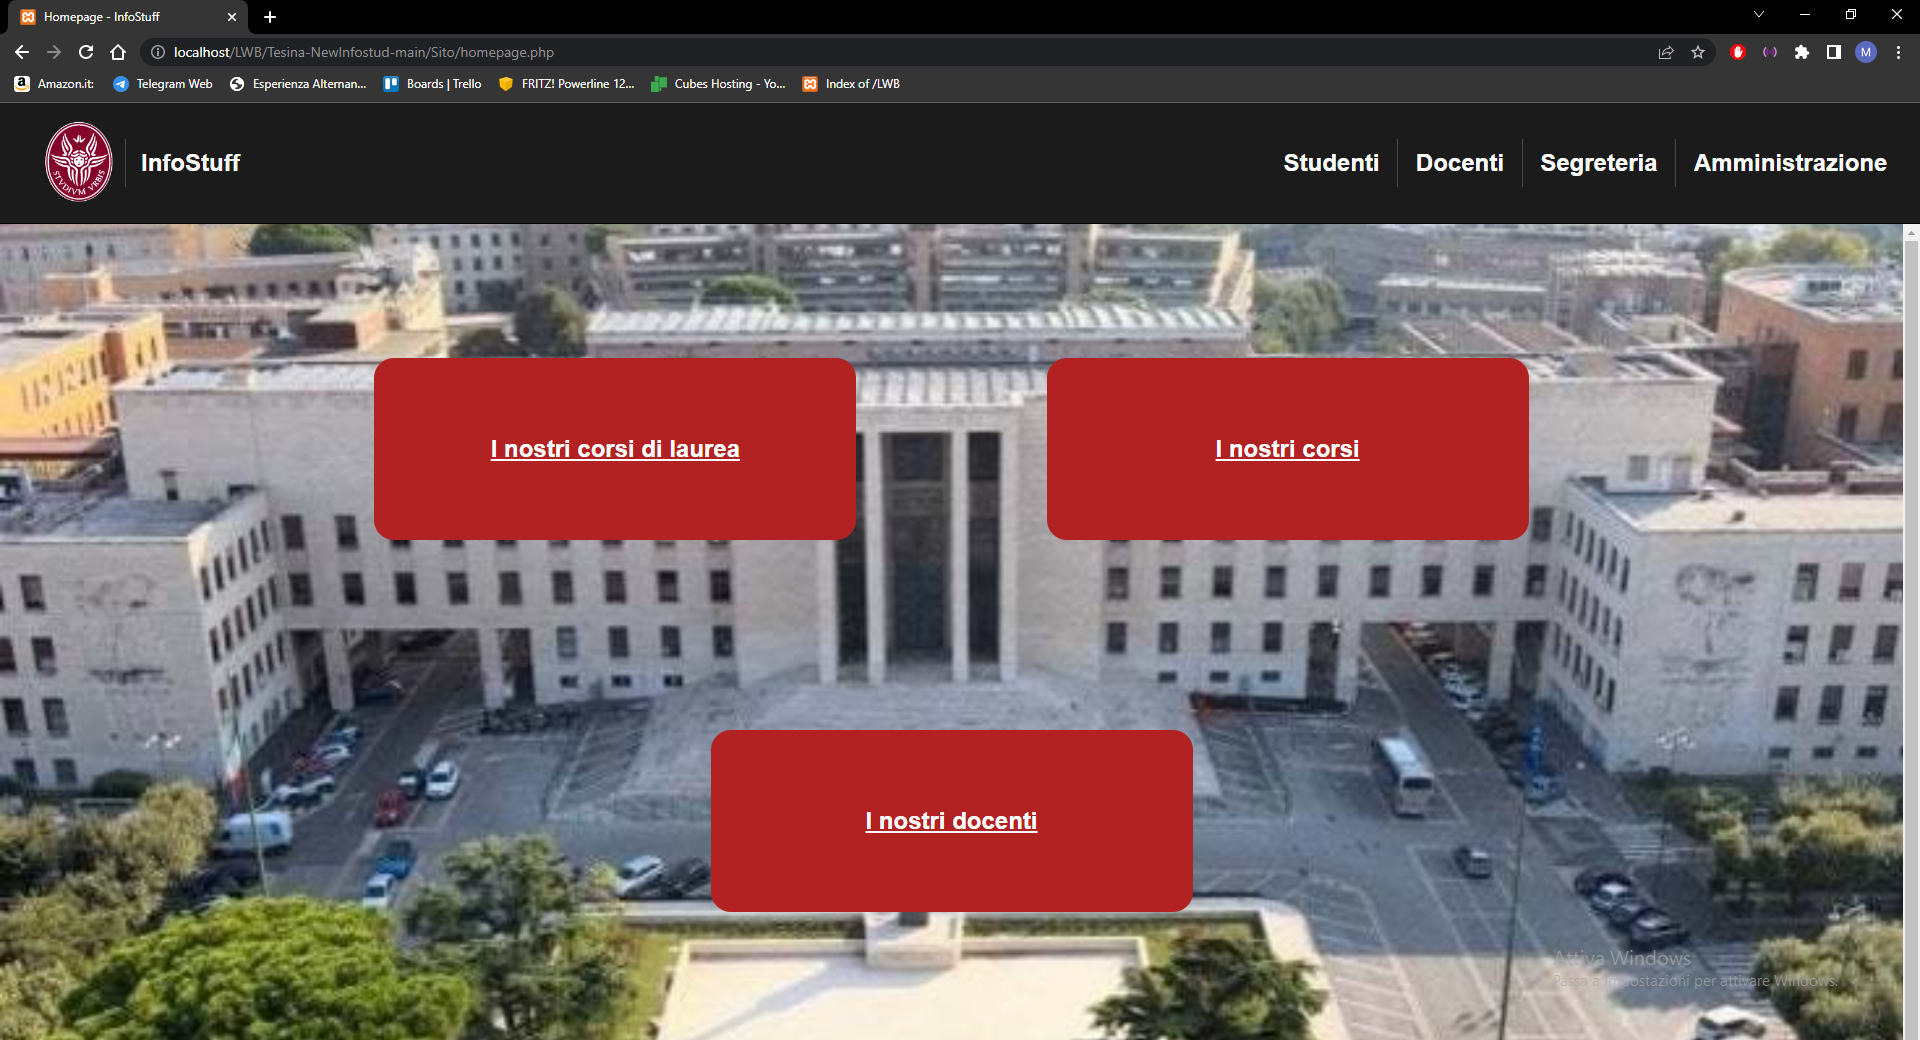
\includegraphics[scale=0.3]{figura2-1.png}
\caption{Homepage del sito.}
\end{figure}

Tale pagina web è costituita da un'immagine di sfondo che accompagna tre blocchi principali, indicanti tre delle cinque funzionalità a disposizione di un utente visitatore: la visualizzazione dei corsi di laurea, dei corsi e dei docenti attualmente presenti presso la piattaforma. Nella parte superiore della pagina web, invece, possiamo apprezzare diversi pulsanti relativi ad ogni altra utenza in grado di usufruire dei servizi offerti dalla piattaforma: questi pulsanti rappresentano dei collegamenti a varie pagine di login, presso le quali l'utente è in grado di autenticarsi. Qualora non disponesse di credenziali, invece, l'utente può registrarsi tramite l'opportuna funzionalità messa a disposizione all'interno delle form di login appena citate.

\medskip

\subsection{Visualizzare i corsi di laurea}

A partire dalla homepage del sito, riportata in figura 2.1, è possibile interagire con il blocco ''\emph{I nostri corsi di laurea}'': facendo click sulla scritta, infatti, l'utente verrà reindirizzato verso una pagina web simile a quella riportata in figura 2.2, nella quale viene presentato un elenco di tutti i corsi di laurea attualmente registrati presso la piattaforma. Le singole voci dell'elenco dispongono di un bottone che, se premuto, reindirizzerà l'utente verso una pagina web di visualizzazione di tutti i corsi relativi al corso di laurea precedentemente selezionato. Questa pagina web è mostrata in figura 2.3: anche qui, le singole voci dell'elenco presentato all'utente dispongono di un bottone che, se premuto, lo reindirizzerà verso un'ulteriore pagina web, mostrata in figura 2.4, avente uno scopo puramente informativo sui dettagli del singolo corso.

\begin{figure}
\centering
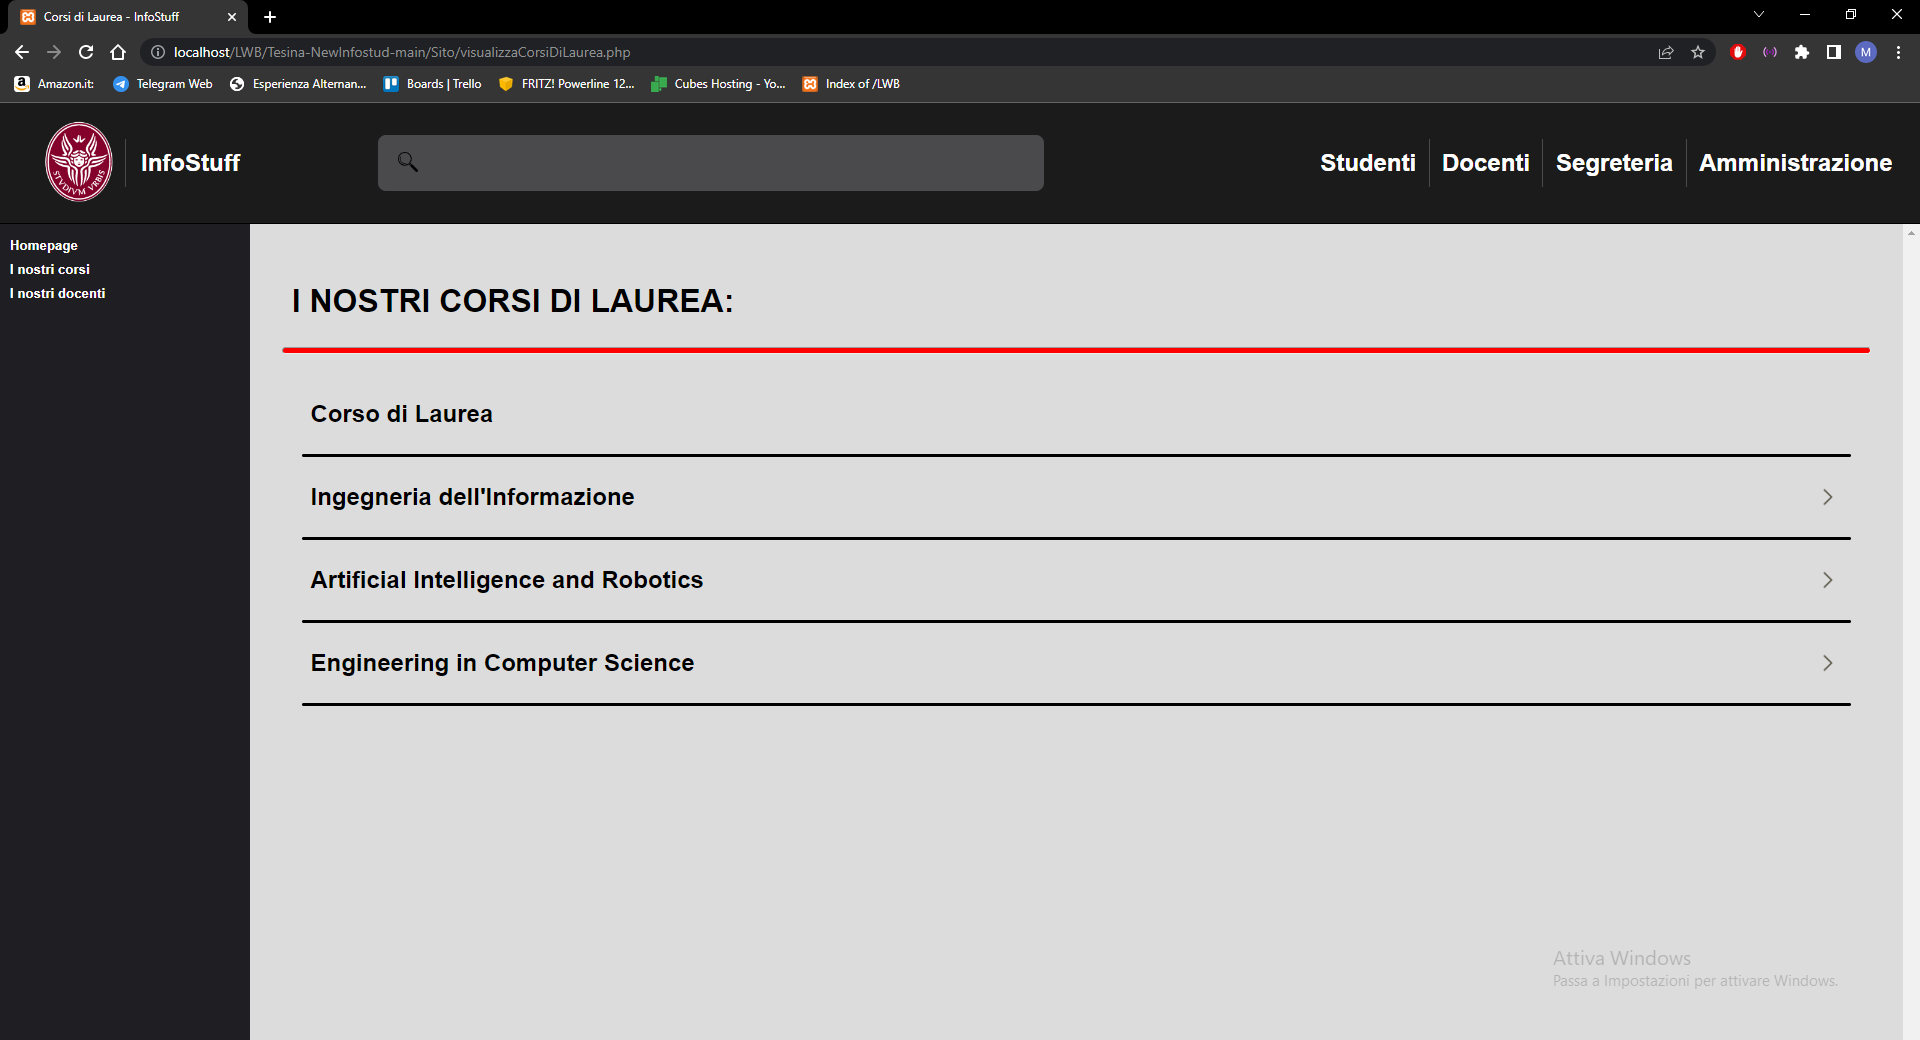
\includegraphics[scale=0.3]{figura2-2.png}
\caption{Visualizzazione dei corsi di laurea.}
\end{figure}

\begin{figure}
\centering
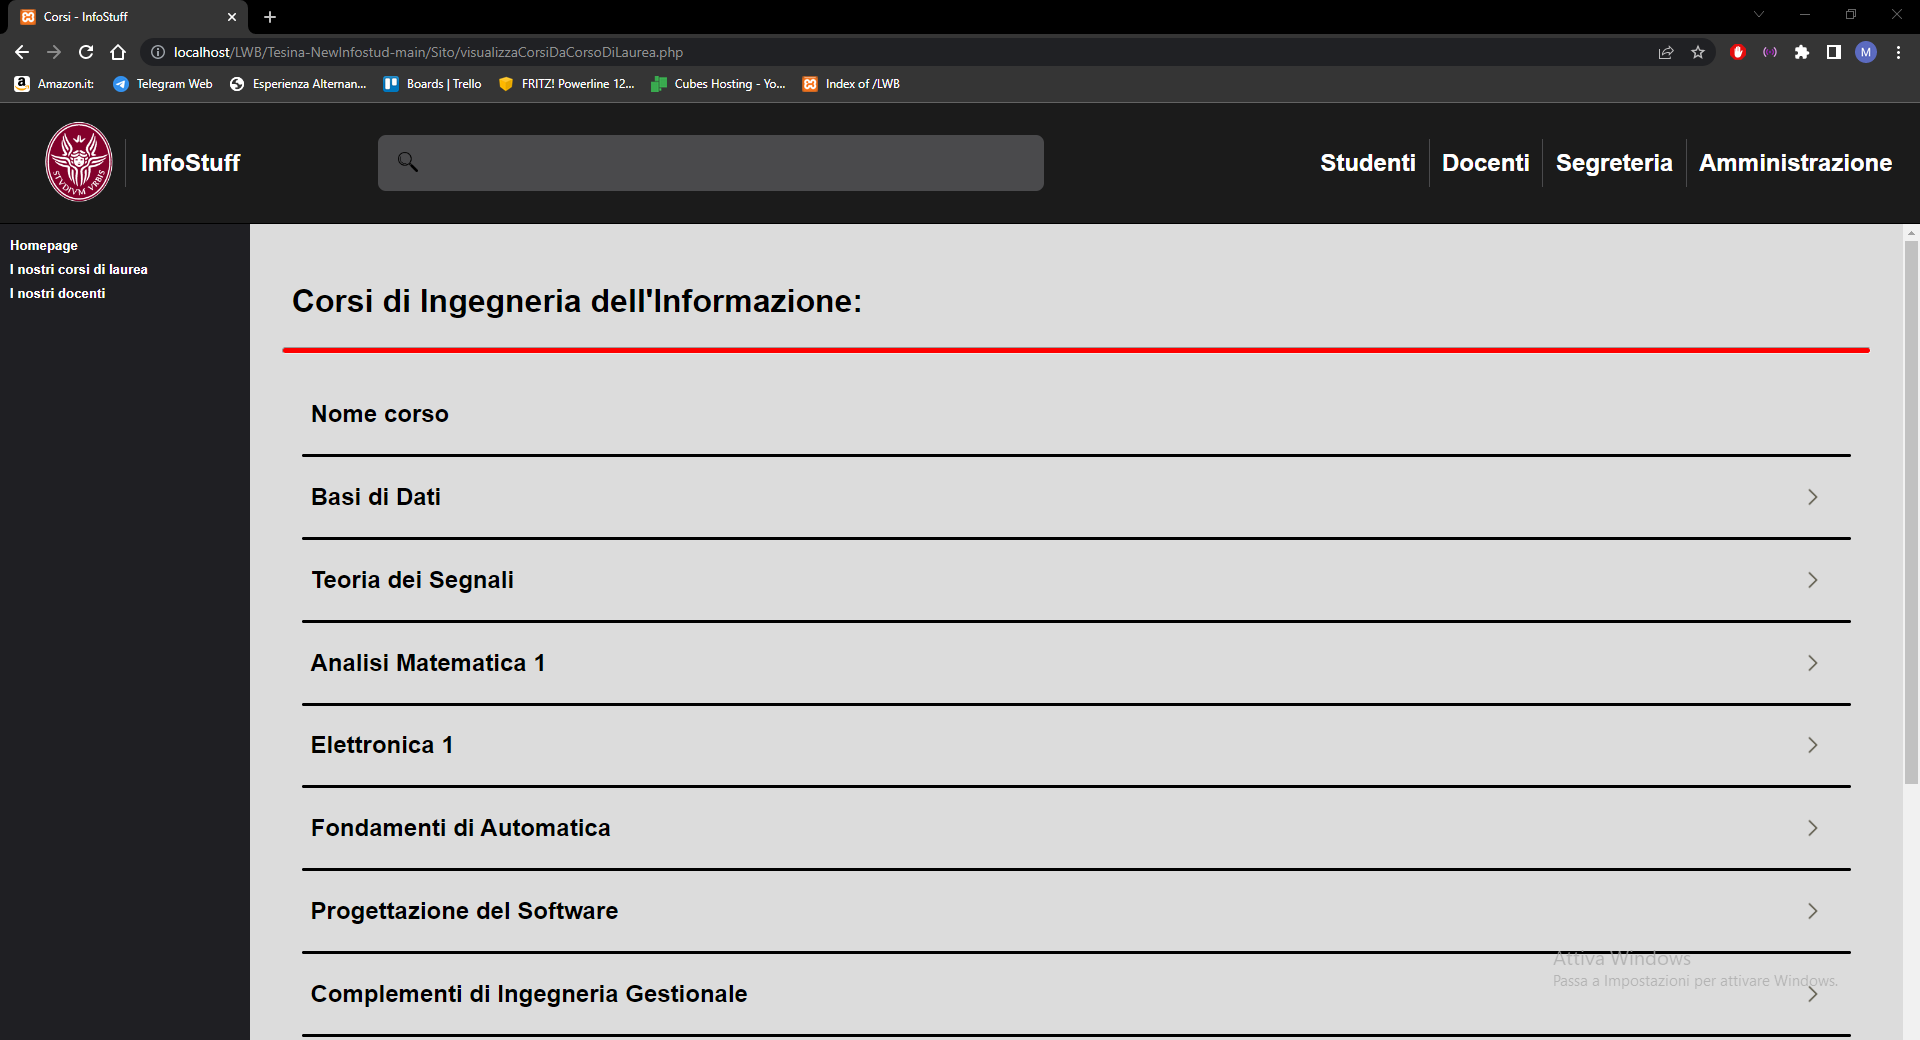
\includegraphics[scale=0.3]{figura2-3.png}
\caption{Visualizzazione dei corsi relativi ad un corso di laurea.}
\end{figure}

\begin{figure}
\centering
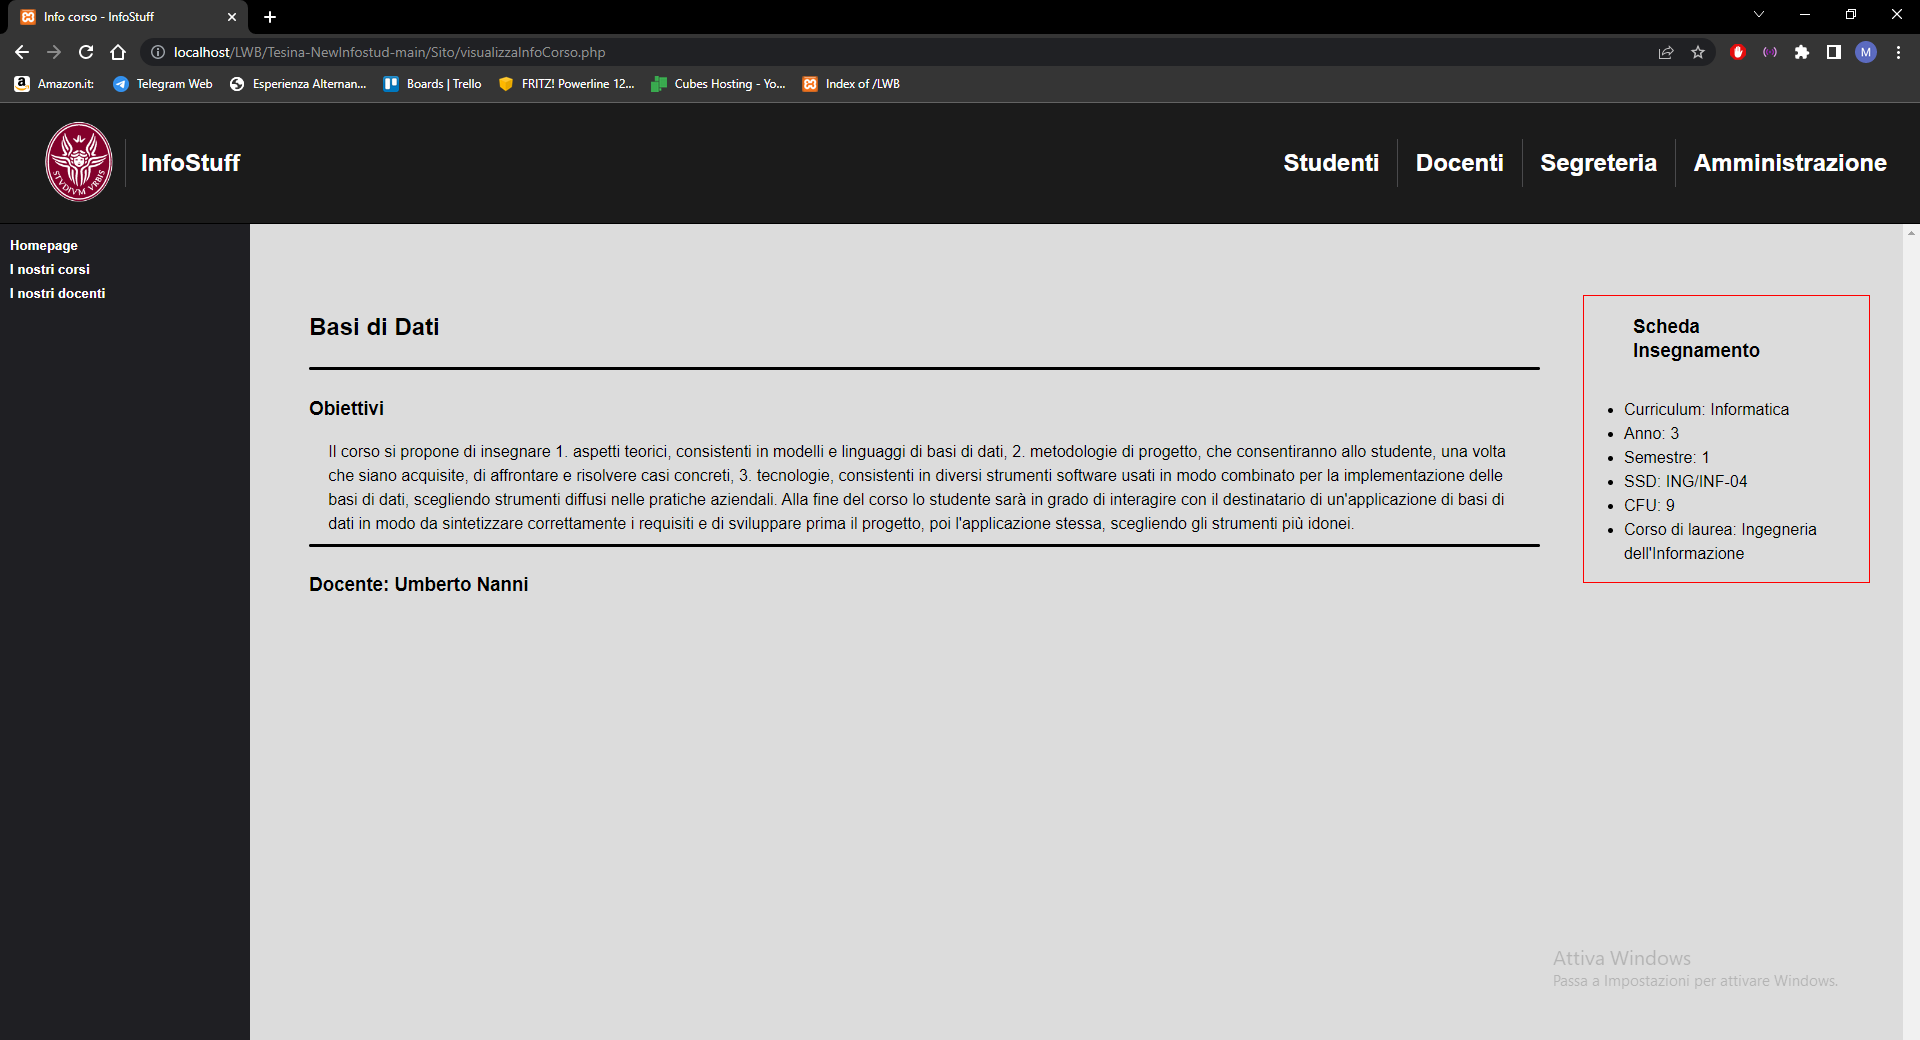
\includegraphics[scale=0.3]{figura2-4.png}
\caption{Visualizzazione delle informazioni relative ad un corso.}
\end{figure}

La visualizzazione delle singole voci dei vari elenchi di presentazione citati in questo paragrafo è facilitata dalla presenza di una barra di ricerca nella parte superiore delle varie pagine web. Per effettuare una ricerca filtrata, sarà sufficiente inserire il nome di un corso/corso di laurea (o anche solo parte di esso): premendo poi sull'opportuna icona costituita da una lente di ingrandimento, verranno presentati a schermo tutti i risultati della ricerca.

\medskip

\subsection{Visualizzare i corsi}

A partire dalla homepage del sito, riportata in figura 2.1, è possibile interagire con il blocco ''\emph{I nostri corsi}'': facendo click sulla scritta, infatti, l'utente verrà reindirizzato verso una pagina web simile a quella riportata in figura 2.5, nella quale viene presentato un elenco di tutti i corsi attualmente registrati presso la piattaforma, con l'ulteriore informazione relativa al rispettivo corso di laurea di afferenza. Le singole voci dell'elenco presentato all'utente dispongono di un bottone che, se premuto, lo reindirizzerà verso un'ulteriore pagina web, mostrata in figura 2.4, avente uno scopo puramente informativo sui dettagli del singolo corso.

\begin{figure}
\centering
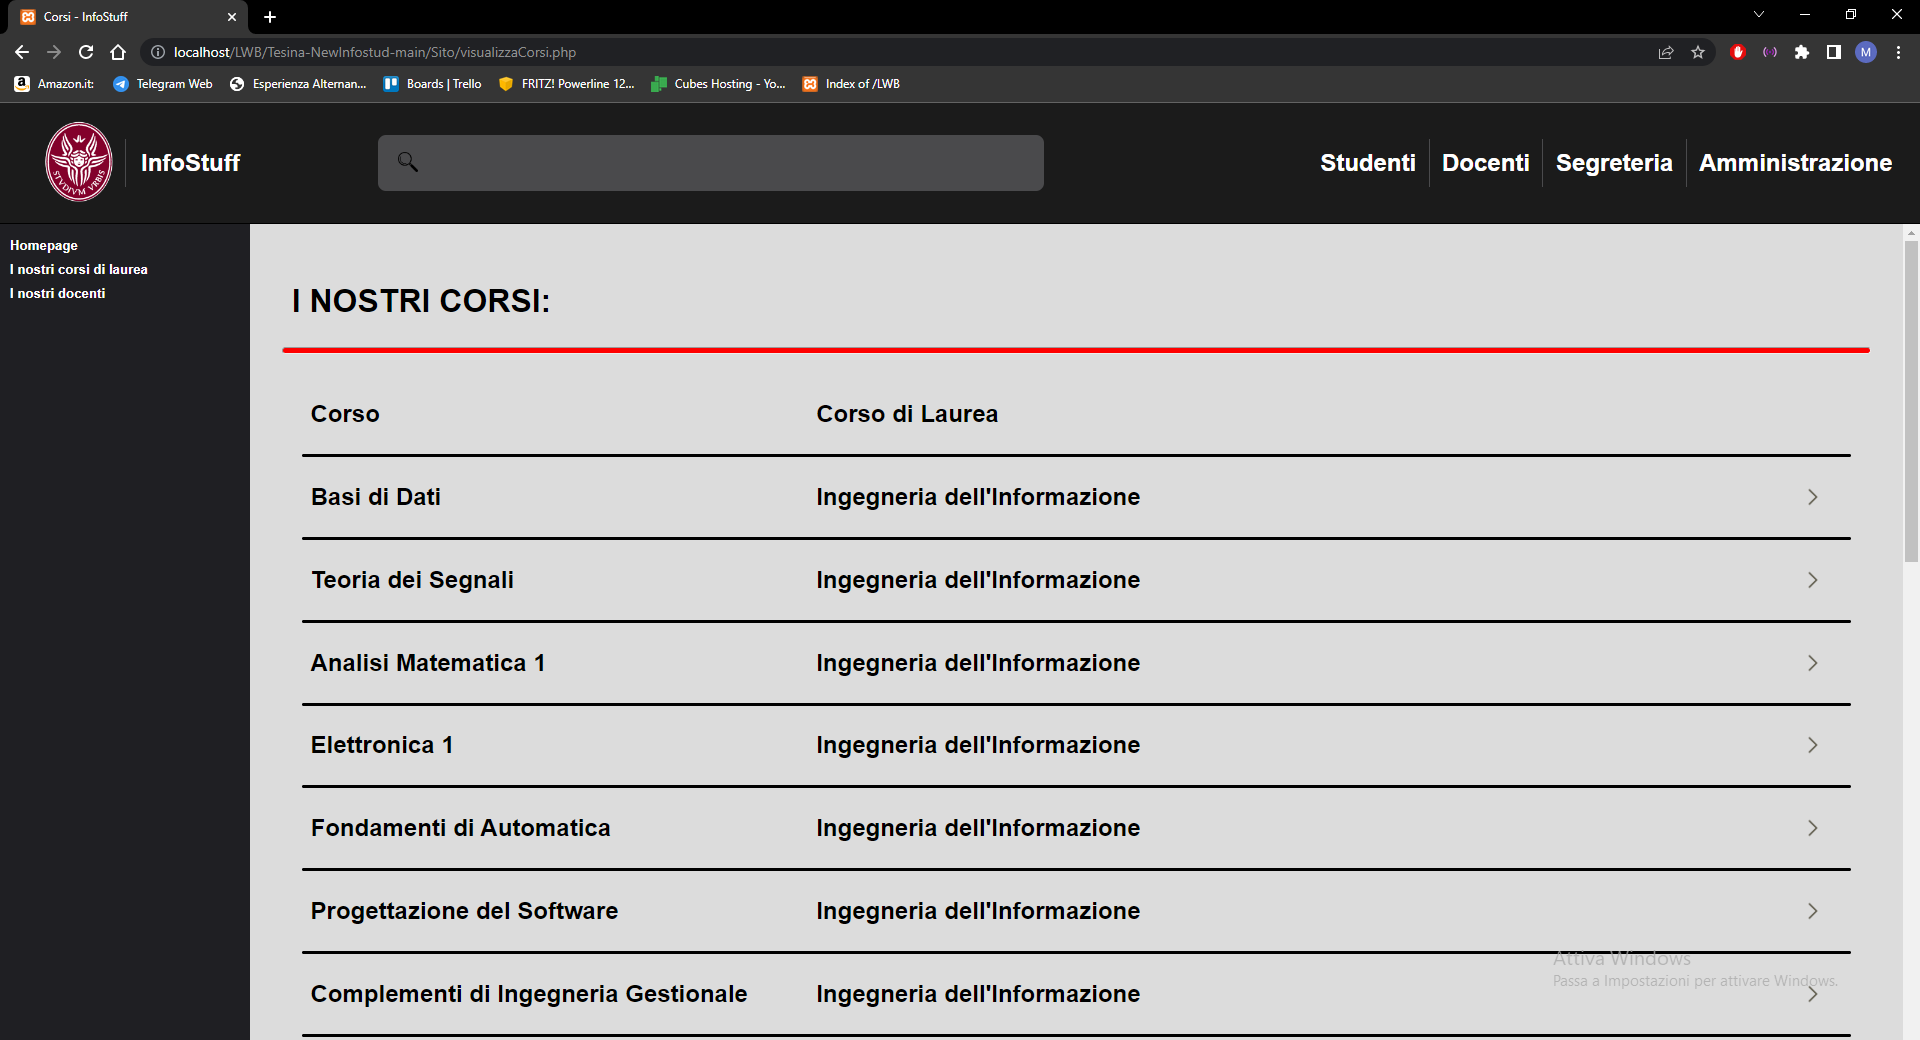
\includegraphics[scale=0.3]{figura2-5.png}
\caption{Visualizzazione dei corsi.}
\end{figure}

La visualizzazione delle singole voci dell'elenco dei corsi citato in questo paragrafo è facilitata dalla presenza di una barra di ricerca nella parte superiore della pagina web. Per effettuare una ricerca filtrata, sarà sufficiente inserire il nome di un corso (o anche solo parte di esso): premendo poi sull'opportuna icona costituita da una lente di ingrandimento, verranno presentati a schermo tutti i risultati della ricerca.

\medskip

\subsection{Visualizzare i docenti}

A partire dalla homepage del sito, riportata in figura 2.1, è possibile interagire con il blocco ''\emph{I nostri docenti}'': facendo click sulla scritta, infatti, l'utente verrà reindirizzato verso una pagina web simile a quella riportata in figura 2.6, nella quale viene presentato un elenco di tutti i docenti attualmente registrati presso la piattaforma, in ordine alfabetico. È inoltre presente un'informazione aggiuntiva sugli insegnamenti di ciascun docente; per ragioni pratiche, la visualizzazione è limitata ad al più tre insegnamenti per ciascun docente.

\begin{figure}
\centering
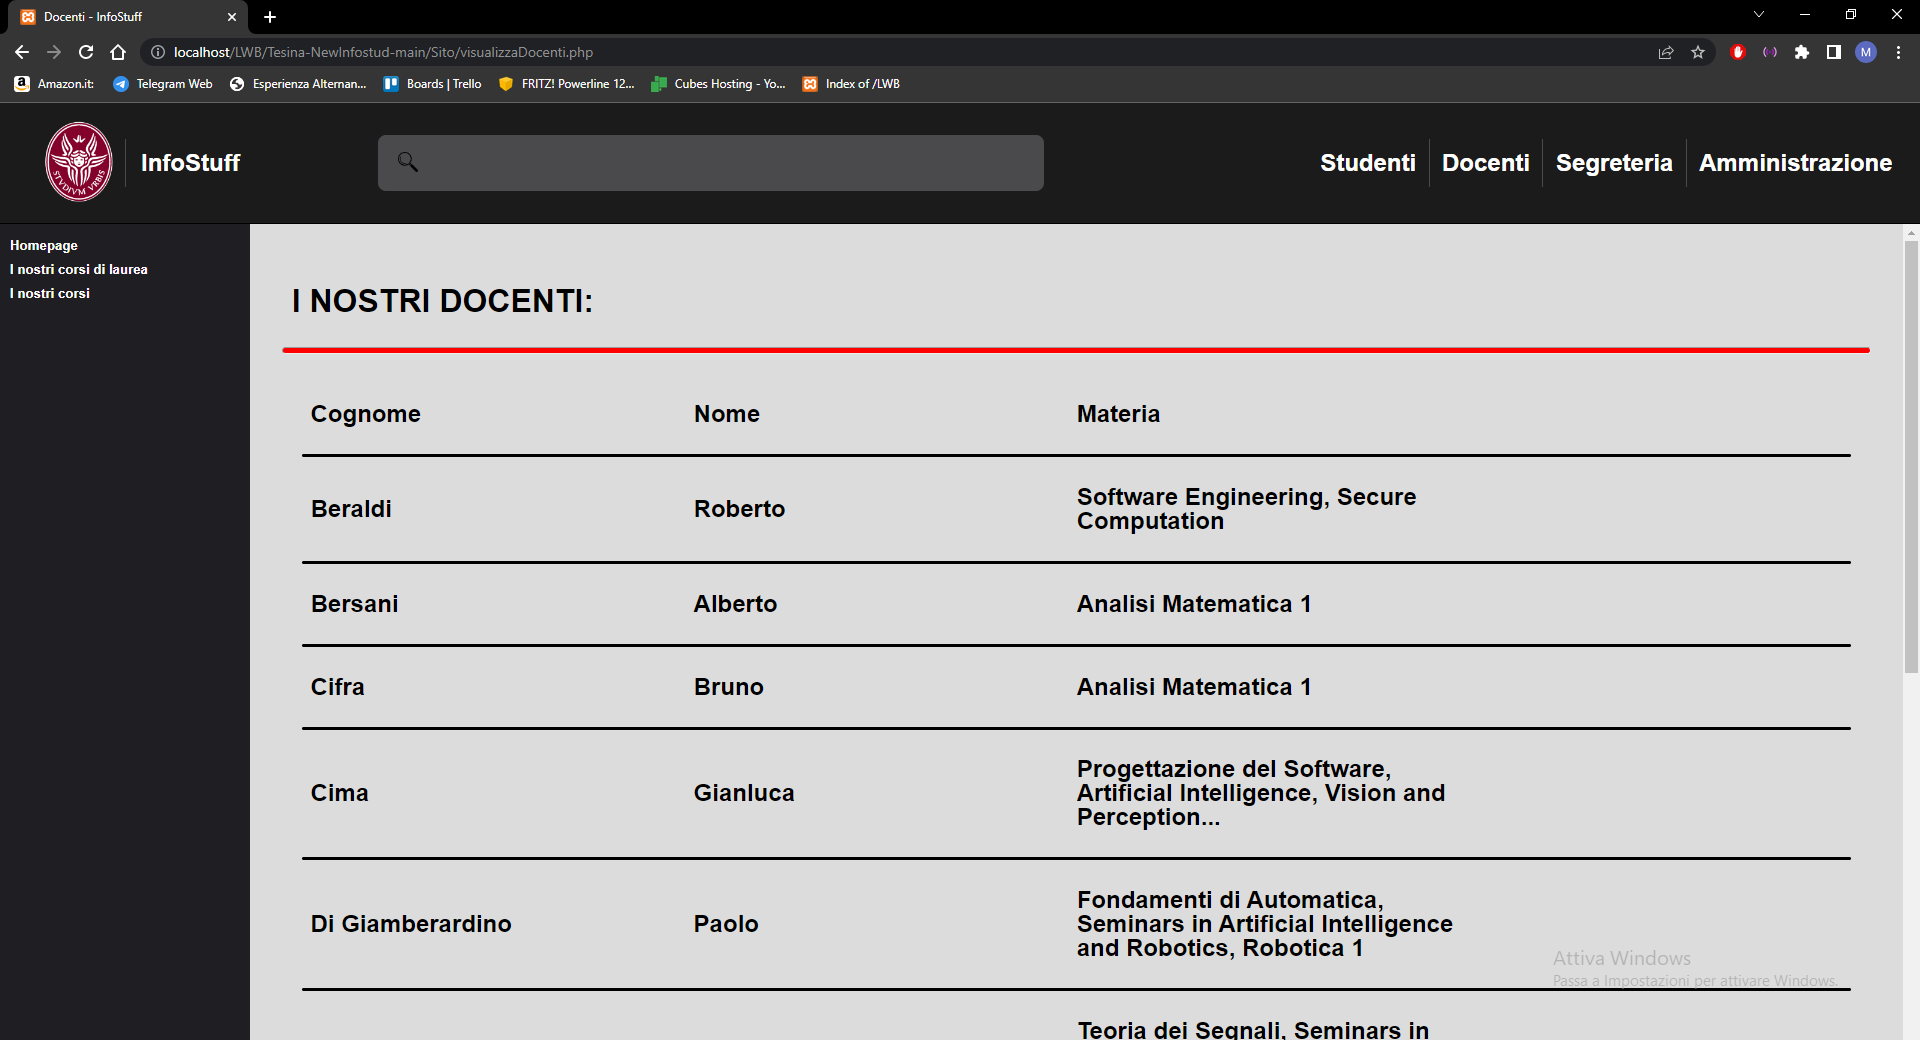
\includegraphics[scale=0.3]{figura2-6.png}
\caption{Visualizzazione dei docenti.}
\end{figure}

La visualizzazione delle singole voci dell'elenco dei docenti citato in questo paragrafo è facilitata dalla presenza di una barra di ricerca nella parte superiore della pagina web. Per effettuare una ricerca filtrata, sarà sufficiente inserire il cognome/nome di un docente (o anche solo parte di esso): premendo poi sull'opportuna icona costituita da una lente di ingrandimento, verranno presentati a schermo tutti i risultati della ricerca.

\medskip

\subsection{Autenticarsi}

A partire da una qualsiasi pagina web fra quelle citate in precedenza, è possibile interagire con i pulsanti \emph{Studenti}, \emph{Docenti}, \emph{Segreteria} e \emph{Amministrazione}, che hanno lo scopo di reindirizzare l'utente verso le rispettive pagine di login; una pagina web di login di esempio è mostrata in figura 2.7. Per le utenze che intendano autenticarsi come studente o come docente, sarà necessario disporre di una matricola e di una password; per le utenze che intendano autenticarsi come segretario o come amministratore, invece, sarà necessario disporre di uno username e di una password.

\begin{figure}
\centering
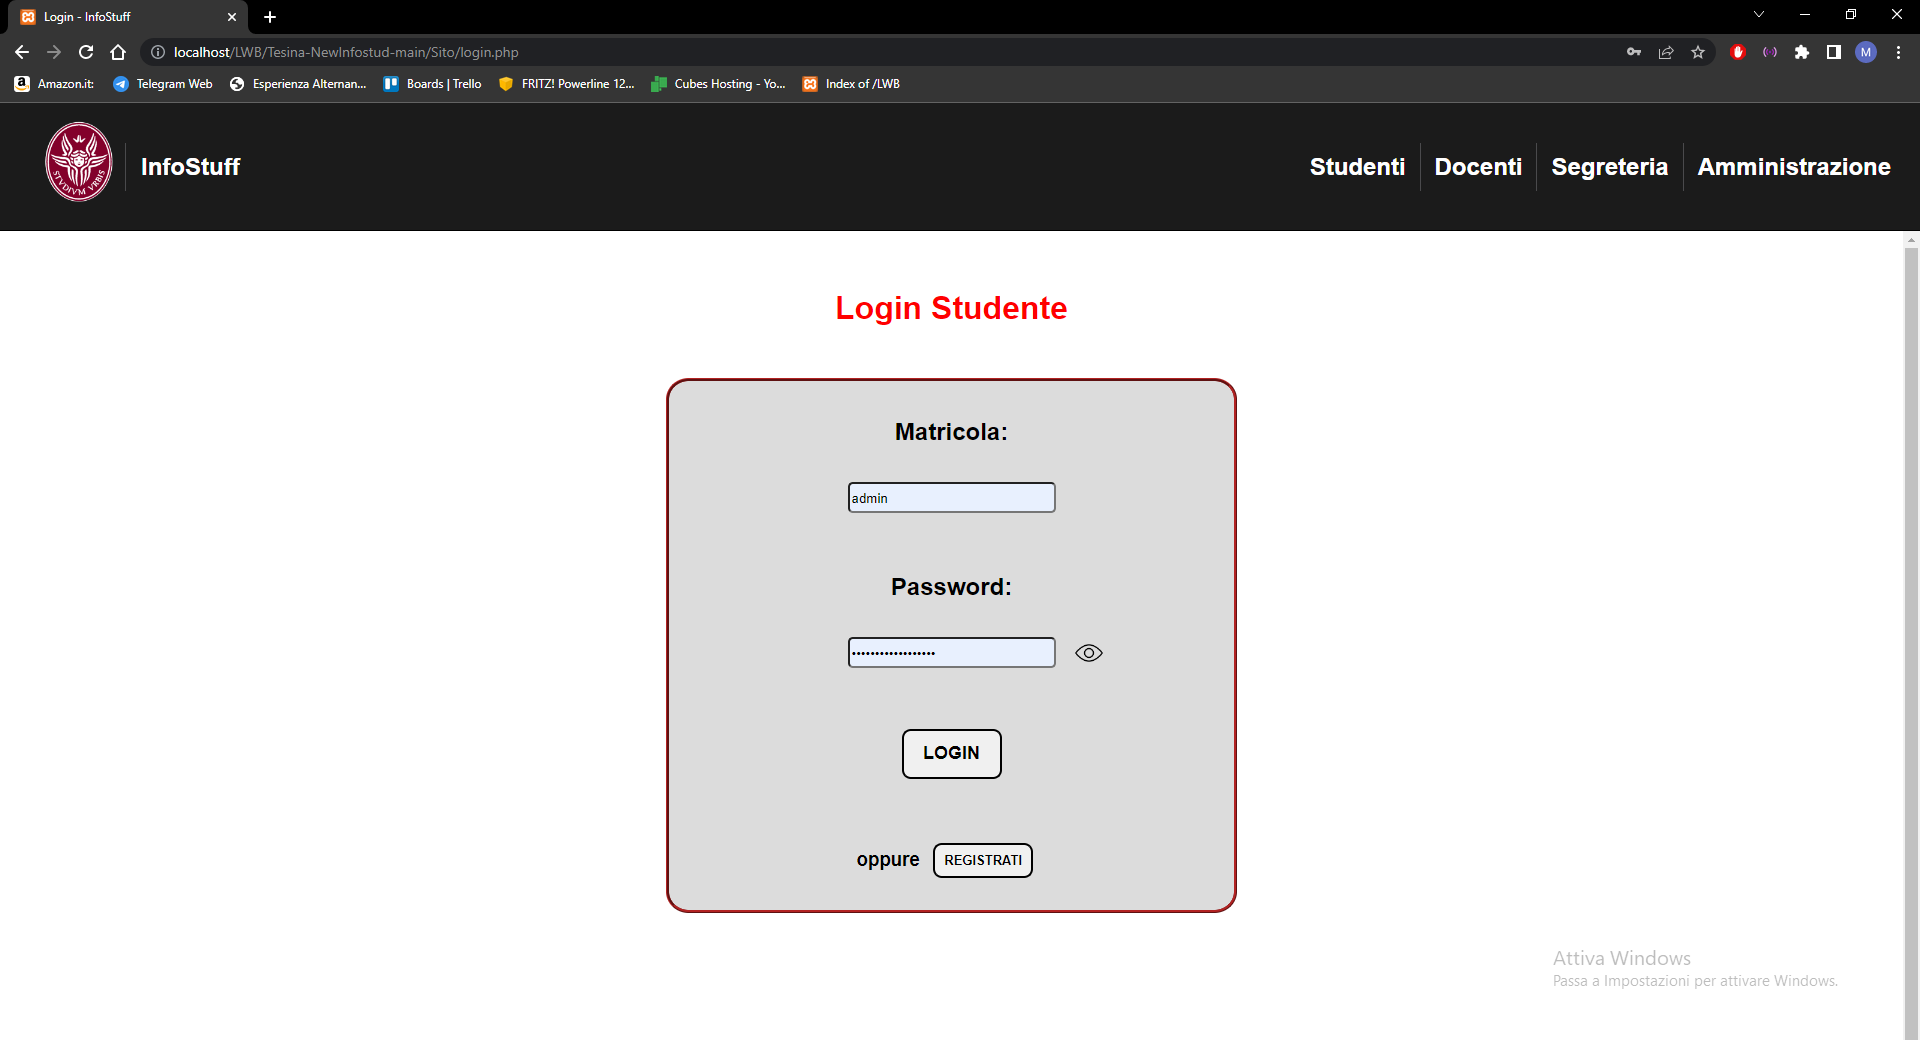
\includegraphics[scale=0.3]{figura2-7.png}
\caption{Form di login di esempio.}
\end{figure}

Una volta autenticato, l'utente cesserà di essere un semplice visitatore della piattaforma, potendo usufruire di molteplici ulteriori funzionalità, dipendentemente dalla tipologia di utenza con la quale l'utente stesso ha scelto di autenticarsi per la corrente sessione.

\medskip

\subsection{Registrarsi}

Qualora l'utente visitatore non disponesse di alcune credenziali, non potendo di fatto autenticarsi nella piattaforma, potrebbe decidere di registrarsi presso di essa: sarà sufficiente premere l'apposito pulsante \emph{registrati} mostrato nella parte inferiore della figura 2.7. In base al tipo di utenza selezionata, l'utente, in seguito alla pressione del pulsante appena citato, verrà reindirizzato verso una form di registrazione alla piattaforma; generalmente, sarà richiesto all'utente di specificare alcuni dati personali, così come la scelta di una password. Nel caso particolare di uno studente, verrà richiesto anche lo specifico corso di laurea al quale l'utente desidera iscriversi; una pagina web di registrazione di esempio è mostrata in figura 2.8.

\begin{figure}
\centering
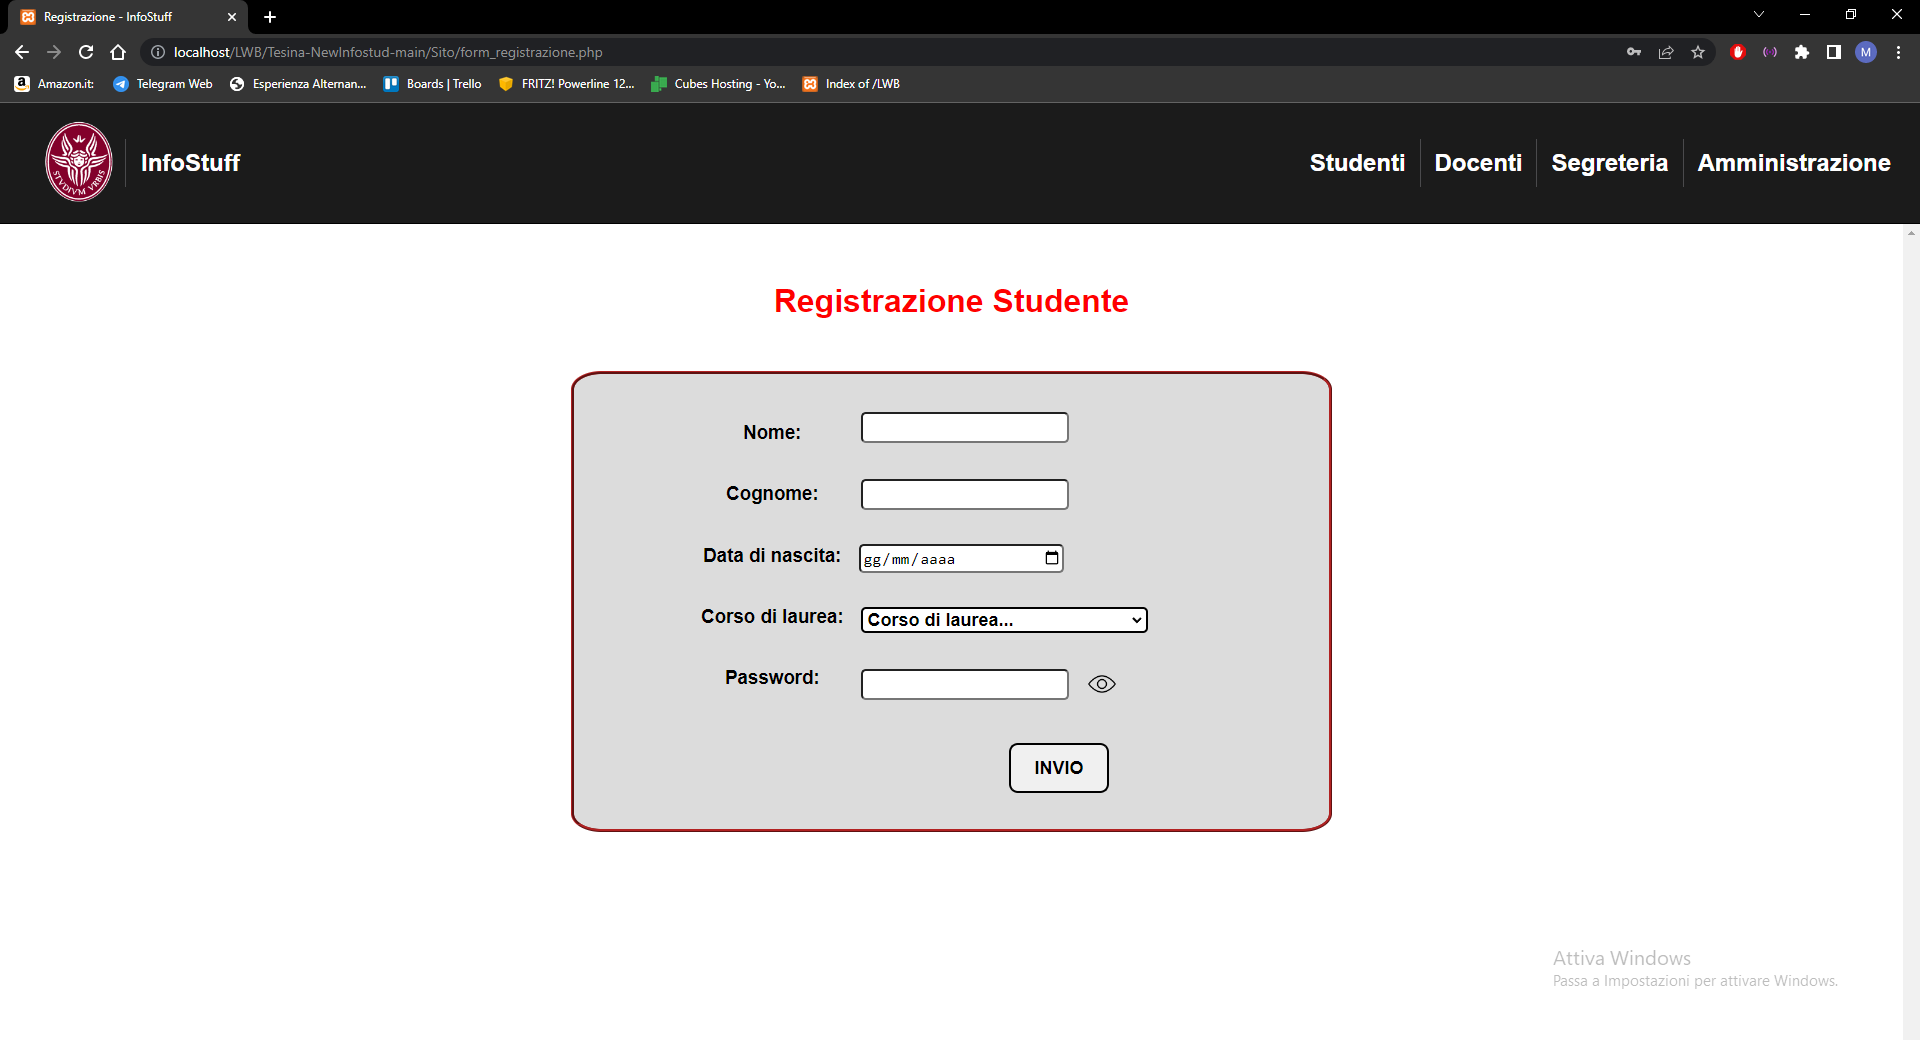
\includegraphics[scale=0.3]{figura2-8.png}
\caption{Form di registrazione di esempio.}
\end{figure}

\medskip
\medskip

\section{Studente}

In questa sezione analizziamo e descriviamo tutte le funzionalità accessibili ad un'utenza di tipo \emph{studente}. Assumeremo quindi che l'utilizzatore della piattaforma abbia eseguito l'accesso tramite l'apposita funzionalità di login sopra descritta. Prima di approfondire le varie funzionalità, analizziamo la schermata che si presenterà all'utente dopo aver fatto accesso alla piattaforma; più in particolare, il menù laterale che si presenterà all'utente, mostrato in figura 2.9.

\begin{figure}
\centering
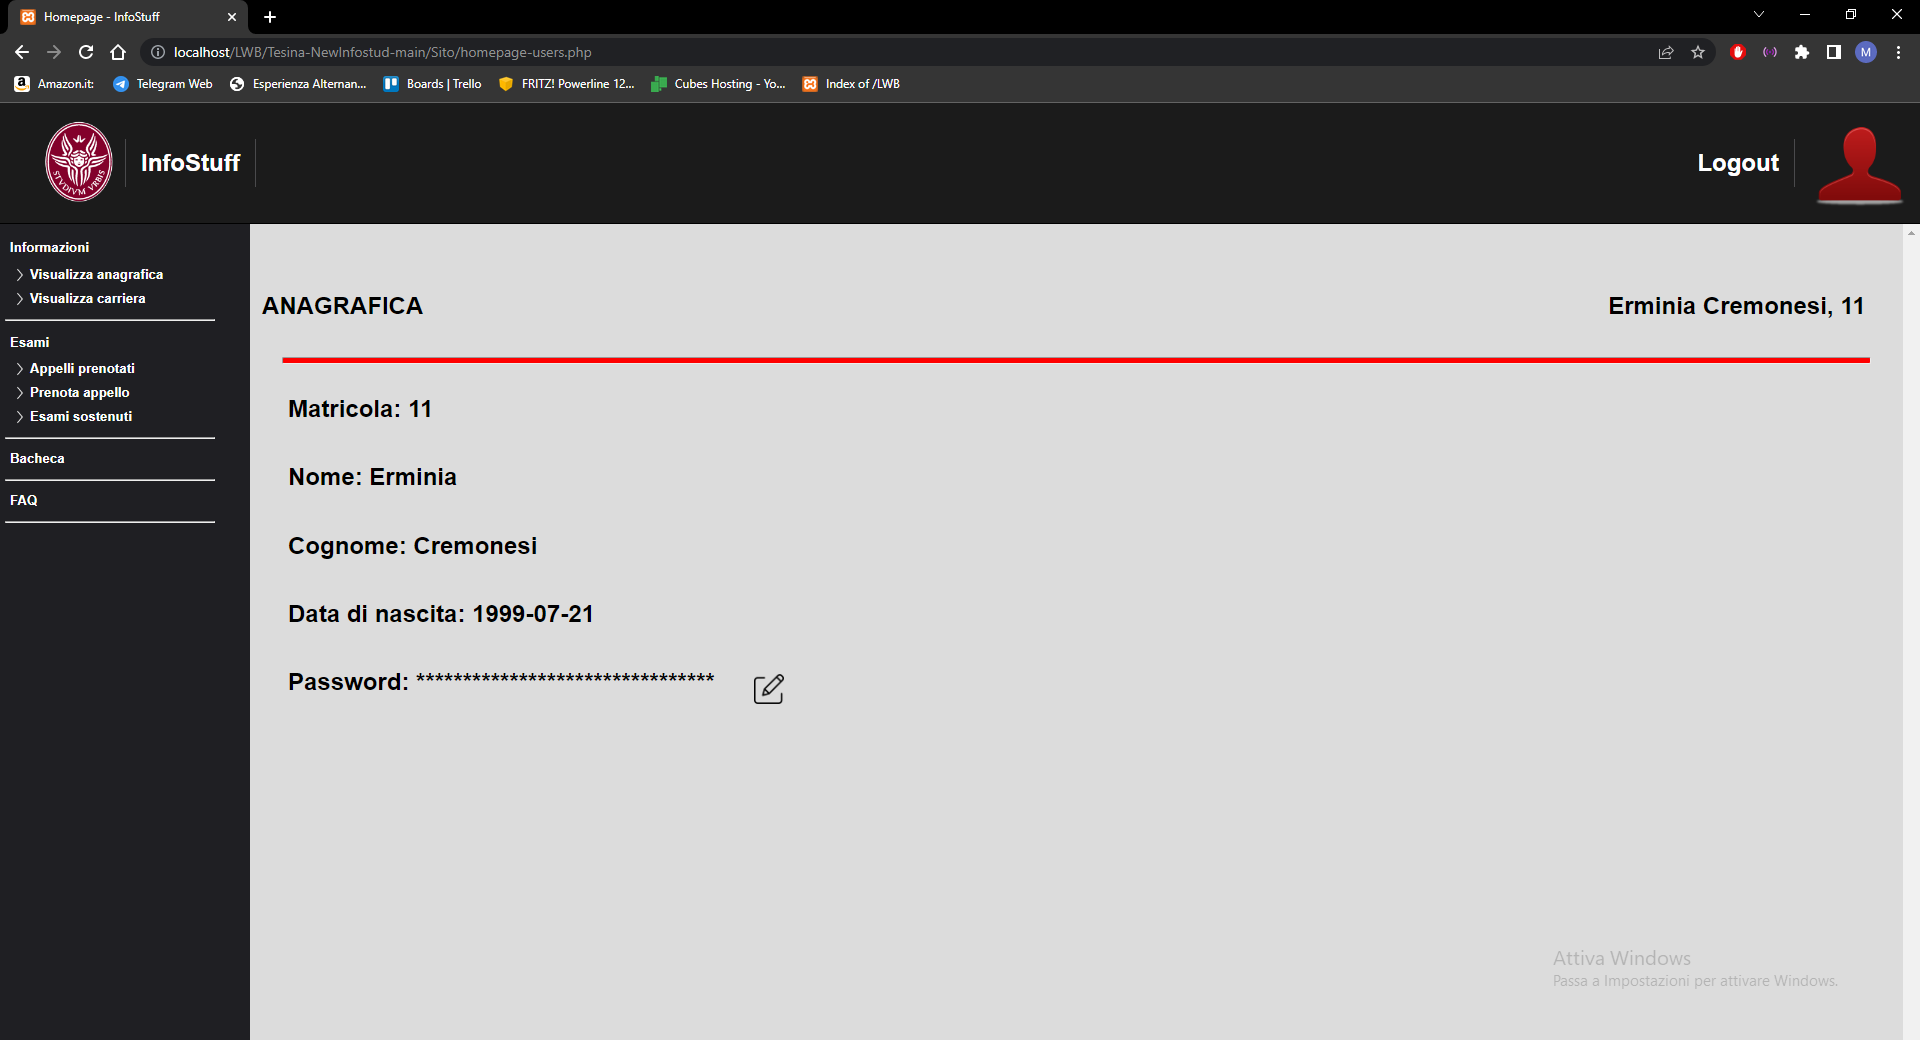
\includegraphics[scale=0.3]{figura2-9.png}
\caption{Homepage dell'utenza \emph{Studente}.}
\end{figure}

Tramite il suddetto menù, è possibile accedere a tutte le funzionalità riservate a questo tipo di utenza. Analizzeremo queste ultime nelle sezioni che seguono.

\medskip

\subsection{Visualizzare l'anagrafica}

Usufruibile dalla pagina home che si presenta all'utente un volta effettuato il login, la funzionalità di visualizzazione dell'anagrafica consiste nella stampa a video di tutte le informazioni personali associate all'utenza. Tra di esse, come mostrato in figura 2.9, troviamo nome, cognome, matricola, data di nascita e password; quest'ultima verrà visualizzata coperta da degli asterischi, che rappresentano la lunghezza della relativa password criptata secondo l'algoritmo di cifratura MD5. Come per ogni altra utenza nella piattaforma, uno studente può modificare la propria password (figura 2.10), premendo sull'apposita icona situata a fianco della password stessa.

\begin{figure}
\centering
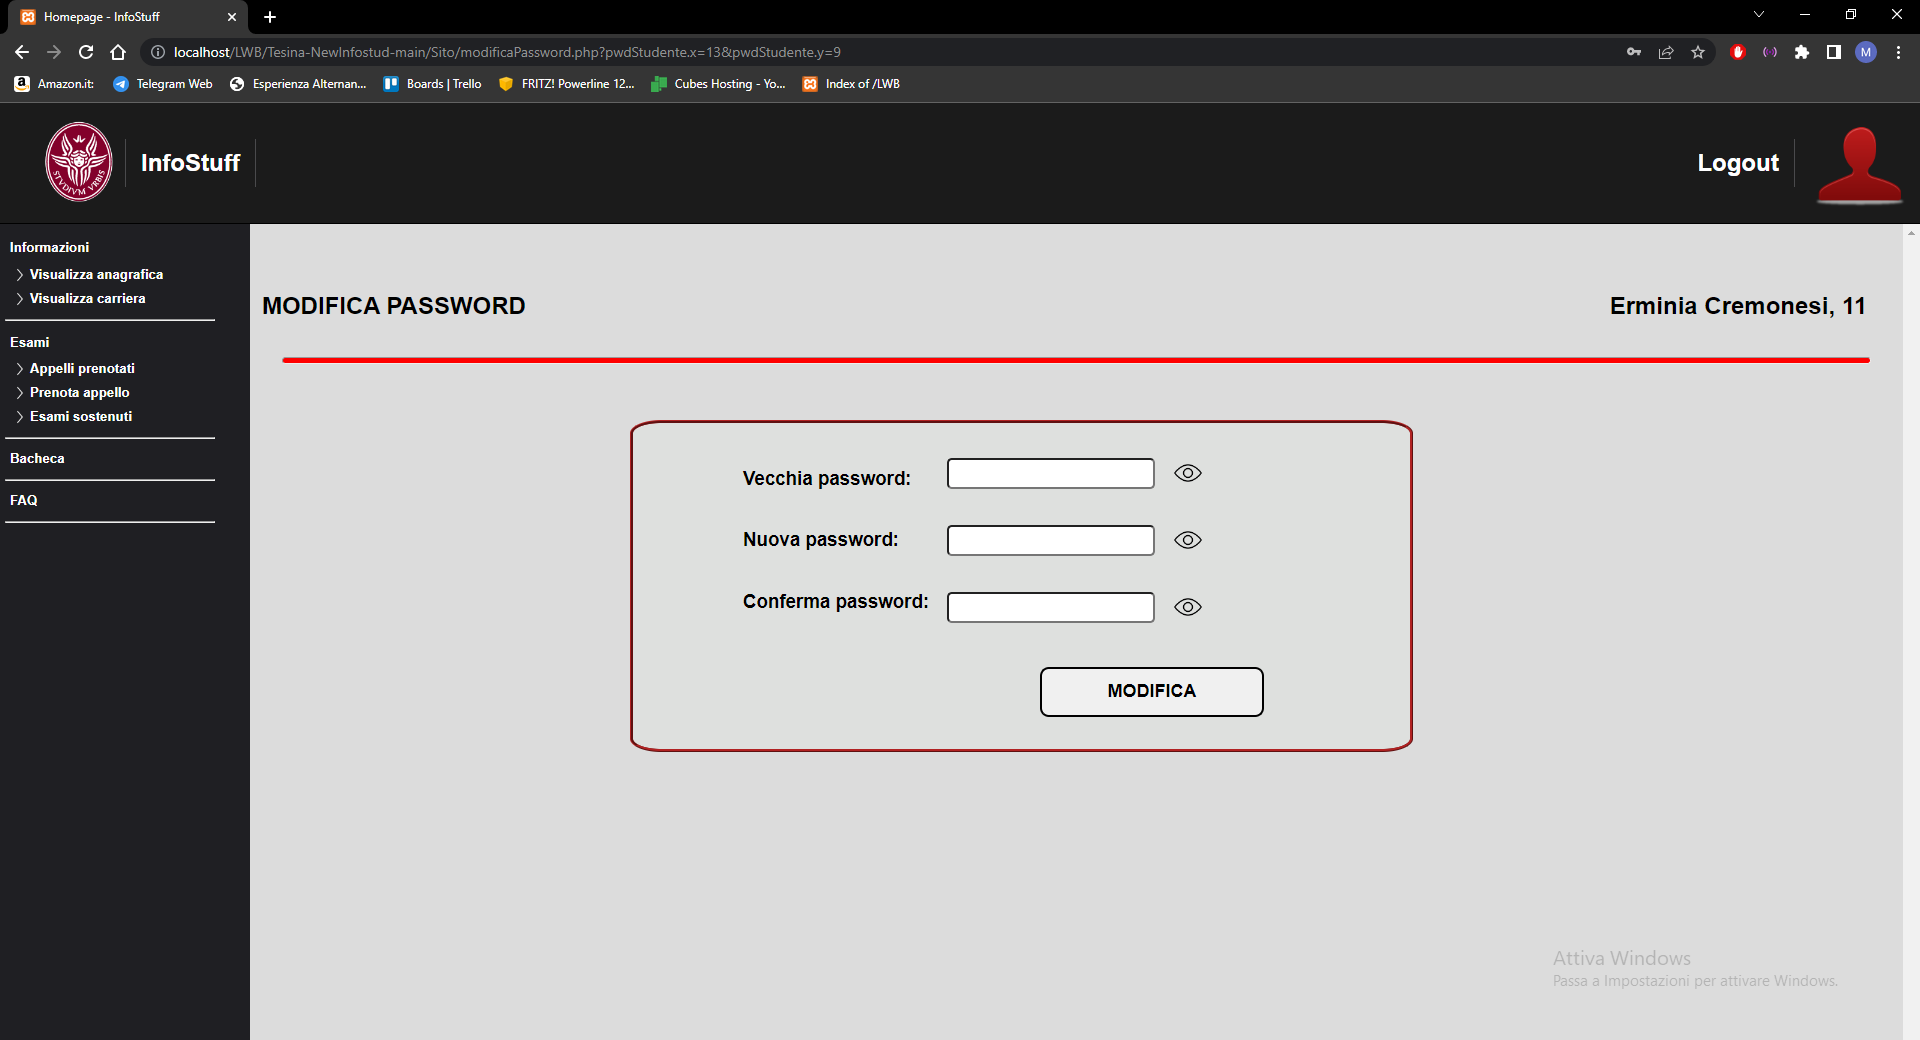
\includegraphics[scale=0.3]{figura2-10.png}
\caption{Form di modifica password.}
\end{figure}

\medskip

\subsection{Visualizzare la carriera}

A partire da una qualsiasi pagina web relativa all'utenza, è possibile cliccare sulla voce \emph{Visualizza carriera}, sotto la sezione \emph{Informazioni}, all'interno della barra laterale sita a sinistra della pagina stessa. L'utente verrà così reindirizzato ad una pagina web come quella in figura 2.11, nella quale verranno presentati a schermo i dati relativi a tutte le informazioni legate alla carriera dello studente autenticato nella sessione corrente. Come mostrato in figura, tali informazioni comprendono il corso di laurea cui si è iscritti, la propria reputazione totale, i CFU totali accumulati fino a quel momento e la propria media dei voti, risultato di tutti gli esami svolti fino a quel momento con esito positivo.

\begin{figure}
\centering
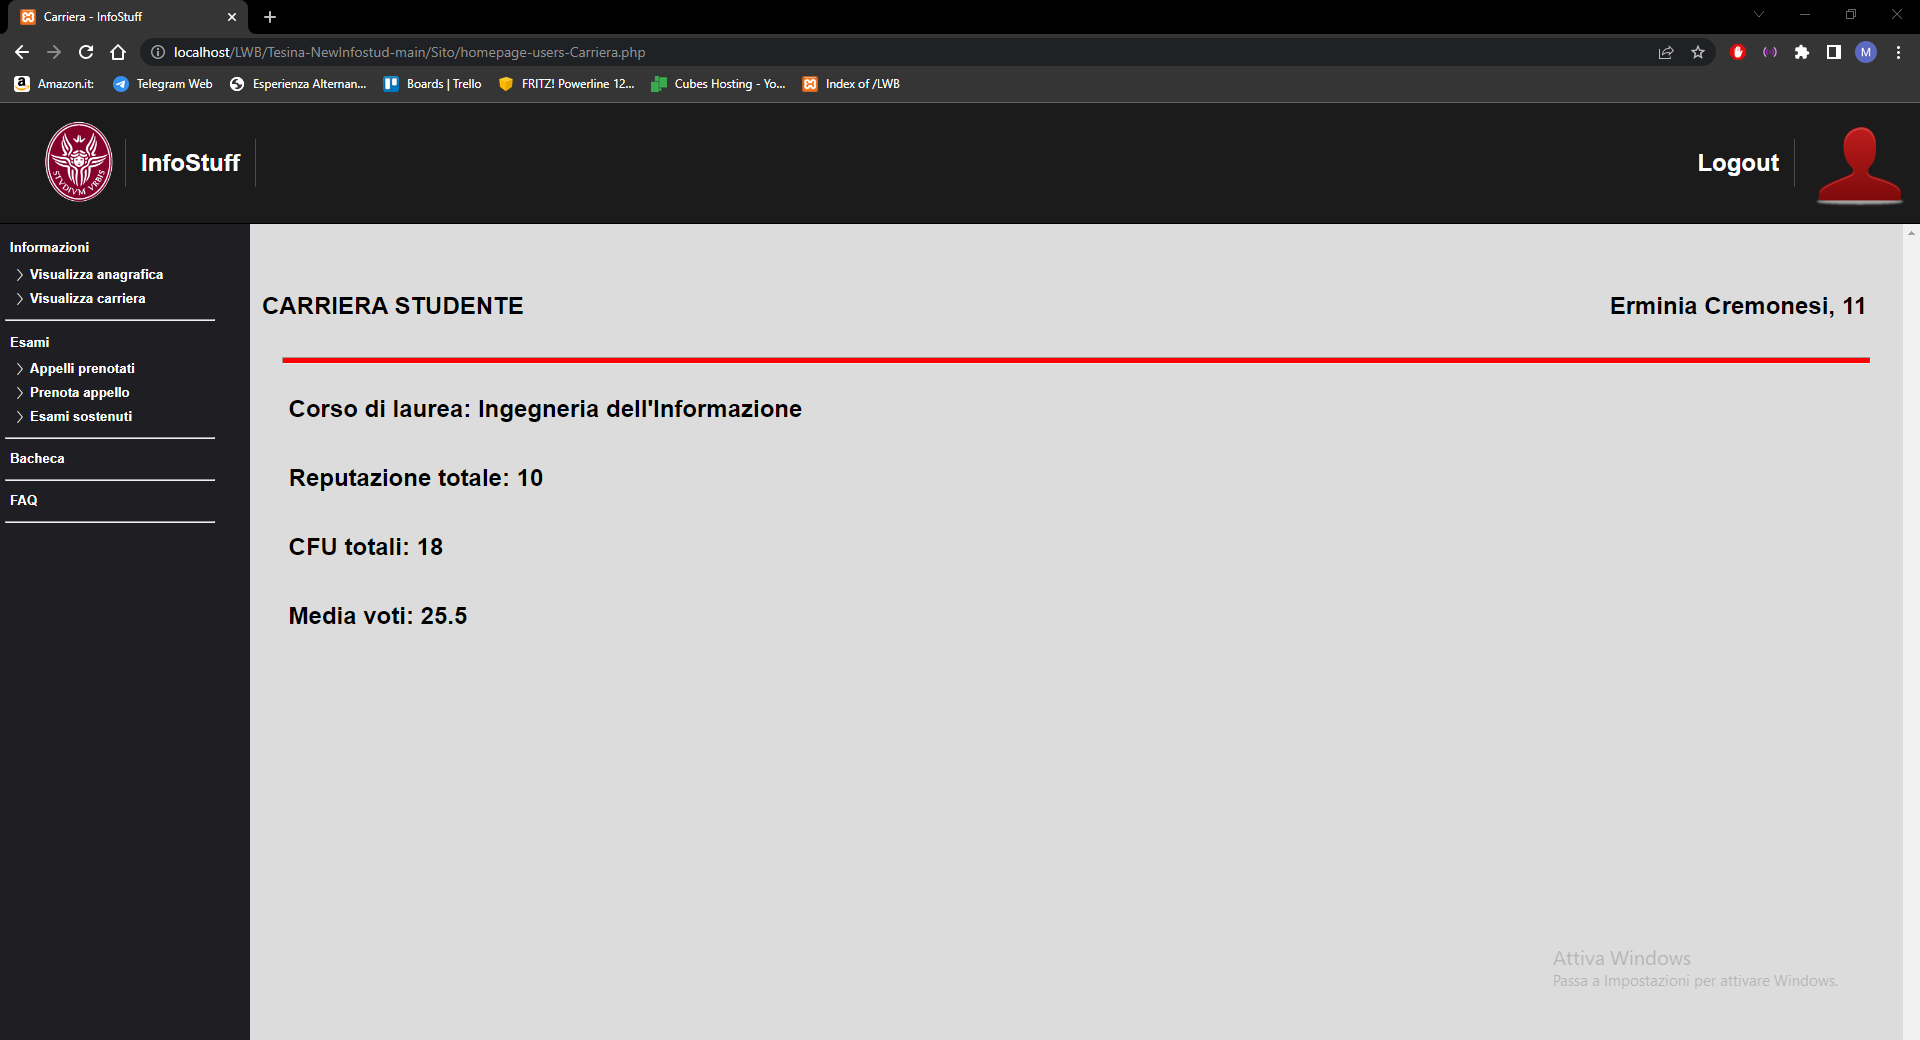
\includegraphics[scale=0.3]{figura2-11.png}
\caption{Pagina di visualizzazione delle informazioni relative alla carriera dello studente.}
\end{figure}

\medskip

\subsection{Visualizzare gli appelli prenotati}

A partire da una qualsiasi pagina web relativa all'utenza, è possibile cliccare sulla voce \emph{Appelli prenotati}, sotto la sezione \emph{Esami}, all'interno della barra laterale sita a sinistra della pagina stessa. L'utente verrà così reindirizzato ad una pagina web come quella in figura 2.12, nella quale verranno presentate a schermo tutte le prenotazioni relative agli appelli di esame prenotati dallo studente autenticato nella sessione corrente. In ogni momento, uno studente ha facoltà di annullare una prenotazione interagendo con l'apposito pulsante \emph{annulla}.

\begin{figure}
\centering
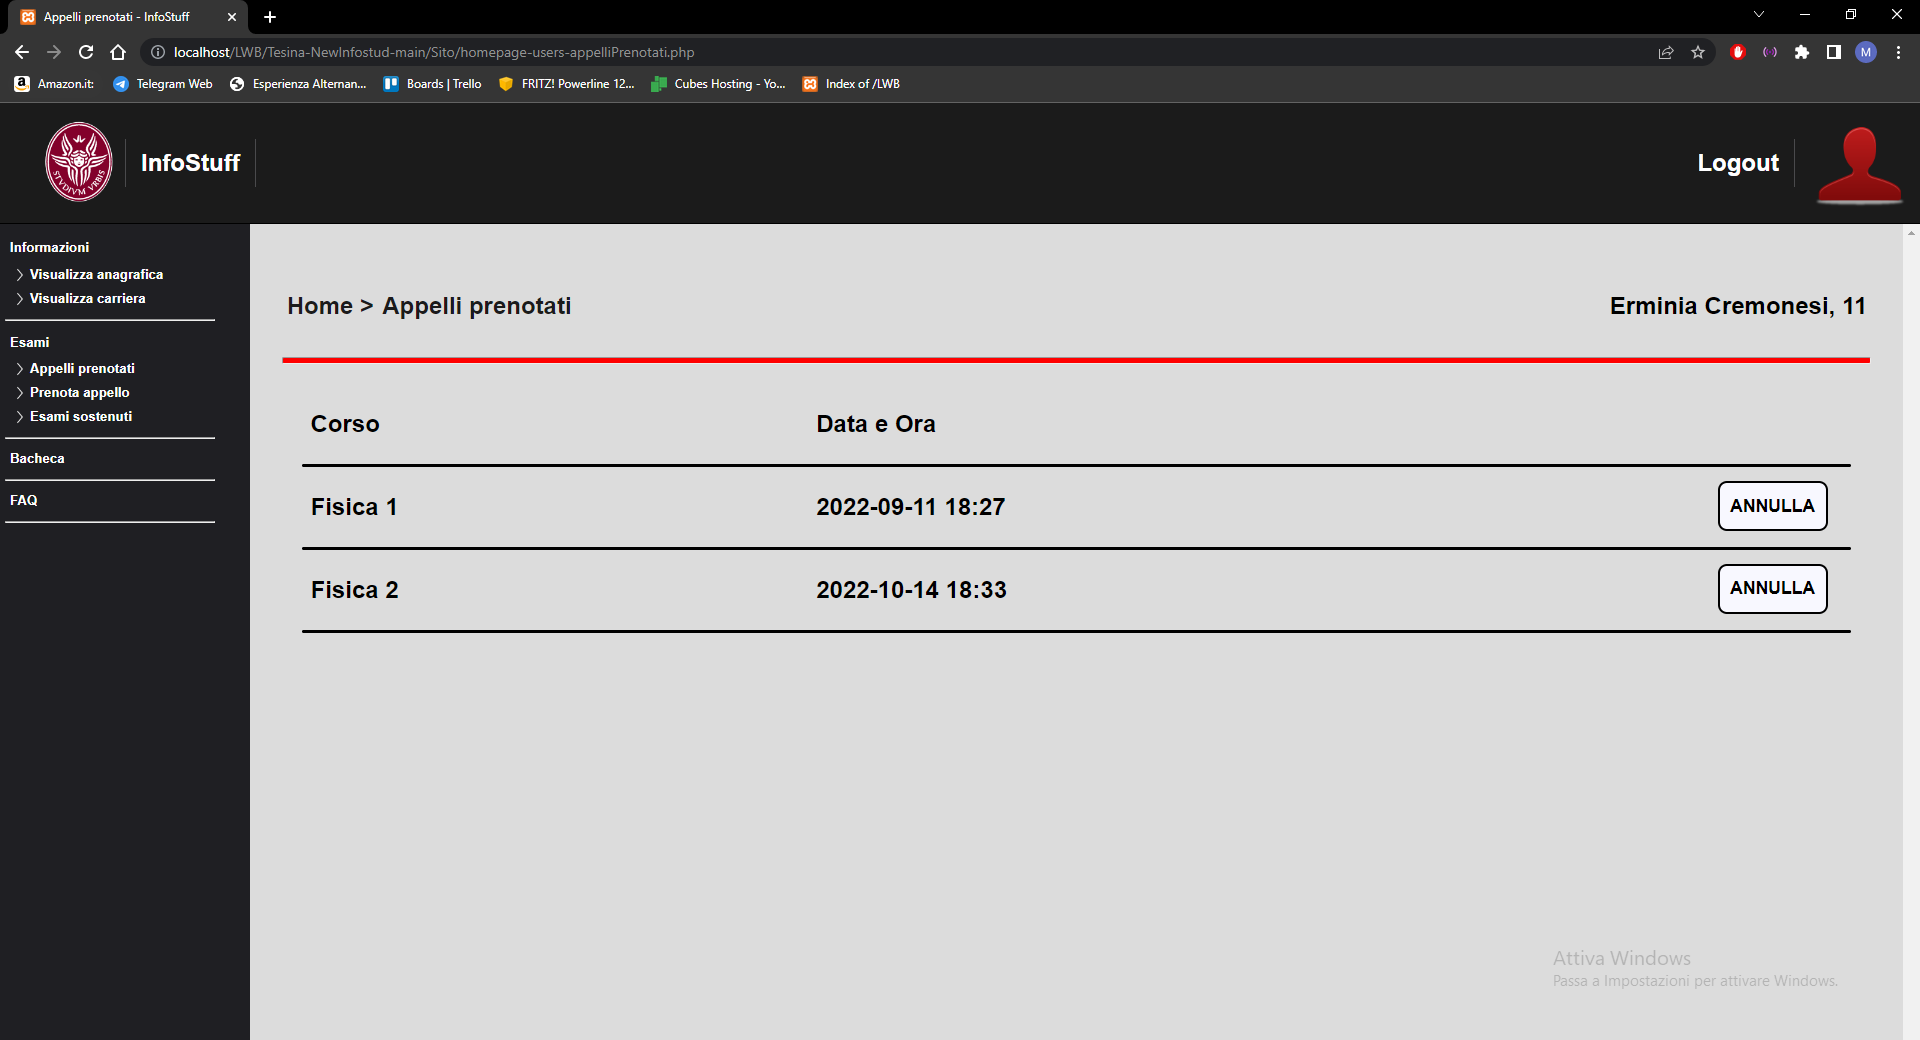
\includegraphics[scale=0.3]{figura2-12.png}
\caption{Pagina di visualizzazione dell'elenco degli appelli prenotati.}
\end{figure}

\medskip

\subsection{Visualizzare gli esami sostenuti}

A partire da una qualsiasi pagina web relativa all'utenza, è possibile cliccare sulla voce \emph{Esami sostenuti}, sotto la sezione \emph{Esami}, all'interno della barra laterale sita a sinistra della pagina stessa. L'utente verrà così reindirizzato ad una pagina web come quella in figura 2.13, nella quale verranno presentati a schermo tutti gli esami sostenuti dallo studente autenticato nella sessione corrente. In particolare, per ogni esame sostenuto, possiamo apprezzare sia la data di svolgimento dell'esame, che l'esito dello stesso.

Per quanto riguarda quest'ultima informazione - l'esito dell'esame - viene utilizzata una convenzione letterale per visualizzare eventuali fallimenti: la lettera \emph{B} identifica una bocciatura; la lettera \emph{R}, invece, identifica un ritiro.

\begin{figure}
\centering
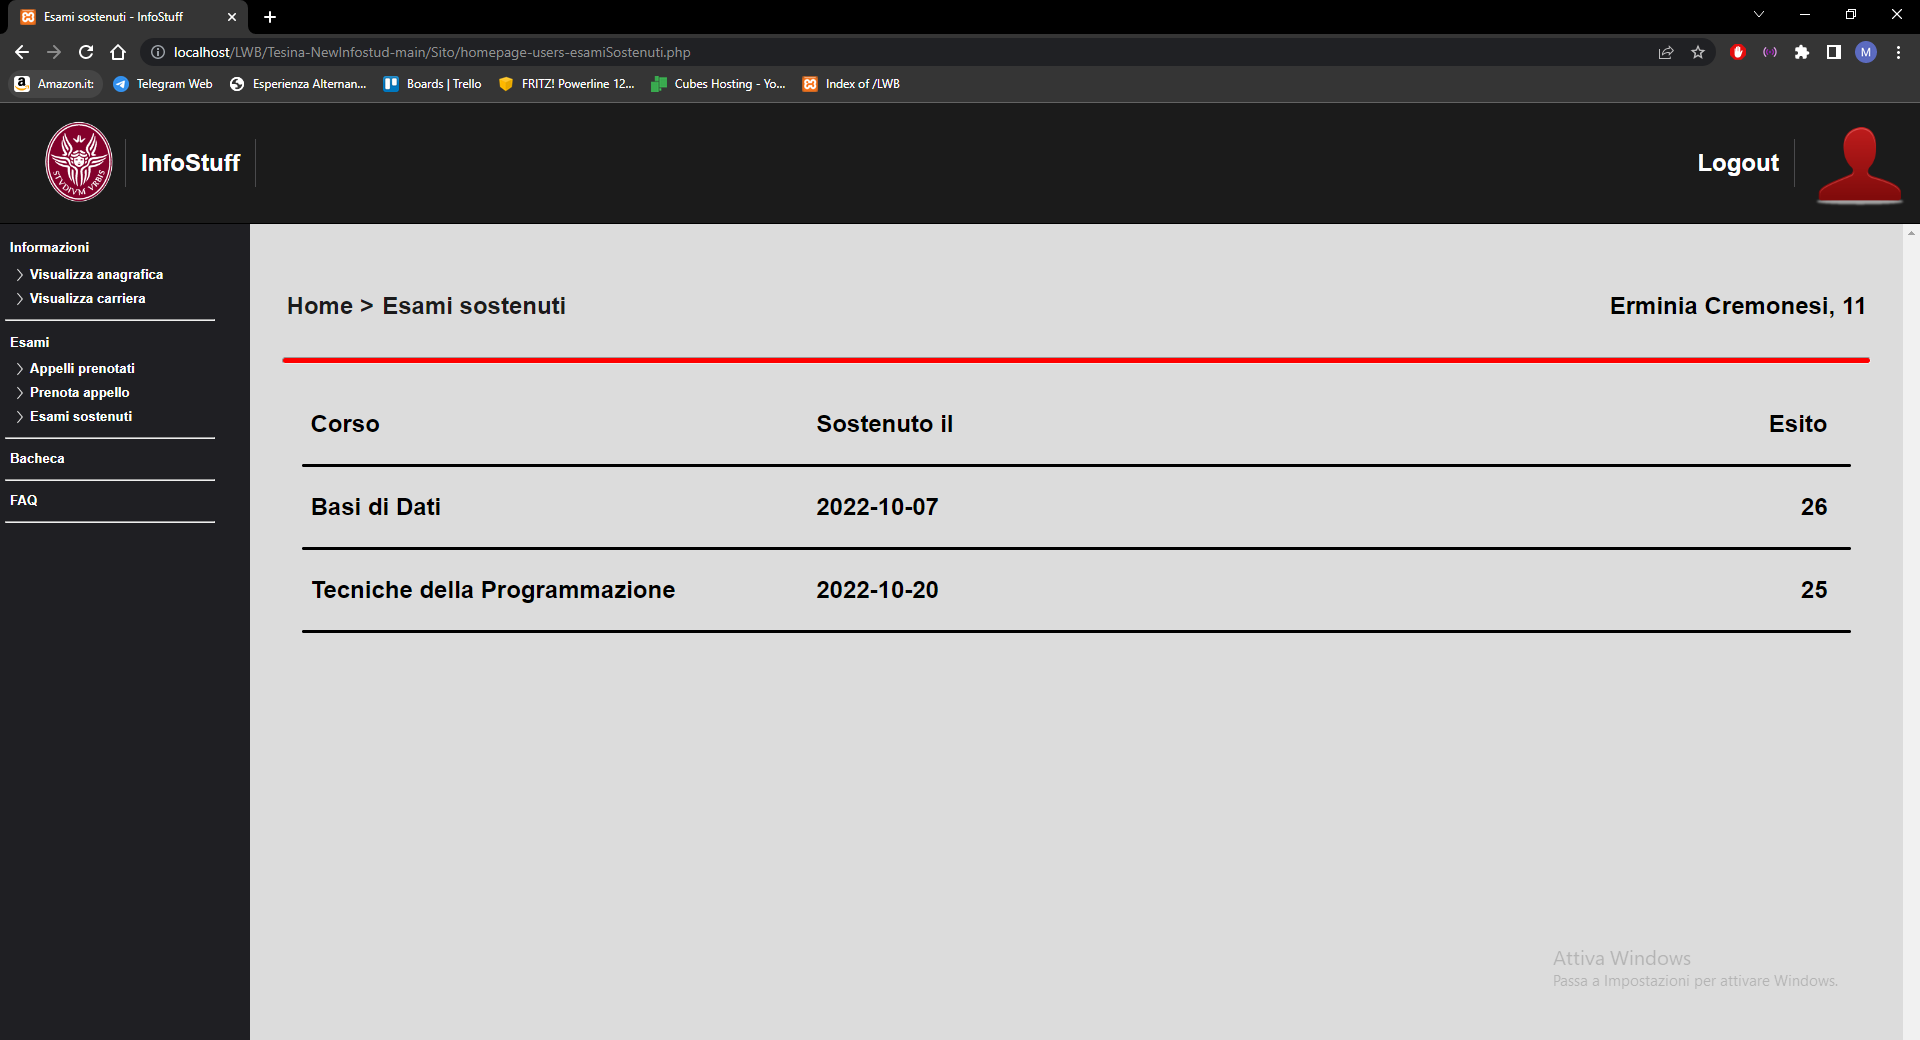
\includegraphics[scale=0.3]{figura2-13.png}
\caption{Pagina di visualizzazione dell'elenco degli esami sostenuti.}
\end{figure}

\medskip

\subsection{Prenotare gli appelli}

A partire da una qualsiasi pagina web relativa all'utenza, è possibile cliccare sulla voce \emph{Prenota appello}, sotto la sezione \emph{Esami}, all'interno della barra laterale sita a sinistra della pagina stessa. L'utente verrà così reindirizzato ad una pagina web come quella in figura 2.14, nella quale verranno mostrati tutti gli appelli che possono essere prenotati in quel momento; in particolare, verranno visualizzati tutti gli appelli che non sono stati prenotati e che non appartengono ad un esame per il quale esiste una verbalizzazione con esito positivo nel sistema. Interagendo con il blocco dell'esame, l'utente potrà quindi prenotarsi all'appello di suo interesse, tramite la pressione del bottone \emph{prenota}.

\begin{figure}
\centering
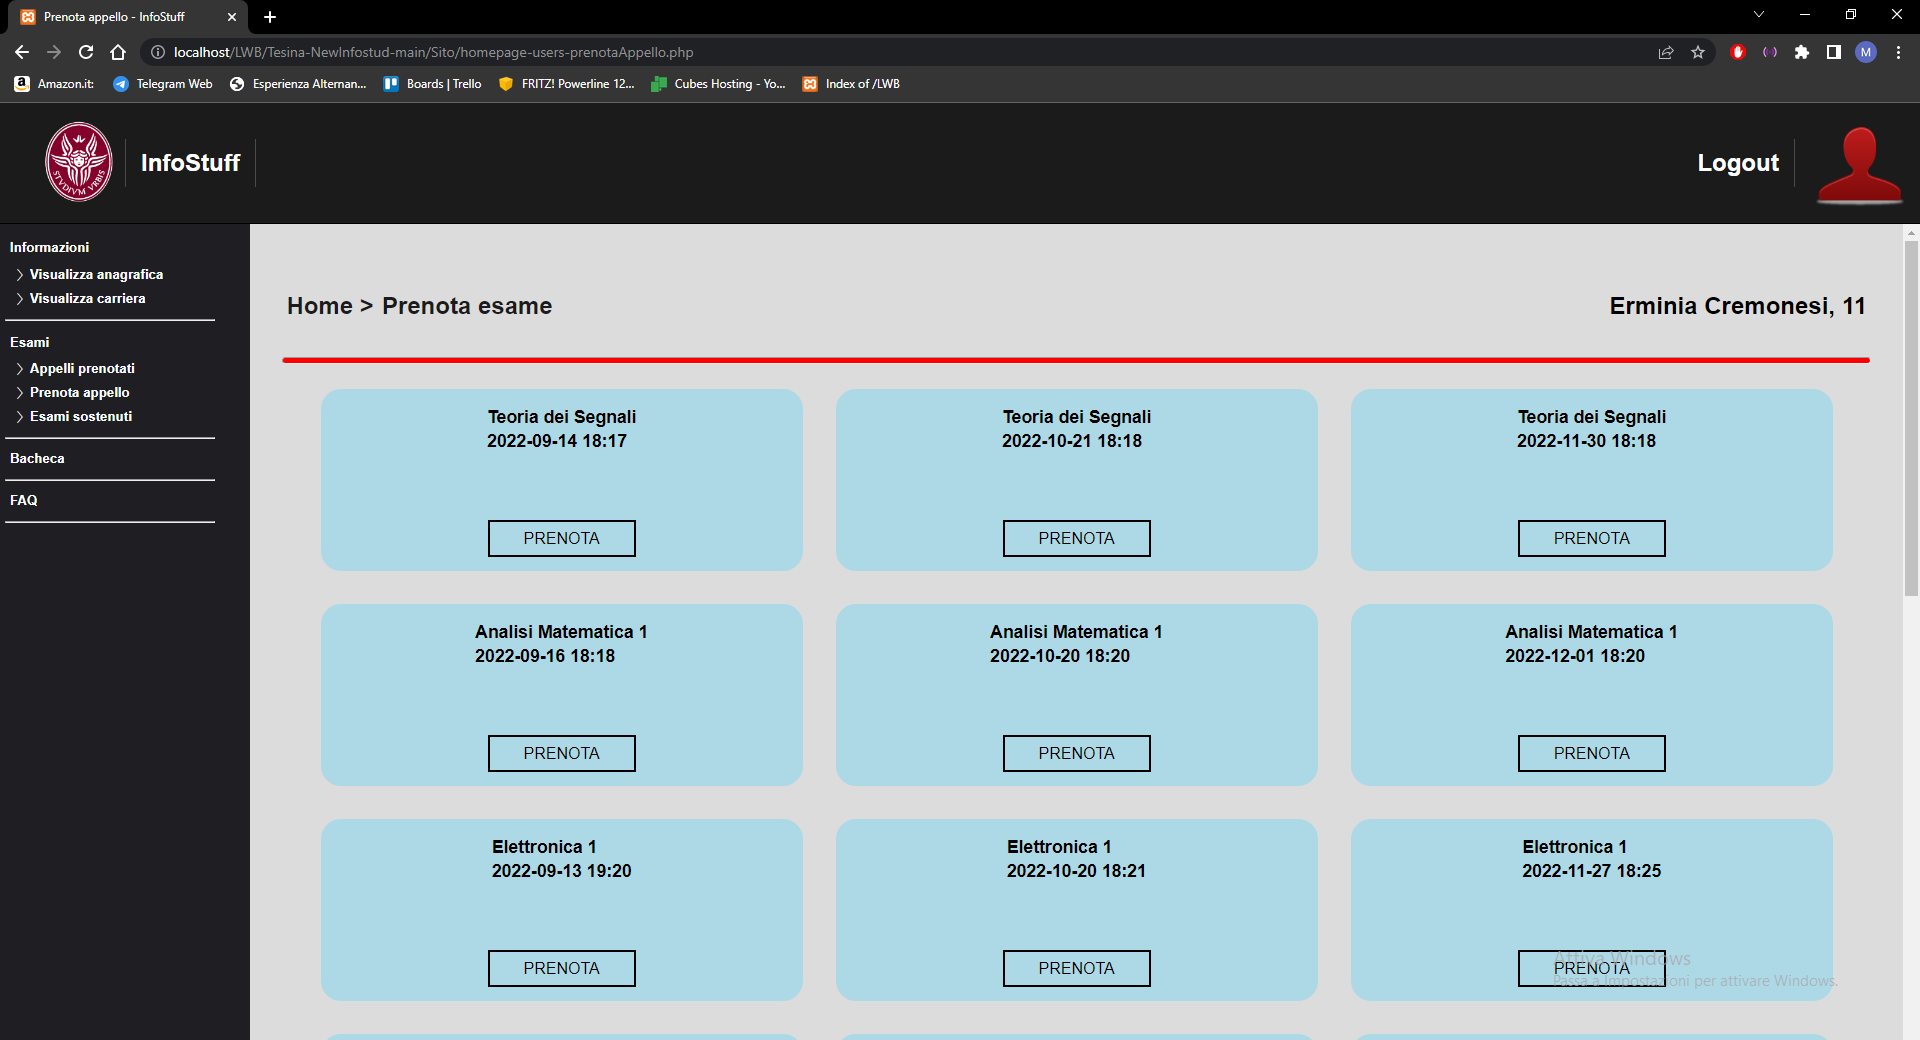
\includegraphics[scale=0.3]{figura2-14.png}
\caption{Pagina di prenotazione di un appello.}
\end{figure}

\medskip

\subsection{Accedere alle bacheche}

La fruizione delle bacheche è un'importante ed innovativa funzionalità offerta dalla piattaforma e si compone di diversi strumenti messi a disposizione allo studente, \textbf{purché non sia stato sospeso da un'utenza amministrativa}. A partire da una qualsiasi pagina web relativa all'utenza, è possibile cliccare sulla voce \emph{Bacheca}, all'interno della barra laterale sita a sinistra della pagina stessa. L'utente verrà così reindirizzato ad una pagina web come quella in figura 2.15, nella quale vengono elencati tutti i corsi appartenenti al corso di laurea cui lo studente autenticato nella sessione corrente risulta iscritto.

\begin{figure}
\centering
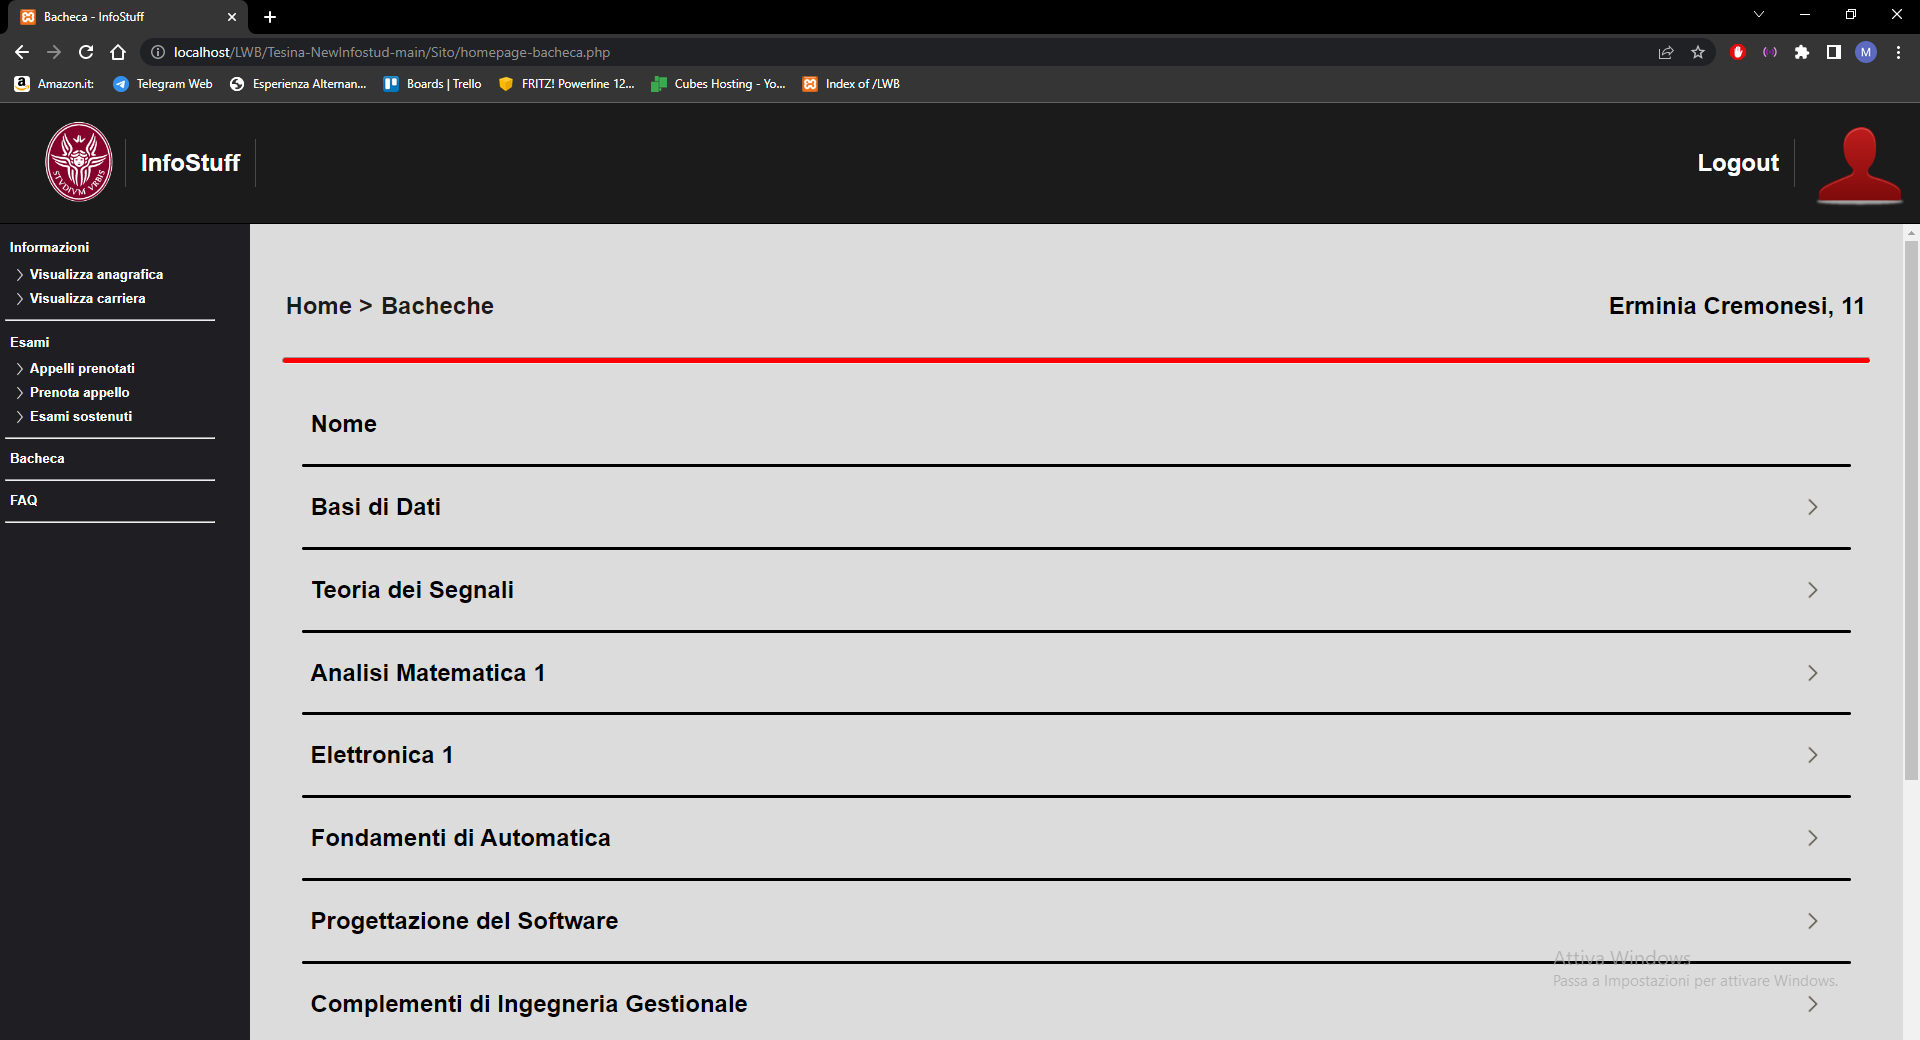
\includegraphics[scale=0.3]{figura2-15.png}
\caption{Lista dei corsi relativi al corso di laurea a cui lo studente autenticato è iscritto.}
\end{figure}

In questa pagina web, ciascuna voce rappresenta la bacheca dei singoli corsi. Interagendo con una di queste voci, l'utente viene reindirizzato ad una pagina web simile a quella mostrata in figura 2.16. La pagina in questione rappresenta una singola bacheca associata ad un determinato corso. Essa consiste di un menù di navigazione, posto nella parte superiore del corpo della bacheca, che consente all'utente di attraversare le diverse pagine della bacheca stessa (\emph{facciamo notare che il numero di post che possono essere visualizzati per pagina è pari a 5}). Sempre nella parte superiore, allo stesso livello del menù di navigazione, è presente un bottone \emph{crea post}, la cui pressione scatena un evento di creazione o di eliminazione di una form, posta al di sopra dell'elenco dei post (figura 2.17). Tramite questa form è possibile pubblicare un nuovo al post all'interno della bacheca.

\begin{figure}
\centering
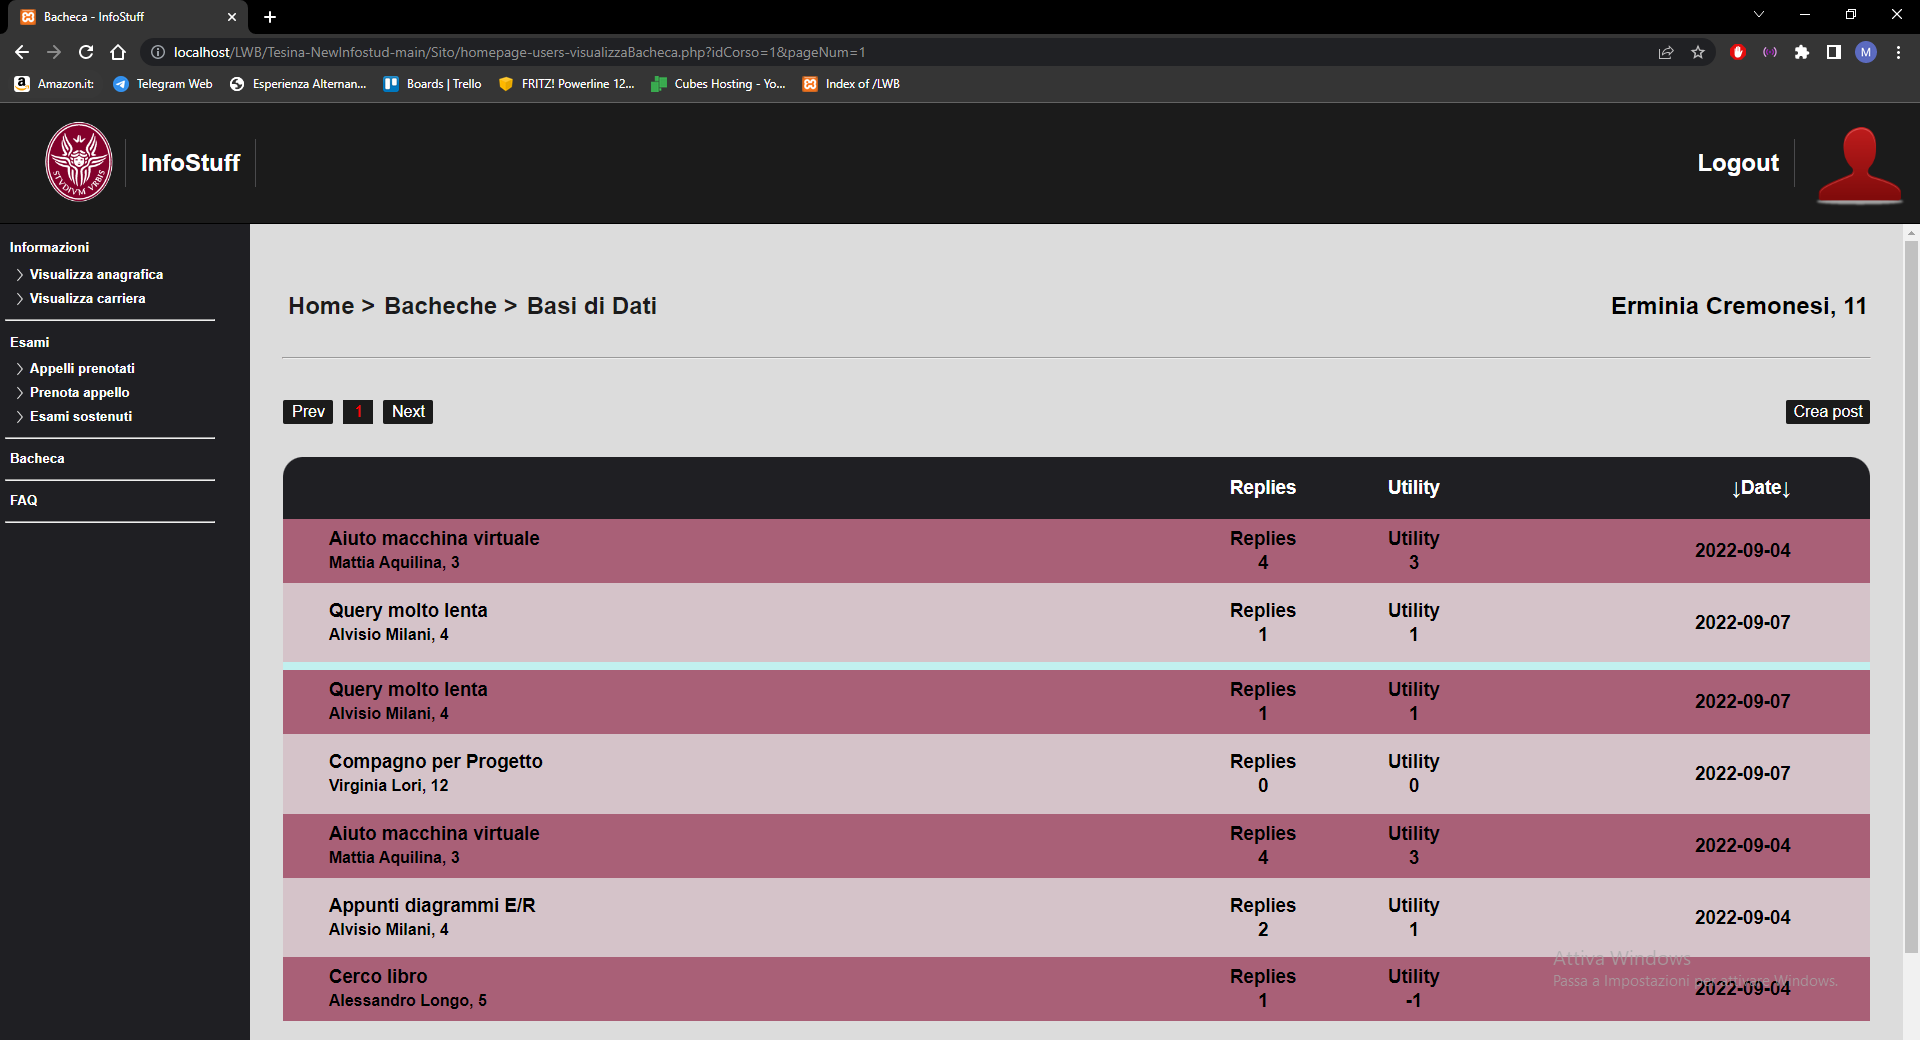
\includegraphics[scale=0.3]{figura2-16.png}
\caption{Bacheca di un singolo corso.}
\end{figure}

\begin{figure}
\centering
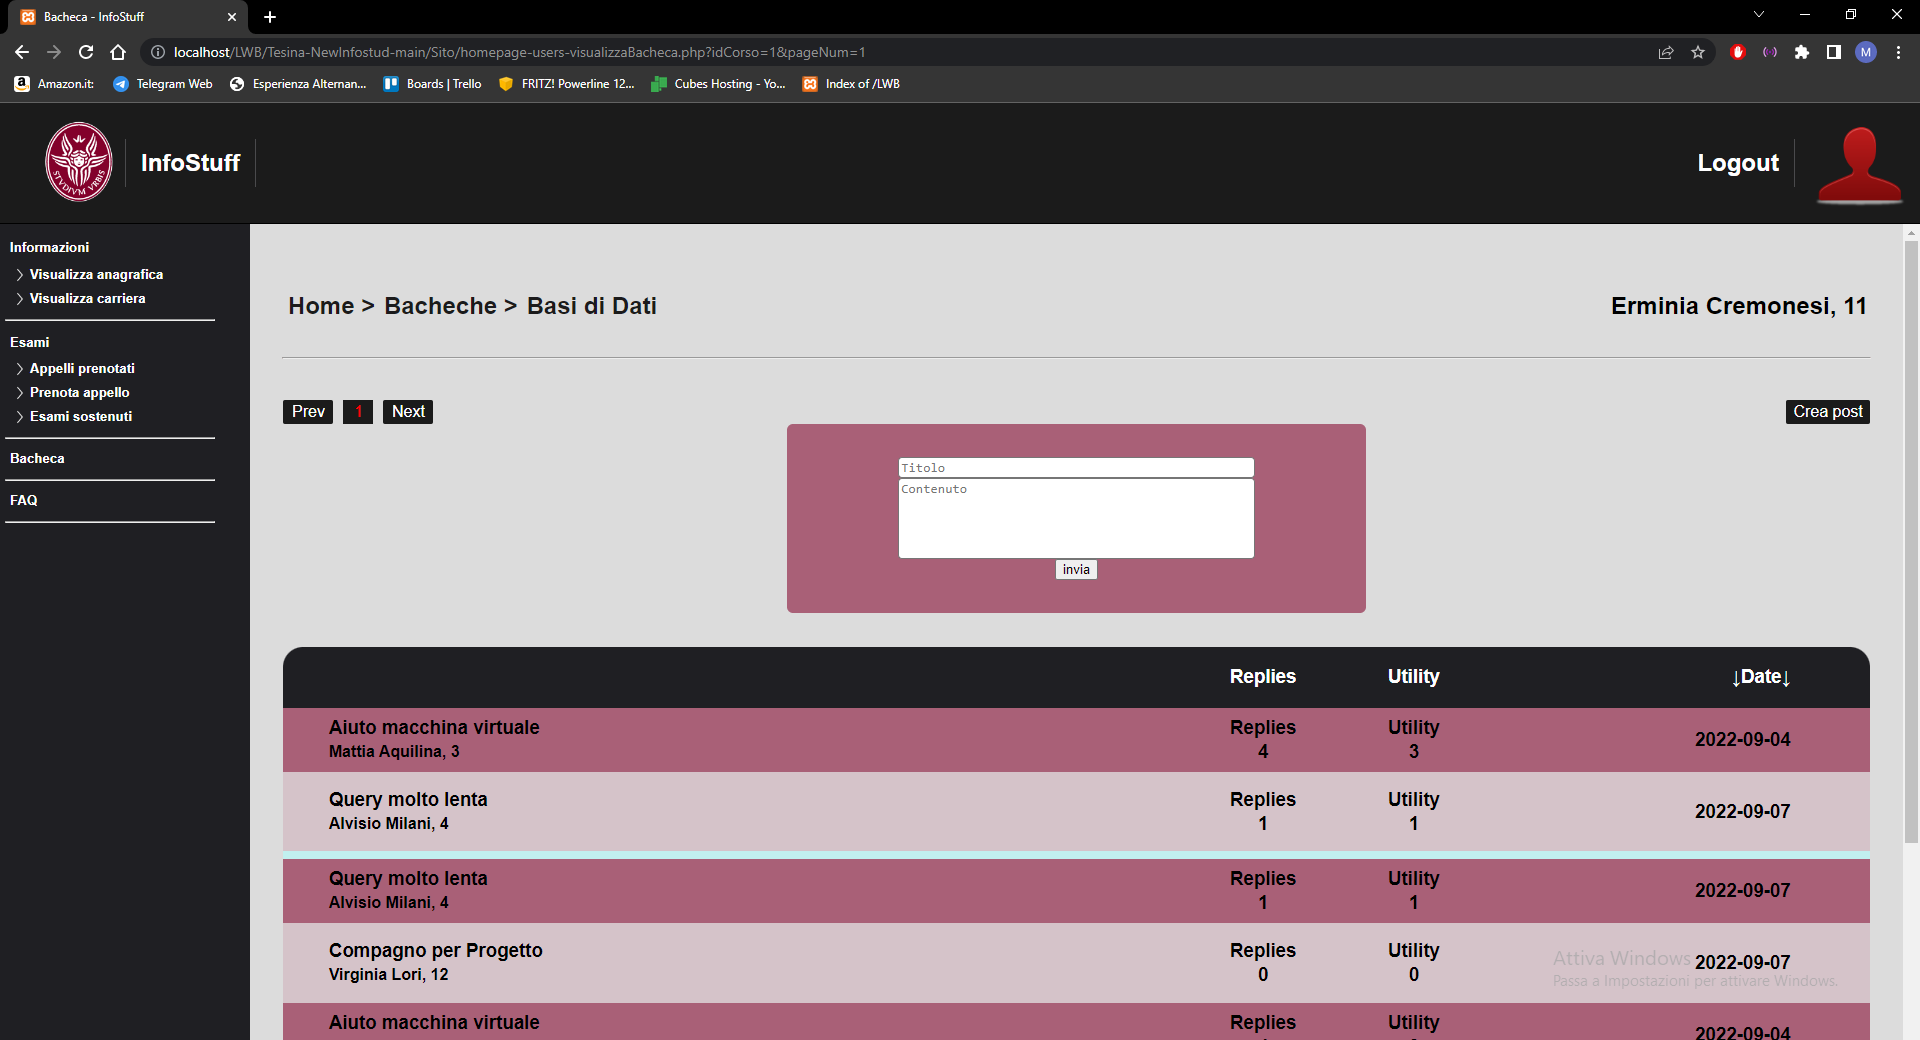
\includegraphics[scale=0.3]{figura2-17.png}
\caption{Bacheca con opzione di creazione di un post.}
\end{figure}

Nel blocco centrale della pagina web, troviamo l'elenco vero e proprio dei post relativi alla singola bacheca selezionata. In cima alla lista dei post è presente una barra orizzontale, che ci permette di applicare alcuni filtri di visualizzazione dei post sottostanti, fra i quali possiamo citare l'ordinamento sull'utilità dei post, sul numero di risposte ai singoli post e sulla data di pubblicazione dei singoli post. Inoltre, in ogni bacheca vengono sempre posti in sovraimpressione i due post che hanno ricevuto più voti utilità, e vengono separati dall'elenco tramite un separatore a forma di barra orizzontale celeste. Interagendo con una voce dell'elenco visualizzato, si raggiunge una pagina che visualizza il post scelto, la cui descrizione è contenuta nella sezione successiva.

\medskip

\subsubsection{Interagire con i post}

L'interazione con il post avviene in un'apposita pagina di visualizzazione del contenuto di quest'ultimo. Analizzando la schermata dall'alto (cfr. figura 2.18), troviamo innanzitutto l'intestazione del post, che si compone di una coppia di frecce, utilizzate per votare l'utilità del post stesso, e da un blocco contente autore, data di pubblicazione e contenuto di quest'ultimo. Qualora l'utenza correntemente autenticata fosse anche l'autore del post in visualizzazione, nell'angolo in alto a destra verrebbero visualizzate due icone, che permettono rispettivamente di eliminare il post e di modificarne il contenuto.

\begin{figure}
\centering
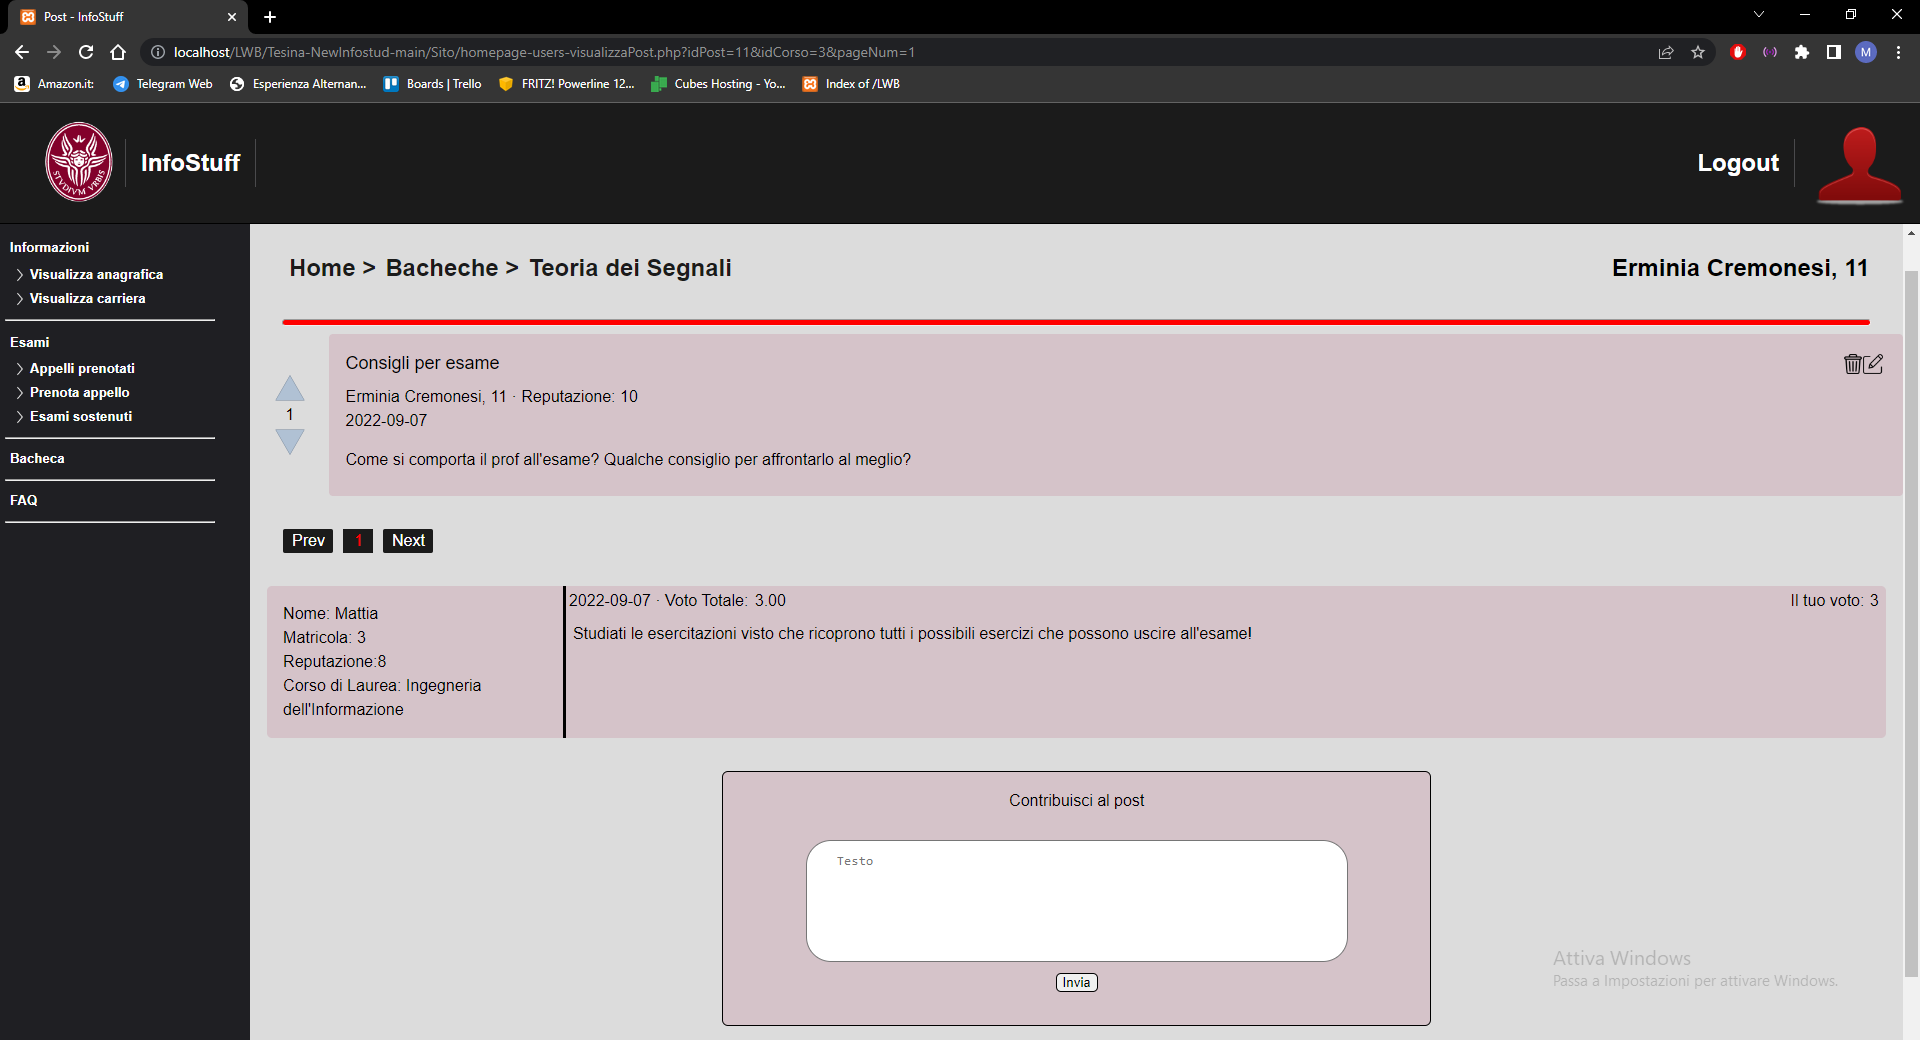
\includegraphics[scale=0.3]{figura2-18.png}
\caption{Pagina di visualizzazione di un post, con relativi commenti.}
\end{figure}

A seguire, verranno visualizzati in colonna tutti i commenti pubblicati in risposta al post, fino ad un massimo di cinque per pagina. Qualora il numero di commenti superasse questo limite, è sempre possibile interagire con la barra di navigazione contenuta tra il post e la lista dei commenti, per attraversare le diverse pagine. 

Ad un commento associamo due importanti funzionalità: quella di modifica/eliminazione, analoga a quelle dei post, e quella di voto. Nello specifico, un utente che non sia l'autore di un determinato commento, interagendo con la scritta \emph{il tuo voto} presente nell'angolo in alto a destra di blocco commento, attiverà un sistema di voto, graficamente rappresentato da cinque stelle: la pressione di una di queste ultime indicherà il grado di accordo dell'utente in relazione al commento votato.

Infine, ai piedi della pagina, troviamo una sezione che permette all'utente di pubblicare un commento relativo al post correntemente visualizzato nella pagina web.

\medskip

\textbf{\underline{Attenzione}}: ricordiamo al lettore che uno studente può accedere alla sezione delle bacheche dei propri corsi solo e soltanto se non è stato sospeso (\emph{soft ban}) da un'utenza amministrativa.

\medskip

\subsection{Accedere alle FAQ}

Il sistema delle FAQ permette agli studenti di interagire con i docenti proponendo delle domande in appositi box, o di votare quelle già presenti; saranno poi i docenti a scegliere le domande alle quali rispondere e le domande che possono essere eventualmente eliminate. A partire da una qualsiasi pagina web relativa all'utenza, è possibile cliccare sulla voce \emph{FAQ}, all'interno della barra laterale sita a sinistra della pagina stessa. L'utente, \textbf{a patto di non essere stato sospeso da un'utenza amministrativa}, alla pressione di tale pulsante verrà reindirizzato ad una pagina web come quella in figura 2.19, nella quale verrà presentata una lista dei corsi relativi al corso di laurea cui lo studente autenticato nella sessione corrente risulta essere iscritto; da qui, l'utente può scegliere un corso e, interagendo con l'apposito pulsante, può raggiungere la pagina delle FAQ specifica per il corso selezionato.

\begin{figure}
\centering
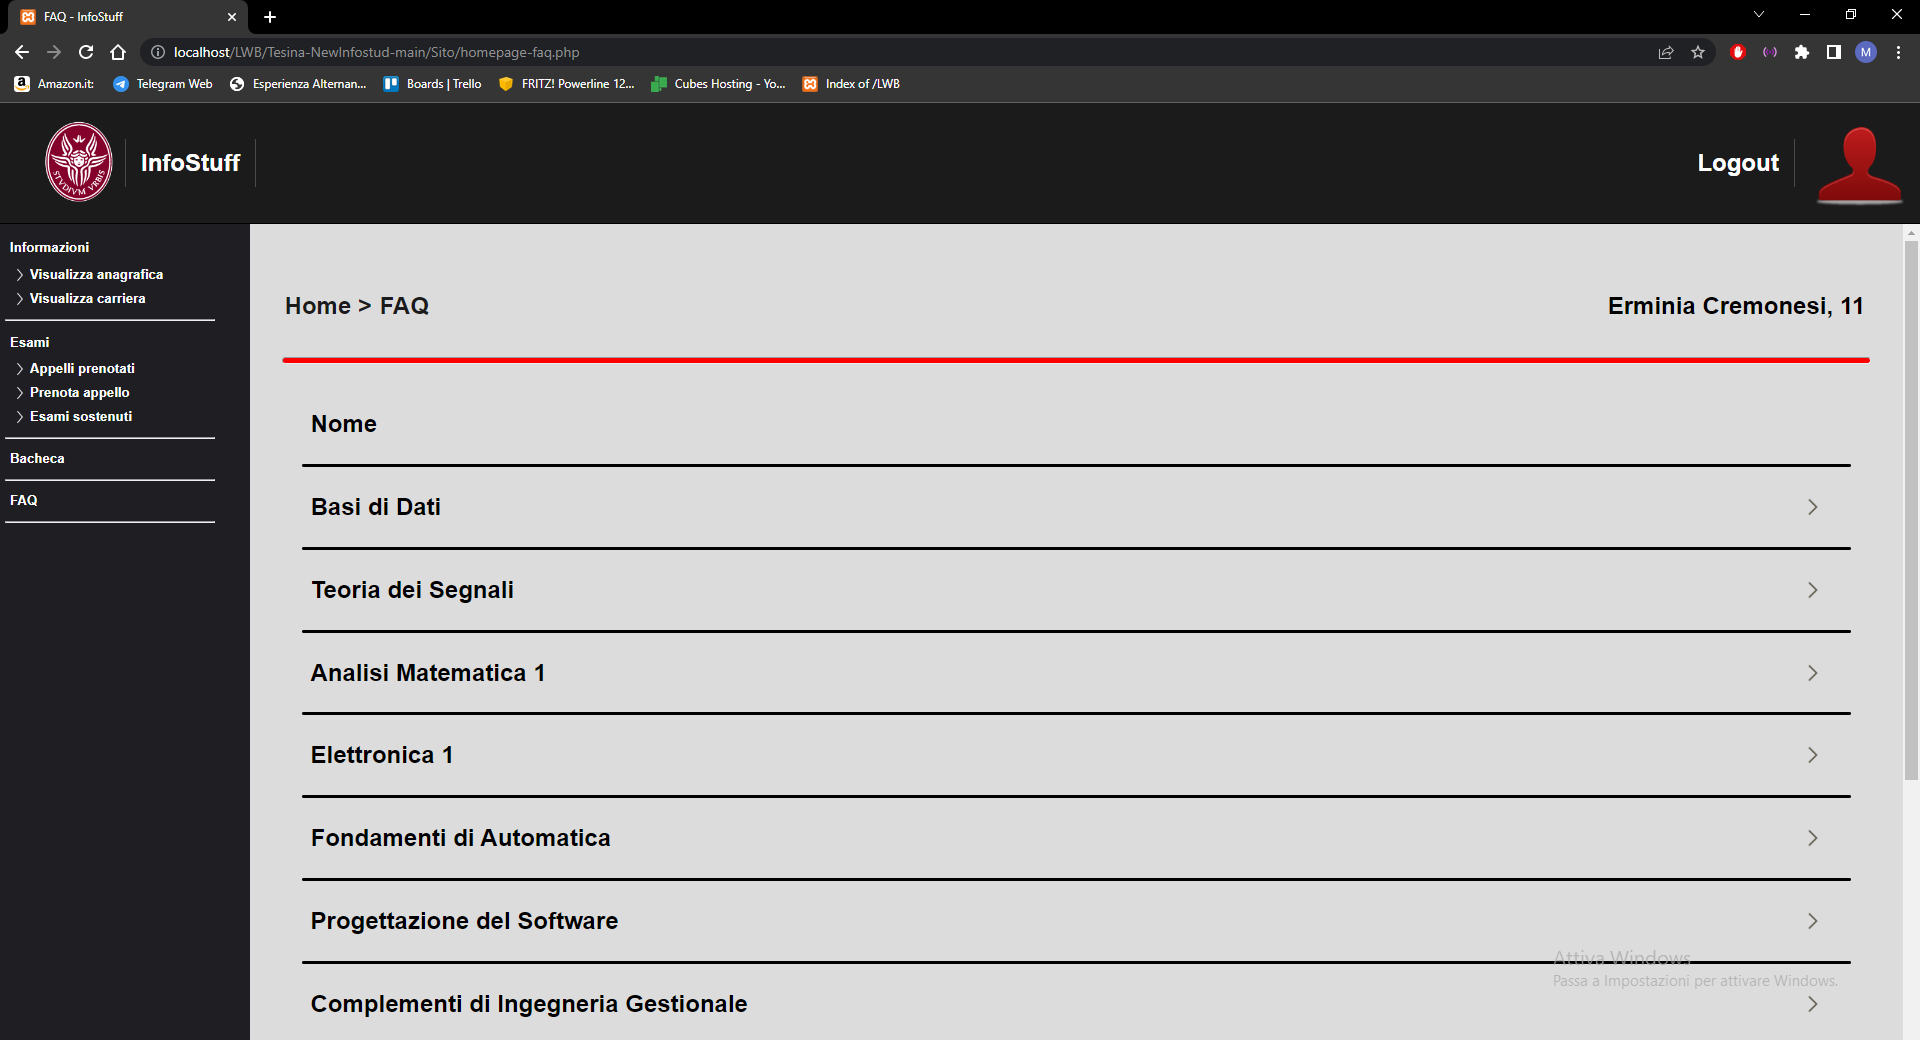
\includegraphics[scale=0.3]{figura2-19.png}
\caption{Lista dei corsi relativi al corso di laurea a cui lo studente autenticato è iscritto.}
\end{figure}

La pagina che si presenterà allo studente, mostrata in figura 2.20, è divisa in tre aree. In cima troviamo un box che rappresenta il contenitore di tutte quelle domande che hanno ricevuto una risposta. Il secondo blocco rappresenta invece il container delle domande ancora incomplete, ossia delle domande alle quali il docente non ha ancora pubblicato una risposta. Per una qualsiasi domanda, è possibile interagire con la coppia di frecce poste alla sinistra del testo, per esprimere un voto di utilità riguardante il contenuto della FAQ proposta. In fondo alla pagina, infine, troviamo una form che consente all'utente di contribuire alla FAQ, permettendogli di pubblicare una nuova domanda. 

\begin{figure}
\centering
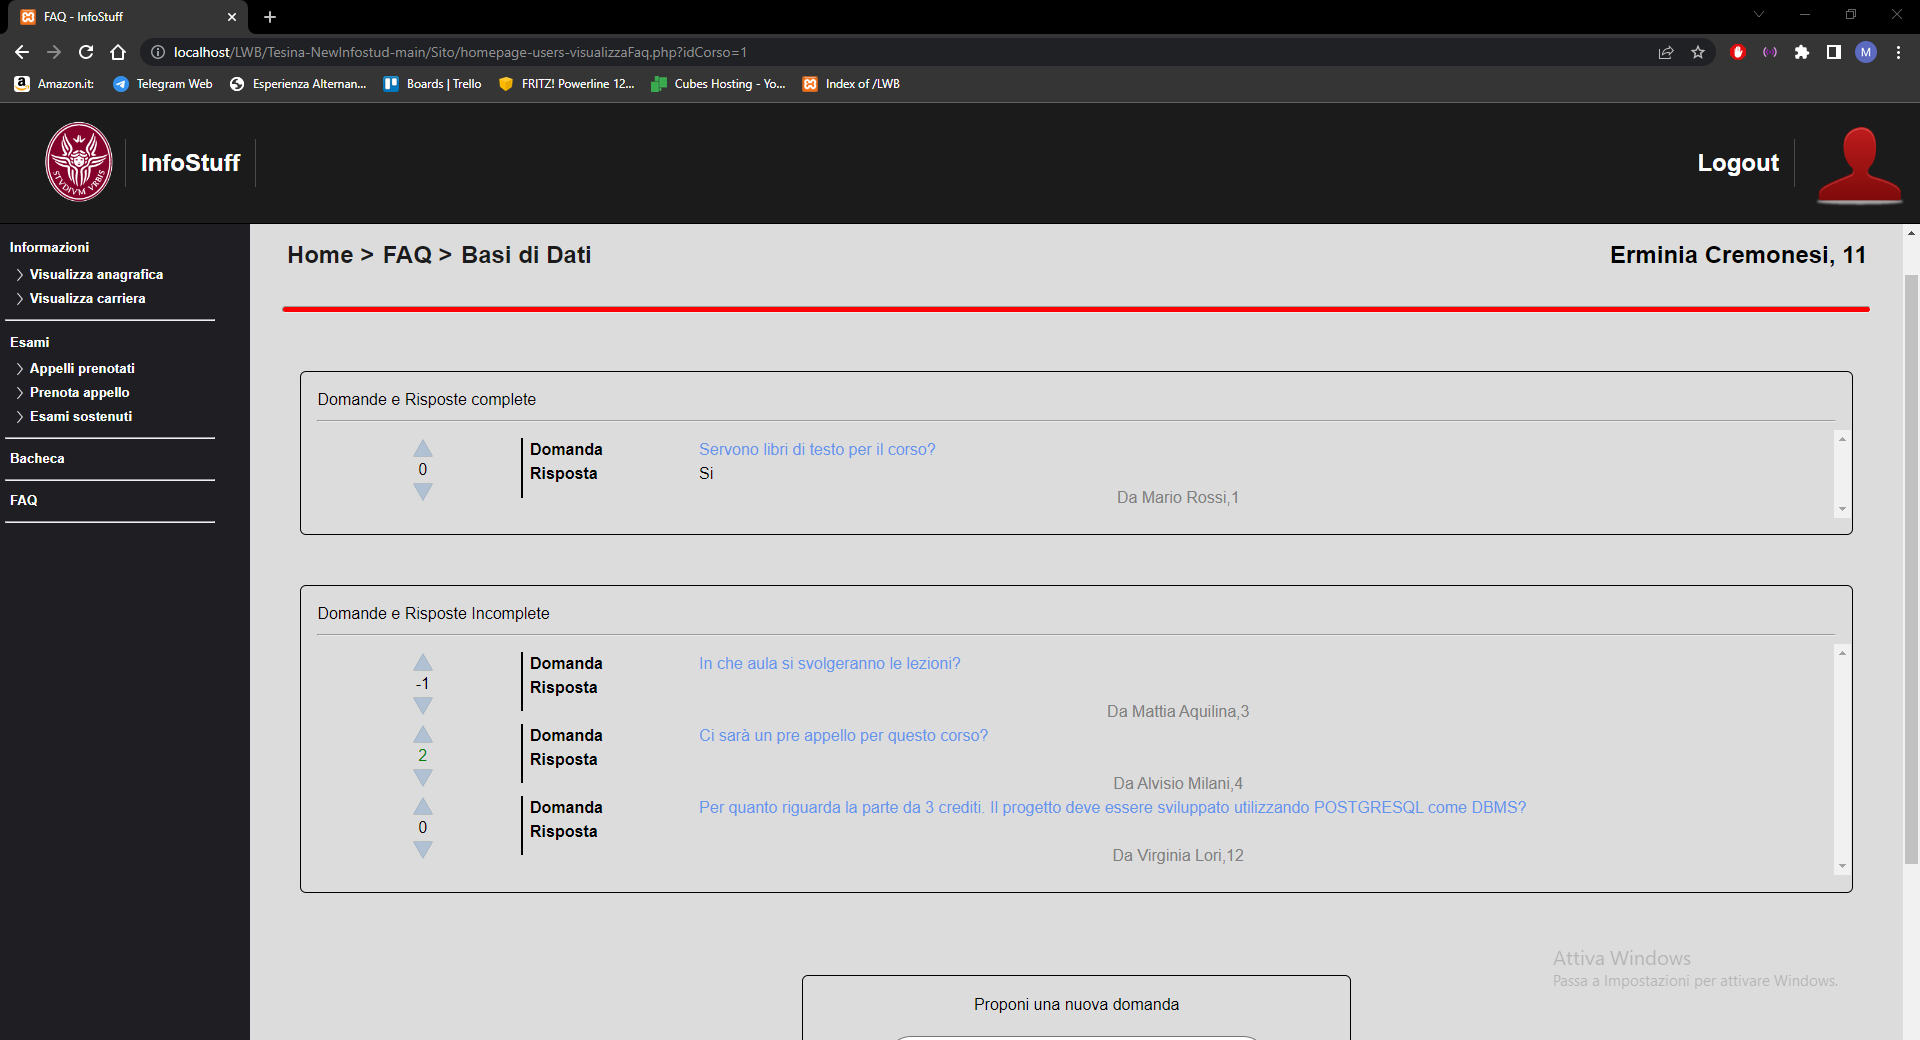
\includegraphics[scale=0.3]{figura2-20.png}
\caption{Pagina di visualizzazione della sezione FAQ relativa al corso selezionato.}
\end{figure}

\medskip

\textbf{\underline{Attenzione}}: ricordiamo al lettore che uno studente può accedere alla sezione delle FAQ dei propri corsi solo e soltanto se non è stato sospeso (\emph{soft ban}) da un'utenza amministrativa.

\medskip
\medskip

\section{Docente}

\subsection{Visualizzare l'anagrafica}

Una volta effettuato il login, ad un'utenza di tipologia \emph{Docente} verrà presentata una pagina web in cui saranno visualizzate le proprie informazioni anagrafiche, quali matricola, nome, cognome e password; quest'ultima verrà visualizzata coperta da degli asterischi, che rappresentano la lunghezza della relativa password criptata secondo l'algoritmo di cifratura MD5. Come per ogni altra utenza nella piattaforma, anche un docente può cambiare la propria password, premendo sull'apposita icona situata a fianco della password stessa (figura 2.21). 

\begin{figure}
\centering
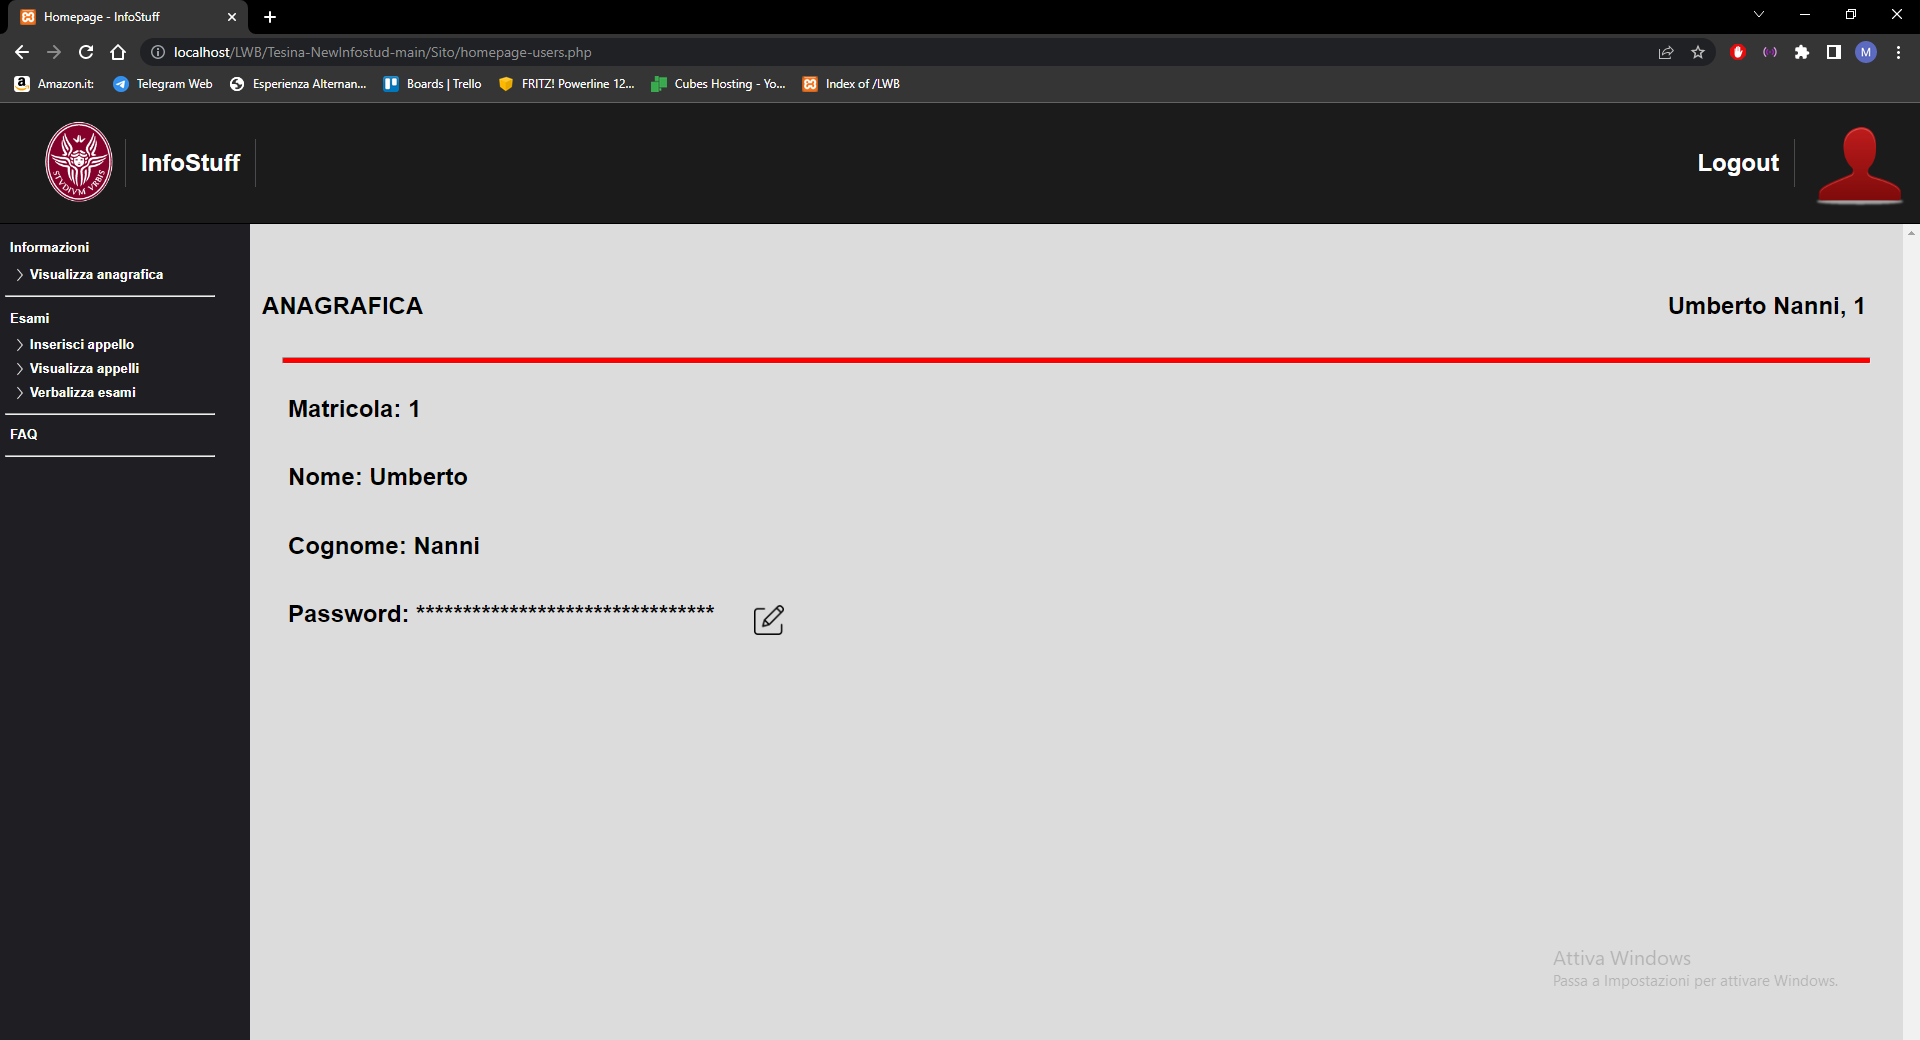
\includegraphics[scale=0.3]{figura2-21.png}
\caption{Homepage dell'utenza \emph{Docente}.}
\end{figure}

In questa homepage, inoltre, viene presentata una sidebar con tutte le funzionalità relative ai docenti, e che saranno descritte nel seguito di questo paragrafo. Si ricorda al lettore che, da qualsiasi pagina web del sito, è possibile tornare alla propria homepage di utenza cliccando sull'opportuna icona situata in alto a destra. Inoltre, da qualsiasi pagina web del sito, è possibile effettuare il logout: sarà sufficiente premere sull'apposito bottone sito anch'esso in alto a destra, a fianco dell'icona appena citata.

\medskip

\subsection{Visualizzare gli appelli}
\label{sec:visualizzaAppelli}

A partire da una qualsiasi pagina web relativa all'utenza, è possibile cliccare sulla voce \emph{Visualizza appelli}, sotto la sezione \emph{Esami}, all'interno della barra laterale sita a sinistra della pagina stessa. L'utente verrà così reindirizzato ad una pagina web come quella in figura 2.22, nella quale verranno presentati a schermo tutti gli appelli di tutti i corsi impartiti dal docente autenticato nella sessione corrente. In particolare, verranno visualizzati tutti gli appelli aventi data pari o successiva a quella corrente; la visualizzazione degli appelli è ordinata in base al seguente criterio: viene data la priorità all'ordinamento per nome del corso cui l'appello fa riferimento e, in seguito, gli appelli inerenti allo stesso corso vengono visualizzati in ordine cronologico.

\begin{figure}
\centering
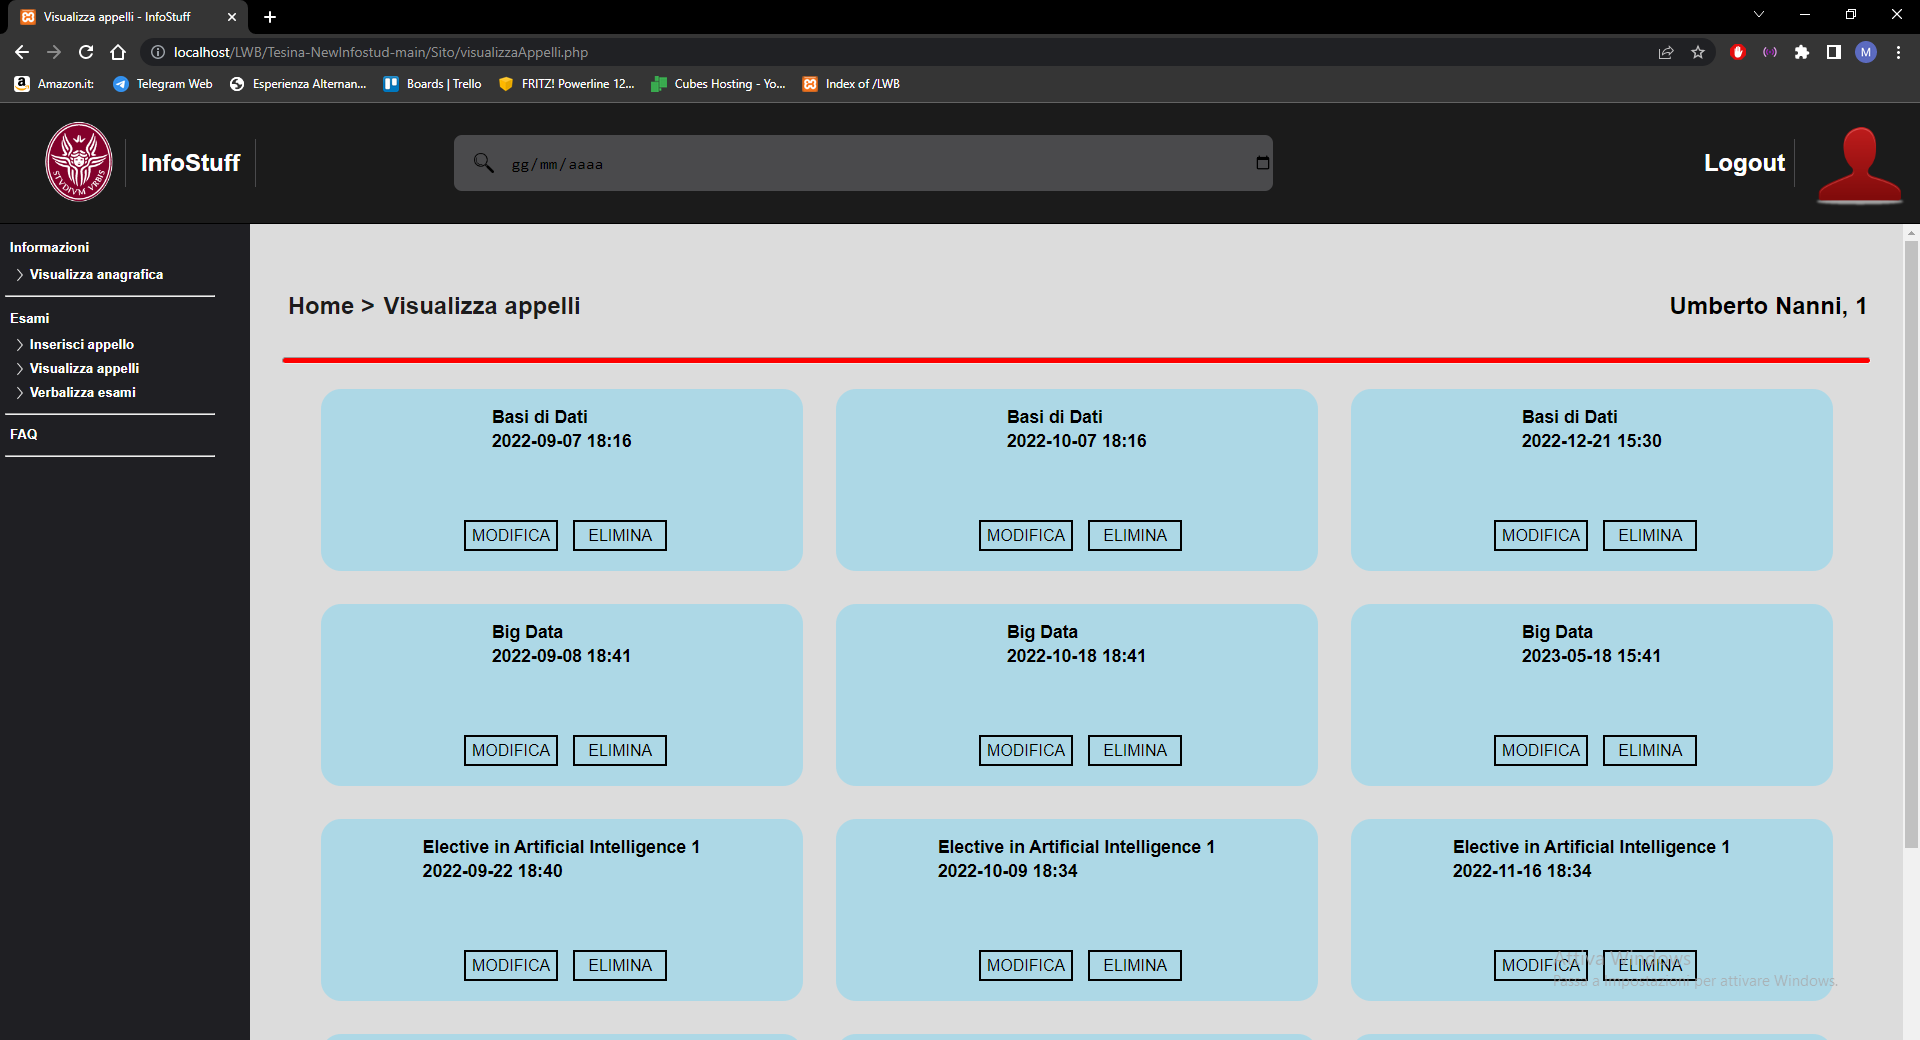
\includegraphics[scale=0.3]{figura2-22.png}
\caption{Visualizzazione degli appelli.}
\end{figure}

Il docente, a questo punto, dispone di tre scelte: può modificare un singolo appello, può eliminare un singolo appello, oppure può effettuare una ricerca di un appello mediante l'apposita barra di ricerca. La ricerca avviene tramite un meccanismo basato sulla data: in seguito alla ricerca, verranno visualizzati tutti gli appelli avente data pari o successiva a quella inserita.

\medskip

\subsubsection{Modificare un appello}

A partire dalla pagina di visualizzazione degli appelli, un docente può decidere di modificare un singolo appello: sarà sufficiente cliccare sull'apposito bottone \emph{modifica}, che si trova in corrispondenza dell'appello stesso, come mostrato in figura 2.22. La pressione di questo bottone porterà l'utente in una nuova pagina web, contenente una form di modifica dell'appello: i campi della form, come mostra la figura 2.23, sono già compilati con i dati dell'appello dal quale si proviene. L'utente sarà dunque libero di modificare i dati dell'appello a proprio piacimento; cliccando su \emph{invio}, l'appello verrà generalmente modificato. Tuttavia, in caso di corrispondenze con altri appelli, prima che la modifica venga effettuata, verrà mostrata all'utente una pagina web di segnalazione della corrispondenza avvenuta, come mostrato in figura 2.24. Le corrispondenze saranno approfondite in seguito, nel paragrafo relativo all'inserimento degli appelli.

\begin{figure}
\centering
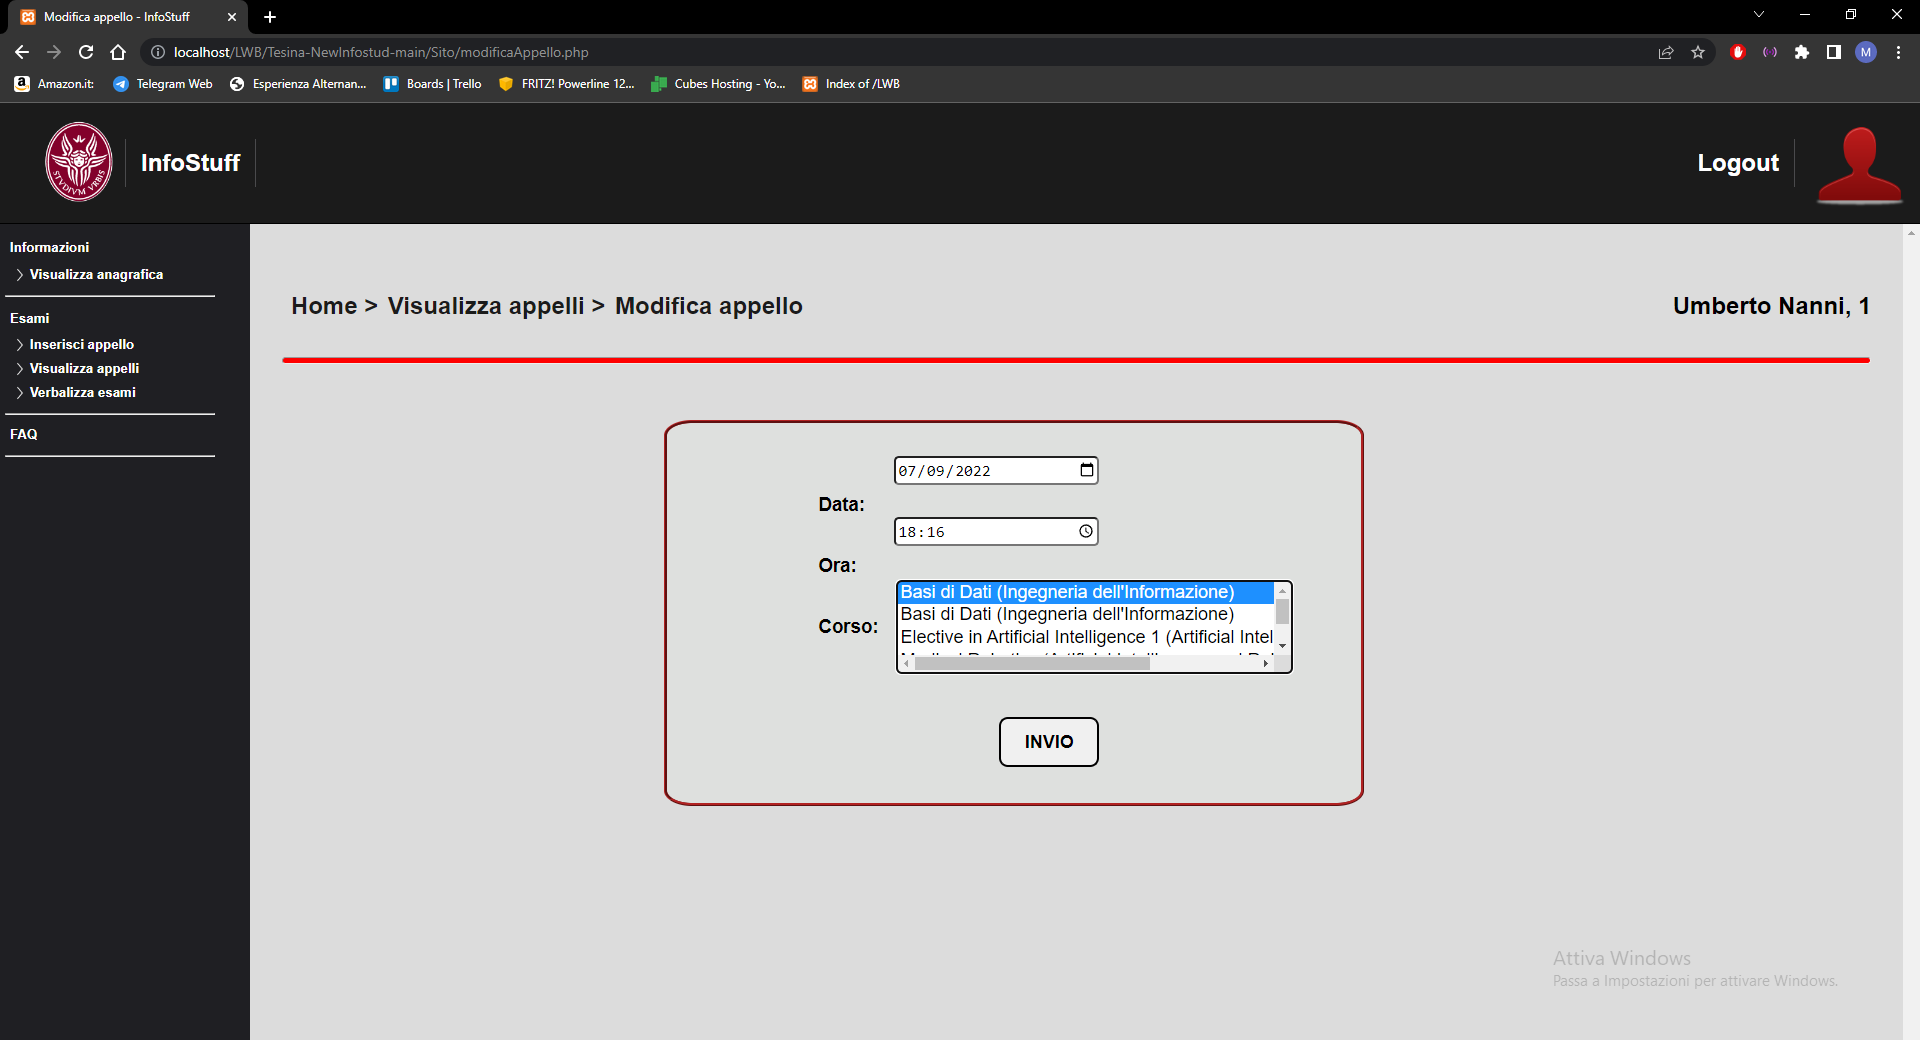
\includegraphics[scale=0.3]{figura2-23.png}
\caption{Form di modifica di un appello.}
\end{figure}

\begin{figure}
\centering
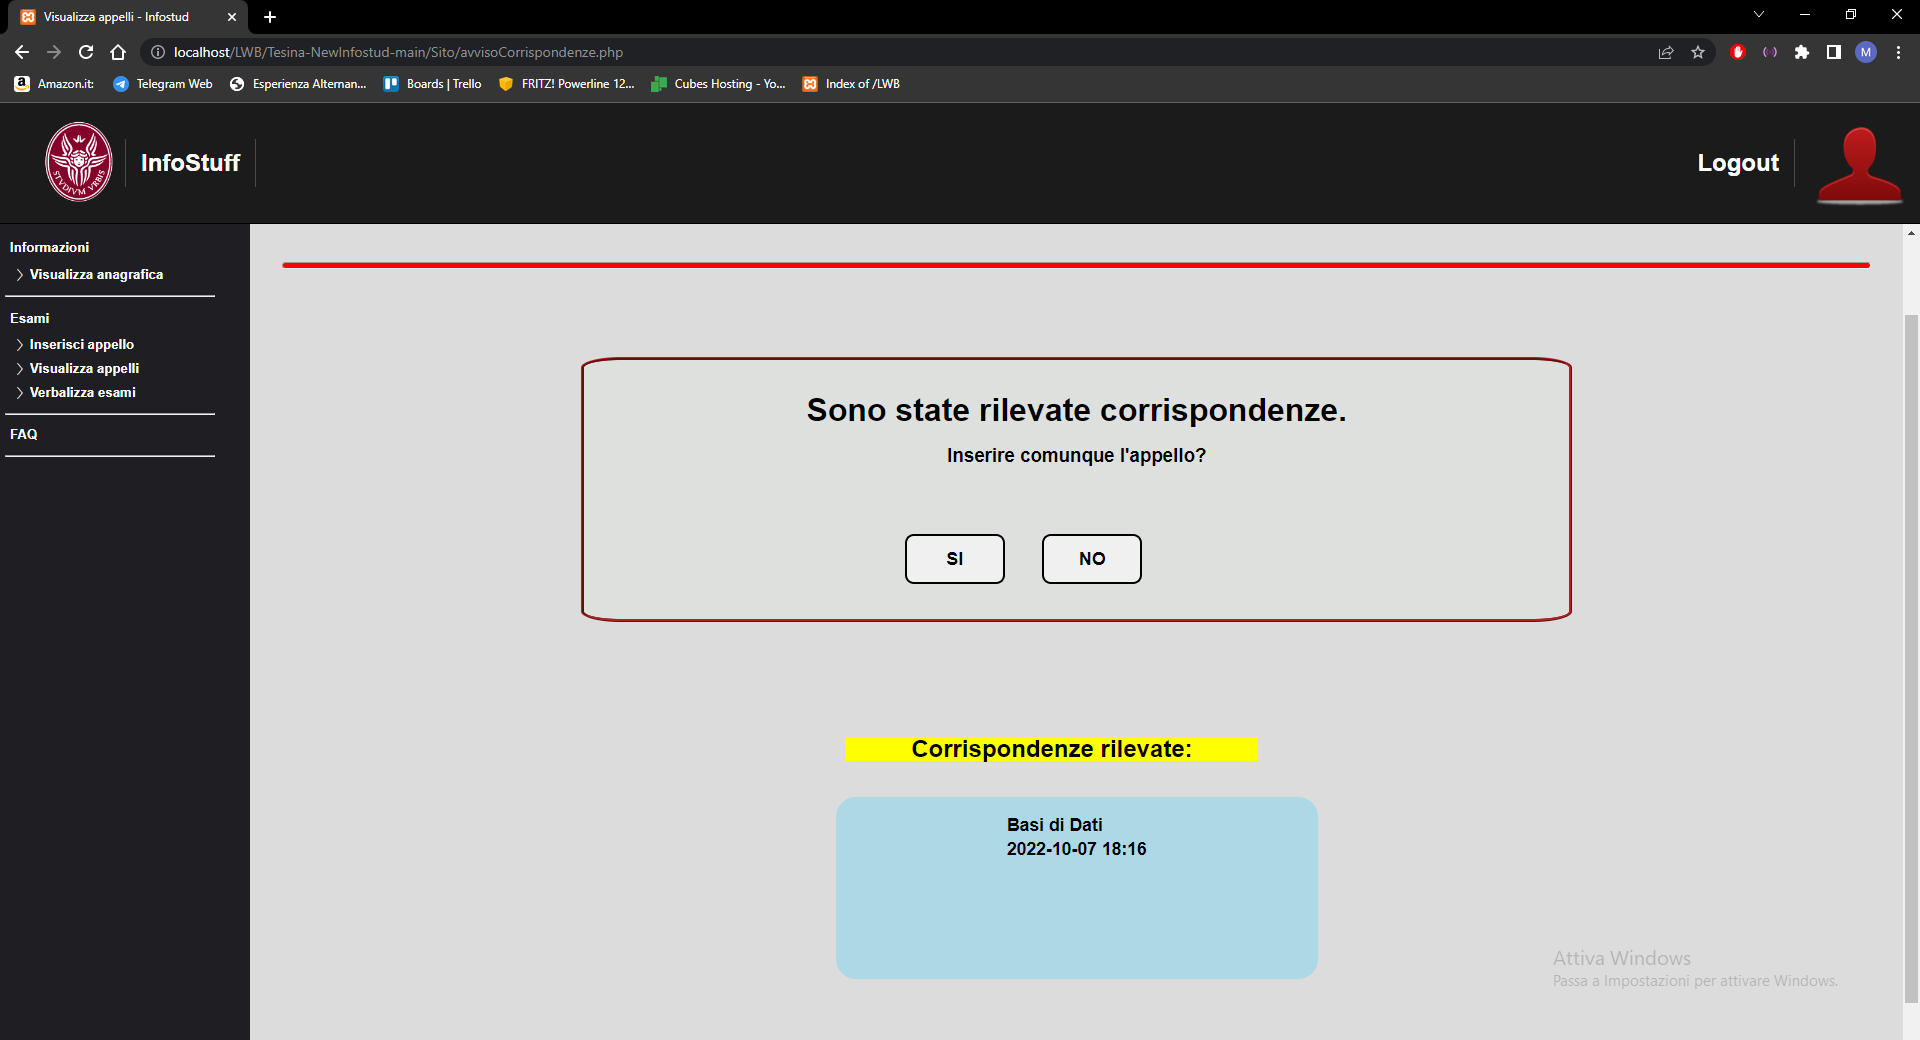
\includegraphics[scale=0.3]{figura2-24.png}
\caption{Visualizzazione delle corrispondenze.}
\end{figure}

In ogni caso, l'avvenuta modifica verrà segnalata da un opportuno avviso di successo; dualmente, in caso di errore, l'utente riceverà un'opportuna segnalazione.

\medskip

\subsubsection{Eliminare un appello}

A partire dalla pagina di visualizzazione degli appelli, un docente può decidere di eliminare un singolo appello: sarà sufficiente cliccare sull'apposito bottone \emph{elimina}, che si trova in corrispondenza dell'appello stesso, come mostrato in figura 2.22. La pressione di questo pulsante scatenerà l'esecuzione di una funzione di eliminazione che, dopo una prima conferma da parte dell'utente, \emph{eliminerà} l'appello selezionato (per ulteriori approfondimenti sull'eliminazione, si faccia riferimento al capitolo 3).

L'avvenuta eliminazione verrà segnalata da un opportuno avviso di successo; dualmente, in caso di errore, l'utente riceverà un'opportuna segnalazione.

\medskip

\subsection{Inserire un appello}

A partire da una qualsiasi pagina web relativa all'utenza, è possibile cliccare sulla voce \emph{Inserisci appello}, sotto la sezione \emph{Esami}, all'interno della barra laterale sita a sinistra della pagina stessa. L'utente verrà così reindirizzato ad una pagina web come quella in figura 2.25, nella quale verrà presentata a schermo una form per l'inserimento di un nuovo appello. L'utente potrà dunque scegliere una qualsiasi data, purché successiva a quella corrente, un qualsiasi orario e uno dei corsi di propria competenza; tutte queste informazioni sono obbligatorie. Premendo poi il pulsante \emph{invio}, le informazioni inserite andranno a costituire un nuovo appello, a meno di \textbf{collisioni}. L'utente potrà verificare l'avvenuto inserimento del nuovo appello mediante l'apposita funzionalità di visualizzazione degli appelli, trattata poc'anzi \hyperref[sec:visualizzaAppelli]{\textcolor{gray}{[$\uparrow$]}}.

\begin{figure}
\centering
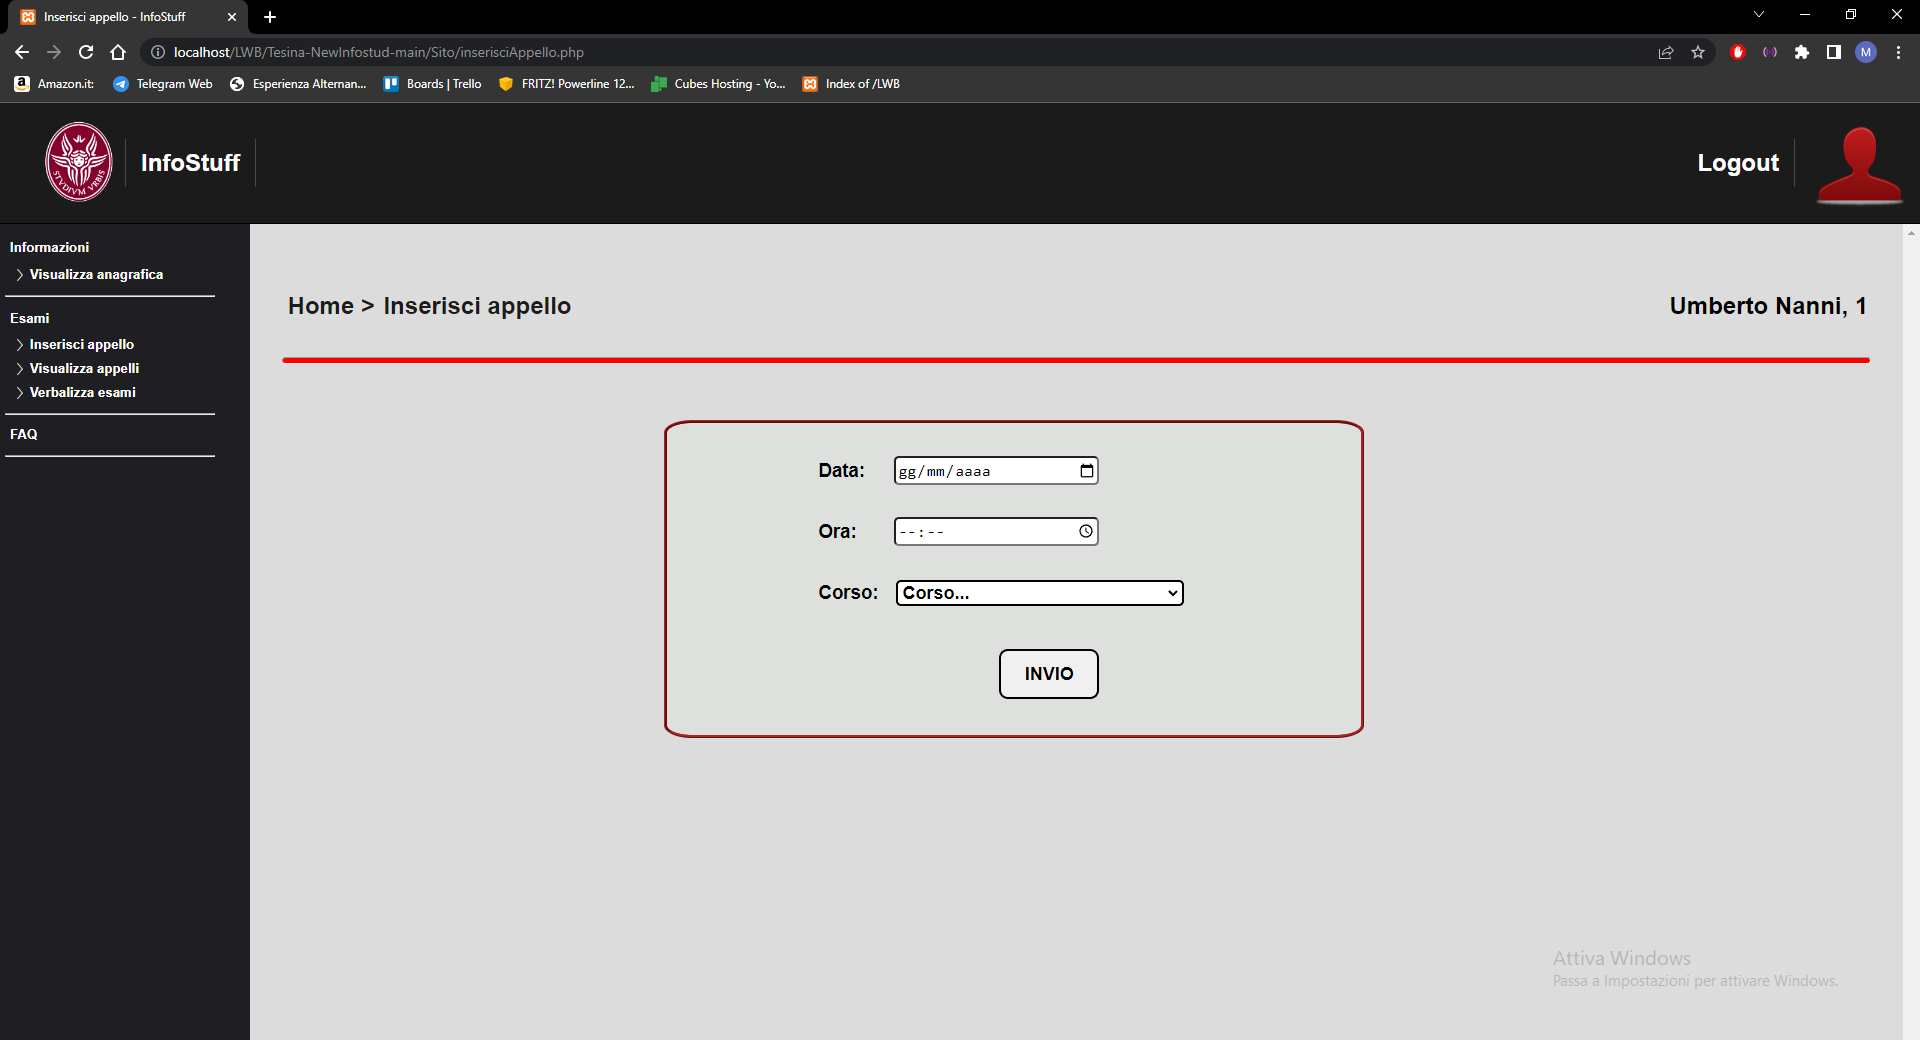
\includegraphics[scale=0.3]{figura2-25.png}
\caption{Form di inserimento di un appello.}
\end{figure}

Inserendo un appello in prossimità di altri appelli relativi a corsi di uno stesso anno inerenti ad uno stesso corso di laurea, si avrà una \emph{corrispondenza}. In occorrenza di tale evento, prima che avvenga l'effettivo inserimento (o l'effettiva modifica!) dell'appello in questione, l'utente verrà reindirizzato verso una pagina web in cui viene segnalata la presenza di corrispondenze, e in cui vengono presentate le corrispondenze rilevate, al fine di dar modo al docente di prendere la sua decisione sull'effettivo inserimento (o sull'effettiva modifica) dell'appello stesso. Come già citato, un'esemplificazione di una tale pagina web è riportata in figura 2.24. Rispondendo \emph{sì} alla domanda ''\emph{Sono state rilevate corrispondenze. Inserire comunque l'appello?}'', l'inserimento avverrà senza altri indugi; altrimenti, rispondendo \emph{no}, l'utente verrà reindirizzato alla pagina di inserimento (o di modifica) dell'appello, nella quale troverà la form già compilata con i dati precedentemente inseriti.

\medskip

\subsection{Verbalizzare gli esami}

A partire da una qualsiasi pagina web relativa all'utenza, è possibile cliccare sulla voce \emph{Verbalizza esami}, sotto la sezione \emph{Esami}, all'interno della barra laterale sita a sinistra della pagina stessa. L'utente verrà così reindirizzato ad una pagina web come quella in figura 2.26, nella quale verranno presentati a schermo tutti gli appelli di tutti i corsi impartiti dal docente autenticato nella sessione corrente. In particolare, verranno visualizzati tutti gli appelli aventi data pari o successiva a quella corrente; la visualizzazione degli appelli è ordinata in base al seguente criterio: viene data la priorità all'ordinamento per nome del corso cui l'appello fa riferimento e, in seguito, gli appelli inerenti allo stesso corso vengono visualizzati in ordine cronologico.

\begin{figure}
\centering
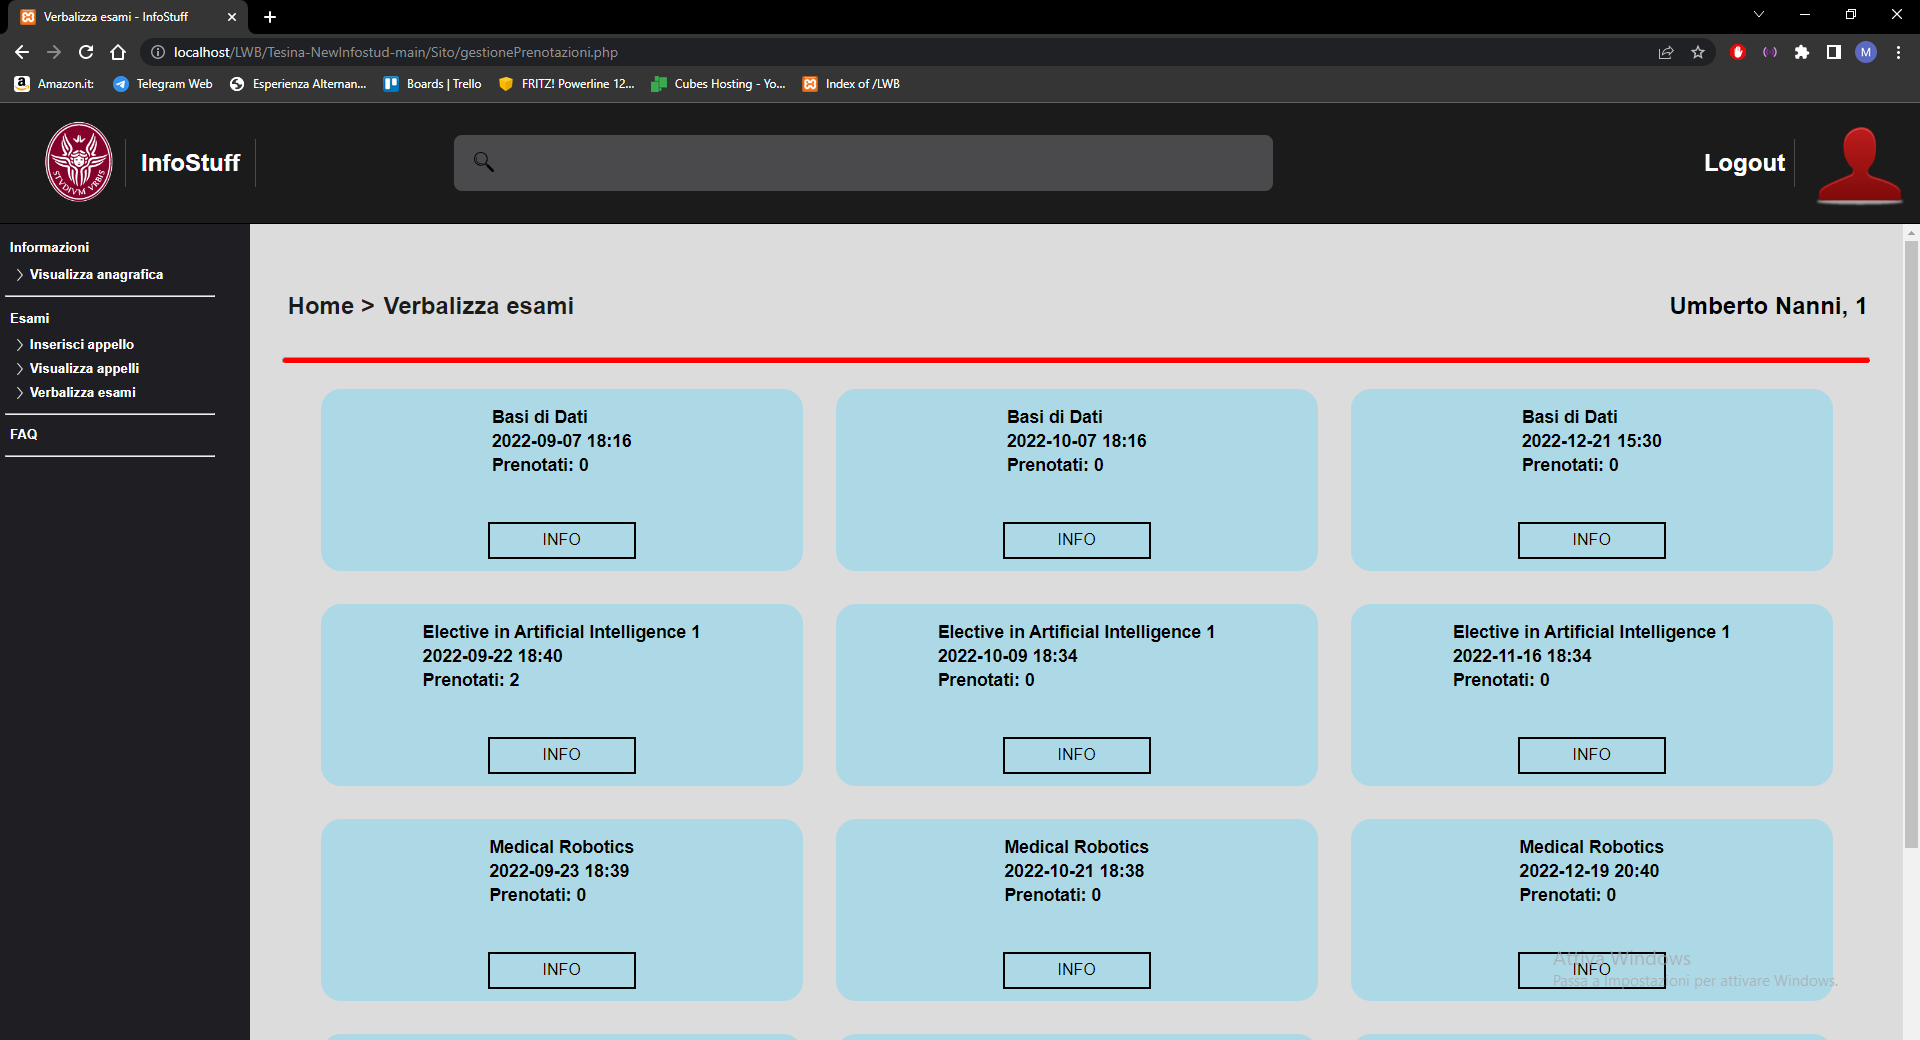
\includegraphics[scale=0.3]{figura2-26.png}
\caption{Pagina di visualizzazione degli appelli relativi ai corsi impartiti dal docente autenticato.}
\end{figure}

A differenza della semplice visualizzazione \hyperref[sec:visualizzaAppelli]{\textcolor{gray}{[$\uparrow$]}}, questa volta gli appelli vengono presentati con un'informazione aggiuntiva: il numero di studenti prenotati ai singoli appelli. Inoltre, come mostrato in figura 2.26, i singoli appelli dispongono di un pulsante \emph{info}, premendo il quale l'utente potrà accedere alla pagina web per l'effettiva verbalizzazione, mostrata in figura 2.27. Tale pagina avrà lo scopo di visualizzare una lista di tutti gli studenti iscritti all'appello selezionato; il docente potrà inserire la relativa valutazione nell'apposito campo \emph{esito} e, premendo sul pulsante \emph{verbalizza}, verrà effettuata la verbalizzazione di tutti gli esami aventi esito diverso da NULL. Come discusso nel capitolo 1 \hyperref[sec:specifiche]{\textcolor{gray}{[$\uparrow$]}}, l'esito di un esame verbalizzato può essere un numero compreso fra 18/30 e 30/30 con lode (il valore di un 30/30 con lode è pari a 31), oppure può essere una lettera, R o B; la lettera R indica il ritiro da parte dello studente dallo svolgimento dell'esame, mentre la lettera B indica una bocciatura, ossia la terminazione dell'esame svolto con esito negativo.

\begin{figure}
\centering
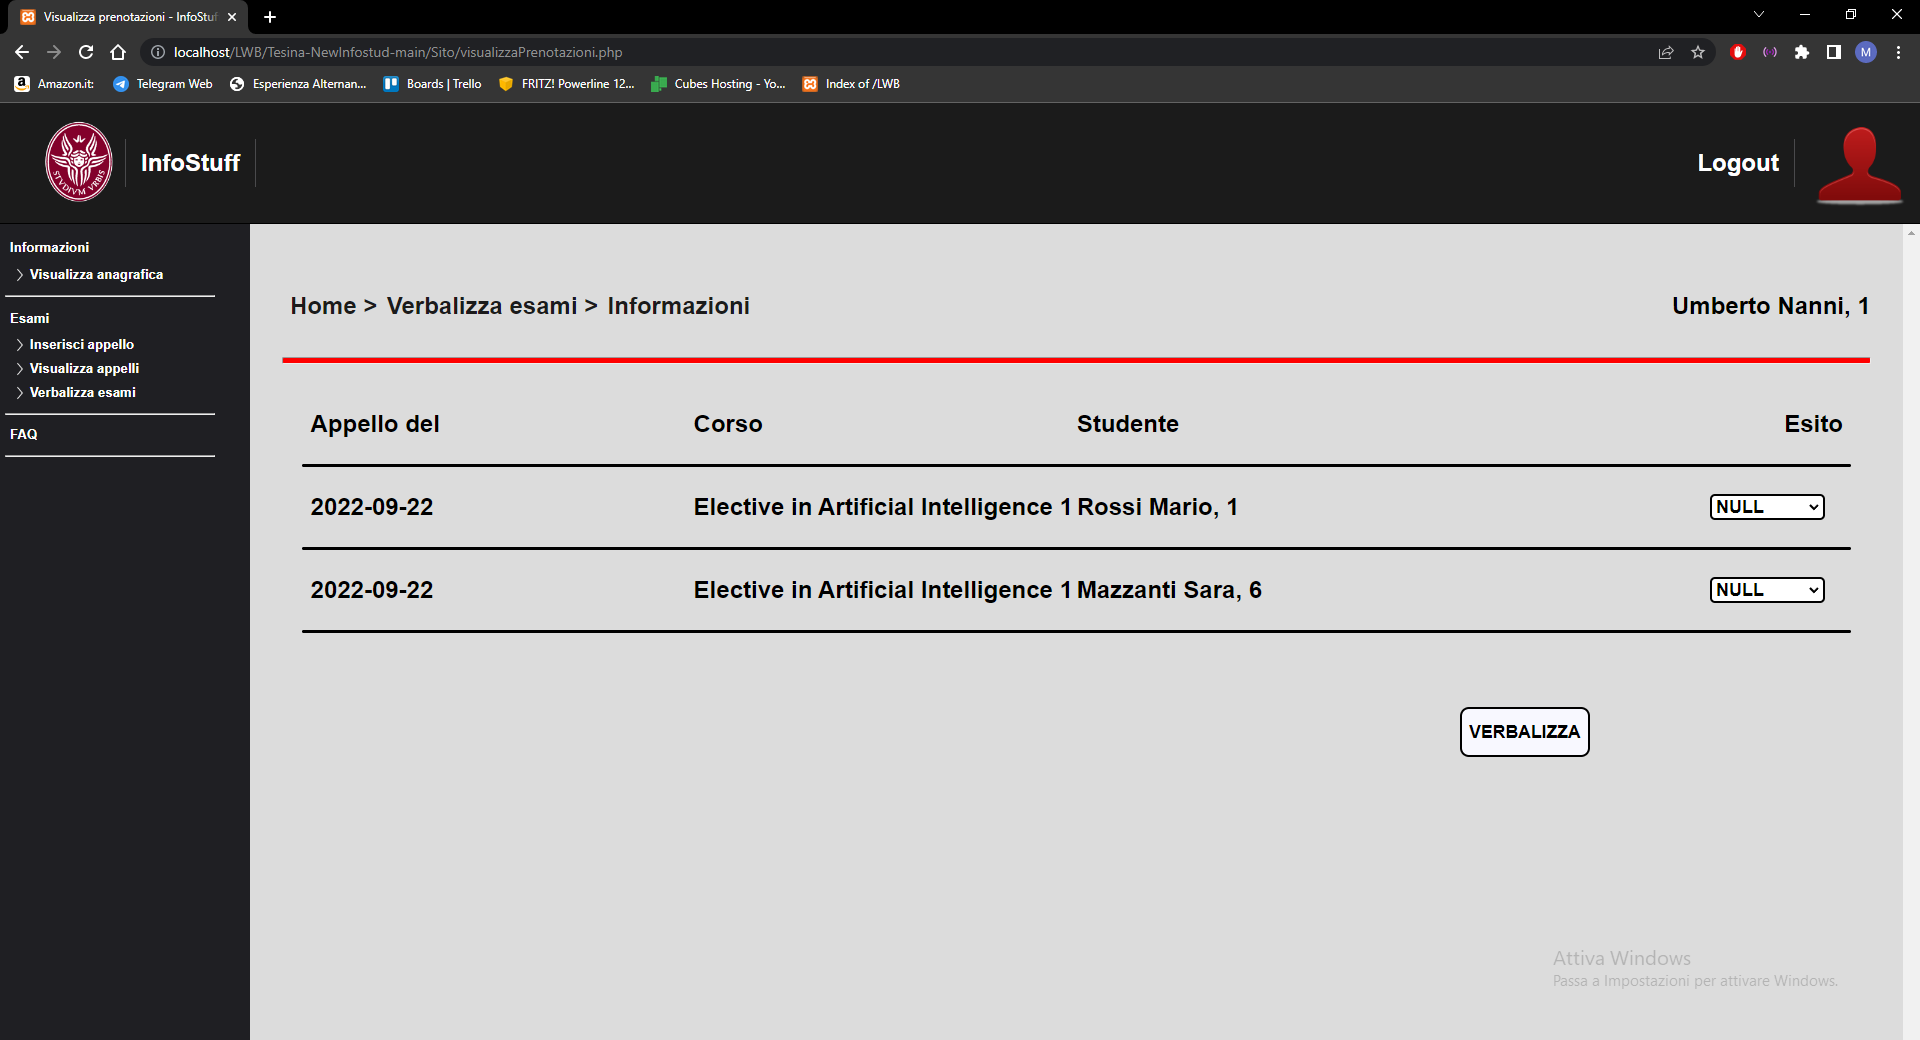
\includegraphics[scale=0.3]{figura2-27.png}
\caption{Pagina di verbalizzazione di un esame.}
\end{figure}

\medskip

\subsection{Accedere alle FAQ}

A partire da una qualsiasi pagina web relativa all'utenza, \textbf{qualora l'utente non fosse stato sospeso da un'utenza amministrativa}, è possibile cliccare sulla voce \emph{FAQ}, all'interno della barra laterale sita a sinistra della pagina stessa. L'utente - \textbf{se non sospeso} - verrà così reindirizzato ad una pagina web come quella in figura 2.28, nella quale verranno presentati a schermo tutti i corsi impartiti dal docente correntemente autenticato nella sessione corrente. La pressione di una delle apposite frecce laterali permetterà all'utente di accedere alla sezione delle FAQ relative al corso selezionato.

\begin{figure}
\centering
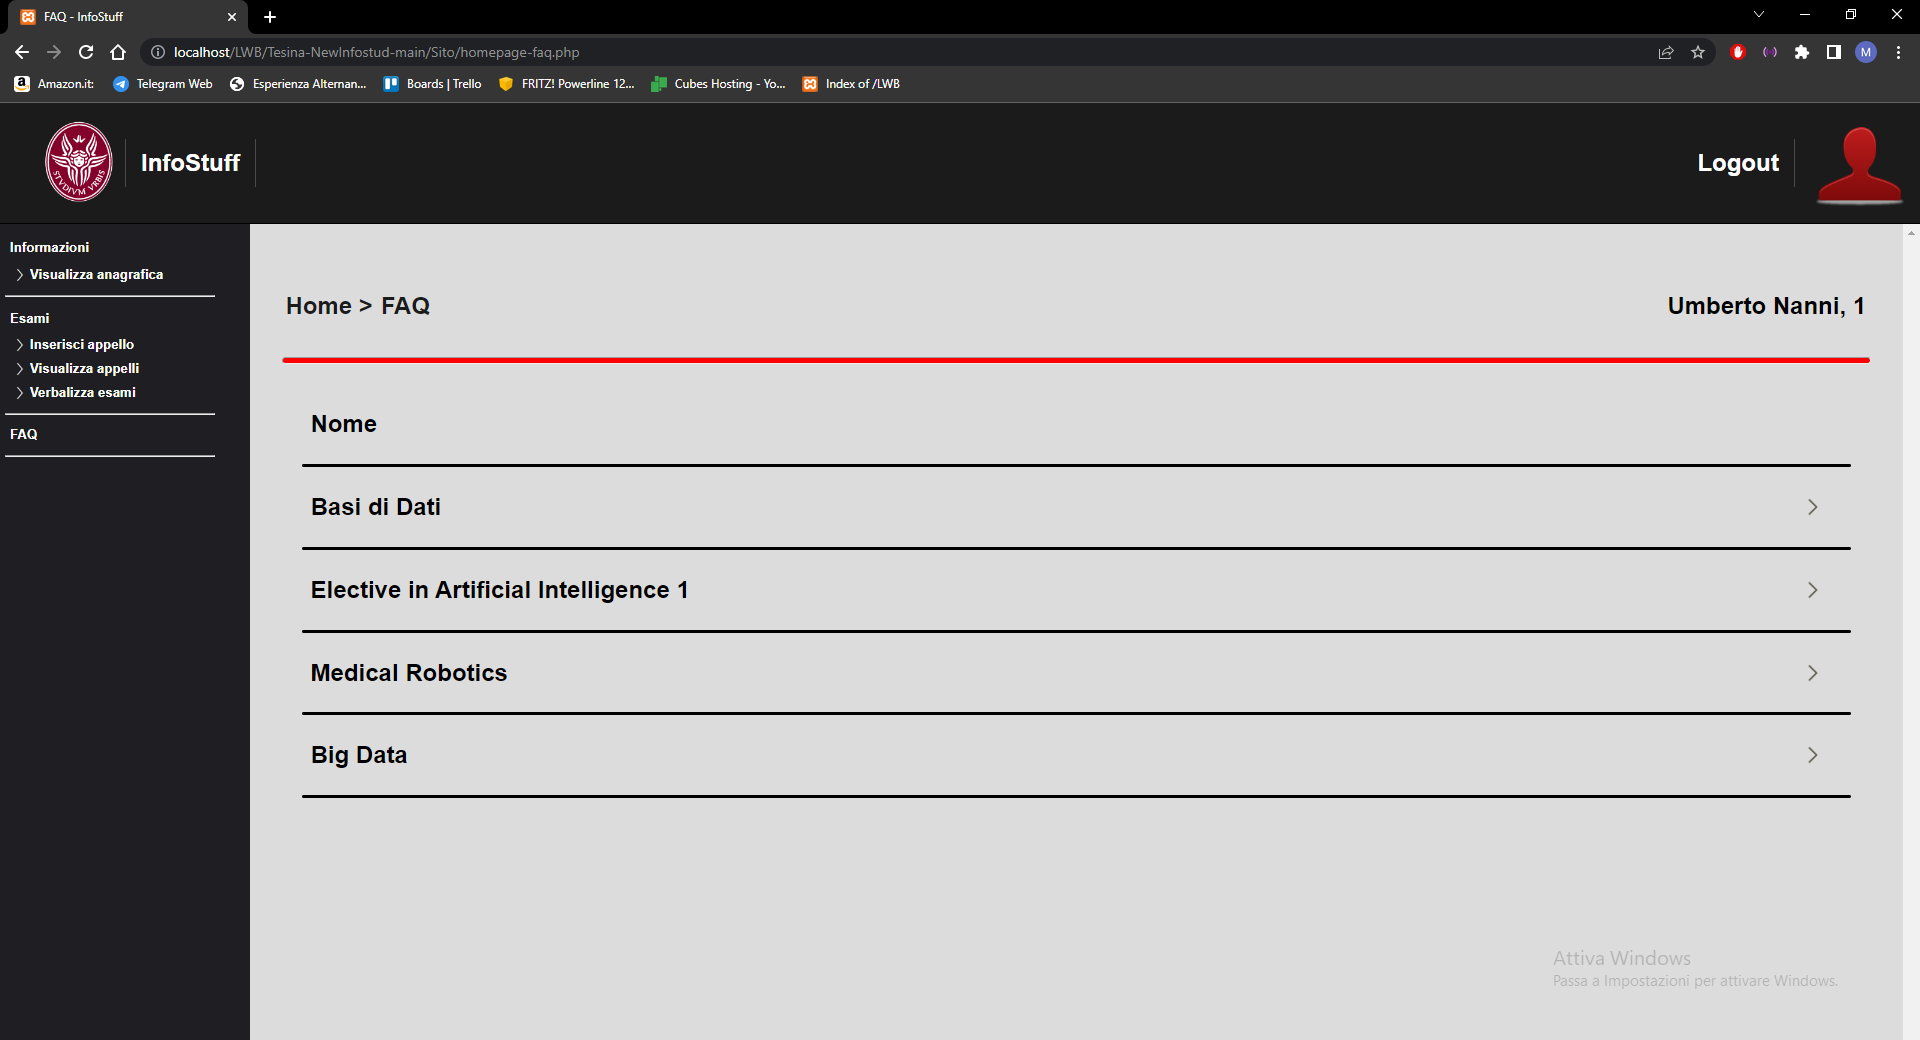
\includegraphics[scale=0.3]{figura2-28.png}
\caption{Visualizzazione dell'elenco dei corsi impartiti dal docente autenticato.}
\end{figure}

\medskip

\subsubsection{Interagire con le FAQ}

Premendo una freccia nella pagina di visualizzazione dei corsi impartiti dal docente autenticato nella sessione corrente, egli avrà accesso ad una sezione FAQ dedicata al corso selezionato. La pagina web presentata all'utente è simile a quella mostrata in figura 2.29. Vi è una suddivisione della pagina web in due macro-aree: la prima contenente le domande a cui è stata data risposta, visualizzate in ordine decrescente per utilità della domanda stessa; la seconda contenente invece le domande a cui ancora non è stata fornita alcuna risposta. 

\begin{figure}
\centering
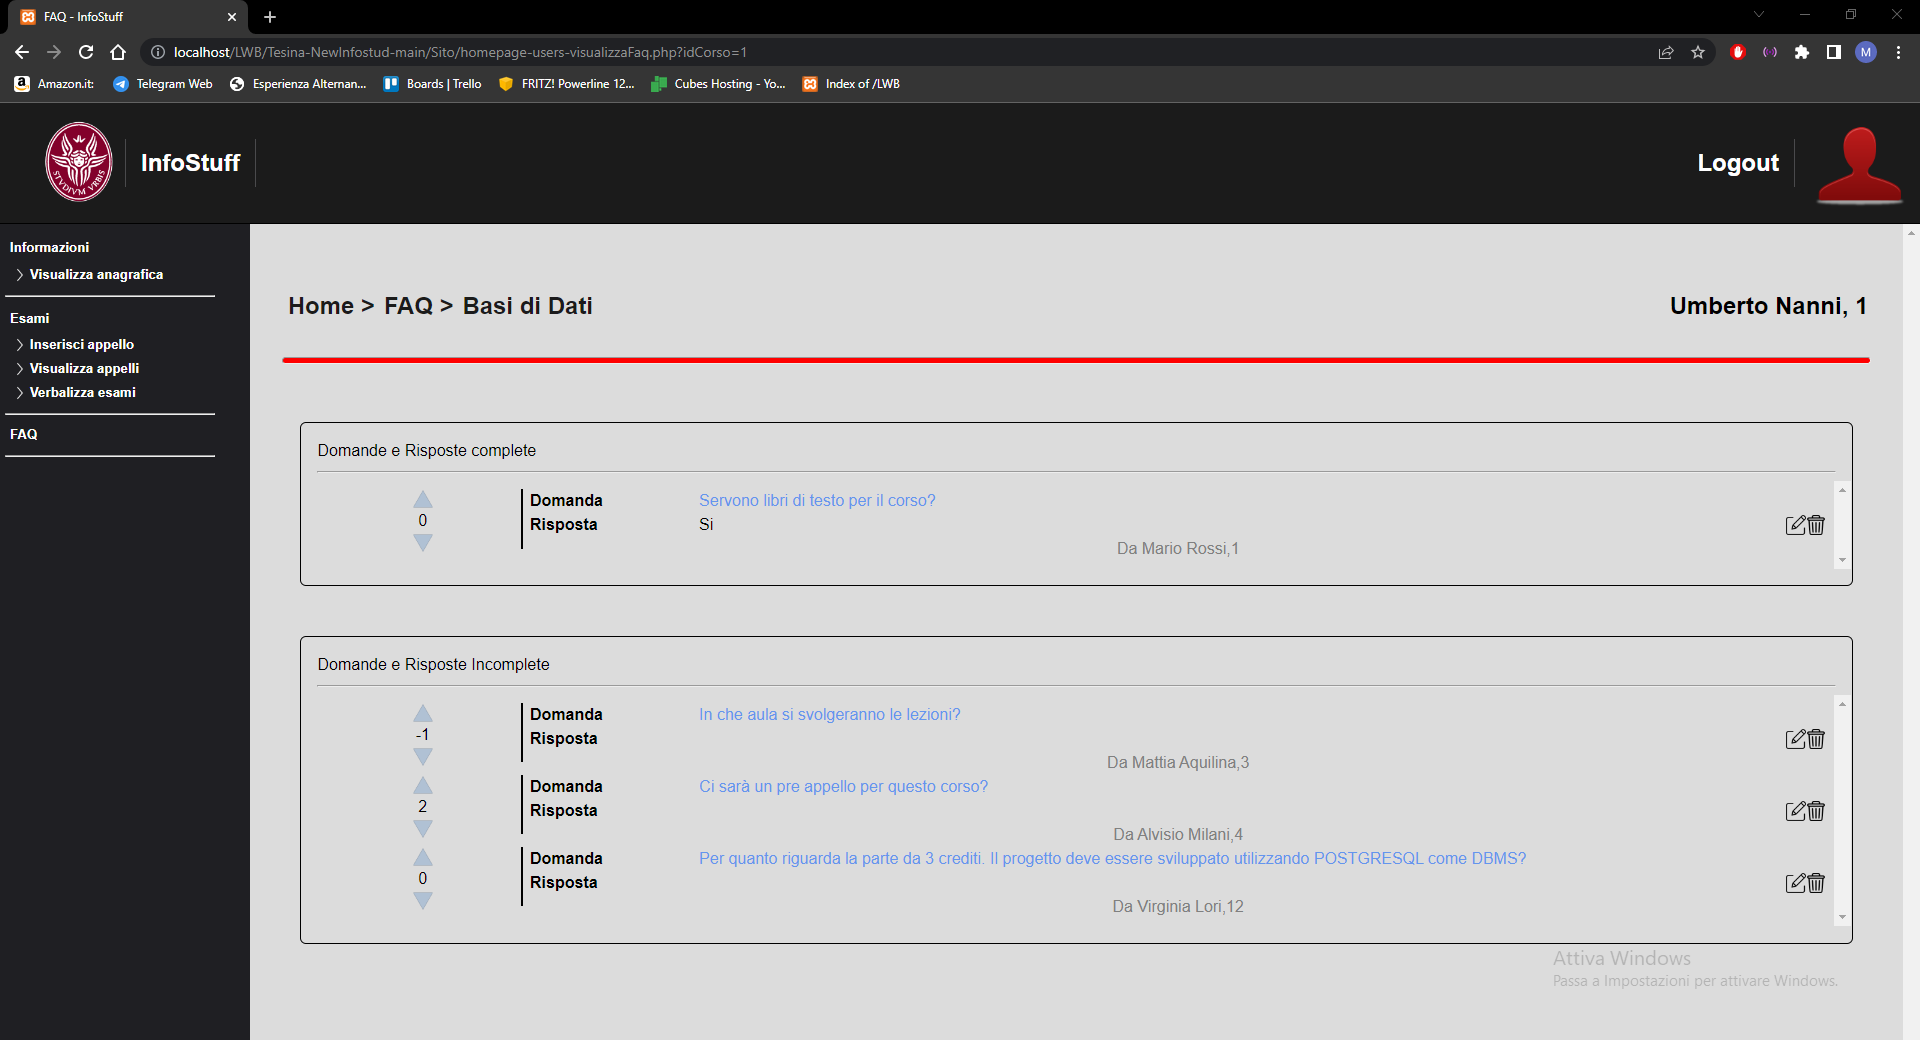
\includegraphics[scale=0.3]{figura2-29.png}
\caption{Sezione FAQ relativa ad un corso.}
\end{figure}

Nella prima area, il docente può modificare la propria risposta ad una o più domande, oppure può decidere di eliminare la domanda stessa. Nella seconda area, invece, il docente può inserire una risposta ad una domanda ancora priva di quest'ultima, oppure eliminarla; nel caso in cui il docente decidesse di rispondere ad una domanda presente nella seconda area, questa verrà immediatamente trasferita nella prima, in modo da poter essere visualizzata da tutti gli studenti aventi tale diritto.

\textbf{\underline{Attenzione}}: ricordiamo al lettore che un docente può accedere alla sezione delle FAQ dei propri corsi solo e soltanto se non è stato sospeso (\emph{soft ban}) da un'utenza amministrativa.

\medskip
\medskip

\section{Segretario}

\subsection{Visualizzare l'anagrafica}

Una volta effettuato il login, ad un'utenza di tipologia \emph{Segretario} verrà presentata una pagina web in cui saranno visualizzate le proprie informazioni di login, quali username e password; quest'ultima verrà visualizzata coperta da degli asterischi, che rappresentano la lunghezza della relativa password criptata secondo l'algoritmo di cifratura MD5. Come per ogni altra utenza nella piattaforma, anche un segretario può cambiare la propria password, premendo sull'apposita icona situata a fianco della password stessa (figura 2.30). 

\begin{figure}
\centering
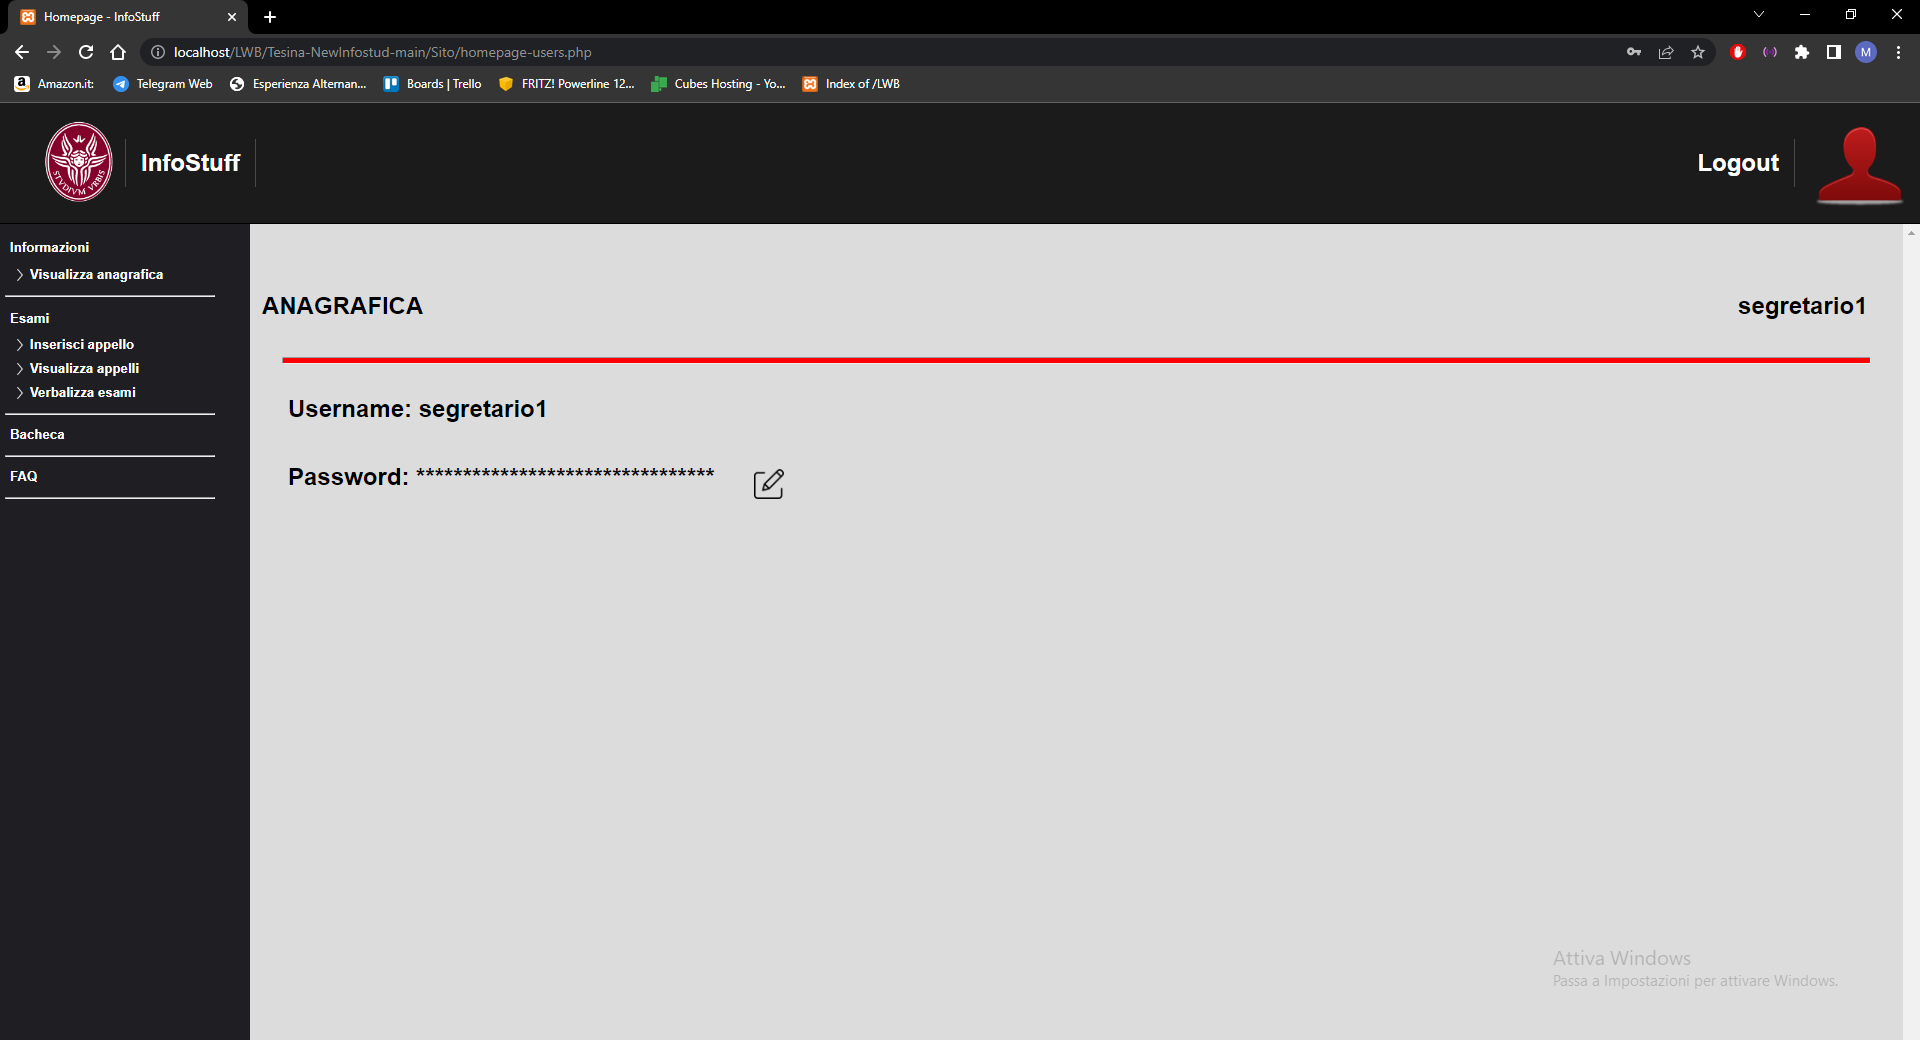
\includegraphics[scale=0.3]{figura2-30.png}
\caption{Homepage dell'utenza \emph{Segretario}.}
\end{figure}

In questa homepage, inoltre, viene presentata una sidebar con tutte le funzionalità relative alla segreteria, e che saranno descritte nel seguito di questo paragrafo. Si ricorda al lettore che, da qualsiasi pagina web del sito, è possibile tornare alla propria homepage di utenza cliccando sull'opportuna icona situata in alto a destra. Inoltre, da qualsiasi pagina web del sito, è possibile effettuare il logout: sarà sufficiente premere sull'apposito bottone sito anch'esso in alto a destra, a fianco dell'icona appena citata.

\medskip

\subsection{Visualizzare gli appelli}

A partire da una qualsiasi pagina web relativa all'utenza, è possibile cliccare sulla voce \emph{Visualizza appelli}, sotto la sezione \emph{Esami}, all'interno della barra laterale sita a sinistra della pagina stessa. L'utente verrà così reindirizzato ad una pagina web come quella in figura 2.31, nella quale verranno presentati a schermo tutti gli appelli di tutti i corsi registrati presso la piattaforma - inerenti, cioè, a qualsiasi corso di laurea registrato. In particolare, verranno visualizzati tutti gli appelli aventi data pari o successiva a quella corrente; la visualizzazione degli appelli è ordinata in base al seguente criterio: viene data la priorità all'ordinamento per nome del corso cui l'appello fa riferimento e, in seguito, gli appelli inerenti allo stesso corso vengono visualizzati in ordine cronologico.

\begin{figure}
\centering
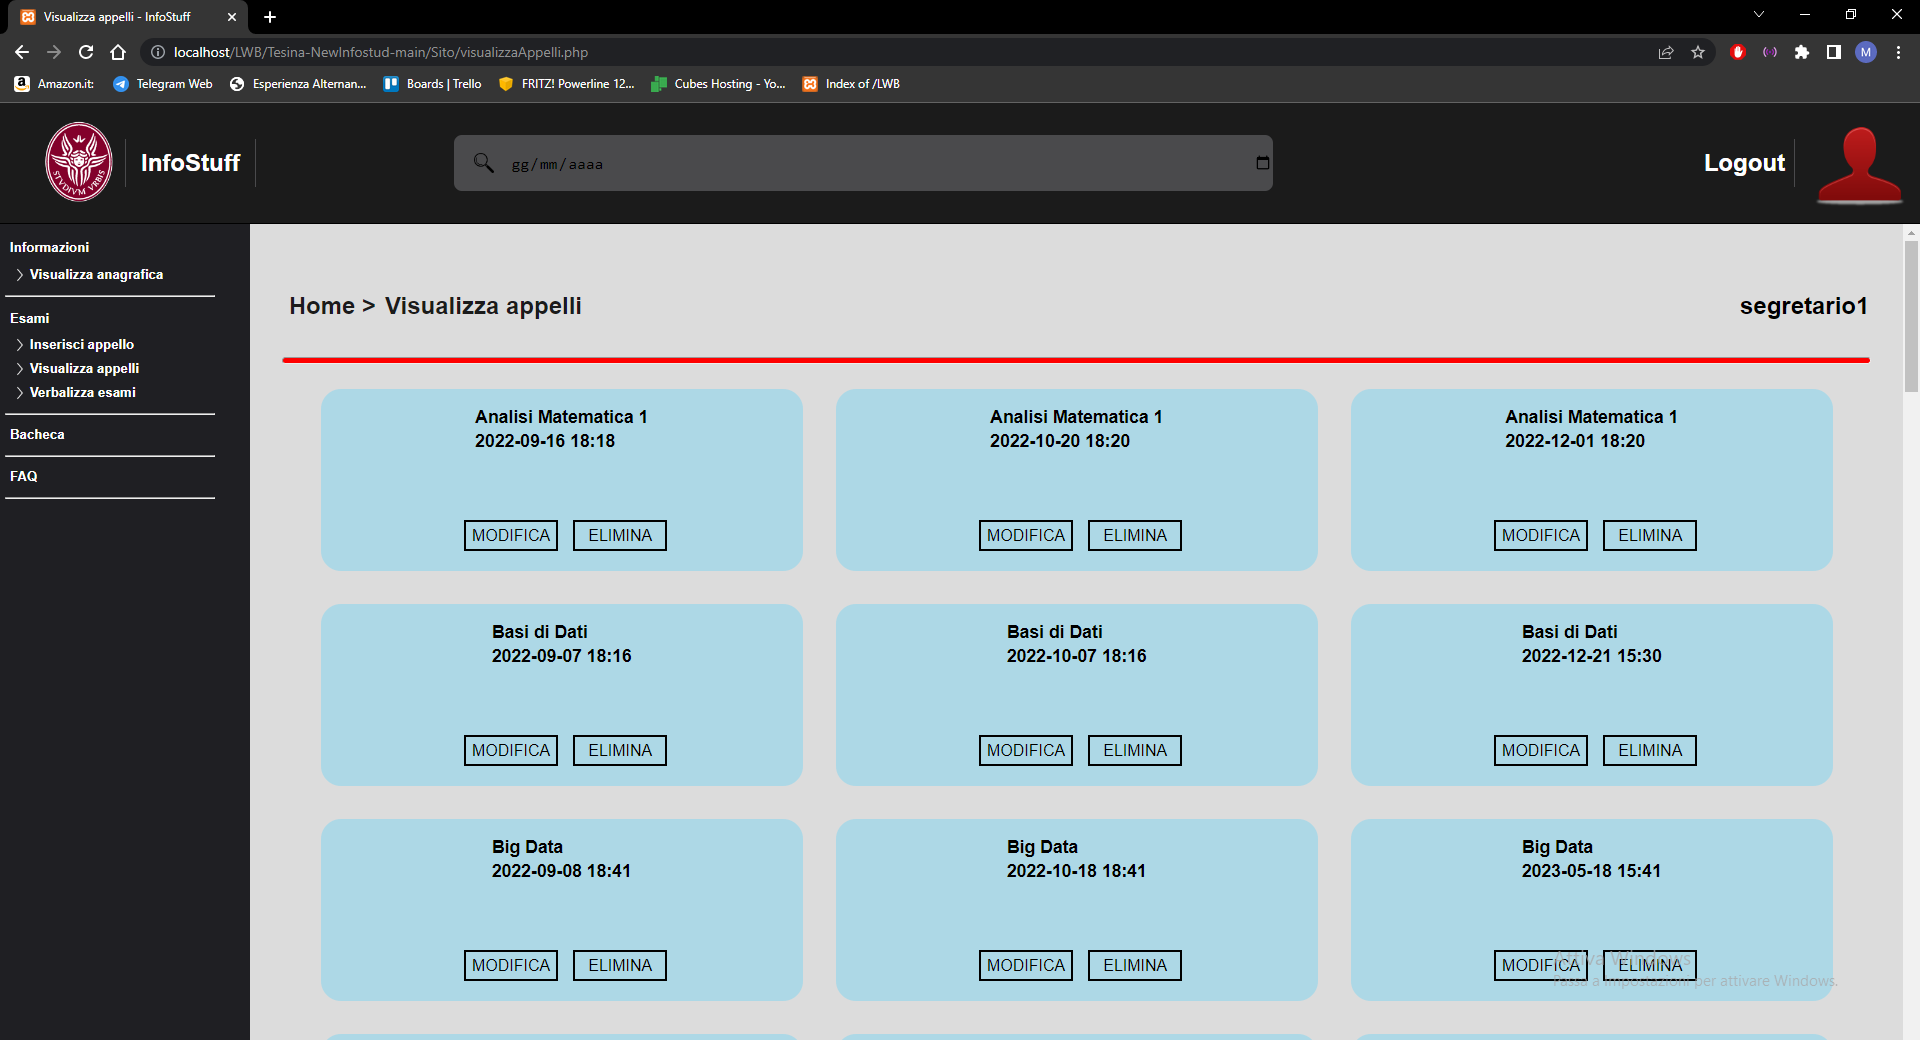
\includegraphics[scale=0.3]{figura2-31.png}
\caption{Visualizzazione di tutti gli appelli relativi a tutti i corsi di laurea registrati nella piattaforma.}
\end{figure}

Il segretario, a questo punto, dispone di tre scelte: può modificare un singolo appello, può eliminare un singolo appello, oppure può effettuare una ricerca di un appello mediante l'apposita barra di ricerca. La ricerca avviene tramite un meccanismo basato sulla data: in seguito alla ricerca, verranno visualizzati tutti gli appelli avente data pari o successiva a quella inserita.

\medskip

\subsubsection{Modificare un appello}

A partire dalla pagina di visualizzazione degli appelli, un segretario può decidere di modificare un singolo appello: sarà sufficiente cliccare sull'apposito bottone \emph{modifica}, che si trova in corrispondenza dell'appello stesso, come mostrato in figura 2.31. La pressione di questo bottone porterà l'utente in una nuova pagina web, contenente una form di modifica dell'appello: i campi della form, come mostrava la figura 2.23, sono già compilati con i dati dell'appello dal quale si proviene. L'utente sarà dunque libero di modificare i dati dell'appello a proprio piacimento; cliccando su \emph{invio}, l'appello verrà generalmente modificato. Tuttavia, in caso di corrispondenze con altri appelli, prima che la modifica venga effettuata, verrà mostrata all'utente una pagina web di segnalazione della corrispondenza avvenuta, come mostrato in figura 2.24.

In ogni caso, l'avvenuta modifica verrà segnalata da un opportuno avviso di successo; dualmente, in caso di errore, l'utente riceverà un'opportuna segnalazione.

\medskip

\subsubsection{Eliminare un appello}

A partire dalla pagina di visualizzazione degli appelli, un segretario può decidere di eliminare un singolo appello: sarà sufficiente cliccare sull'apposito bottone \emph{elimina}, che si trova in corrispondenza dell'appello stesso, come mostrato in figura 2.31. La pressione di questo pulsante scatenerà l'esecuzione di una funzione di eliminazione che, dopo una prima conferma da parte dell'utente, \emph{eliminerà} l'appello selezionato (per ulteriori approfondimenti sull'eliminazione, si faccia riferimento al capitolo 3).

L'avvenuta eliminazione verrà segnalata da un opportuno avviso di successo; dualmente, in caso di errore, l'utente riceverà un'opportuna segnalazione.

\medskip

\subsection{Inserire un appello}

A partire da una qualsiasi pagina web relativa all'utenza, è possibile cliccare sulla voce \emph{Inserisci appello}, sotto la sezione \emph{Esami}, all'interno della barra laterale sita a sinistra della pagina stessa. L'utente verrà così reindirizzato ad una pagina web come quella in figura 2.25, nella quale verrà presentata a schermo una form per l'inserimento di un nuovo appello. L'utente potrà dunque scegliere una qualsiasi data, purché successiva a quella corrente, un qualsiasi orario e uno dei corsi fra quelli registrati nella piattaforma; tutte queste informazioni sono obbligatorie. Premendo poi il pulsante \emph{invio}, le informazioni inserite andranno a costituire un nuovo appello, a meno di \textbf{collisioni}. L'utente potrà verificare l'avvenuto inserimento del nuovo appello mediante l'apposita funzionalità di visualizzazione degli appelli, trattata poc'anzi.

Inserendo un appello in prossimità di altri appelli relativi a corsi di uno stesso anno inerenti ad uno stesso corso di laurea, si avrà una \emph{corrispondenza}. In occorrenza di tale evento, prima che avvenga l'effettivo inserimento (o l'effettiva modifica!) dell'appello in questione, l'utente verrà reindirizzato verso una pagina web in cui viene segnalata la presenza di corrispondenze, e in cui vengono presentate le corrispondenze rilevate, al fine di dar modo al docente di prendere la sua decisione sull'effettivo inserimento (o sull'effettiva modifica) dell'appello stesso. Come già citato, un'esemplificazione di una tale pagina web è riportata in figura 2.24. Rispondendo \emph{sì} alla domanda ''\emph{Sono state rilevate corrispondenze. Inserire comunque l'appello?}'', l'inserimento avverrà senza altri indugi; altrimenti, rispondendo \emph{no}, l'utente verrà reindirizzato alla pagina di inserimento (o di modifica) dell'appello, nella quale troverà la form già compilata con i dati precedentemente inseriti.

\medskip

\subsection{Verbalizzare gli esami}

A partire da una qualsiasi pagina web relativa all'utenza, è possibile cliccare sulla voce \emph{Verbalizza esami}, sotto la sezione \emph{Esami}, all'interno della barra laterale sita a sinistra della pagina stessa. L'utente verrà così reindirizzato ad una pagina web come quella in figura 2.32, nella quale verranno presentati a schermo tutti gli appelli di tutti i corsi registrati presso la piattaforma - inerenti, cioè, a tutti i corsi di laurea presenti. In particolare, verranno visualizzati tutti gli appelli aventi data pari o successiva a quella corrente; la visualizzazione degli appelli è ordinata in base al seguente criterio: viene data la priorità all'ordinamento per nome del corso cui l'appello fa riferimento e, in seguito, gli appelli inerenti allo stesso corso vengono visualizzati in ordine cronologico.

\begin{figure}
\centering
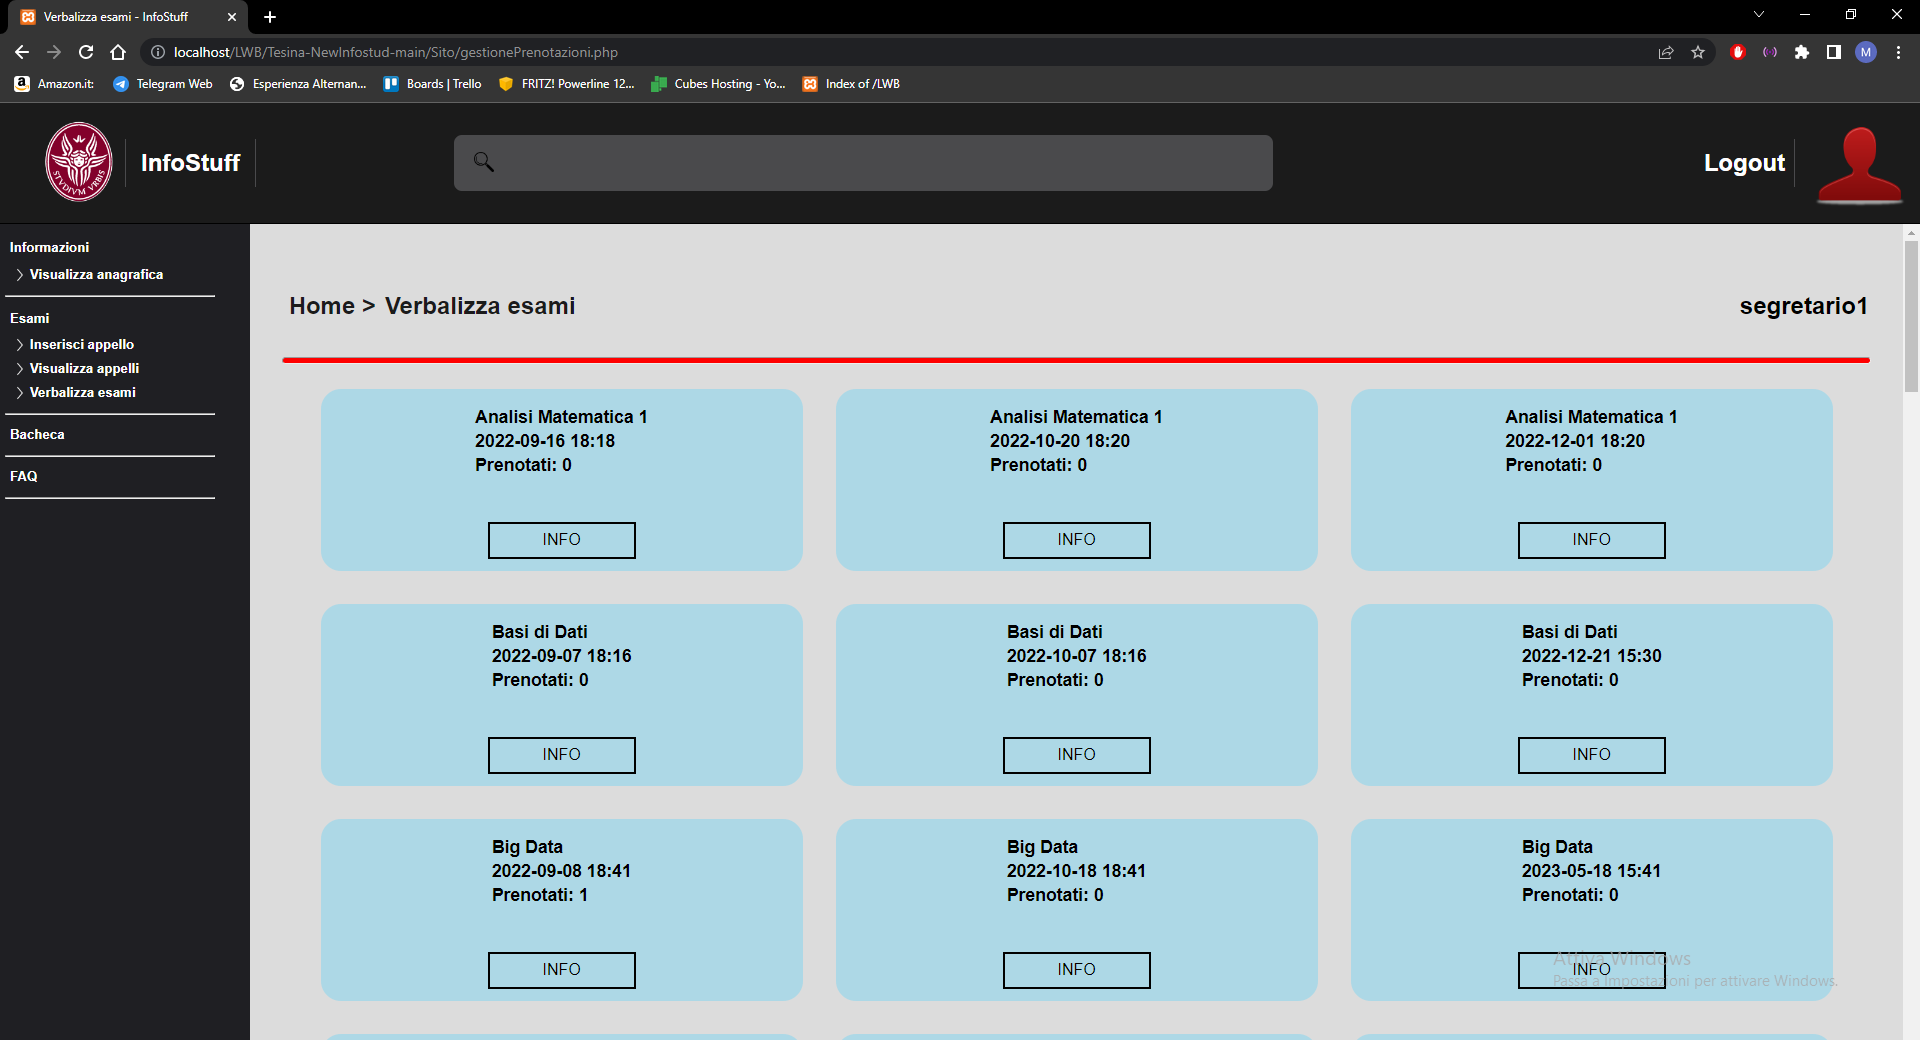
\includegraphics[scale=0.3]{figura2-32.png}
\caption{Visualizzazione di tutti gli appelli relativi a tutti i corsi registrati presso la piattaforma.}
\end{figure}

A differenza della semplice visualizzazione, questa volta gli appelli vengono presentati con un'informazione aggiuntiva: il numero di studenti prenotati ai singoli appelli. Inoltre, come mostrato in figura 2.32, i singoli appelli dispongono di un pulsante \emph{info}, premendo il quale l'utente potrà accedere alla pagina web per l'effettiva verbalizzazione, mostrata in figura 2.27. Tale pagina avrà lo scopo di visualizzare una lista di tutti gli studenti iscritti all'appello selezionato; il segretario potrà inserire la relativa valutazione nell'apposito campo \emph{esito} e, premendo sul pulsante \emph{verbalizza}, verrà effettuata la verbalizzazione di tutti gli esami aventi esito diverso da NULL. Come discusso nel capitolo 1 \hyperref[sec:specifiche]{\textcolor{gray}{[$\uparrow$]}}, l'esito di un esame verbalizzato può essere un numero compreso fra 18/30 e 30/30 con lode (il valore di un 30/30 con lode è pari a 31), oppure può essere una lettera, R o B; la lettera R indica il ritiro da parte dello studente dallo svolgimento dell'esame, mentre la lettera B indica una bocciatura, ossia la terminazione dell'esame svolto con esito negativo.

\medskip

\subsection{Accedere alle bacheche}

La fruizione delle bacheche è un'importante ed innovativa funzionalità offerta dalla piattaforma e si compone di diversi strumenti messi a disposizione agli studenti, \textbf{purché non siano stati sospesi da un'utenza amministrativa}. Qui, il ruolo svolto dalla segreteria è un ruolo di \emph{moderazione}: un segretario, cioè, non può prendere parte in modo attivo alle votazioni di post e commenti, ma è in grado di creare post di avviso, così come di commentare sotto ogni tipologia di post, in modo da far percepire alla community studentesca una presenza autorevole atta a garantire il giusto grado di ordine nelle varie bacheche. Qualora gli studenti non dovessero rispettare le più banali norme di comportamento, un segretario può scegliere di modificare o di eliminare il contenuto di un post o di un commento.

A partire da una qualsiasi pagina web relativa all'utenza, è possibile cliccare sulla voce \emph{Bacheca}, all'interno della barra laterale sita a sinistra della pagina stessa. L'utente, \textbf{a patto di non essere stato sospeso da un'utenza amministrativa}, verrà reindirizzato ad una pagina web come quella in figura 2.33, nella quale vengono elencati tutti i corsi appartenenti a tutti i corsi di laurea registrati all'interno della piattaforma.

\begin{figure}
\centering
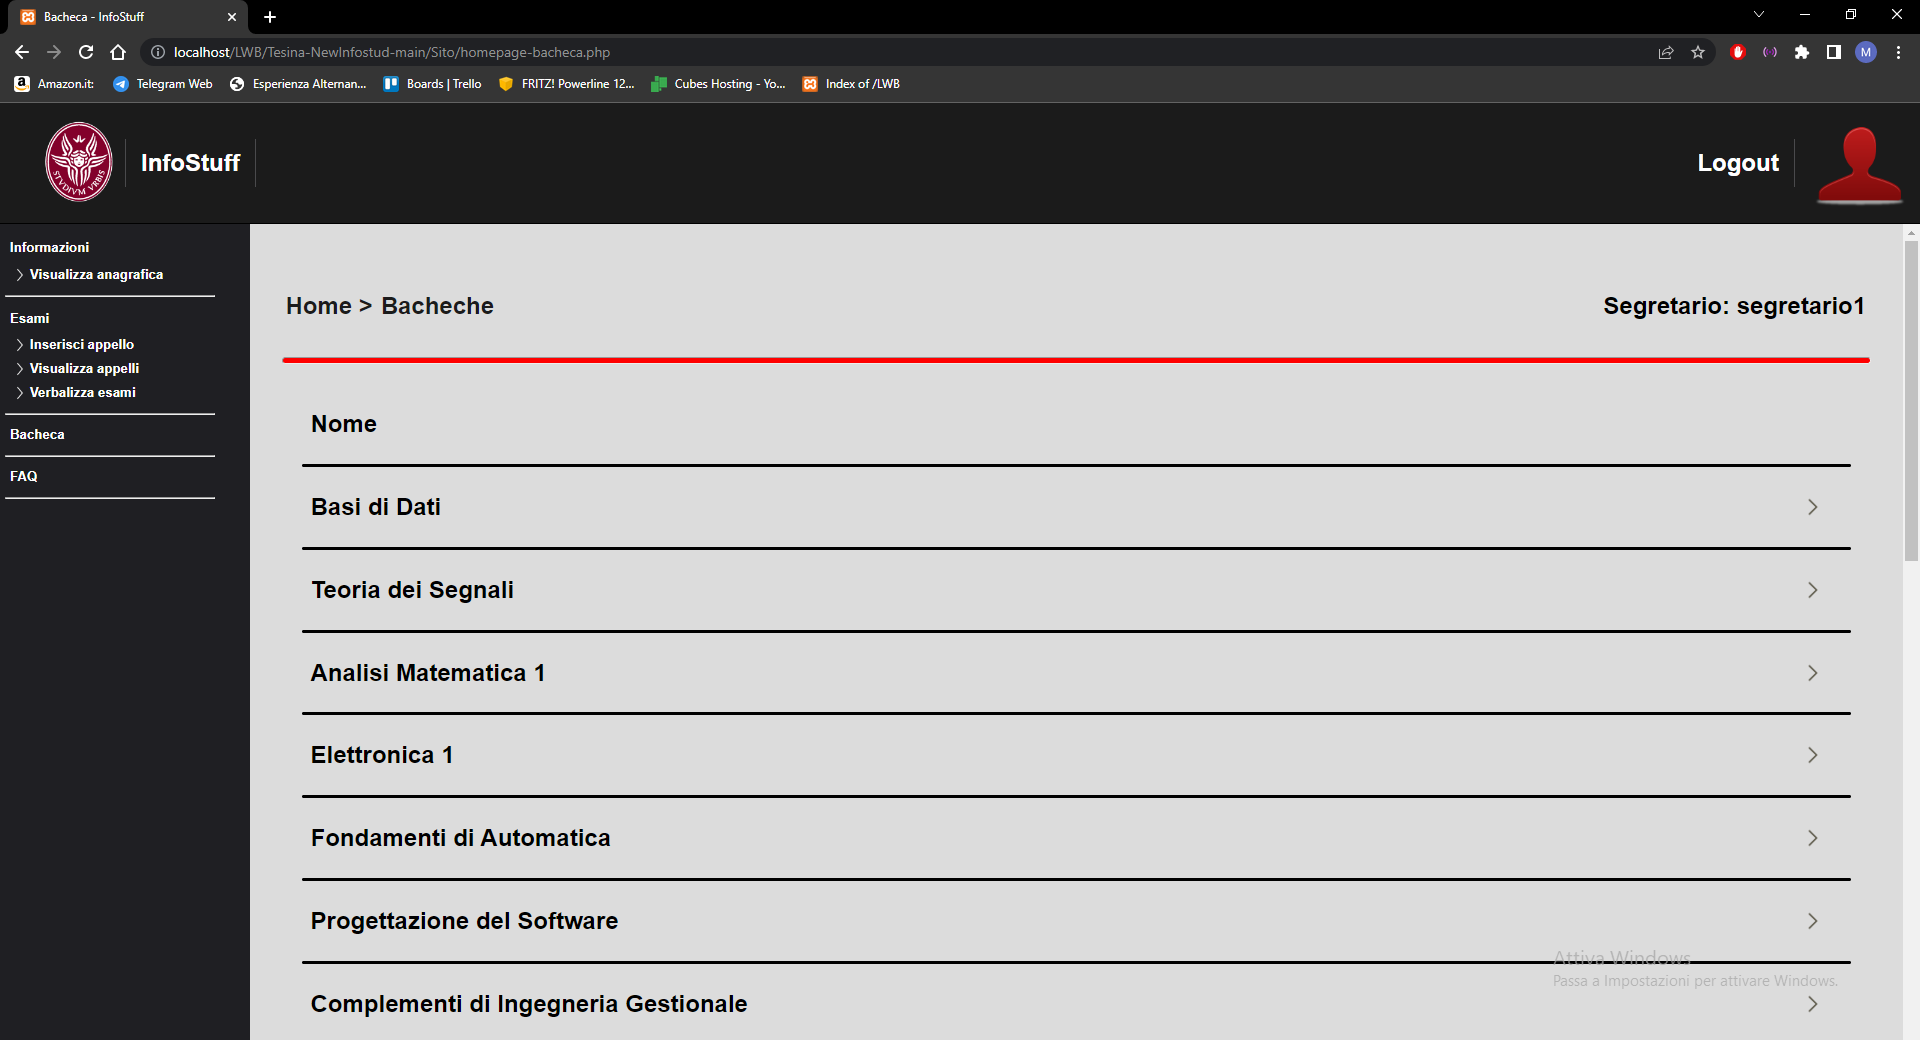
\includegraphics[scale=0.3]{figura2-33.png}
\caption{Lista dei corsi relativi a tutti i corsi di laurea memorizzati nella piattaforma.}
\end{figure}

In questa pagina web, ciascuna voce rappresenta la bacheca dei singoli corsi. Interagendo con una di queste voci, l'utente viene reindirizzato ad una pagina web simile a quella mostrata in figura 2.16. La pagina in questione rappresenta una singola bacheca associata ad un determinato corso. Essa consiste di un menù di navigazione, posto nella parte superiore del corpo della bacheca, che consente all'utente di attraversare le diverse pagine della bacheca stessa (\emph{facciamo notare che il numero di post che possono essere visualizzati per pagina è pari a 5}). Sempre nella parte superiore, allo stesso livello del menù di navigazione, è presente un bottone \emph{crea post}, la cui pressione scatena un evento di creazione o di eliminazione di una form, posta al di sopra dell'elenco dei post (figura 2.17). Tramite questa form è possibile pubblicare un nuovo al post all'interno della bacheca.

Nel blocco centrale della pagina web, troviamo l'elenco vero e proprio dei post relativi alla singola bacheca selezionata. In cima alla lista dei post è presente una barra orizzontale, che ci permette di applicare alcuni filtri di visualizzazione dei post sottostanti, fra i quali possiamo citare l'ordinamento sull'utilità dei post, sul numero di risposte ai singoli post e sulla data di pubblicazione dei singoli post. Inoltre, in ogni bacheca vengono sempre posti in sovraimpressione i due post che hanno ricevuto più voti utilità, e vengono separati dall'elenco tramite un separatore a forma di barra orizzontale celeste. Interagendo con una voce dell'elenco visualizzato, si raggiunge una pagina che visualizza il post scelto, la cui descrizione è contenuta nella sezione successiva.

\medskip

\subsubsection{Interagire con i post}

L'interazione con il post avviene in un'apposita pagina di visualizzazione del contenuto di quest'ultimo. Analizzando la schermata dall'alto (cfr. figura 2.18), troviamo innanzitutto l'intestazione del post, che si compone di una coppia di frecce, utilizzate per votare l'utilità del post stesso, e da un blocco contente autore, data di pubblicazione e contenuto di quest'ultimo. Qualora l'utenza correntemente autenticata fosse anche l'autore del post in visualizzazione, nell'angolo in alto a destra verrebbero visualizzate due icone, che permettono rispettivamente di eliminare il post e di modificarne il contenuto.

A seguire, verranno visualizzati in colonna tutti i commenti pubblicati in risposta al post, fino ad un massimo di cinque per pagina. Qualora il numero di commenti superasse questo limite, è sempre possibile interagire con la barra di navigazione contenuta tra il post e la lista dei commenti, per attraversare le diverse pagine. 

Ricordiamo che un segretario non può prendere parte in modo attivo alle votazioni di post e commenti, ma è in grado di creare post di avviso, così come di commentare sotto ogni tipologia di post, in modo da far percepire alla community studentesca una presenza autorevole atta a garantire il giusto grado di ordine nelle varie bacheche. Qualora gli studenti non dovessero rispettare le più banali norme di comportamento, un segretario può scegliere di modificare o di eliminare il contenuto di un post o di un commento.

Infine, ai piedi della pagina, troviamo una sezione che permette all'utente di pubblicare un commento relativo al post correntemente visualizzato nella pagina web.

\medskip

\textbf{\underline{Attenzione}}: ricordiamo al lettore che un segretario può accedere alla sezione delle bacheche dei propri corsi solo e soltanto se non è stato sospeso (\emph{soft ban}) da un'utenza amministrativa.

\medskip

\subsection{Accedere alle FAQ}

Il sistema delle FAQ permette agli studenti di interagire con i docenti proponendo delle domande in appositi box, o di votare quelle già presenti; saranno poi i docenti a scegliere le domande alle quali rispondere e le domande che possono essere eventualmente eliminate. Qui, il ruolo svolto dalla segreteria è un ruolo di \emph{moderazione}: un segretario, cioè, non può prendere parte in modo attivo alle votazioni delle domande poste, ma è in grado di inserire nuove domande con annesse risposte, in modo da far percepire alla community una presenza autorevole atta a garantire il giusto grado di ordine nelle varie sezioni FAQ. Qualora gli studenti e/o i docenti non dovessero rispettare le più banali norme di comportamento, un segretario può scegliere di modificare o di eliminare il contenuto di una domanda o di una risposta.

A partire da una qualsiasi pagina web relativa all'utenza, è possibile cliccare sulla voce \emph{FAQ}, all'interno della barra laterale sita a sinistra della pagina stessa. L'utente, \textbf{a patto di non essere stato sospeso da un'utenza amministrativa}, alla pressione di tale pulsante verrà reindirizzato ad una pagina web come quella in figura 2.34, nella quale verrà presentata una lista dei corsi relativi a tutti i corsi di laurea registrati presso la piattaforma; da qui, l'utente può scegliere un corso e, interagendo con l'apposito pulsante, può raggiungere la pagina delle FAQ specifica per il corso selezionato.

\begin{figure}
\centering
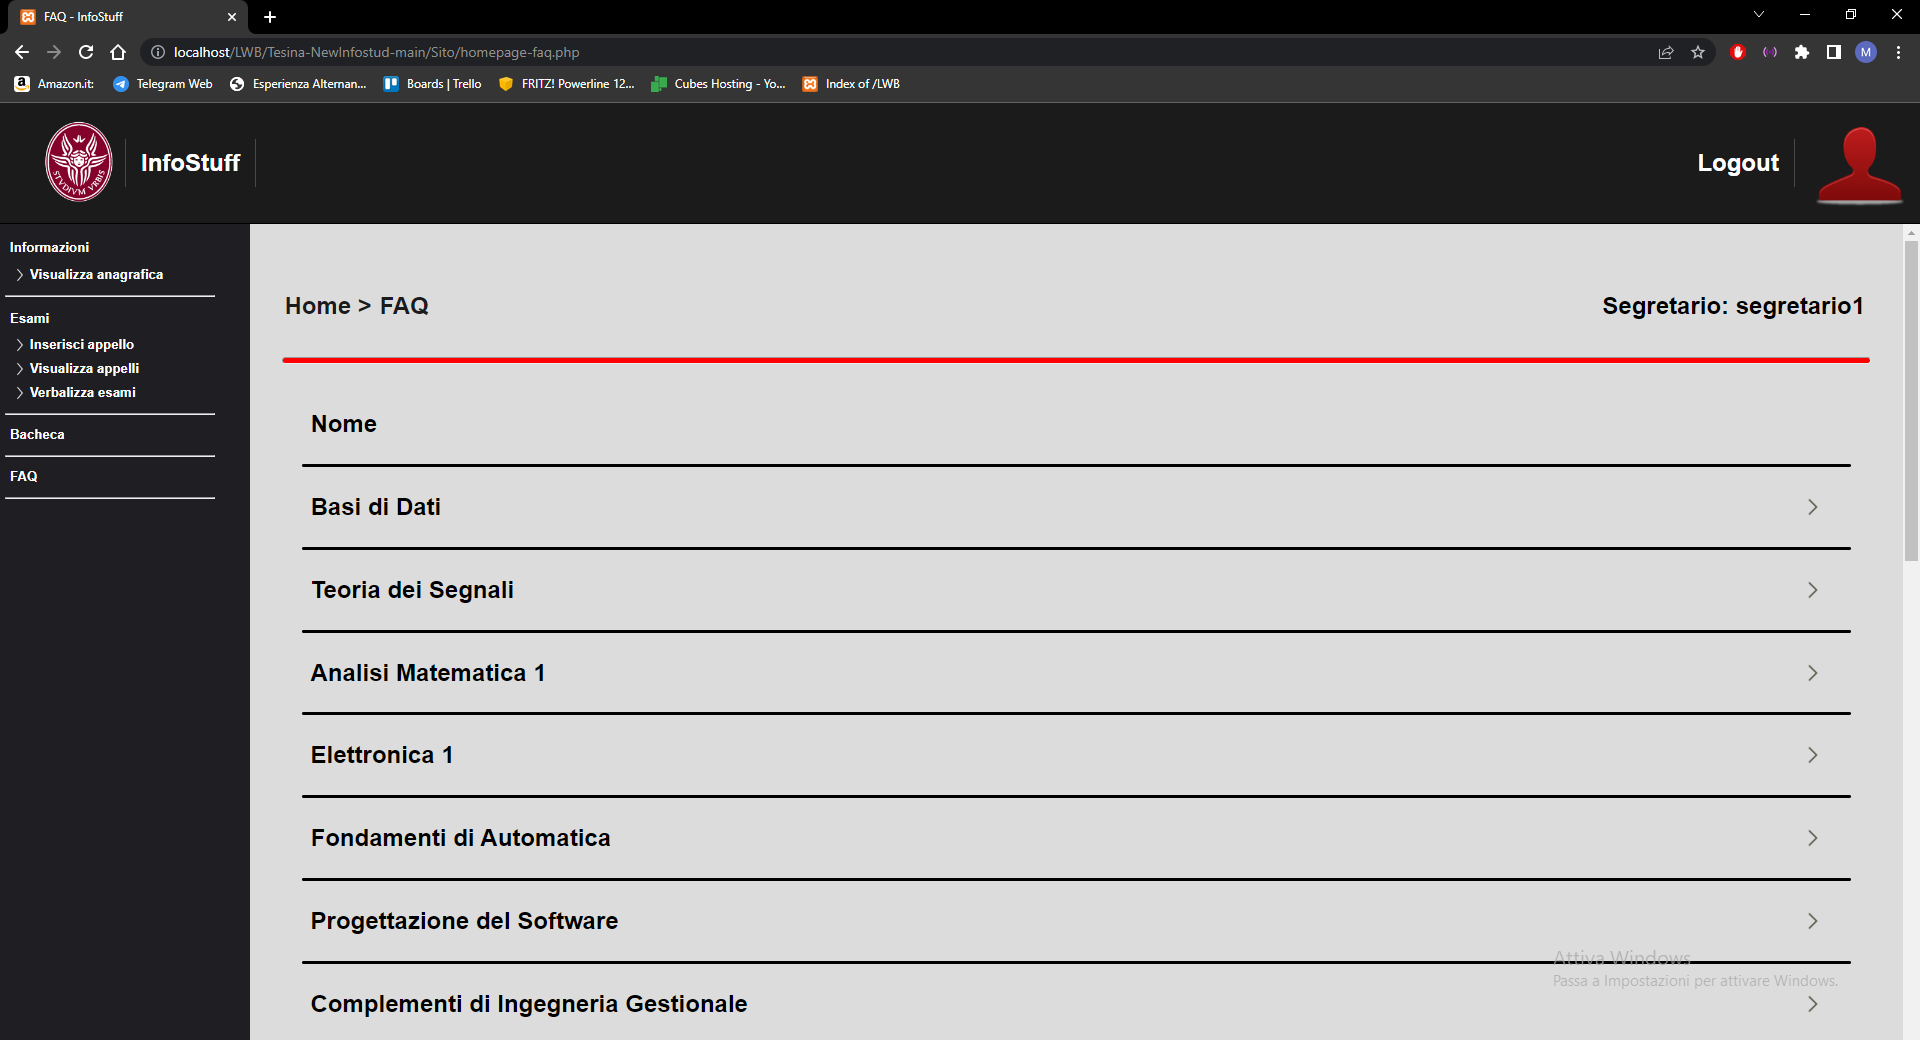
\includegraphics[scale=0.3]{figura2-34.png}
\caption{Lista dei corsi relativi a tutti i corsi di laurea memorizzati nella piattaforma.}
\end{figure}

La pagina che si presenterà al segretario, mostrata in figura 2.20, è divisa in tre aree. In cima troviamo un box che rappresenta il contenitore di tutte quelle domande che hanno ricevuto una risposta. Il secondo blocco rappresenta invece il container delle domande ancora incomplete, ossia delle domande alle quali nessuno ha ancora pubblicato una risposta. Per una qualsiasi domanda, è possibile interagire con la coppia di frecce poste alla sinistra del testo, per esprimere un voto di utilità riguardante il contenuto della FAQ proposta. In fondo alla pagina, infine, troviamo una form che consente all'utente di contribuire alla FAQ, permettendogli di pubblicare una nuova domanda. 

\medskip

\textbf{\underline{Attenzione}}: ricordiamo al lettore che un segretario può accedere alla sezione delle FAQ dei propri corsi solo e soltanto se non è stato sospeso (\emph{soft ban}) da un'utenza amministrativa.

\medskip
\medskip

\section{Amministratore}

\subsection{Visualizzare l'anagrafica}

Una volta effettuato il login, ad un'utenza di tipologia \emph{Amministratore} verrà presentata una pagina web in cui saranno visualizzate le proprie informazioni di login, quali username e password; quest'ultima verrà visualizzata coperta da degli asterischi, che rappresentano la lunghezza della relativa password criptata secondo l'algoritmo di cifratura MD5. Come per ogni altra utenza nella piattaforma, anche un amministratore può cambiare la propria password, premendo sull'apposita icona situata a fianco della password stessa (figura 2.35). 

\begin{figure}
\centering
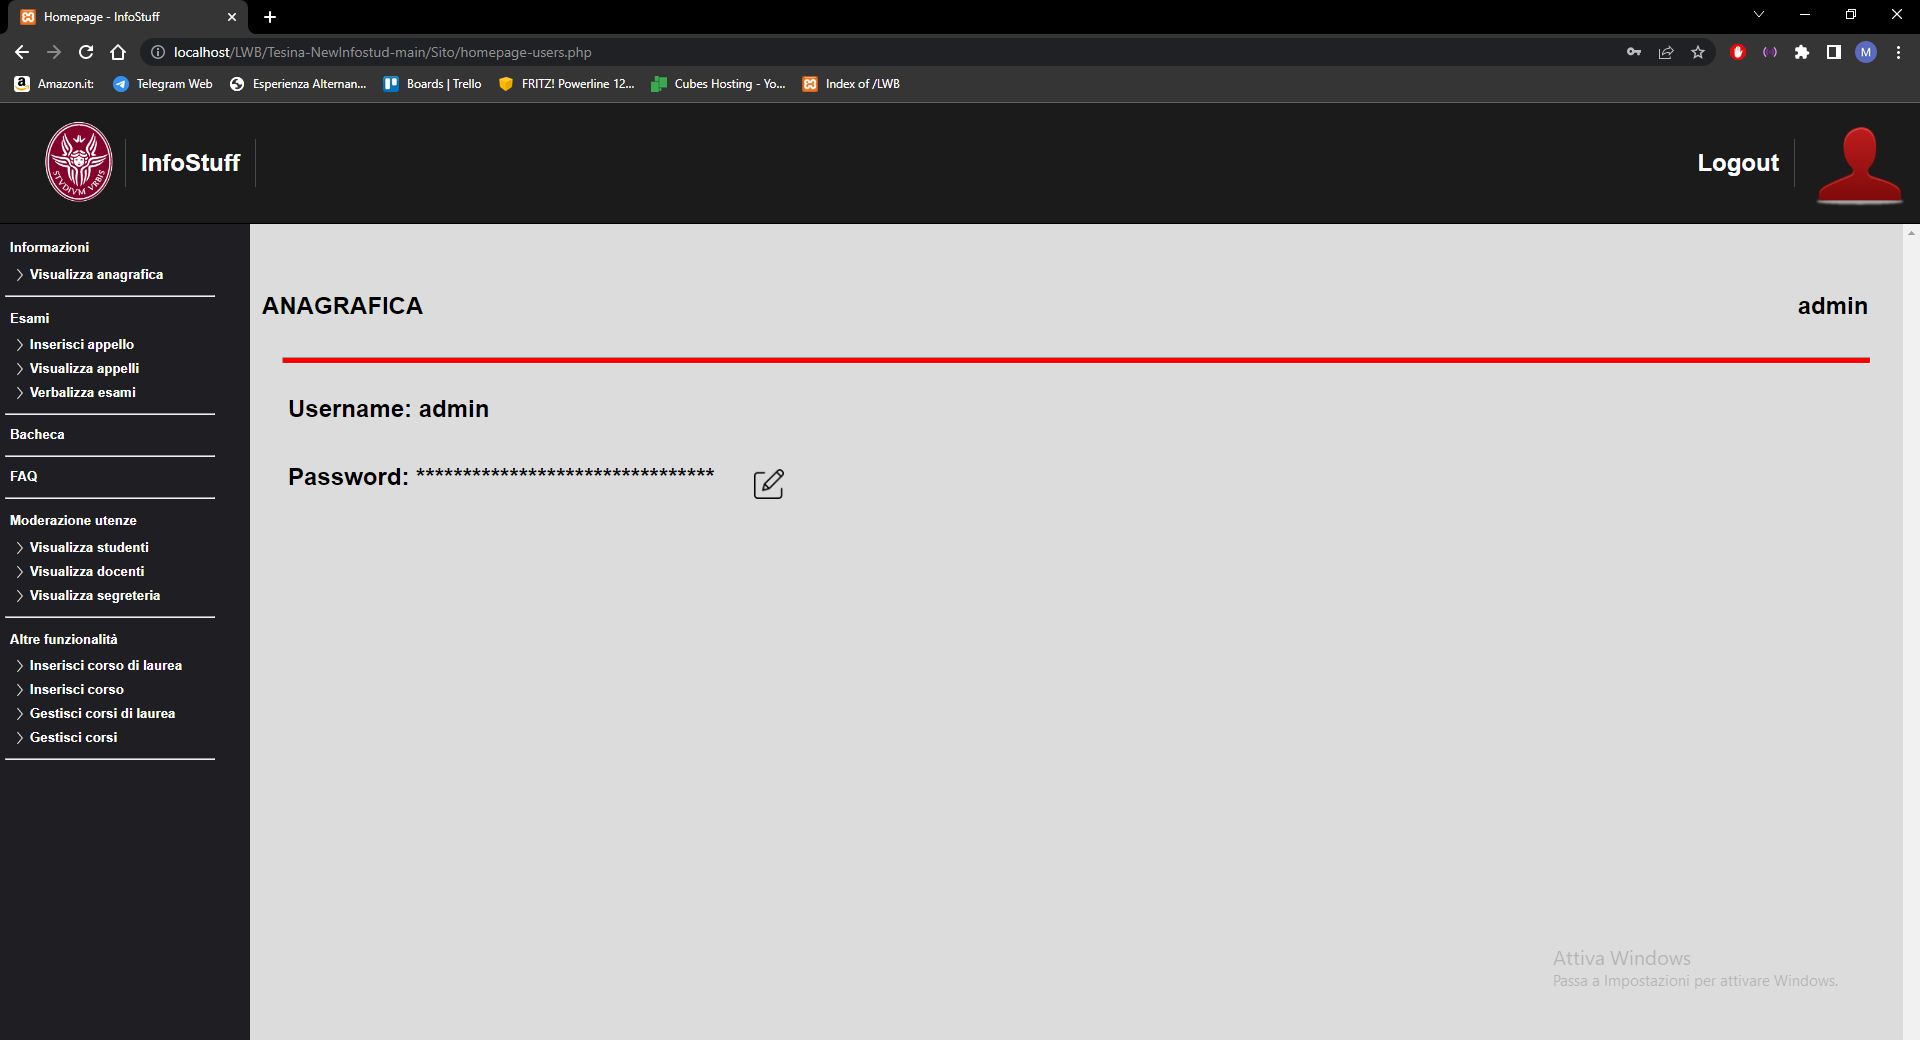
\includegraphics[scale=0.3]{figura2-35.png}
\caption{Homepage dell'utenza \emph{Amministratore}.}
\end{figure}

In questa homepage, inoltre, viene presentata una sidebar con tutte le funzionalità relative all'amministrazione, e che saranno descritte nel seguito di questo paragrafo. Si ricorda al lettore che, da qualsiasi pagina web del sito, è possibile tornare alla propria homepage di utenza cliccando sull'opportuna icona situata in alto a destra. Inoltre, da qualsiasi pagina web del sito, è possibile effettuare il logout: sarà sufficiente premere sull'apposito bottone sito anch'esso in alto a destra, a fianco dell'icona appena citata.

\medskip

\subsection{Visualizzare gli appelli}

A partire da una qualsiasi pagina web relativa all'utenza, è possibile cliccare sulla voce \emph{Visualizza appelli}, sotto la sezione \emph{Esami}, all'interno della barra laterale sita a sinistra della pagina stessa. L'utente verrà così reindirizzato ad una pagina web come quella in figura 2.31, nella quale verranno presentati a schermo tutti gli appelli di tutti i corsi registrati presso la piattaforma - inerenti, cioè, a qualsiasi corso di laurea registrato. In particolare, verranno visualizzati tutti gli appelli aventi data pari o successiva a quella corrente; la visualizzazione degli appelli è ordinata in base al seguente criterio: viene data la priorità all'ordinamento per nome del corso cui l'appello fa riferimento e, in seguito, gli appelli inerenti allo stesso corso vengono visualizzati in ordine cronologico.

L'amministratore, a questo punto, dispone di tre scelte: può modificare un singolo appello, può eliminare un singolo appello, oppure può effettuare una ricerca di un appello mediante l'apposita barra di ricerca. La ricerca avviene tramite un meccanismo basato sulla data: in seguito alla ricerca, verranno visualizzati tutti gli appelli avente data pari o successiva a quella inserita.

\medskip

\subsubsection{Modificare un appello}

A partire dalla pagina di visualizzazione degli appelli, un amministratore può decidere di modificare un singolo appello: sarà sufficiente cliccare sull'apposito bottone \emph{modifica}, che si trova in corrispondenza dell'appello stesso, come mostrato in figura 2.31. La pressione di questo bottone porterà l'utente in una nuova pagina web, contenente una form di modifica dell'appello: i campi della form, come mostrava la figura 2.23, sono già compilati con i dati dell'appello dal quale si proviene. L'utente sarà dunque libero di modificare i dati dell'appello a proprio piacimento; cliccando su \emph{invio}, l'appello verrà generalmente modificato. Tuttavia, in caso di corrispondenze con altri appelli, prima che la modifica venga effettuata, verrà mostrata all'utente una pagina web di segnalazione della corrispondenza avvenuta, come mostrato in figura 2.24.

In ogni caso, l'avvenuta modifica verrà segnalata da un opportuno avviso di successo; dualmente, in caso di errore, l'utente riceverà un'opportuna segnalazione.

\medskip

\subsubsection{Eliminare un appello}

A partire dalla pagina di visualizzazione degli appelli, un amministratore può decidere di eliminare un singolo appello: sarà sufficiente cliccare sull'apposito bottone \emph{elimina}, che si trova in corrispondenza dell'appello stesso, come mostrato in figura 2.31. La pressione di questo pulsante scatenerà l'esecuzione di una funzione di eliminazione che, dopo una prima conferma da parte dell'utente, \emph{eliminerà} l'appello selezionato (per ulteriori approfondimenti sull'eliminazione, si faccia riferimento al capitolo 3).

L'avvenuta eliminazione verrà segnalata da un opportuno avviso di successo; dualmente, in caso di errore, l'utente riceverà un'opportuna segnalazione.

\medskip

\subsection{Inserire un appello}

A partire da una qualsiasi pagina web relativa all'utenza, è possibile cliccare sulla voce \emph{Inserisci appello}, sotto la sezione \emph{Esami}, all'interno della barra laterale sita a sinistra della pagina stessa. L'utente verrà così reindirizzato ad una pagina web come quella in figura 2.25, nella quale verrà presentata a schermo una form per l'inserimento di un nuovo appello. L'utente potrà dunque scegliere una qualsiasi data, purché successiva a quella corrente, un qualsiasi orario e uno dei corsi fra quelli registrati nella piattaforma; tutte queste informazioni sono obbligatorie. Premendo poi il pulsante \emph{invio}, le informazioni inserite andranno a costituire un nuovo appello, a meno di \textbf{collisioni}. L'utente potrà verificare l'avvenuto inserimento del nuovo appello mediante l'apposita funzionalità di visualizzazione degli appelli, trattata poc'anzi.

Inserendo un appello in prossimità di altri appelli relativi a corsi di uno stesso anno inerenti ad uno stesso corso di laurea, si avrà una \emph{corrispondenza}. In occorrenza di tale evento, prima che avvenga l'effettivo inserimento (o l'effettiva modifica!) dell'appello in questione, l'utente verrà reindirizzato verso una pagina web in cui viene segnalata la presenza di corrispondenze, e in cui vengono presentate le corrispondenze rilevate, al fine di dar modo al docente di prendere la sua decisione sull'effettivo inserimento (o sull'effettiva modifica) dell'appello stesso. Come già citato, un'esemplificazione di una tale pagina web è riportata in figura 2.24. Rispondendo \emph{sì} alla domanda ''\emph{Sono state rilevate corrispondenze. Inserire comunque l'appello?}'', l'inserimento avverrà senza altri indugi; altrimenti, rispondendo \emph{no}, l'utente verrà reindirizzato alla pagina di inserimento (o di modifica) dell'appello, nella quale troverà la form già compilata con i dati precedentemente inseriti.

\medskip

\subsection{Verbalizzare gli esami}

A partire da una qualsiasi pagina web relativa all'utenza, è possibile cliccare sulla voce \emph{Verbalizza esami}, sotto la sezione \emph{Esami}, all'interno della barra laterale sita a sinistra della pagina stessa. L'utente verrà così reindirizzato ad una pagina web come quella in figura 2.32, nella quale verranno presentati a schermo tutti gli appelli di tutti i corsi registrati presso la piattaforma - inerenti, cioè, a tutti i corsi di laurea presenti. In particolare, verranno visualizzati tutti gli appelli aventi data pari o successiva a quella corrente; la visualizzazione degli appelli è ordinata in base al seguente criterio: viene data la priorità all'ordinamento per nome del corso cui l'appello fa riferimento e, in seguito, gli appelli inerenti allo stesso corso vengono visualizzati in ordine cronologico.

A differenza della semplice visualizzazione, questa volta gli appelli vengono presentati con un'informazione aggiuntiva: il numero di studenti prenotati ai singoli appelli. Inoltre, come mostrato in figura 2.32, i singoli appelli dispongono di un pulsante \emph{info}, premendo il quale l'utente potrà accedere alla pagina web per l'effettiva verbalizzazione, mostrata in figura 2.27. Tale pagina avrà lo scopo di visualizzare una lista di tutti gli studenti iscritti all'appello selezionato; l'amministratore potrà inserire la relativa valutazione nell'apposito campo \emph{esito} e, premendo sul pulsante \emph{verbalizza}, verrà effettuata la verbalizzazione di tutti gli esami aventi esito diverso da NULL. Come discusso nel capitolo 1 \hyperref[sec:specifiche]{\textcolor{gray}{[$\uparrow$]}}, l'esito di un esame verbalizzato può essere un numero compreso fra 18/30 e 30/30 con lode (il valore di un 30/30 con lode è pari a 31), oppure può essere una lettera, R o B; la lettera R indica il ritiro da parte dello studente dallo svolgimento dell'esame, mentre la lettera B indica una bocciatura, ossia la terminazione dell'esame svolto con esito negativo.

\medskip

\subsection{Accedere alle bacheche}

La fruizione delle bacheche è un'importante ed innovativa funzionalità offerta dalla piattaforma e si compone di diversi strumenti messi a disposizione agli studenti, \textbf{purché non siano stati sospesi da un'utenza amministrativa}. Qui, il ruolo svolto dall'amministrazione è un ruolo di \emph{moderazione}: un amministratore, cioè, non può prendere parte in modo attivo alle votazioni di post e commenti, ma è in grado di creare post di avviso, così come di commentare sotto ogni tipologia di post, in modo da far percepire alla community studentesca una presenza autorevole atta a garantire il giusto grado di ordine nelle varie bacheche. Qualora gli studenti non dovessero rispettare le più banali norme di comportamento, un amministratore può scegliere di modificare o di eliminare il contenuto di un post o di un commento e, nei casi più gravi, di \emph{sospendere} se non addirittura \emph{eliminare} l'utenza responsabile.

A partire da una qualsiasi pagina web relativa all'utenza, è possibile cliccare sulla voce \emph{Bacheca}, all'interno della barra laterale sita a sinistra della pagina stessa. L'utente verrà reindirizzato ad una pagina web come quella in figura 2.33, nella quale vengono elencati tutti i corsi appartenenti a tutti i corsi di laurea registrati all'interno della piattaforma.

In questa pagina web, ciascuna voce rappresenta la bacheca dei singoli corsi. Interagendo con una di queste voci, l'utente viene reindirizzato ad una pagina web simile a quella mostrata in figura 2.16. La pagina in questione rappresenta una singola bacheca associata ad un determinato corso. Essa consiste di un menù di navigazione, posto nella parte superiore del corpo della bacheca, che consente all'utente di attraversare le diverse pagine della bacheca stessa (\emph{facciamo notare che il numero di post che possono essere visualizzati per pagina è pari a 5}). Sempre nella parte superiore, allo stesso livello del menù di navigazione, è presente un bottone \emph{crea post}, la cui pressione scatena un evento di creazione o di eliminazione di una form, posta al di sopra dell'elenco dei post (figura 2.17). Tramite questa form è possibile pubblicare un nuovo al post all'interno della bacheca.

Nel blocco centrale della pagina web, troviamo l'elenco vero e proprio dei post relativi alla singola bacheca selezionata. In cima alla lista dei post è presente una barra orizzontale, che ci permette di applicare alcuni filtri di visualizzazione dei post sottostanti, fra i quali possiamo citare l'ordinamento sull'utilità dei post, sul numero di risposte ai singoli post e sulla data di pubblicazione dei singoli post. Inoltre, in ogni bacheca vengono sempre posti in sovraimpressione i due post che hanno ricevuto più voti utilità, e vengono separati dall'elenco tramite un separatore a forma di barra orizzontale celeste. Interagendo con una voce dell'elenco visualizzato, si raggiunge una pagina che visualizza il post scelto, la cui descrizione è contenuta nella sezione successiva.

\medskip

\subsubsection{Interagire con i post}

L'interazione con il post avviene in un'apposita pagina di visualizzazione del contenuto di quest'ultimo. Analizzando la schermata dall'alto (cfr. figura 2.18), troviamo innanzitutto l'intestazione del post, che si compone di una coppia di frecce, utilizzate per votare l'utilità del post stesso, e da un blocco contente autore, data di pubblicazione e contenuto di quest'ultimo. Qualora l'utenza correntemente autenticata fosse anche l'autore del post in visualizzazione, nell'angolo in alto a destra verrebbero visualizzate due icone, che permettono rispettivamente di eliminare il post e di modificarne il contenuto.

A seguire, verranno visualizzati in colonna tutti i commenti pubblicati in risposta al post, fino ad un massimo di cinque per pagina. Qualora il numero di commenti superasse questo limite, è sempre possibile interagire con la barra di navigazione contenuta tra il post e la lista dei commenti, per attraversare le diverse pagine. 

Ricordiamo che un amministratore non può prendere parte in modo attivo alle votazioni di post e commenti, ma è in grado di creare post di avviso, così come di commentare sotto ogni tipologia di post, in modo da far percepire alla community studentesca una presenza autorevole atta a garantire il giusto grado di ordine nelle varie bacheche. Qualora gli studenti non dovessero rispettare le più banali norme di comportamento, un amministratore può scegliere di modificare o di eliminare il contenuto di un post o di un commento e, nei casi più gravi, di \emph{sospendere} se non addirittura \emph{eliminare} l'utenza responsabile dell'infrazione commessa.

Infine, ai piedi della pagina, troviamo una sezione che permette all'utente di pubblicare un commento relativo al post correntemente visualizzato nella pagina web.

\medskip

\subsection{Accedere alle FAQ}

Il sistema delle FAQ permette agli studenti di interagire con i docenti proponendo delle domande in appositi box, o di votare quelle già presenti; saranno poi i docenti a scegliere le domande alle quali rispondere e le domande che possono essere eventualmente eliminate. Qui, il ruolo svolto dall'amministrazione è un ruolo di \emph{moderazione}: un amministratore, cioè, non può prendere parte in modo attivo alle votazioni delle domande poste, ma è in grado di inserire nuove domande con annesse risposte, in modo da far percepire alla community una presenza autorevole atta a garantire il giusto grado di ordine nelle varie sezioni FAQ. Qualora gli studenti e/o i docenti non dovessero rispettare le più banali norme di comportamento, un amministratore può scegliere di modificare o di eliminare il contenuto di una domanda e/o di una risposta e, nei casi più gravi, di \emph{sospendere} se non addirittura \emph{eliminare} l'utenza responsabile dell'infrazione commessa.

A partire da una qualsiasi pagina web relativa all'utenza, è possibile cliccare sulla voce \emph{FAQ}, all'interno della barra laterale sita a sinistra della pagina stessa. L'utente, alla pressione di tale pulsante, verrà reindirizzato ad una pagina web come quella in figura 2.34, nella quale verrà presentata una lista dei corsi relativi a tutti i corsi di laurea registrati presso la piattaforma; da qui, l'utente può scegliere un corso e, interagendo con l'apposito pulsante, può raggiungere la pagina delle FAQ specifica per il corso selezionato.

La pagina che si presenterà all'amministratore, mostrata in figura 2.20, è divisa in tre aree. In cima troviamo un box che rappresenta il contenitore di tutte quelle domande che hanno ricevuto una risposta. Il secondo blocco rappresenta invece il container delle domande ancora incomplete, ossia delle domande alle quali nessuno ha ancora pubblicato una risposta. Per una qualsiasi domanda, è possibile interagire con la coppia di frecce poste alla sinistra del testo, per esprimere un voto di utilità riguardante il contenuto della FAQ proposta. In fondo alla pagina, infine, troviamo una form che consente all'utente di contribuire alla FAQ, permettendogli di pubblicare una nuova domanda. 

\medskip

\subsection{Gestire le utenze}	

A partire da una qualsiasi pagina web relativa all'utenza, è possibile cliccare sulle voci \emph{Visualizza studenti}, \emph{Visualizza docenti} e \emph{Visualizza segreteria}, tutte reperibili sotto la sezione \emph{Moderazione utenze}, all'interno della barra laterale sita a sinistra della pagina stessa. L'utente verrà così reindirizzato ad una pagina web come quella in figura 2.36, nella quale verranno presentati a schermo i dati relativi rispettivamente a tutti gli studenti, i docenti e i segretari registrati presso la piattaforma. In particolare, la visualizzazione degli studenti può essere ordinata seguendo criteri legati alla matricola, al cognome, al nome e al corso di laurea di appartenenza del singolo studente. La visualizzazione dei docenti, invece, può essere ordinata seguendo criteri legati alla matricola, al cognome e al nome del singolo docente.

\begin{figure}
\centering
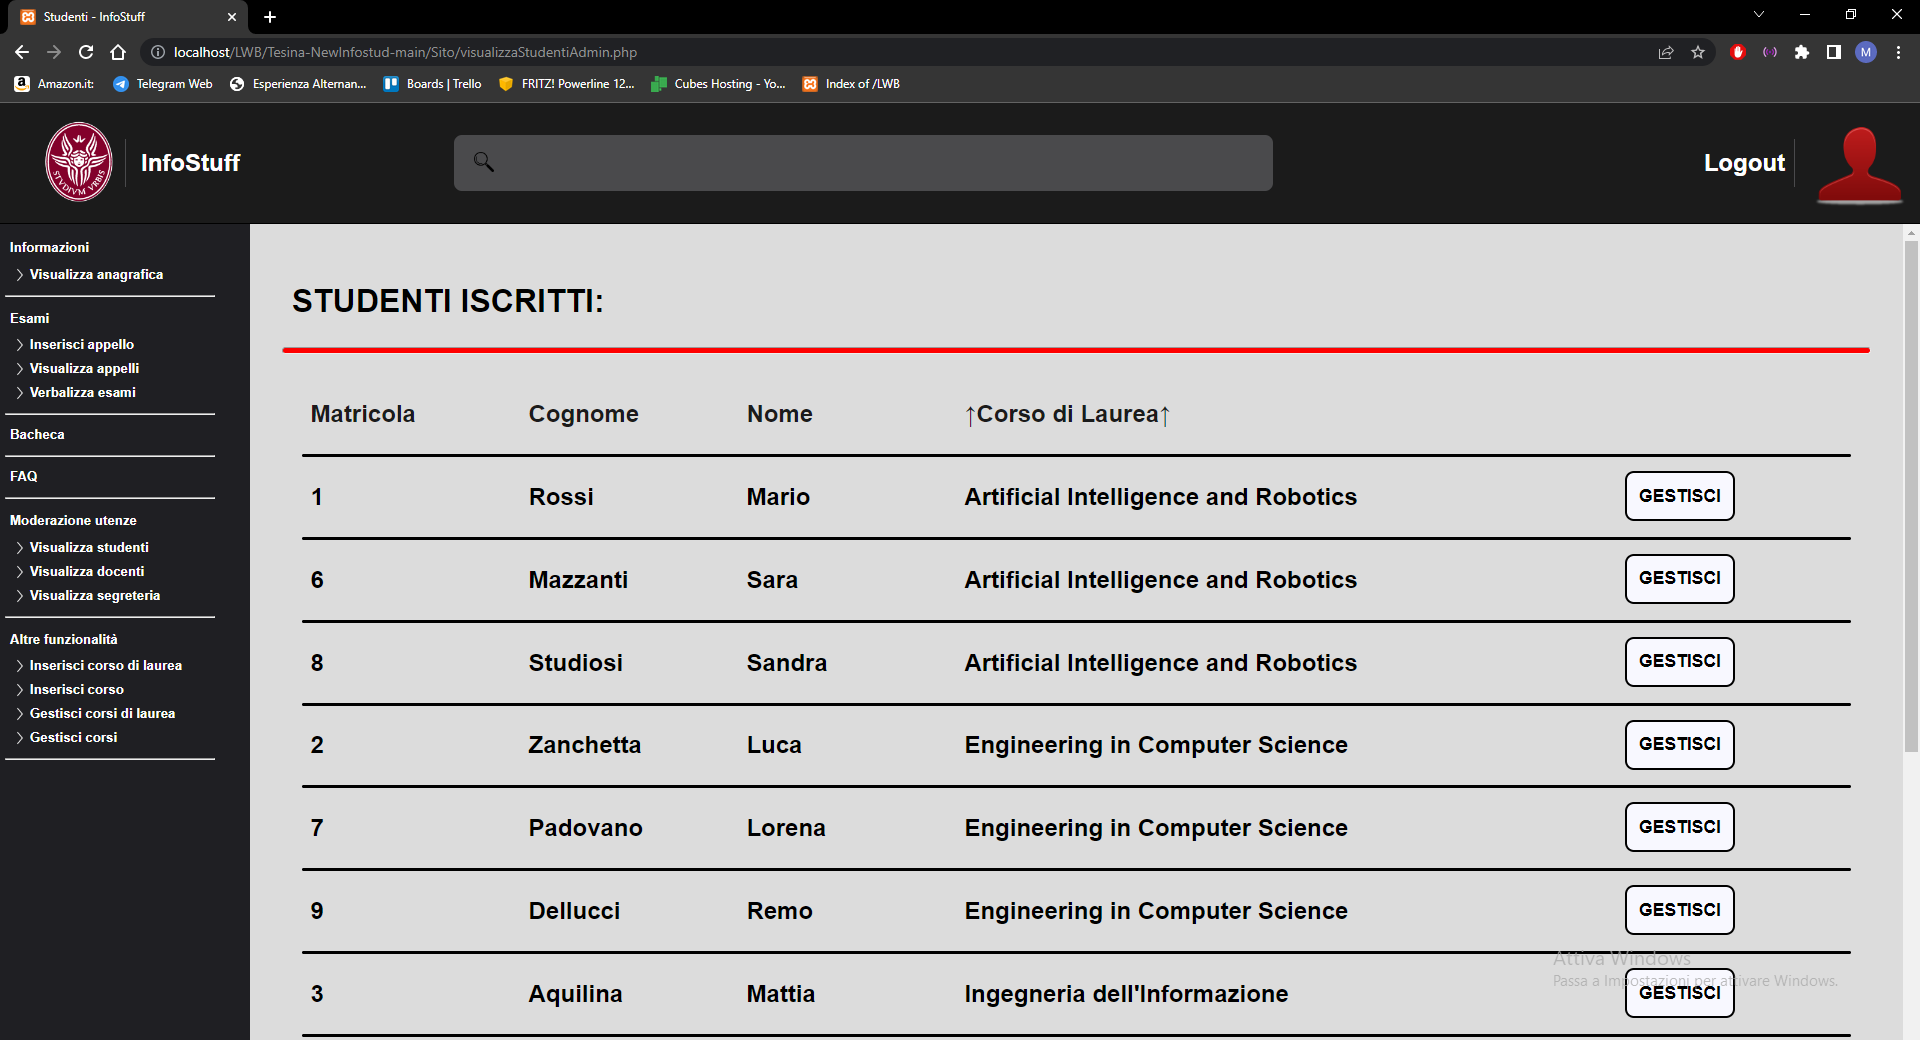
\includegraphics[scale=0.3]{figura2-36.png}
\caption{Visualizzazione dell'elenco delle utenze della tipologia selezionata.}
\end{figure}

Premendo sul pulsante \emph{gestisci}, presente in ogni singola voce dell'elenco di studenti/docenti/segretari mostrato, l'utente amministratore verrà reindirizzato verso una pagina web contenente tutte le informazioni possibili relative all'utenza appena selezionata. Un esempio di tale pagina web è riportato in figura 2.37: come si può notare dalla figura, oltre alle informazioni caratterizzanti l'utenza selezionata, sono presenti tre bottoni: \emph{modifica}, \emph{sospendi} ed \emph{elimina}, rispettivamente per permettere all'amministratore di modificare, sospendere od eliminare l'utenza cui si sta facendo correntemente riferimento.

\begin{figure}
\centering
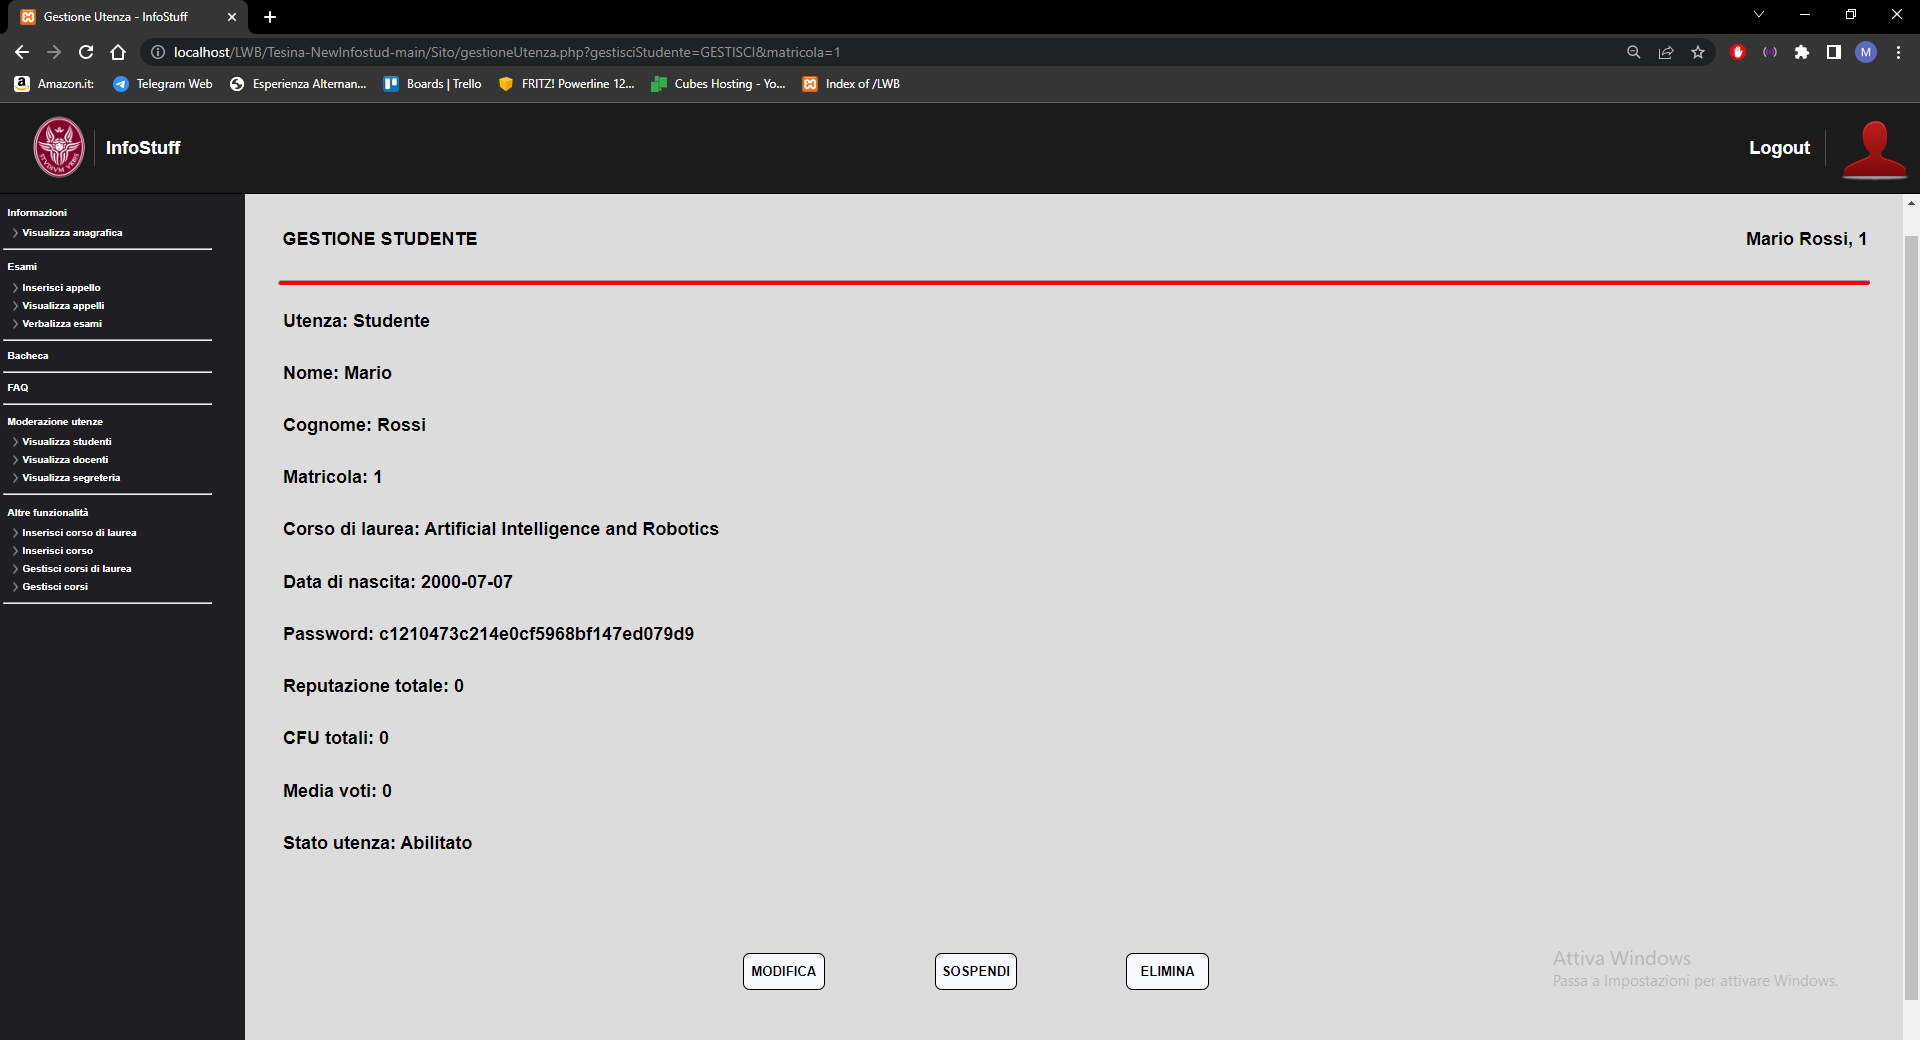
\includegraphics[scale=0.3]{figura2-37.png}
\caption{Pagina di gestione dell'utenza selezionata.}
\end{figure}

\medskip

\subsubsection{Modificare un'utenza}

A partire dalla pagina di gestione dell'utenza, riportata in figura 2.37, premendo sul pulsante \emph{modifica}, l'utente amministratore verrà reindirizzato verso un'opportuna form di modifica dei dati dell'utenza, che naturalmente varia dinamicamente in base al tipo di utenza selezionata e in base alle reali necessità di modifica. Come mostra la figura 2.38, la form di modifica dell'utenza viene mostrata pre-compilata con i dati attuali dell'utenza selezionata, a meno del campo \emph{password}. Qualora il campo password restasse vuoto, la password dell'utenza rimarrebbe invariata; qualora, invece, l'amministratore desiderasse modificare la password dell'utenza (ad esempio, in seguito ad una richiesta esplicita di recupero/modifica password da parte dell'utenza stessa - non entriamo nel dettaglio delle conversazioni private fra utente e amministratore...), basterebbe compilare a piacimento il relativo campo testuale. Gli autori precisano che tale soluzione di modifica della password si è rivelata necessaria poiché, data la non reversibilità dell'algoritmo di cifratura MD5 utilizzato nella crittografia delle password, risulta di fatto impossibile recuperare la reale password dell'utente, per poterla mostrare in chiaro all'amministratore.

\begin{figure}
\centering
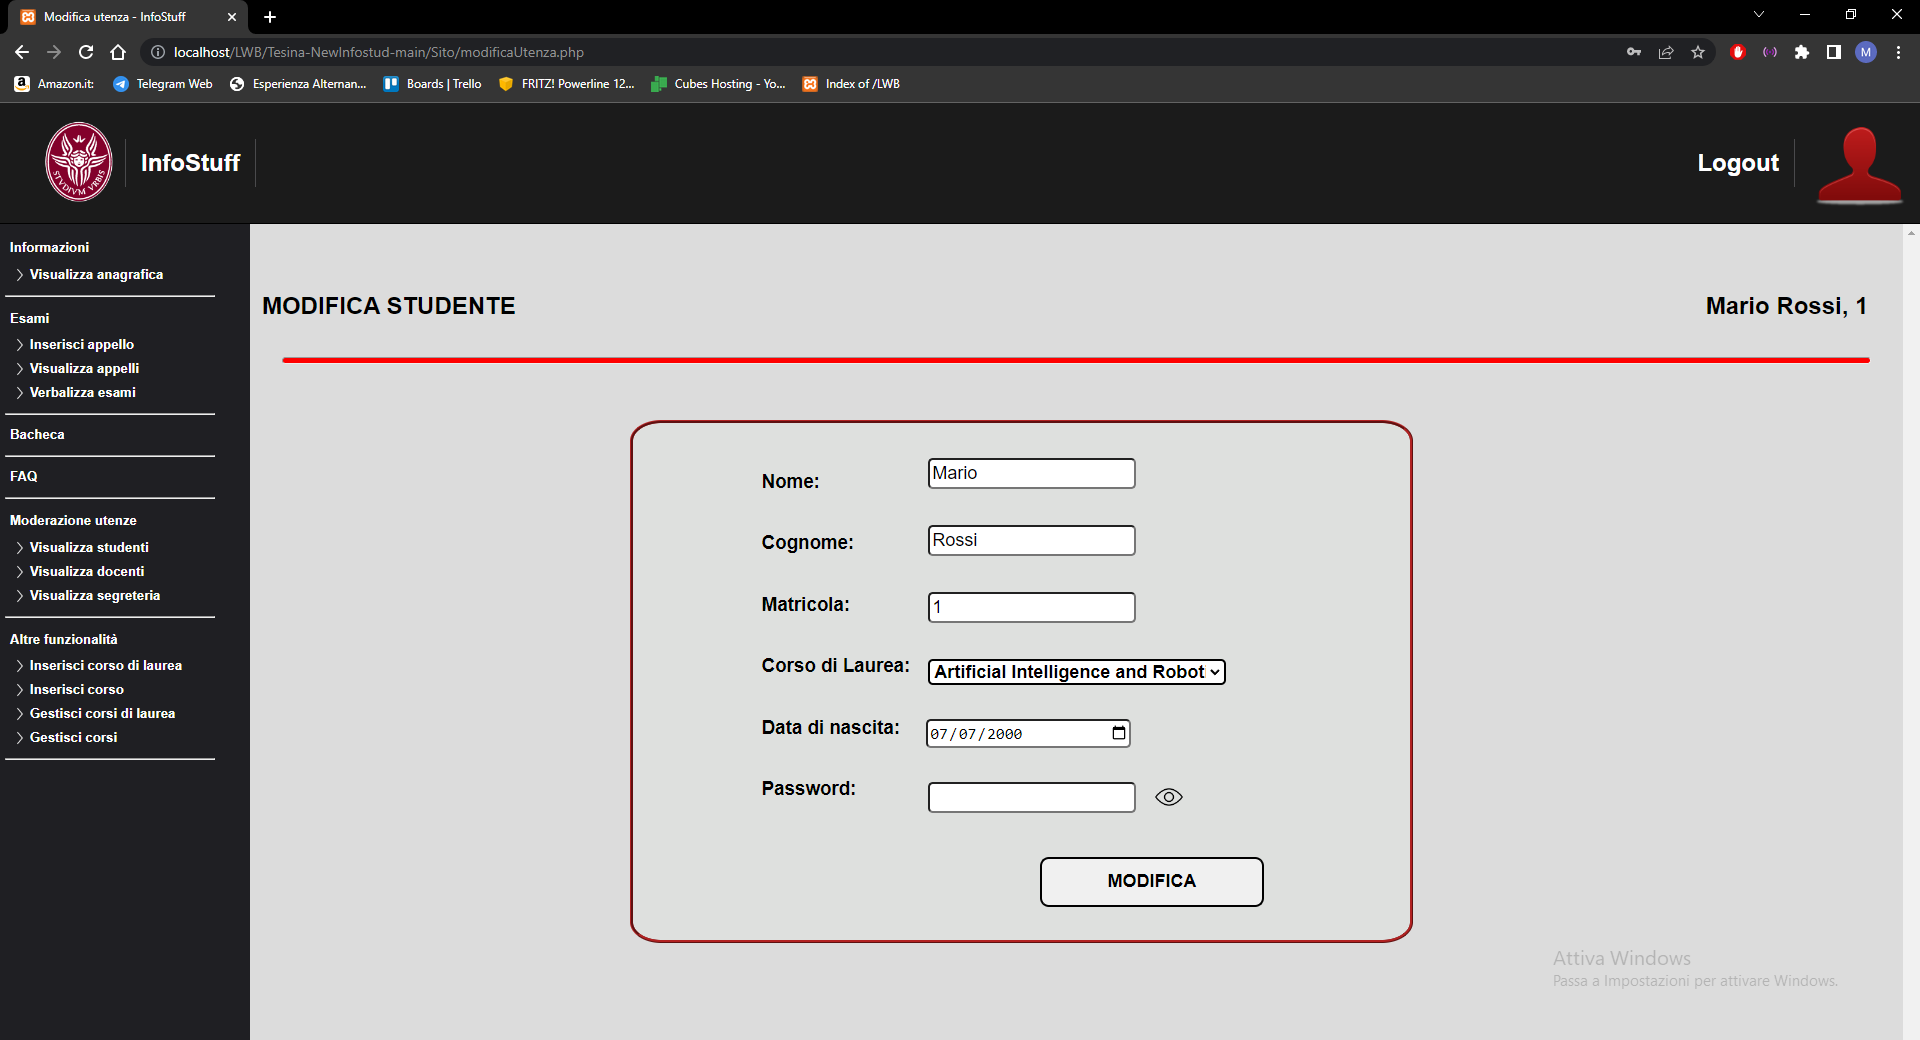
\includegraphics[scale=0.3]{figura2-38.png}
\caption{Form di modifica dell'utenza selezionata.}
\end{figure}

Eventuali errori nella modifica dell'utenza, ad esempio dovuti alla modifica della matricola di uno studente o di un docente o allo username di un segretario (che devono essere univoci!), verranno prontamente segnalati all'utente amministratore, il quale, per poter effettuare la modifica desiderata, dovrà modificare l'inserimento dei dati che hanno generato l'errore.

\medskip

\subsubsection{Sospendere o riabilitare un'utenza}

Supponiamo che l'utenza selezionata sia un'utenza abilitata al pieno utilizzo di tutte le funzionalità messe a disposizione della piattaforma. A partire dalla pagina di gestione dell'utenza, riportata in figura 2.37, premendo sul pulsante \emph{sospendi}, l'utente amministratore scatenerà un processo di sospensione dell'utenza descritto nei dettagli nel capitolo 3 della presente. 

La sospensione di un'utenza può avvenire per svariate ragioni, sostanzialmente a discrezione dell'utente amministratore: pigiando sull'opportuno pulsante, l'utente precedentemente selezionato risulterà sospeso, e il pulsante \emph{sospendi} viene sostituito dal pulsante \emph{riabilita}, come mostrato in figura 2.39.

\begin{figure}
\centering
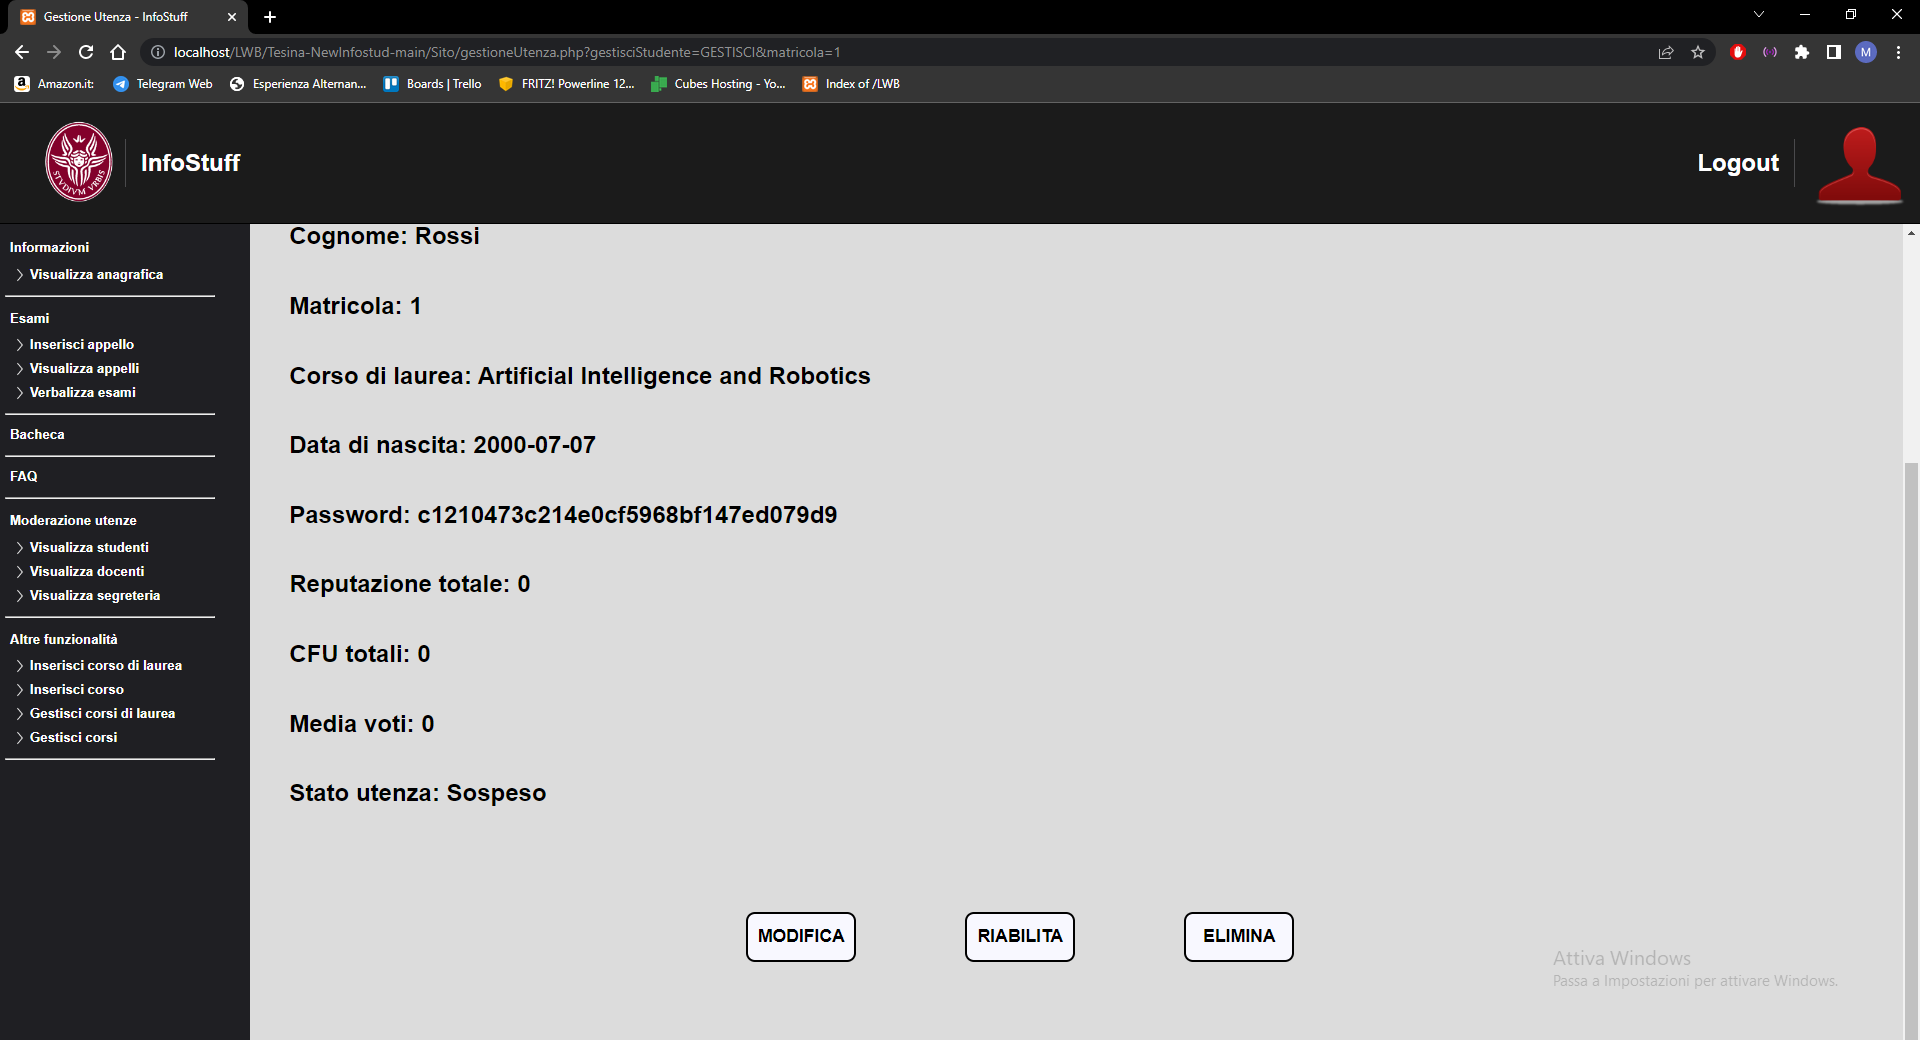
\includegraphics[scale=0.3]{figura2-39.png}
\caption{Gestione di un'utenza sospesa.}
\end{figure}

\emph{Cosa vuol dire sospendere un'utenza?} Ricordiamo al lettore (\emph{cfr. specifiche nel capitolo 1}) che un utente sospeso (sia esso uno studente, un docente od un segretario) non è abilitato ad accedere alle funzionalità extra messe a disposizione dalla piattaforma, ossia l'accesso alle bacheche e alle sezioni delle FAQ, in qualsivoglia loro aspetto e forma. D'altro canto, un utente riabilitato in seguito ad una sospensione ottiene nuovamente il pieno diritto e la piena libertà di accesso alle appena citate funzionalità offerte dalla piattaforma.

\medskip

\subsubsection{Eliminare un'utenza}

A partire dalla pagina di gestione dell'utenza, riportata in figura 2.37, premendo sul pulsante \emph{elimina}, l'utente amministratore scatenerà, dopo opportuna conferma delle proprie intenzioni, un processo di eliminazione dell'utenza precedentemente selezionata, con tutti gli aspetti ad essa relativi. Ad esempio, nel caso dell'eliminazione di uno studente, saranno eliminate anche tutte le informazioni relative alla propria carriera universitaria, così come tutti i suoi dati anagrafici. Tuttavia, a meno che non venga eliminato il relativo corso dalla piattaforma, rimarranno i contributi che lo studente appena eliminato ha apportato nelle bacheche e nelle sezioni FAQ; questi contributi saranno soltanto contrassegnati dall'autore \emph{utente eliminato}, in modo tale che possano continuare ad essere fruibili dalle altre utenze. Un discorso dualmente analogo vale per il caso dell'eliminazione di un docente e di un segretario.

\medskip

\subsection{Inserire un corso di laurea}

A partire da una qualsiasi pagina web relativa all'utenza, è possibile cliccare sulla voce \emph{Inserisci corso di laurea}, sotto la sezione \emph{Altre funzionalità}, all'interno della barra laterale sita a sinistra della pagina stessa. L'utente verrà così reindirizzato ad una pagina web come quella in figura 2.40, nella quale verrà presentata a schermo una form di inserimento di un nuovo corso di laurea. Sostanzialmente, essendo il corso di laurea caratterizzato unicamente da un nome, l'inserimento di un corso di laurea si riduce all'inserimento del suo nome, che deve essere univoco all'interno della piattaforma.

\begin{figure}
\centering
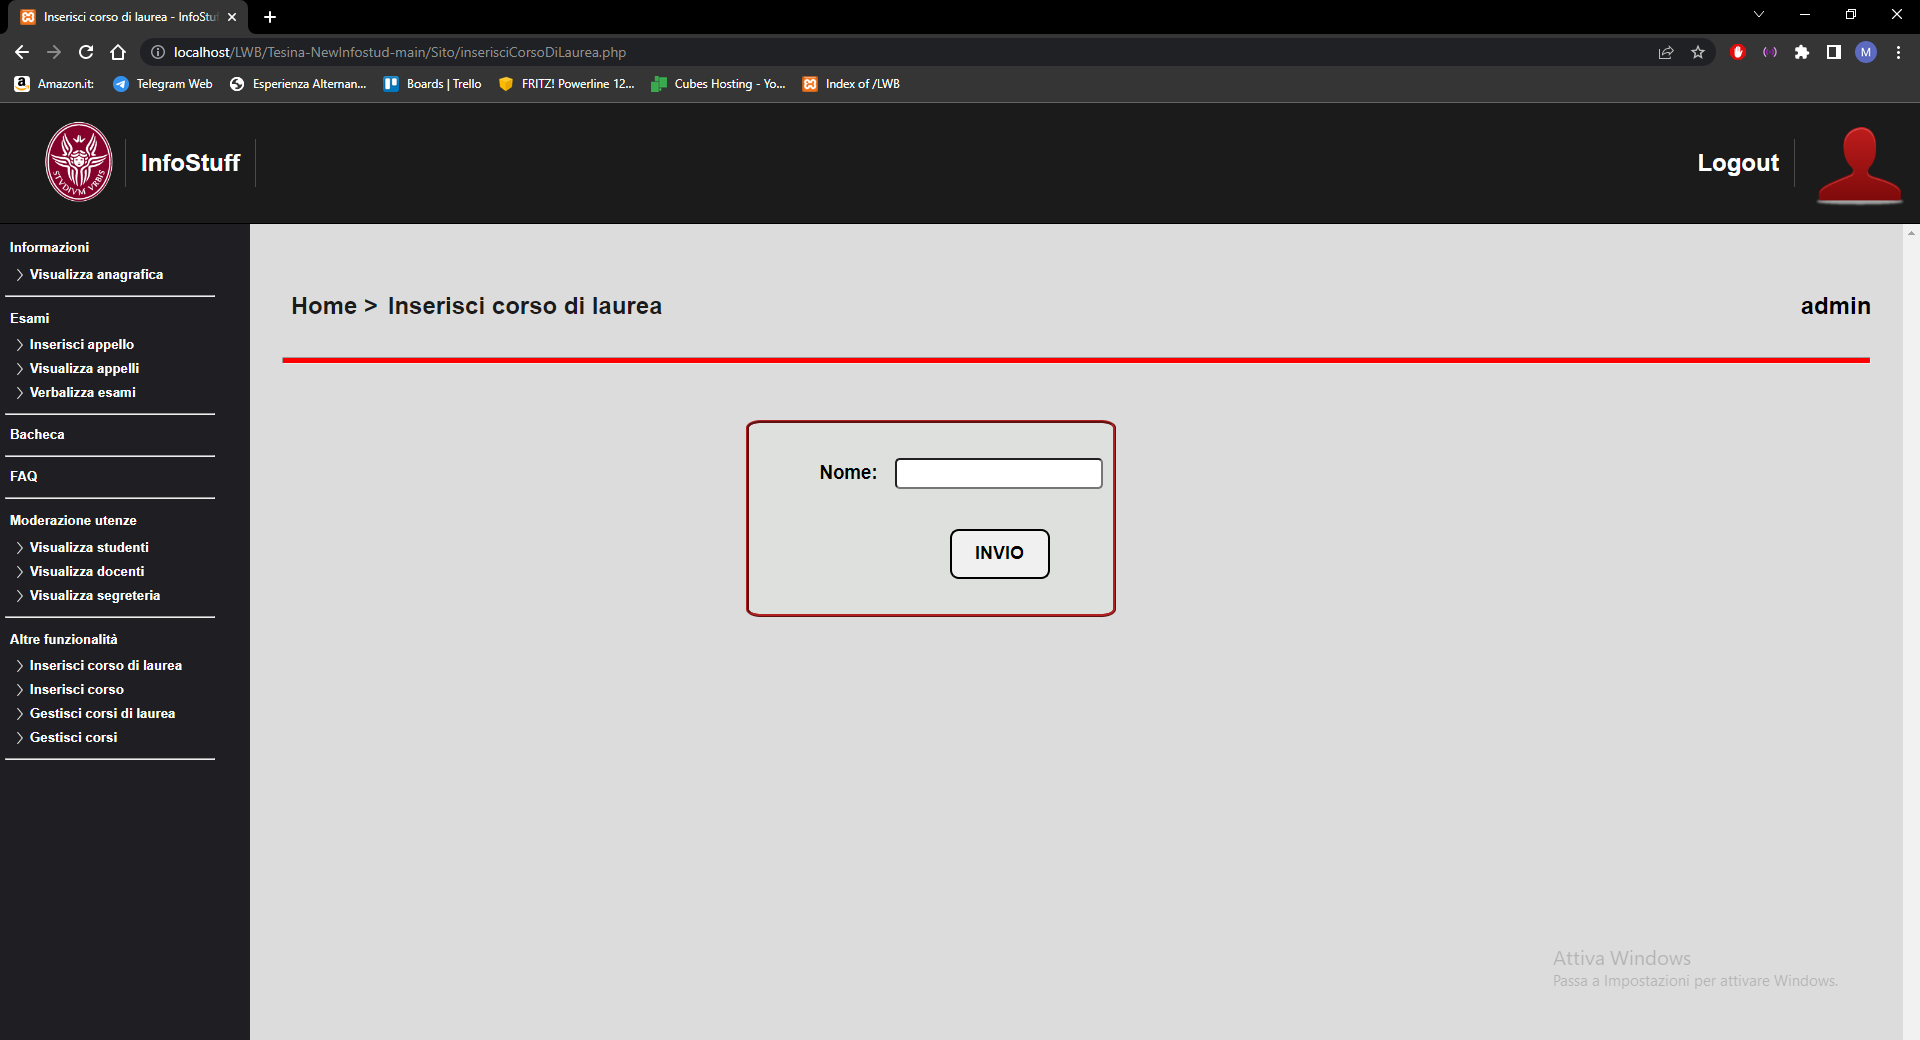
\includegraphics[scale=0.3]{figura2-40.png}
\caption{Form di inserimento di un corso di laurea.}
\end{figure}

\medskip

\subsection{Gestire i corsi di laurea}

A partire da una qualsiasi pagina web relativa all'utenza, è possibile cliccare sulla voce \emph{Gestisci corsi di laurea}, sotto la sezione \emph{Altre funzionalità}, all'interno della barra laterale sita a sinistra della pagina stessa. L'utente verrà così reindirizzato ad una pagina web come quella in figura 2.41, nella quale verranno presentati a schermo tutti i corsi di laurea registrati all'interno della piattaforma.

\begin{figure}
\centering
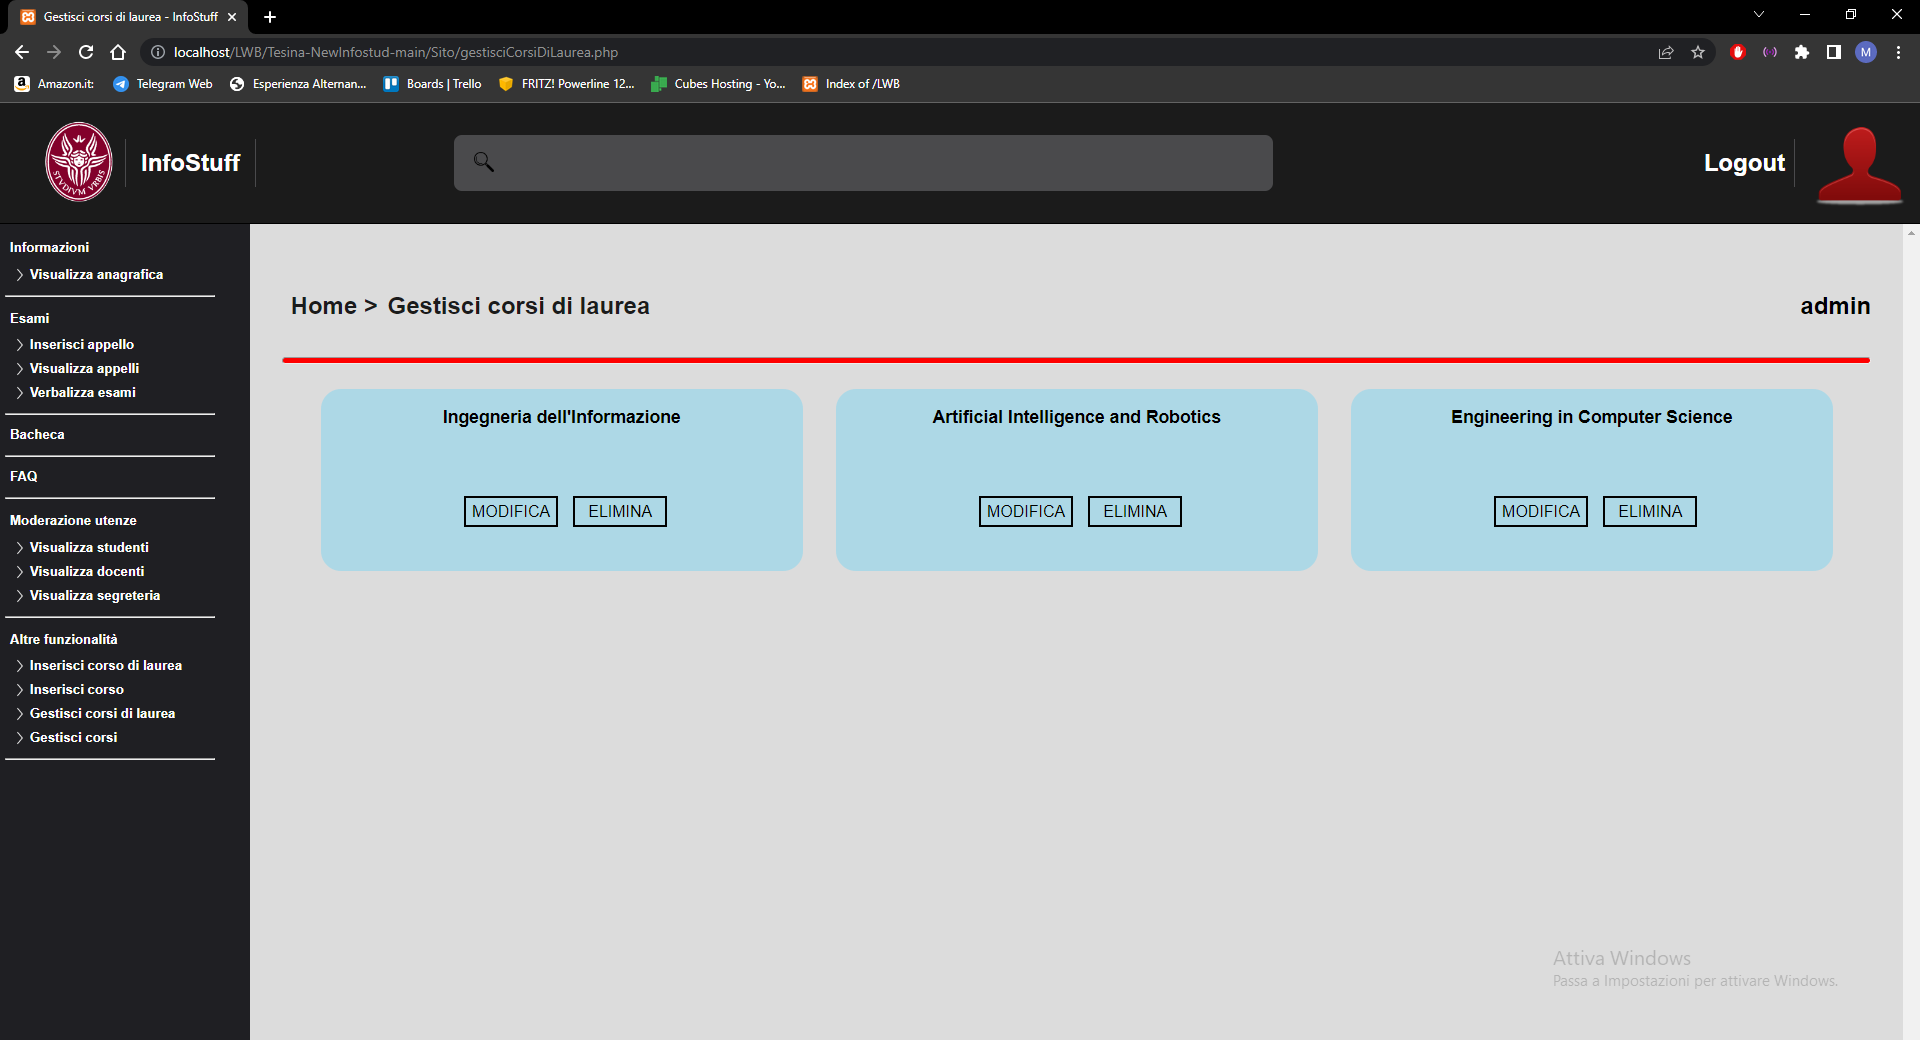
\includegraphics[scale=0.3]{figura2-41.png}
\caption{Visualizzazione di tutti i corsi di laurea registrati presso la piattaforma.}
\end{figure}

Ogni corso di laurea viene presentato in un box contenente il nome del corso di laurea stesso, e due pulsanti: \emph{modifica} ed \emph{elimina}, esattamente come avviene per la visualizzazione degli appelli. Da qui il lettore potrà facilmente intuire le operazioni applicabili al singolo corso di laurea, che verranno in ogni caso approfondite a breve.

\medskip 

\subsubsection{Modificare un corso di laurea}

A partire dalla pagina di gestione dei corsi di laurea, mostrata in figura 2.41, interagendo con il pulsante \emph{modifica}, l'utente amministratore verrà reindirizzato ad una form di modifica del corso di laurea, come mostrato in figura 2.42. La form verrà visualizzata già pre-compilata con i dati del corso di laurea selezionato; l'utente amministratore potrà dunque cambiare il nome del corso di laurea, a patto che questo non sia già presente all'interno dell'insieme dei dati caratterizzanti la piattaforma.

\begin{figure}
\centering
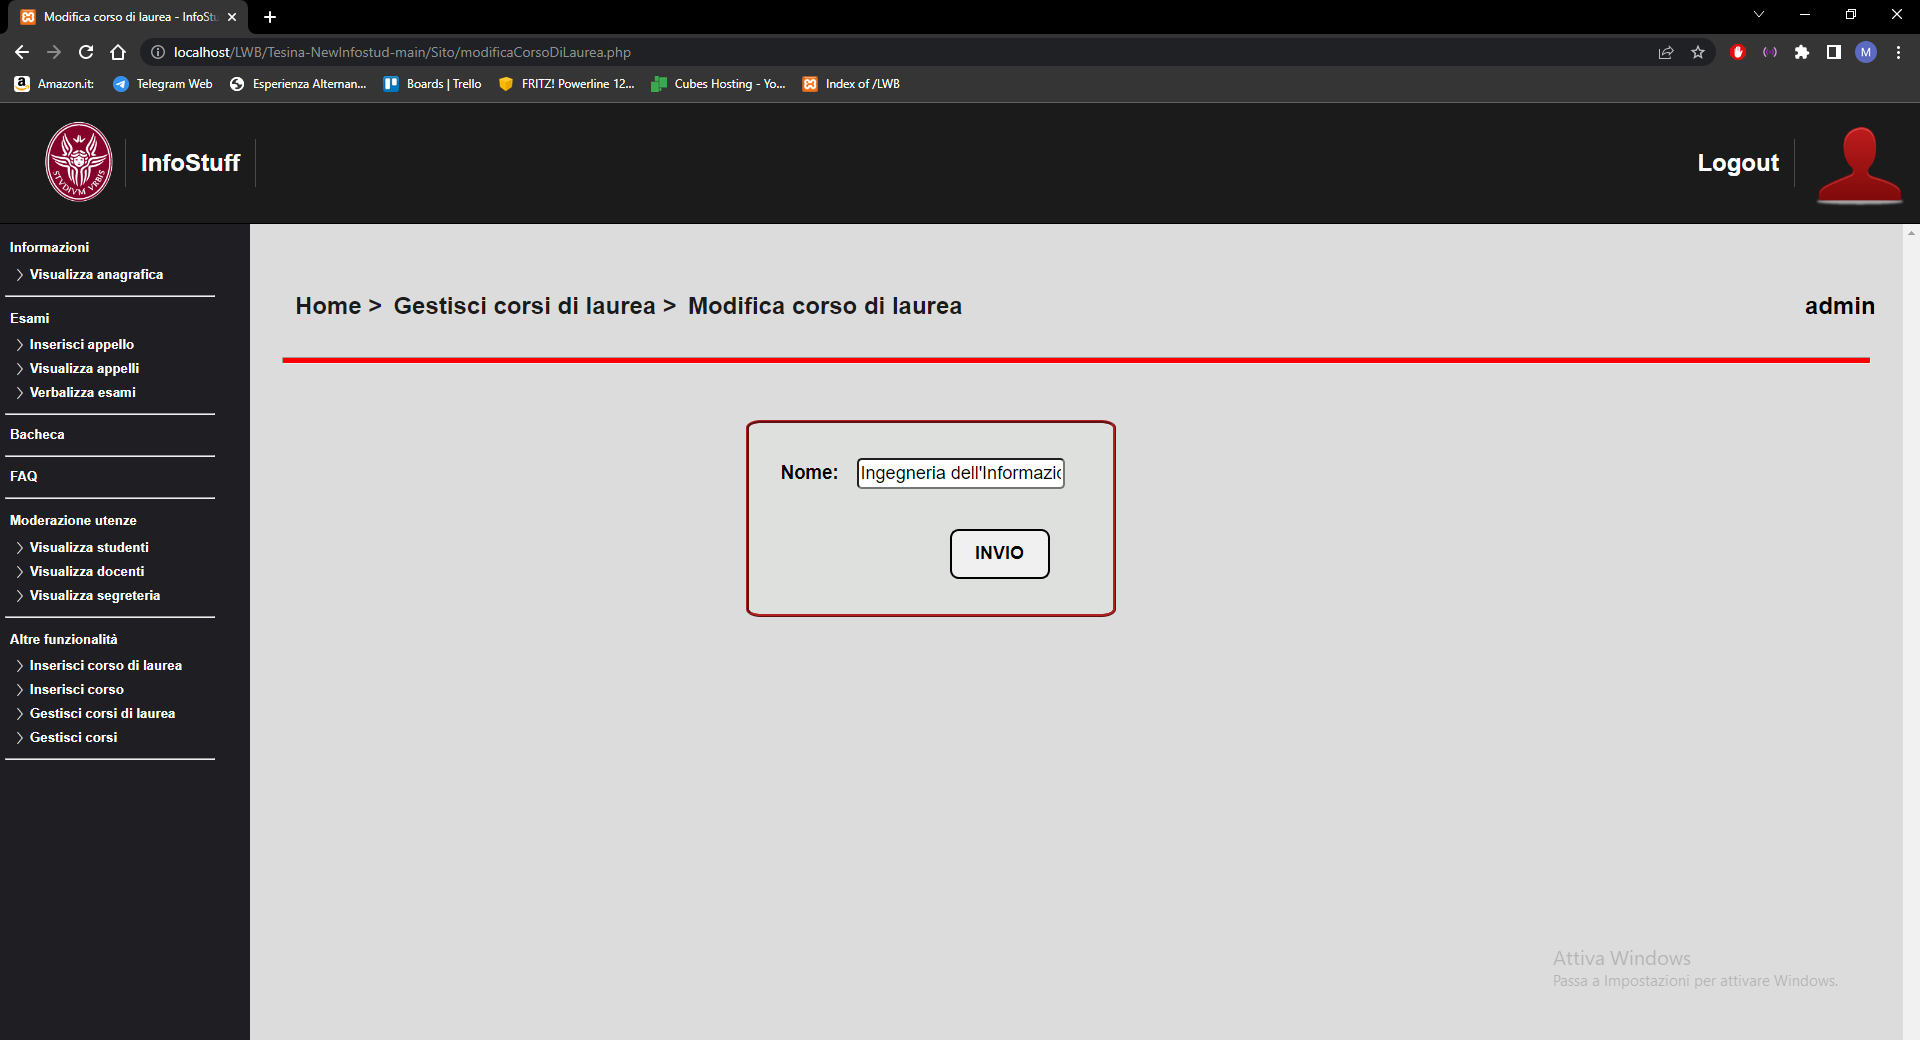
\includegraphics[scale=0.3]{figura2-42.png}
\caption{Form di modifica di un corso di laurea.}
\end{figure}

\medskip

\subsubsection{Eliminare un corso di laurea}

A partire dalla pagina di gestione dei corsi di laurea, mostrata in figura 2.41, interagendo con il pulsante \emph{elimina}, l'utente amministratore scatenerà, dopo opportuna conferma delle proprie intenzioni, un meccanismo di eliminazione del corso di laurea selezionato. Tale meccanismo di eliminazione risulta essere particolarmente delicato: eliminando un corso di laurea, infatti, si sceglie indirettamente di eliminare i dati relativi a tutti i corsi, tutti gli appelli, tutte le bacheche, tutte le sezioni FAQ, tutte le carriere universitarie e tutti gli studenti ad esso relativi. L'utente amministratore, seppur ''onnipotente'' nei confini entro i quali si sviluppa la piattaforma, dovrebbe porre particolare attenzione in questa delicata funzionalità.

\medskip

\subsection{Inserire un corso}

A partire da una qualsiasi pagina web relativa all'utenza, è possibile cliccare sulla voce \emph{Inserisci corso}, sotto la sezione \emph{Altre funzionalità}, all'interno della barra laterale sita a sinistra della pagina stessa. L'utente verrà così reindirizzato ad una pagina web come quella in figura 2.43, nella quale verrà presentata a schermo una form di inserimento di un nuovo corso. Un corso è caratterizzato da un nome, che deve essere univoco entro i limiti di presenza all'interno del corso di laurea cui fa riferimento, da un docente, da un co-docente (opzionale), dall'anno di corso in cui viene erogato, dal semestre in cui viene erogato, dal curriculum cui fa riferimento, dai CFU offerti allo studente dopo il superamento dell'esame che lo caratterizza, da un codice SSD, dal corso di laurea cui fa riferimento e, immancabilmente, da una descrizione che ne permette la fruizione di obiettivi e informazioni.

\begin{figure}
\centering
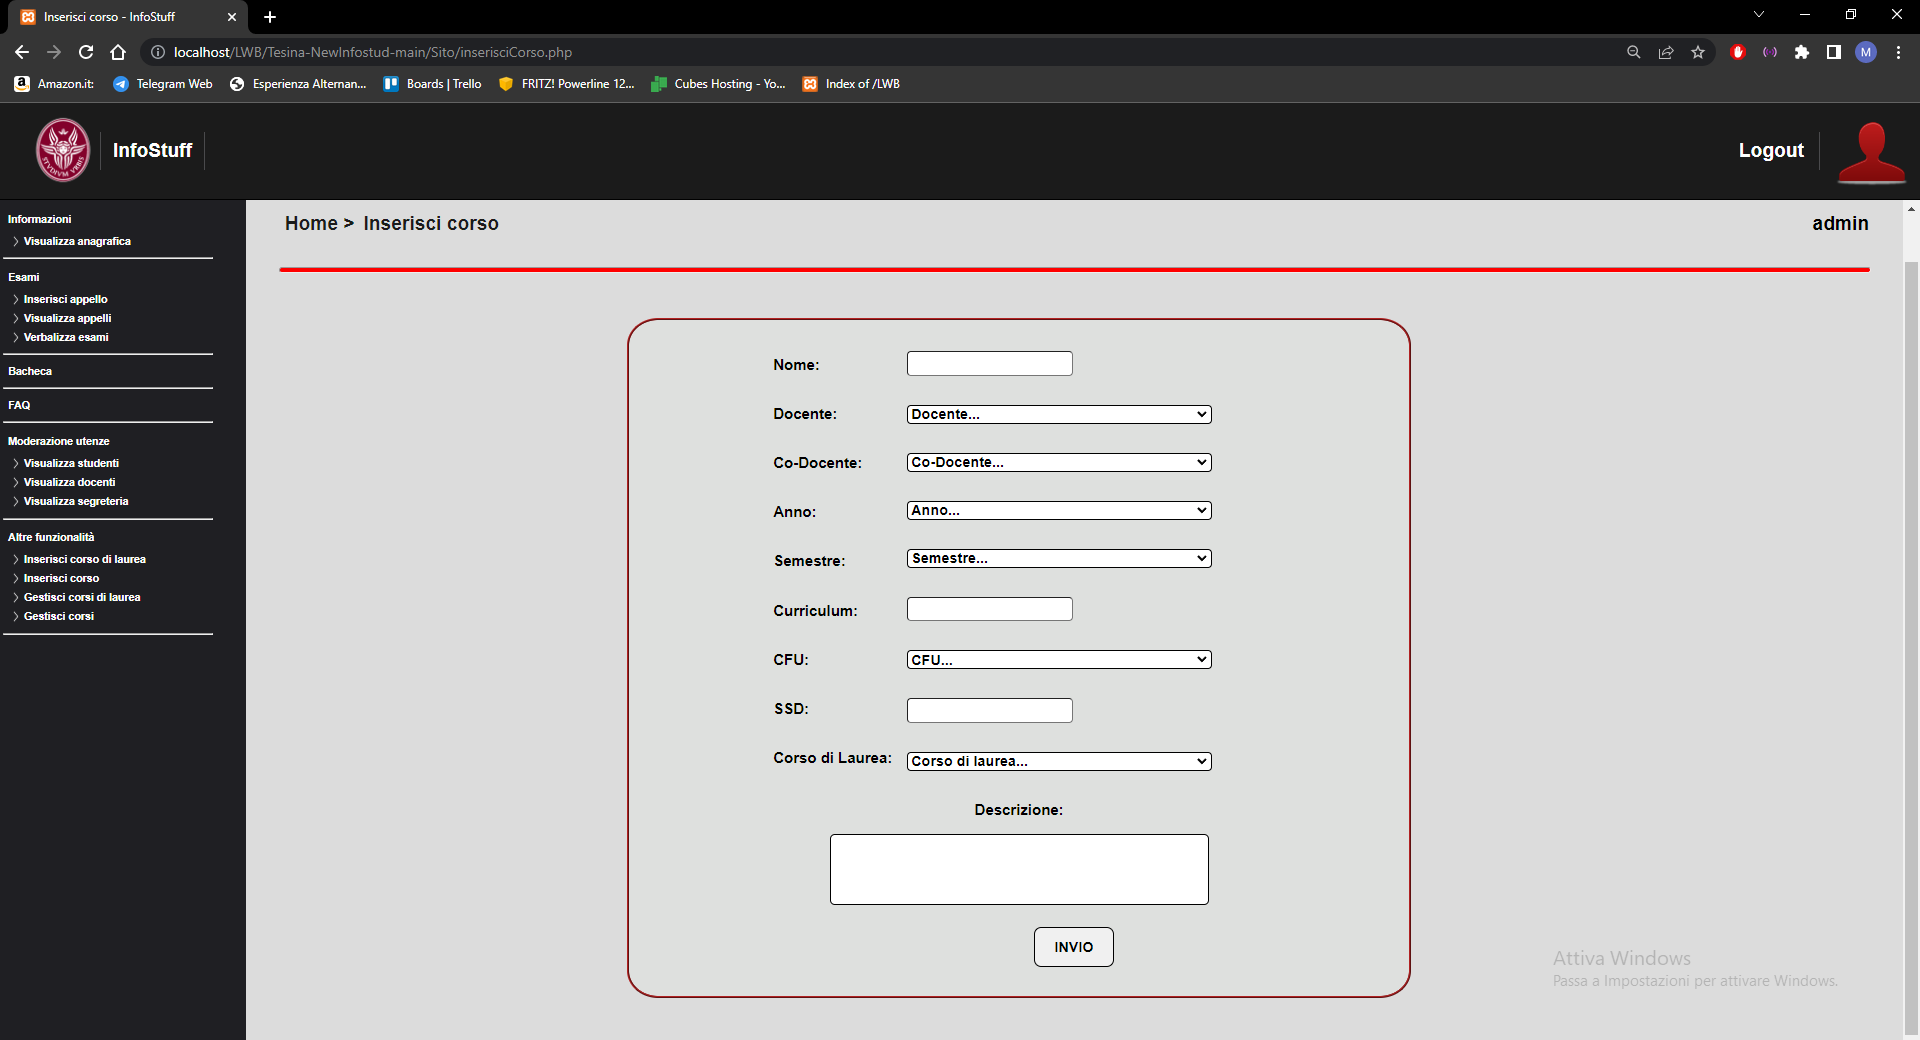
\includegraphics[scale=0.3]{figura2-43.png}
\caption{Form di inserimento di un corso.}
\end{figure}

Specificate tutte queste informazioni, sarà sufficiente premere sul pulsante \emph{invio} per concludere l'operazione di inserimento del corso.

\medskip

\subsection{Gestire i corsi}

A partire da una qualsiasi pagina web relativa all'utenza, è possibile cliccare sulla voce \emph{Gestisci corsi}, sotto la sezione \emph{Altre funzionalità}, all'interno della barra laterale sita a sinistra della pagina stessa. L'utente verrà così reindirizzato ad una pagina web come quella in figura 2.44, nella quale verranno presentati a schermo tutti i corsi relativi a tutti i corsi di laurea registrati all'interno della piattaforma.

\begin{figure}
\centering
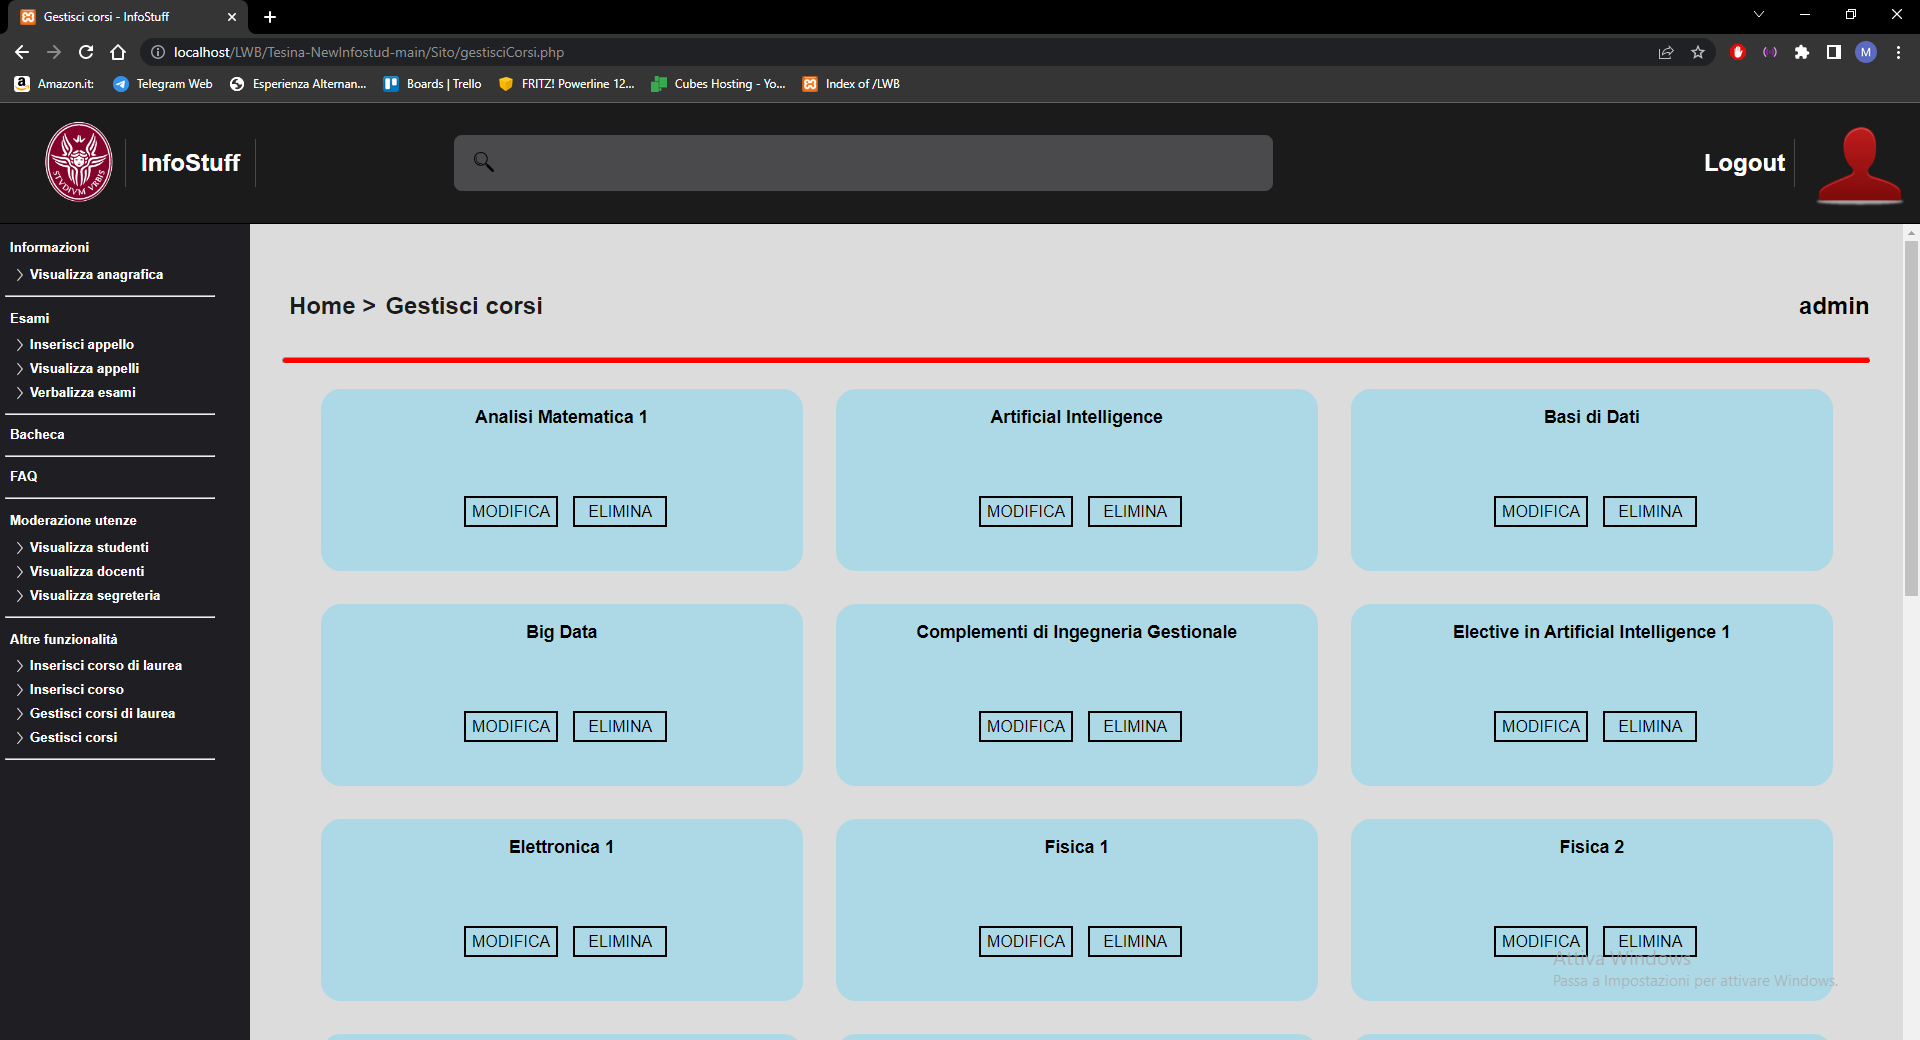
\includegraphics[scale=0.3]{figura2-44.png}
\caption{Visualizzazione di tutti i corsi registrati presso la piattaforma.}
\end{figure}

Ogni corso viene presentato in un box contenente il nome del corso stesso, e due pulsanti: \emph{modifica} ed \emph{elimina}, esattamente come avviene per la visualizzazione degli appelli e dei corsi di laurea. Da qui il lettore potrà facilmente intuire le operazioni applicabili al singolo corso, che verranno in ogni caso approfondite a breve.

\medskip 

\subsubsection{Modificare un corso}

A partire dalla pagina di gestione dei corsi, mostrata in figura 2.44, interagendo con il pulsante \emph{modifica}, l'utente amministratore verrà reindirizzato ad una form di modifica del corso selezionato, come mostrato in figura 2.45. La form verrà visualizzata già pre-compilata con i dati del corso selezionato; l'utente amministratore potrà dunque cambiare i dati a proprio piacimento, a patto che il nome del corso resti univoco all'interno dell'insieme dei corsi relativi al corso di laurea specificato nella form.

\begin{figure}
\centering
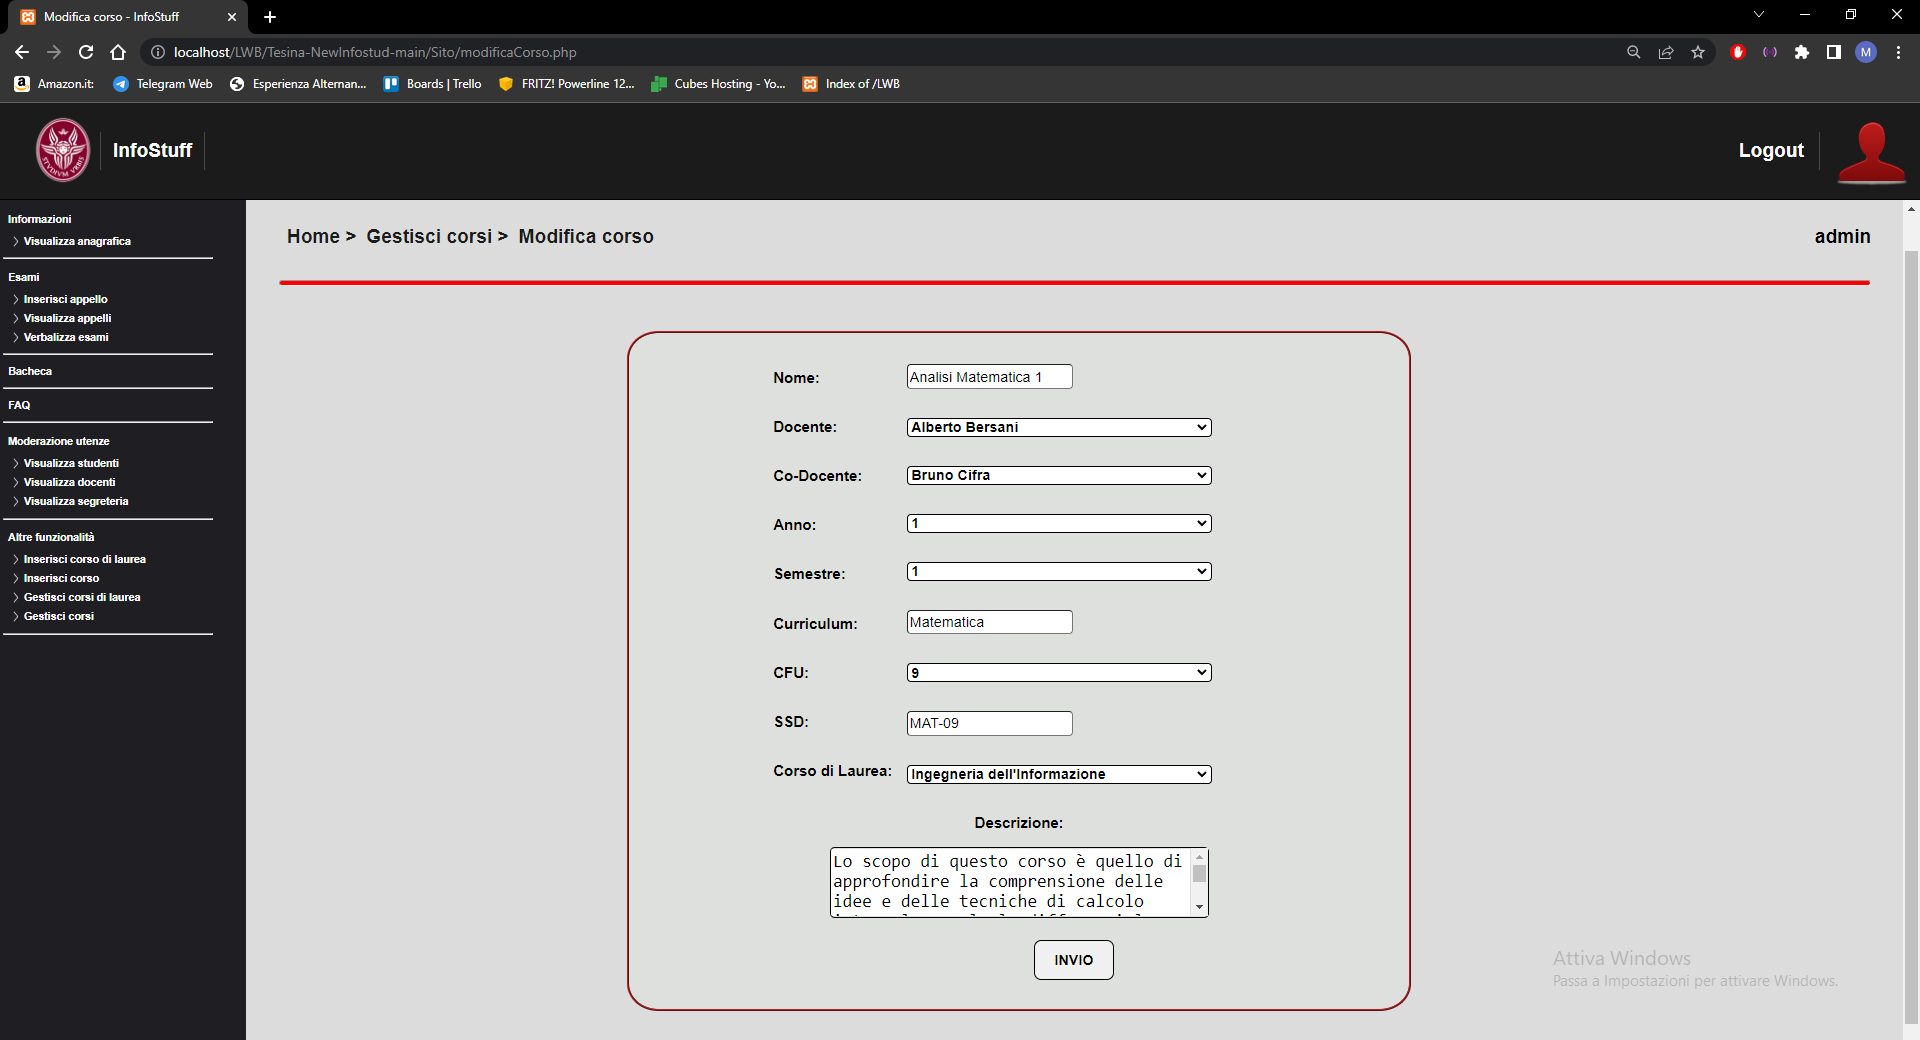
\includegraphics[scale=0.3]{figura2-45.png}
\caption{Form di modifica di un corso.}
\end{figure}

\medskip

\subsubsection{Eliminare un corso di laurea}

A partire dalla pagina di gesione dei corsi, mostrata in figura 2.44, interagendo con il pulsante \emph{elimina}, l'utente amministratore scatenerà, dopo opportuna conferma delle proprie intenzioni, un meccanismo di eliminazione del corso selezionato. L'utente amministratore dovrebbe tenere conto del fatto che eliminando un corso, si sceglie indirettamente di eliminare i dati relativi a tutti gli appelli, tutte le bacheche, tutte le sezioni FAQ e tutte le prenotazioni ad esso relativi. Egli, dunque, seppur ''onnipotente'' nei confini entro i quali si sviluppa la piattaforma, dovrebbe porre particolare attenzione in questa delicata funzionalità.

\medskip
\medskip

\chapter{Programmazione}

In questo capitolo passeremo in rassegna tutti gli script di cui la piattaforma si costituisce, spiegandone il funzionamento. Per facilitarne lo studio separeremo l'insieme del codice in quattro grandi gruppi: l'insieme degli script associati a pagine web, l'insieme degli script che eseguono semplicemente operazioni quali ad esempio inserimenti e cancellazioni, distinguibili dagli ultimi poiché non generano codice xhtml, gli script di definizione, che comprendono le dichiarazioni di strutture dati e funzioni e, in ultimo, gli script dedicati alla definizione dello stile grafico.

\medskip

Per quanto riguarda il terzo gruppo, esso si costituisce per la quasi totalità di script contenti dichiarazioni di funzioni php, il che comporta un'elevata dimensione degli script stessi. Motivo per il quale spiegare il funzionamento di ogni procedura, nelle sezioni dedicate a questi ultimi, risulterebbe di difficile lettura. Si è quindi scelto di esplicare/citare le singole funzioni in tutti quelli script il cui funzionamento dipende dalle ultime.
 
\medskip

\section{Script per pagine web}

Come abbiamo già accennato nell'introduzione, questa sezione sarà dedicata a tutti quegli script associati a pagine web visitabili. Prevedendo molteplici utenze, ciascuna dotata di diverse pagine visitabili, su ciascuna pagina di questo gruppo verrà effettuato un opportuno controllo sulle variabili di sessione assicurando che nessun utente indesiderato raggiunga pagine critiche.

\subsubsection{avvisoCorrispondenze.php}

Questo script realizza una pagina web contenente un avviso che verrà mostrato all'utente qualora si realizzassero delle corrispondenze fra appelli, nell'inserimento o nella modifica degli stessi. La pagina web in questione andrà a chiedere all'utente se, nonostante le corrispondenze avvenute (che vengono mostrate nella parte inferiore della pagina stessa), l'intenzione resta comunque quella di inserire/modificare l'appello che ha generato le corrispondenze in questione. Qualora l'utente rispondesse in modo affermativo, l'inserimento/modifica verrà effettuato/a senza ulteriori indugi; altrimenti, l'utente verrà reindirizzato presso la pagina web di inserimento/modifica dell'appello.

La presenza di eventuali corrispondenze viene calcolata eseguendo la procedura di controllo denominata \emph{verificaProssimità}, disponibile nell'apposito file \emph{phpFunctions-misc.php}.

\medskip

\subsubsection{avvisoErrore.php}

Questo script realizza una pagina web contenente un avviso di errore che verrà mostrato all'utente nelle condizioni opportune, ad esempio nei casi in cui dovessero esserci problemi nell'inserimento di un'entità, nella modifica o nella cancellazione della stessa, e in altre molteplici circostanze. Ogni circostanza viene opportunamente gestita attraverso il set di un cookie contenente il messaggio di errore da mostrare all'utente; una volta mostrato il messaggio, il cookie verrà eliminato dal browser dell'utente. La pagina web, in ultimo, consente all'utente di tornare alla propria homepage, sia essa la homepage di un'utenza autenticata oppure no.

\medskip

\subsubsection{avvisoOK.php}

Questo script realizza una pagina web contenente un avviso di successo che verrà mostrato all'utente nelle condizioni opportune, ad esempio nei casi di inserimento, modifica o cancellazione di un'entità avvenuta in maniera corretta. Nel particolare caso in cui questo script venga chiamato in seguito alla registrazione di uno studente o di un docente presso la piattaforma, verrà stampata anche la matricola generata automaticamente dal sistema, a scopo informativo; il dato viene passato allo script tramite il set di un cookie, come esplicato in precedenza.

\medskip

\subsubsection{form-registrazione.php}

Questo script realizza la funzionalità di registrazione, consentendo all'utente visitatore di creare un account relativo ad un'utenza da lui specificata. Per prima cosa, lo script necessita la ricezione di un campo POST denominato \emph{loginType}, che contiene informazioni sul tipo di utenza di cui si vuole creare l'account. Questo campo viene inviato da una form contenuta nella pagina \emph{login.php} (\emph{si veda a seguire}).

\medskip

La registrazione vera e propria viene gestita da una form che rimanda alla pagina stessa passando i campi necessari per effettuare l'inserimento. In seguito all'invio, lo script effettuerà un controllo sulla presenza dei dati che, in caso di esito positivo, rimanderà l'utente in una pagina di conferma di avvenuta registrazione, descritta poc'anzi.

L'inserimento della nuova utenza avviene utilizzando una delle funzioni contenute in \emph{phpFunctions-insert.php}, in base alla tipologia di utenza selezionata.
 
\medskip

\subsubsection{gestionePrenotazioni.php}

Questo script genera una pagina il cui contenuto dipende dall'utenza, come successivamente vedremo, che in linea di massima mostra un insieme di appelli presenti nel sistema, associando a ciascuno di essi il numero di studenti prenotati e i dettagli su corso e data relativi all'appello stesso. L'accesso alla pagina è vietato agli studenti.

Lo script, dopo aver ricavato informazioni sull'utenza attualmente loggata, genera un contenuto adeguato alla stessa. Più in particolare, qualora l'utenza fosse di tipo amministrativo (\emph{Segreterio} o \emph{Amministratore}), la pagina dovrà contenere tutti gli appelli memorizzati all'interno della piattaforma. A tale scopo, viene utilizzata una funzione denominata \emph{displayFullAppelli}, che genererà il codice necessario allo scopo (\emph{la funzione appartiene alle phpFunctions-display, script che verrà esplicato successivamente}).

Nel caso in cui l'utenza fosse un docente, dovranno essere visualizzati i soli appelli relativi ai corsi di competenza di quest'ultimo. In questi frangenti facciamo affidamento da una seconda procedura denominata \emph{displayAppelliFromCorso}, che verrà eseguita un numero di volte pari al numero di corsi associati al docente, visualizzando così il contenuto richiesto.

\medskip

La pagina è inoltre dotata di una barra di ricerca, realizzata come form rimandante alla pagina stessa. All'atto dell'invio, viene passato un campo denominato \emph{filtro}, rappresentante il contenuto della barra di ricerca. Qualora fosse stato specificato un filtro di visualizzazione tramite la suddetta barra di ricerca, la pagina, dovendo modificare il contenuto, affiderà il compito a due funzioni analoghe a quelle viste sopra che, oltre a ricavare gli appelli, effettuano anche un filtraggio sul nome del corso.

\medskip

\subsubsection{gestioneUtenza.php}

Questo script realizza una pagina web nella quale verrà mostrato un elenco di tutte le informazioni relative ad una certa utenza precedentemente selezionata da un utente amministratore; la visualizzazione dell'elenco suddetto è resa possibile grazie alle opportune funzioni \emph{displayFullStudente}, \emph{displayFullDocente} e \emph{displayFullSegretario}, contenute nell'insieme di funzioni denominato \emph{phpFunctions-display.php}: tali funzioni php raccolgono tutte le informazioni relative all'utenza e le presentano all'utente tramite una echo.

La pagina permette inoltre di reindirizzare l'amministratore verso la modifica dell'utenza selezionata, oppure permette all'amministratore la sospensione, la riabilitazione o l'eliminazione della stessa. L'esecuzione di queste funzionalità può avvenire grazie al passaggio di opportune informazioni attraverso dei campi hidden, passati in POST.

Una nota degna di merito è la seguente: qualora l'amministratore avesse intenzione di proseguire verso l'eliminazione dell'utenza, verrà mostrato a schermo un popup realizzato in Javascript, richiedente conferma delle proprie intenzioni: l'eliminazione, infatti, dovrebbe essere trattata con accortezza.

\medskip

\subsubsection{gestioneCorsi.php}

Questo script realizza una pagina web nella quale verrà mostrato un elenco di tutti i corsi correntemente registrati presso la piattaforma; la visualizzazione dell'elenco suddetto è resa possibile grazie alle opportune funzioni \emph{displayCorsi} e \emph{displayCorsiLike} (nel caso di visualizzazione con filtro di ricerca), contenute nell'insieme di funzioni denominato \emph{phpFunctions-display.php}: tali funzioni php raccolgono le informazioni relative ai corsi registrati e le presentano all'utente tramite una echo in dei riquadri azzurri. L'effetto è realizzato tramite alcune regole di stile contenute principalmente nel file \emph{stile-base.css}, descritto in seguito.

La pagina permette inoltre di reindirizzare l'amministratore verso la modifica o l'eliminazione di un particolare corso selezionato; l'esecuzione di queste funzionalità può avvenire grazie al passaggio di opportune informazioni attraverso dei campi hidden, passati in POST.

Una nota degna di merito è la seguente: qualora l'amministratore avesse intenzione di proseguire verso l'eliminazione di un corso, verrà mostrato a schermo un popup realizzato in Javascript, richiedente conferma delle proprie intenzioni: l'eliminazione, infatti, dovrebbe essere trattata con accortezza.

\medskip

\subsubsection{gestioneCorsiDiLaurea.php}

Questo script realizza una pagina web nella quale verrà mostrato un elenco di tutti i corsi di laurea correntemente registrati presso la piattaforma; la visualizzazione dell'elenco suddetto è resa possibile grazie alle opportune funzioni \emph{displayCorsiDiLaurea} e \emph{displayCorsiDiLaureaLike} (nel caso di visualizzazione con filtro di ricerca), contenute nell'insieme di funzioni denominato \emph{phpFunctions-display.php}: tali funzioni php raccolgono le informazioni relative ai corsi di laurea registrati e le presentano all'utente tramite una echo in dei riquadri azzurri. L'effetto è realizzato tramite alcune regole di stile contenute principalmente nel file \emph{stile-base.css}, descritto in seguito.

La pagina permette inoltre di reindirizzare l'amministratore verso la modifica o l'eliminazione di un particolare corso di laurea selezionato; l'esecuzione di queste funzionalità può avvenire grazie al passaggio di opportune informazioni attraverso dei campi hidden, passati in POST.

Una nota degna di merito è la seguente: qualora l'amministratore avesse intenzione di proseguire verso l'eliminazione di un corso, verrà mostrato a schermo un popup realizzato in Javascript, richiedente conferma delle proprie intenzioni: l'eliminazione, infatti, dovrebbe essere trattata con accortezza.

\medskip

\subsubsection{homepage-bacheca.php}

Questo script realizza una pagina web nella quale, dipendentemente dall'utenza autenticata, verrà mostrato un elenco di tutti i corsi aventi una sezione bacheca; la visualizzazione dell'elenco suddetto è resa possibile grazie ad un ciclo sui vari corsi da visualizzare, che vengono determinati dalla funzione \emph{getCorsi}, nel caso in cui fosse autenticata un'utenza amministrativa, o dalla funzione \emph{getCorsiFromCorsoDiLaurea}, nel caso in cui fosse autenticato uno studente iscritto ad un corso di laurea. Entrambe le funzioni sono contenute nell'insieme di funzioni denominato \emph{phpFunctions-get.php}. L'effetto di visualizzazione dei corsi suddetti è realizzato tramite alcune regole di stile contenute nel file \emph{stileVisualizzazioneLista.css}, descritto in seguito.

La pagina permette inoltre di reindirizzare l'utente verso la bacheca del singolo corso selezionato, grazie al passaggio di opportune informazioni attraverso dei campi hidden, passati in POST. Una nota degna di merito è la seguente: qualora l'utenza autenticata fosse stata sospesa da un'utenza amministrativa, lo script impedirà l'accesso alla visualizzazione dei corsi sopra esplicata, e verrà mostrato a schermo un popup realizzato in Javascript indicante l'impossibilità di accedere a tale sezione della piattaforma. Il controllo sulla sospensione viene realizzato tramite un controllo sulla flag di stato dell'utenza autenticata, non appena essa dovesse venire reindirizzata al presente script.

\medskip


\subsubsection{homepage-faq.php}

Questo script realizza una pagina web nella quale, dipendentemente dall'utenza autenticata, verrà mostrato un elenco di tutti i corsi aventi una sezione FAQ; la visualizzazione dell'elenco suddetto è resa possibile grazie ad un ciclo sui vari corsi da visualizzare, che vengono determinati dalla funzione \emph{getCorsi}, nel caso in cui fosse autenticata un'utenza amministrativa, o dalla funzione \emph{getCorsiFromCorsoDiLaurea}, nel caso in cui fosse autenticato uno studente iscritto ad un corso di laurea. Entrambe le funzioni sono contenute nell'insieme di funzioni denominato \emph{phpFunctions-get.php}. L'effetto di visualizzazione dei corsi suddetti è realizzato tramite alcune regole di stile contenute nel file \emph{stileVisualizzazioneLista.css}, descritto in seguito.

La pagina permette inoltre di reindirizzare l'utente verso la sezione FAQ del singolo corso selezionato, grazie al passaggio di opportune informazioni attraverso dei campi hidden, passati in POST. Una nota degna di merito è la seguente: qualora l'utenza autenticata fosse stata sospesa da un'utenza amministrativa, lo script impedirà l'accesso alla visualizzazione dei corsi sopra esplicata, e verrà mostrato a schermo un popup realizzato in Javascript indicante l'impossibilità di accedere a tale sezione della piattaforma. Il controllo sulla sospensione viene realizzato tramite un controllo sulla flag di stato dell'utenza autenticata, non appena essa dovesse venire reindirizzata al presente script.

\medskip

\subsubsection{homepage-users-appelliPrenotati.php}

Questo script realizza una pagina web nella quale verrà mostrato un elenco di tutte le prenotazioni relative agli appelli effettuate dallo studente autenticato nella sessione corrente; la visualizzazione dell'elenco suddetto è resa possibile grazie ad un ciclo sulle varie prenotazioni da visualizzare, che vengono determinate dalla funzione \emph{getPrenotazioniStudente}. Per ogni prenotazione trovata, viene determinato l'appello di afferenza e il relativo corso di riferimento, grazie alle due funzioni \emph{getAppelloFromId} e \emph{getCorsoById}; la singola voce sarà costituita dal nome del corso, dalla data dell'appello e da un pulsante di annullamento della prenotazione. Le funzioni citate sono contenute nell'insieme di funzioni denominato \emph{phpFunctions-get.php}. L'effetto di visualizzazione dei corsi suddetti è realizzato tramite alcune regole di stile contenute nel file \emph{stileVisualizzazioneLista.css}, descritto in seguito.

La pagina permette, come già citato, di annullare in qualsiasi momento una prenotazione effettuata; ciò è viene reso possibile dall'esecuzione dello script \emph{eliminaPrenotazioneAppello-script.php}, descritto in seguito, al quale viene passata l'informazione circa l'id della prenotazione da eliminare attraverso un campo hidden, passato in POST.

\medskip

\subsubsection{homepage-users-Carriera.php}

Questo script realizza una pagina web accessibile dalla sola utenza \emph{studente}, nella quale verrà mostrato un elenco di tutte le informazioni relative alla carriera universitaria dello studente autenticato nella sessione corrente; la visualizzazione dell'elenco suddetto è resa possibile grazie all'opportuna funzione \emph{displayCarrieraStudente}, contenuta nell'insieme di funzioni denominato \emph{phpFunctions-display.php}: tale funzione php raccoglie le informazioni relative alla carriera universitaria dello studente ricevuto come parametro, e le presenta all'utente tramite una echo.

Più in dettaglio, verranno presentate all'utente le seguenti informazioni: corso di laurea di riferimento, reputazione totale, numero totale dei CFU acquisiti e media dei voti relativi agli esami sostenuti.

\medskip

\subsubsection{homepage-users-esamiSostenuti.php}

Questo script realizza una pagina web accessibile dalla sola utenza \emph{studente}, nella quale verrà mostrato un elenco di tutte le informazioni relative agli esami sostenuti dallo studente autenticato nella sessione corrente; la visualizzazione dell'elenco suddetto è resa possibile grazie all'esecuzione di un ciclo su una lista di esami sostenuti dallo studente, ottenibile mediante l'esecuzione della funzione \emph{getEsamiSostenuti}. Per ogni esame sostenuto contenuto in questa lista, si ottengono informazioni relative all'appello di riferimento (tramite la funzione \emph{getAppelloFromId}), al relativo corso (tramite la funzione \emph{getCorsoById}) e alla data in cui lo studente ha svolto l'esame. Le funzioni appena citate sono tutte contenute nell'insieme di funzioni denominato \emph{phpFunctions-get.php}. L'effetto di visualizzazione dei suddetti esami sostenuti è realizzato tramite alcune regole di stile contenute nel file \emph{stileVisualizzazioneLista.css}, descritto in seguito.

Più in dettaglio, verranno presentate all'utente le seguenti informazioni: nome del corso del quale si è sostenuto l'esame, data di svolgimento dell'esame ed esito complessivo (verbalizzato) dell'esame stesso.

\medskip

\subsubsection{homapage-users-prenotaAppello.php}

Questo script realizza una pagina web accessibile unicamente da parte dell'utenza \emph{studente}, nella quale verrà mostrato un elenco di tutti gli appelli prenotabili da parte dello studente autenticato nella sessione corrente; la visualizzazione dell'elenco suddetto è resa possibile grazie alla funzione \emph{displayAppelliPrenotabili}, contenuta nell'insieme di funzioni denominato \emph{phpFunctions-display.php}: tale funzione php raccoglie le informazioni relative agli appelli prenotabili da parte dello studente autenticato nella sessione corrente, e le presenta all'utente tramite una echo in dei riquadri azzurri. L'effetto è realizzato tramite alcune regole di stile contenute principalmente nel file \emph{stile-base.css}, descritto in seguito.

Per \emph{appello prenotabile} si intende un appello non ancora prenotato, relativo ad un corso del quale non si sia ancora sostenuto un esame che abbia avuto esito positivo. La pagina permette, tramite un opportuno pulsante \emph{prenota} sito all'interno del singolo riquadro azzurro dell'appello di interesse, di rendere possibile allo studente la prenotazione di un qualsiasi appello fra quelli mostrati: interagendo con tale pulsante, infatti, verrà eseguito lo script \emph{prenotaAppello-script.php}, al quale, per poter completare l'opera di prenotazione, vengono passate le informazioni relative alla matricola dello studente autenticato nella sessione corrente e l'id dell'appello selezionato, tramite opportuni campi hidden inviati in POST. Il funzionamento specifico di tale script sarà approfondito nel seguito.

\medskip

\subsubsection{homapage-users-visualizzaBacheca.php}

Questo script realizza una pagina web non accessibile all'utenza \emph{docente}, nella quale verrà mostrato un elenco di tutti i post contenuti nella bacheca relativa al corso selezionato nella pagina generata dallo script \emph{homepage-bacheca.php}: tale pagina è accessibile unicamente da utenze \textbf{non sospese}. La visualizzazione dell'elenco suddetto è resa possibile grazie all'esecuzione di un ciclo su una lista di post relativi alla bacheca del corso selezionato, ottenibile mediante l'esecuzione della funzione \emph{getListaPost}. 

La lista dei post viene visualizzata in modo particolare: vengono fissati in cima i due post aventi la maggiore utilità, seguiti da tutti gli altri, visualizzati cinque per volta; è possibile cambiare pagina di visualizzazione da un piccolo menù di pagine sito in cima alla lista dei post, realizzato dinamicamente con dei bottoni submit in base al numero totale dei post da visualizzare; un campo hidden mantiene memoria del numero della pagina correntemente in visualizzazione. I post, inoltre, possono essere riordinati secondo differenti criteri: per numero di repliche, per utilità o per data di pubblicazione; sarà sufficiente premere sugli appositi pulsanti presenti in cima alla lista; questi reindirizzano l'utente alla pagina stessa, che questa volta disporrà di un'informazione di visualizzazione passata in POST tramite un opportuno campo hidden. Per ogni post contenuto in questa lista, si potranno visualizzare le informazioni relative al titolo, all'autore, al numero di repliche, all'utilità totale e alla data di pubblicazione del post stesso. Le funzioni appena citate sono tutte contenute nell'insieme di funzioni denominato \emph{phpFunctions-get.php}. 

Interagendo con un qualsiasi post, l'utente verrà reindirizzato verso una pagina di visualizzazione del post stesso, creata dallo script \emph{homepage-users-visualizzaPost}, alla quale vengono passate le opportune informazioni in GET attraverso dei campi hidden. Inoltre, la pagina rende disponibile una funzionalità di creazione di un post: interagendo con l'apposito pulsante \emph{crea post}, infatti, verrà eseguita una funzione Javascript in grado di rendere visibile la form di inserimento di un nuovo post. L'effetto di visualizzazione del suddetto elenco di post è realizzato tramite alcune regole di stile contenute nel file \emph{stileBacheca.css}, descritto in seguito.

\medskip

\subsubsection{homapage-users-visualizzaFaq.php}

Questo script realizza una pagina web relativa alla sezione FAQ inerente al corso selezionato nella pagina generata dallo script \emph{homepage-faq.php}; in questa pagina verranno mostrati due blocchi principali: il primo è costituito da una lista di domande a cui è stata già data una risposta, mentre il secondo è costituito da una lista di domande a cui, invece, non è ancora stata data alcuna risposta. Tale pagina è accessibile unicamente da utenze \textbf{non sospese}. La visualizzazione dei suddetti blocchi è resa possibile grazie all'esecuzione di due cicli: il primo su una lista di FAQ complete, il secondo su una lista di FAQ incomplete, entrambe relative alla sezione FAQ del corso selezionato. Queste due liste sono ottenibili mediante l'esecuzione delle funzioni \emph{getFaqComplete} e \emph{getFaqIncomplete}; le funzioni appena citate sono tutte contenute nell'insieme di funzioni denominato \emph{phpFunctions-get.php}. 

La singola FAQ (coppia domanda-risposta) è accompagnata da un voto di utilità totale, calcolato a partire dalla somma algebrica di tutti i voti di \emph{up (+1)} e \emph{down (-1)} ricevuti dalla FAQ stessa, da parte di altre utenze. Tale voto è racchiuso fra due frecce, realizzate con due image submit buttons: tramite queste frecce, uno studente autenticato nella sessione corrente è in grado di votare tutte le FAQ di cui non è autore. Oltre alla funzionalità di voto, uno studente può proporre nuove domande, grazie ad una form visualizzabile nella parte inferiore della pagina web.

Un'utenza di tipo \emph{docente} è in grado di poter modificare od eliminare tutte le FAQ (complete e incomplete) relative alle sole sezioni FAQ di propria competenza, ossia alle sezioni FAQ relative a corsi da egli impartiti. Premendo sull'apposita icona di eliminazione (facilmente identificabile: è a forma di cestino), un docente scatenerà l'eliminazione, dopo opportuna conferma delle proprie intenzioni, della FAQ selezionata: ciò è possibile grazie all'esecuzione dello script \emph{deleteFaq.php}, approfondito in seguito. Premendo invece sull'apposita  icona di modifica (facilmente identificabile: è a forma di matita), un docente scatenerà un evento di richiesta JQuery che, tramite il metodo 	\emph{ajax()} e con l'ausilio dello script \emph{ajaxHandler.php}, permetterà di rendere editabile l'area di risposta della FAQ selezionata. A questo punto, sarà possibile inserire o modificare la risposta alla domanda relativa alla FAQ selezionata; premendo nuovamente sul pulsante di modifica, poi, tutto verrà salvato, a meno che la risposta inserita non sia vuota. In tal caso, infatti, l'utente sarebbe obbligato da un popup Javascript ad inserire una risposta non vuota. Si ricorda al lettore che un docente non può votare alcuna FAQ, così come non può inserirne di nuove.

Un'utenza amministrativa (\emph{segretario} o \emph{amministratore}), invece, è abilitata all'accesso a tutte le sezioni FAQ di tutti i corsi registrati presso la piattaforma. Questa tipologia di utenza è in grado di modificare od eliminare una qualsivoglia FAQ, con modalità analoghe a quelle già descritte nel caso del docente. Un'utenza amministrativa non è in grado di votare una FAQ, ma può inserire coppie domanda-risposta a proprio piacimento.

L'effetto di visualizzazione delle singole sezioni FAQ è realizzato tramite alcune regole di stile contenute nel file \emph{stileFaq.css}, descritto in seguito.

\medskip

\subsubsection{homapage-users-visualizzaPost.php}

Questo script realizza la funzionalità di visualizzazione di un post, stampandone il contenuto, in un blocco post in alto nella pagina, e a seguire tutti i commenti che sono stati pubblicati in riferimento a quest'ultimo. 

Ricordiamo che questa pagina è accessibile a tutte le utenze, fatta eccezione per la tipologia Docente, purché \textbf{non sospese}.

Innanzitutto, prima di produrre il codice xhtml, lo script analizza il tipo di utenza attualmente autenticata, informazione memorizzata all'interno delle variabili di sessione, e l'effettiva presenza dei campi GET, necessari per produrre la pagina. Tra i suddetti campi, individuiamo numero di pagina (\emph{pageNum}), l'id del post che si sta visualizzando (\emph{idPost}) e l'id del corso a cui appartiene la bacheca (\emph{idCorso}). In questo momento avviene il controllo sullo stato dell'utenza che, qualora 
sancisse la sospensione di quest'ultima, notificherebbe l'utente tramite un pop up (\emph{funzione javascript window.alter()}) dell'esito di questo controllo. La pressione del pulsante conferma, unica azione eseguibile dall'utente in questo, causerebbe il reindirizzamento alla homepage.

Superati i controlli di sessione, lo script inizializza una serie di variabili che verranno successivamente utilizzate per produrre la pagina. Tra di esse troviamo, il post che si vuole visualizzare, ottenibile tramite l'apposita funzione, il voto di utilità proposto dall'utente attualmente autenticato, qualora l'utente appartenesse alla tipologia Studente, la lista dei commenti del post e il massimo numero di pagine necessarie a visualizzare quest'ultimo (\emph{il calcolo avviene avendo come ipotesi che il numero massimo di commenti visualizzabili in una singola pagina è pari a cinque}).

Successivamente si inizia la generazione del contenuto della pagina. Nella parte superiore verrà stampato un blocco contenente tutti le informazioni associate al post. Alla destra di quest'ultimo viene creato il sistema di voto costituito da due frecce e dall'utilità totale del post. Il numero dell'utilità verrà colorato di rosso o di verde, in base al valore del campo voto citato poc'anzi. In caso il valore del campo voto fosse  pari a 1, il numero verrebbe colorato di verde, qualora fosse pari -1, il numero verrebbe colorato di rosso. In caso di mancata inizializzazione di questo campo, corrispondente al valore 0, il colore non verrebbe alterato. Il sistema di voto funziona in maniera analoga a quello descritto nella sezione dedicata alle faq.

Si procede poi a generare il menu di navigazione, costituito da due bottoni denominati \emph{prev} e \emph{next}, nel cui mezzo vengono stampati un numero di bottoni pari al massimo numero di pagine(valore calcolato precedentemente). I tasti in questione sono delle form rimandanti alla stessa pagina, il cui compito è quello di modificare il solo campo \emph{pageNum}. In particolare, i bottoni relativi ai numeri di pagina inoltrano nella richiesta il numero di pagina a cui riferiscono. Mentre i bottoni \emph{prev} e \emph{next} alterano il numero di pagina di \emph{+1} o \emph{-1} rispettivamente. In questa fase qualora l'utente autenticato corrispondesse all'autore del post oppure fosse un'utenza di tipo amministrativo (\emph{Segretario} o \emph{Amministratore}) verrebbero stampati in un angolo due bottoni, uno dedicato all'eliminazione del post, uno che ne abilita temporaneamente la modifica.

Il passo successivo consiste nella generazione della lista dei commenti. Questa fase consiste nell'attraversamento della variabile contente la lista dei commenti, citata poco sopra, e nell'esecuzione di una serie di operazioni per ogni elemento di quest'ultima. Per prima cosa, si ottiene, tramite apposita funzione, il voto assegnato dall'utenza, in quel momento autenticata, al commento che si sta analizzando (questo campo può essere 0, in caso di voto non dato, e non inizializzato in caso di utenza diversa dallo studente).
Successivamente procederemo con la stampa del contenuto nel commento.
In questa fase qualora l'utente autenticato corrispondesse all'autore del commento oppure fosse un'utenza di tipo amministrativo (\emph{Segretario} o \emph{Amministratore}) verrebbero stampati in un angolo due bottoni, uno dedicato all'eliminazione del commento e uno che ne abilita temporaneamente la modifica.

In ogni commento è inoltre presente un sistema di voto posto nell'angolo in alto a destra del blocco che lo contiene. Questo sistema viene realizzato mediante la gestione dell'evento \emph{onclick} a cui è associato un apposito script js. Il funzionamento di quest'ultimo consiste nel alternare la visualizzazione del voto inviato con la stampa di cinque stelle utilizzate per inviare il proprio voto. Nel momento in cui viene dichiarato il voto, si inoltrata una richiesta, tramite ajax, allo script \emph{ajaxHandler}. 

Abbiamo precedentemente citato la possibilità, in determinati casi, che vengano generati bottoni di gestione del post/commento, uno di eliminazione e uno di modifica.
La logica dietro questi bottoni è esplicata successivamente.

L'eliminazione avviene tramite richiesta ad uno script adibito all'eliminazione di post o commenti (\emph{si faccia riferimento alla sezione successiva}). La richiesta viene inoltrata solo dopo che l'utente ha confermato l'operazione, premendo il tasto di conferma sul pop up generato alla pressione del bottone di eliminazione.

La modifica del post avviene tramite gestione dell'evento \emph{onclick} del bottone di modifica. In particolare, uno script js attiverà o disattiverà un campo \emph{textarea}, utilizzabile per modificare il contenuto del post o commento. Ogni qualvolta lo script disabilita la visualizzazione del campo \emph{textarea}, qualora quest'ultimo non fosse vuoto, inoltrerebbe una richiesta ajax allo script \emph{ajaxHandler} specificando la modifica effettuata.

\medskip

\subsubsection{homapage-users.php}

Questo script realizza una pagina web nella quale verrà mostrato un elenco di tutte le informazioni relative all'anagrafica dell'utenza autenticata nella sessione corrente; la visualizzazione dell'elenco suddetto è resa possibile grazie alle opportune funzioni \emph{displayAnagraficaStudente}, \emph{displayAnagraficaDocente}, \emph{displayAnagraficaSegretario} oppure \emph{displayAnagraficaAmministratore}, dipendentemente dalla tipologia di utenza autenticata. Le funzioni citate sono contenute nell'insieme di funzioni denominato \emph{phpFunctions-display.php}: tali funzioni php raccolgono le informazioni relative all'anagrafica dell'utenza ricevuta come parametro, e le presentano all'utente tramite una echo.

Più in dettaglio, verranno presentate all'utente le seguenti informazioni:
\begin{description}
\item[Studente:] matricola, nome, cognome, data di nascita e password;
\item[Docente:] matricola, nome, cognome e password;
\item[Segretario:] username e password;
\item[Amministratore:] username e password.
\end{description}

\medskip

\subsubsection{homapage.php}

Questo script realizza una pagina web nella quale verrà mostrato un elenco di tutte le possibili funzionalità relative all'utente visitatore. La pagina permette all'utente di essere reindirizzato verso altre pagine web di visualizzazione, grazie all'interazione dell'utente stesso con dei semplici link o dei semplici bottoni submit. I link reindirizzeranno l'utente verso pagine web di visualizzazione dei corsi di laurea, dei corsi o dei docenti registrati presso la piattaforma; i bottoni submit, invece, reindirizzeranno l'utente visitatore verso una form di login dinamica, che varia in base al singolo bottone premuto. L'informazione sulla tipologia di utenza con la quale l'utente desidera autenticarsi viene passata a tale form di login in POST, mediante un opportuno campo hidden.

\medskip

\subsubsection{index.php}

Questo script è un semplice script di reindirizzamento, creato al fine di evitare il directory listing nell'accesso al sito web cui questa relazione fa riferimento. Tramite una funzione \emph{header}, infatti, l'utente verrà immediatamente reindirizzato alla pagina web generata dallo script \emph{homepage.php}.

\medskip

\subsubsection{inserisciAppello.php}

Questo script realizza una pagina web non accessibile agli studenti, nella quale verrà mostrata una form di inserimento di un appello; all'utente verrà richiesto di specificare una data (tramite una input date), un'ora (tramite una input time) e il corso cui il nuovo appello farà riferimento (tramite una select). La specifica del corso varia a seconda dell'utenza autenticata: un \emph{docente}, infatti, sarà in grado di specificare un corso fra quelli di sua competenza, mentre un'utenza amministrativa (\emph{segretario} o \emph{amministratore}) potrà invece specificare un qualsiasi corso registrato nella piattaforma.

Premendo il pulsante \emph{invio}, verranno effettuati i relativi controlli di collisione trattati nello script \emph{avvisoCorrispondenze.php}.

\medskip

\subsubsection{inserisciCorso.php}

Questo script realizza una pagina web accessibile unicamente da un'utenza di tipologia \emph{amministratore}, nella quale verrà mostrata una form di inserimento di un corso; all'utente verrà richiesto di specificare un nome (che dovrà essere univoco all'interno dei confini designati da uno stesso corso di laurea), un docente, un co-docente (opzionale), l'anno di corso e il semestre in cui verrà impartito, il curriculum offerto, il numero di CFU offerti agli studenti in caso di superamento del relativo esame con esito positivo, il codice SSD e il corso di laurea cui esso fa riferimento.

Premendo il pulsante \emph{invio}, verranno effettuati i relativi controlli di collisione fra i nomi dei corsi di uno stesso corso di laurea e, in caso di errore, verrà mostrato un opportuno messaggio tramite lo script \emph{avvisoErrore.php}.

\medskip

\subsubsection{inserisciCorsoDiLaurea.php}

Questo script realizza una pagina web accessibile unicamente da un'utenza di tipologia \emph{amministratore}, nella quale verrà mostrata una form di inserimento di un corso di laurea; all'utente verrà richiesto di specificare unicamente un nome, che dovrà essere univoco all'interno della piattaforma.

Premendo il pulsante \emph{invio}, verranno effettuati i relativi controlli di collisione fra i nomi dei corsi di laurea registrati nella piattaforma e, in caso di errore, verrà mostrato un opportuno messaggio tramite lo script \emph{avvisoErrore.php}.

\medskip

\subsubsection{login.php}

Questo script genera una pagina web contenente una form di login, accessibile unicamente da un'utenza non autenticata. La form di login in questione viene generata dinamicamente a seconda della tipologia di utenza con la quale l'utente chiamante desidera autenticarsi; questa informazione viene ricevuta in POST tramite un campo hidden opportuno. 

Qualora l'utente desiderasse autenticarsi come \emph{studente} o come \emph{docente}, dovrà inserire la propria matricola e la propria password; in questo caso, il login avviene nel modo seguente. La password viene innanzitutto criptata tramite l'algoritmo di cifratura MD5; si cerca nell'opportuno file XML la coppia matricola-password (utilizzando la tecnica di ricerca fornita dal DOM) e, in caso di successo, verrà impostata una variabile di sessione che consentirà all'utente di usufruire di tutte le funzionalità cui ha diritto in seguito all'autenticazione.

Qualora l'utente desiderasse invece autenticarsi come \emph{segretario} o come \emph{amministratore}, dovrà inserire il proprio username e la propria password; in questo caso, il login avviene nel modo seguente. La password viene innanzitutto criptata tramite l'algoritmo di cifratura MD5; si cerca nell'opportuno file XML la coppia username-password (utilizzando la tecnica di ricerca fornita dal DOM) e, in caso di successo, verrà impostata una variabile di sessione che consentirà all'utente di usufruire di tutte le funzionalità cui ha diritto in seguito all'autenticazione.

Qualora invece l'utente non disponesse di credenziali, potrà sempre premere sul bottone \emph{registrati}: egli verrà dunque reindirizzato verso l'opportuna form di registrazione, generata dallo script \emph{form-registrazione.php}.

\medskip

\subsubsection{modificaAppello.php}

Questo script realizza una pagina web non accessibile agli studenti, nella quale verrà mostrata una form di inserimento di un appello, già precompilata con i dati dell'appello selezionato nella pagina web generata dallo script \emph{visualizzaAppelli.php}; all'utente verrà richiesto di specificare una data (tramite una input date), un'ora (tramite una input time) e il corso cui il nuovo appello farà riferimento (tramite una select). La specifica del corso varia a seconda dell'utenza autenticata: un \emph{docente}, infatti, sarà in grado di specificare un corso fra quelli di sua competenza, mentre un'utenza amministrativa (\emph{segretario} o \emph{amministratore}) potrà invece specificare un qualsiasi corso registrato nella piattaforma.

Premendo il pulsante \emph{invio}, verranno effettuati i relativi controlli di collisione trattati nello script \emph{avvisoCorrispondenze.php}.

\medskip

\subsubsection{modificaCorso.php}

Questo script realizza una pagina web accessibile unicamente da un'utenza di tipologia \emph{amministratore}, nella quale verrà mostrata una form di inserimento di un corso, già precompilata con i dati del corso selezionato nella pagina web generata dallo script \emph{gestioneCorsi.php}; all'utente verrà richiesto di specificare un nome (che dovrà essere univoco all'interno dei confini designati da uno stesso corso di laurea), un docente, un co-docente (opzionale), l'anno di corso e il semestre in cui verrà impartito, il curriculum offerto, il numero di CFU offerti agli studenti in caso di superamento del relativo esame con esito positivo, il codice SSD e il corso di laurea cui esso fa riferimento.

Premendo il pulsante \emph{invio}, verranno effettuati i relativi controlli di collisione fra i nomi dei corsi di uno stesso corso di laurea e, in caso di errore, verrà mostrato un opportuno messaggio tramite lo script \emph{avvisoErrore.php}.

\medskip

\subsubsection{modificaCorsoDiLaurea.php}

Questo script realizza una pagina web accessibile unicamente da un'utenza di tipologia \emph{amministratore}, nella quale verrà mostrata una form di inserimento di un corso di laurea, già precompilata con i dati del corso di laurea selezionato nella pagina web generata dallo script \emph{gestioneCorsiDiLaurea.php}; all'utente verrà richiesto di specificare unicamente un nome, che dovrà essere univoco all'interno della piattaforma.

Premendo il pulsante \emph{invio}, verranno effettuati i relativi controlli di collisione fra i nomi dei corsi di laurea registrati nella piattaforma e, in caso di errore, verrà mostrato un opportuno messaggio tramite lo script \emph{avvisoErrore.php}.

\medskip

\subsubsection{modificaPassword.php}

Questo script realizza una pagina web nella quale verrà mostrata una form di modifica della password; all'utente verrà richiesto di inserire la propria vecchia password, una nuova password e una conferma della nuova password inserita. Sussistono i seguenti vincoli: la vecchia password deve naturalmente essere corretta; le due nuove password inserite devono coincidere e, banalmente, non devono essere identiche alla vecchia password. 

Qualora, premendo il pulsante \emph{modifica}, anche solo uno di questi vincoli non fosse rispettato, all'utente verrebbe impedita la modifica della password e verrebbe mostrato a schermo un opportuno messaggio di errore.

\medskip

\subsubsection{modificaUtenza.php}

Questo script realizza una pagina web accessibile unicamente da un'utenza di tipologia \emph{amministratore}, nella quale verrà mostrata una form di inserimento di un'utenza, già precompilata con i dati dell'utenza selezionata nella pagina web generata dallo script \emph{gestioneUtenza.php}. In base alla tipologia di utenza selezionata, all'utente verrà richiesto di specificare:
\begin{description}
\item[Studente:] nome, cognome, matricola (deve essere univoca!), corso di laurea, data di nascita e password (opzionale);
\item[Docente:] nome, cognome, matricola (deve essere univoca!) e password (opzionale);
\item[Segretario:] username (deve essere univoco!) e password (opzionale).
\end{description}

Premendo il pulsante \emph{invio}, verranno effettuati i relativi controlli di collisione fra le matricole/gli username delle utenze registrate presso la piattaforma e, in caso di errore, verrà mostrato un opportuno messaggio tramite lo script \emph{avvisoErrore.php}.

\medskip

\subsubsection{verbalizza-script.php}

Questo script si occupa di effettuare la verbalizzazione di una lista di prenotazioni, passata come informazione dalla pagina web generata dallo script \emph{visualizzaPrenotazioni.php}. La verbalizzazione avviene come segue: per ogni prenotazione ricevuta, se ne controlla l'esito. Qualora l'esito fosse diverso da NULL, si prosegue modificando l'esito della singola prenotazione tramite la funzione \emph{modificaEsitoPrenotazione}. Fatto ciò, se l'esame ha avuto esito positivo (esito diverso da NULL, diverso da B e diverso da R), si procede all'eliminazione di eventuali prenotazioni residue per quello studente relative ad altri appelli dello stesso corso.

Qualora l'operazione di verbalizzazione fallisse, l'utente verrà reindirizzato sulla pagina web generata dallo script \emph{avvisoErrore.php}, dove avrà modo di visualizzare un opportuno messaggio di errore. 

\medskip

\subsubsection{visualizzaAppelli.php}

Questo script genera una pagina web nella quale vengono mostrati, dipendentemente dall'utenza autenticata, gli appelli relativi ai corsi registrati presso la piattaforma. Nel caso di un'utenza di tipologia \emph{docente}, verranno mostrati i soli appelli relativi ai corsi di competenza del docente stesso. La visualizzazione degli appelli avviene grazie alla funzione \emph{displayAppelliAfterDate} che, ricevuta una data (default: quella attuale), permette la visualizzazione degli appelli avente data pari o successiva ad essa. Le utenze amministrative hanno la possibilità di poter interagire con tutti gli appelli memorizzati all'interno della piattaforma, indipendentemente dalla data cui essi si riferiscono.

L'utenza autenticata ha a disposizione due possibilità: modificare od eliminare un certo appello. Premendo sul pulsante \emph{elimina}, dopo un'opportuna conferma delle proprie intenzioni, verrà eseguito lo script \emph{eliminaAppello-script.php}, che eliminerà l'appello nella maniera opportuna. Premendo invece sul pulsante \emph{modifica}, verrà eseguito lo script \emph{modificaAppello.php}; i dati relativi all'appello selezionato vengono passati in POST tramite opportuni campi hidden.

\medskip

\subsubsection{visualizzaCorsi.php}

Questo script genera una pagina web nella quale vengono mostrati tutti i corsi registrati presso la piattaforma. La visualizzazione è facilitata da un filtro di ricerca: inserendo il nome di un corso (o parte di esso), verrà effettuata una preg\_match per ogni corso registrato; verranno naturalmente visualizzati solo i corsi corrispondenti al criterio di ricerca inserito. La visualizzazione dei corsi avviene grazie ad un ciclo su una lista di corsi, fornita eseguendo la funzione \emph{getCorsi} (o \emph{getCorsiLike}, per la ricerca filtrata).

L'utente può interagire con le singole voci del corso tramite un bottone, presente nella parte finale della singola voce, che lo reindirizzerà verso una pagina di informazioni relative al corso stesso, generata dallo script \emph{visualizzaInfoCorso.php}; le informazioni relative al corso selezionato verranno passate in POST tramite opportuni campi hidden.

\medskip

\subsubsection{visualizzaCorsiDaCorsoDiLaurea.php}

Questo script genera una pagina web nella quale vengono mostrati tutti i corsi relativi ad un certo corso di laurea, selezionato in precedenza in una pagina web generata dallo script \emph{visualizzaCorsiDiLaurea.php}. La visualizzazione è facilitata da un filtro di ricerca: inserendo il nome di un corso (o parte di esso), verrà effettuata una preg\_match per ogni corso relativo al corso di laurea selezionato; verranno naturalmente visualizzati solo i corsi corrispondenti al criterio di ricerca inserito. La visualizzazione dei corsi avviene grazie ad un ciclo su una lista di corsi, fornita eseguendo la funzione \emph{getCorsiFromCorsoDiLaurea} (o \emph{getCorsiFromCorsoDiLaureaLike}, per la ricerca filtrata).

L'utente può interagire con le singole voci del corso tramite un bottone, presente nella parte finale della singola voce, che lo reindirizzerà verso una pagina di informazioni relative al corso stesso, generata dallo script \emph{visualizzaInfoCorso.php}; le informazioni relative al corso selezionato verranno passate in POST tramite opportuni campi hidden.

\medskip

\subsubsection{visualizzaCorsiDiLaurea.php}

Questo script genera una pagina web nella quale vengono mostrati tutti i corsi di laurea registrati presso la piattaforma. La visualizzazione è facilitata da un filtro di ricerca: inserendo il nome di un corso di laurea (o parte di esso), verrà effettuata una preg\_match per ogni corso di laurea registrato; verranno naturalmente visualizzati solo i corsi di laurea corrispondenti al criterio di ricerca inserito. La visualizzazione dei corsi di laurea avviene grazie ad un ciclo su una lista di corsi di laurea, fornita eseguendo la funzione \emph{getCorsiDiLaurea} (o \emph{getCorsiDiLaureaLike}, per la ricerca filtrata).

L'utente può interagire con le singole voci del corso di laurea tramite un bottone, presente nella parte finale della singola voce, che lo reindirizzerà verso una pagina di corsi correlati al corso di laurea stesso, generata dallo script \emph{visualizzaCorsiDaCorsoDiLaurea.php}; le informazioni relative al corso di laurea selezionato verranno passate in POST tramite opportuni campi hidden.

\medskip

\subsubsection{visualizzaDocenti.php}

Questo script genera una pagina web nella quale vengono mostrati tutti i docenti registrati presso la piattaforma, in ordine alfabetico. La visualizzazione è facilitata da un filtro di ricerca: inserendo il nome di un docente (o parte di esso), verrà effettuata una preg\_match per ogni docente registrato; verranno naturalmente visualizzati solo i docenti corrispondenti al criterio di ricerca inserito. La visualizzazione dei docenti avviene grazie ad un ciclo su una lista di docenti, fornita eseguendo la funzione \emph{getDocenti} (o \emph{getDocentiLike}, per la ricerca filtrata).

\medskip

\subsubsection{visualizzaDocentiAdmin.php}

Questo script genera una pagina web, accessibile dalla sola utenza di tipologia \emph{amministratore}, nella quale viene mostrato un elenco di tutti i docenti registrati presso la piattaforma. La visualizzazione dell'appena citato elenco è facilitata dalla presenza di un filtro di ricerca, con criterio basato sulla matricola del docente. Inoltre, tale visualizzazione può essere ordinata in base a diversi criteri: in ordine di matricola, in ordine alfabetico per cognome, oppure in ordine alfabetico per nome.

Ogni voce è affiancata da un pulsante \emph{gestisci}, premendo il quale l'utente verrà reindirizzato alla pagina web generata dallo script \emph{gestioneUtenza.php}; le informazioni relative all'utenza selezionata verranno passate in POST mediante l'utilizzo di opportuni campi hidden.

\medskip

\subsubsection{visualizzaInfoCorso.php}

Questo script genera una pagina web nella quale vengono mostrate le principali informazioni relative ad un determinato corso selezionato in precedenza, da una pagina web generata dallo script \emph{visualizzaCorsi.php} o dallo script \emph{visualizzaCorsiDaCorsoDiLaurea.php}.

\medskip

\subsubsection{visualizzaPrenotazioni.php}

Questo script genera una pagina web non accessibile agli studenti, nella quale viene mostrato un elenco di prenotazioni all'appello precedentemente selezionato dalla pagina web generata dallo script \emph{gestionePrenotazioni.php}.

L'utente può interagire con la pagina grazie alla presenza di una select, contenente i valori per determinare l'esito del singolo esame sostenuto, rappresentato dalla singola voce dell'elenco. Premendo sul pulsante \emph{verbalizza}, verranno verbalizzati come esami sostenuti tutte quelle prenotazioni che non abbiano esito pari a NULL, mediante l'esecuzione dello script \emph{verbalizza-script.php}.

\medskip

\subsubsection{visualizzaSegreteriaAdmin.php}

Questo script genera una pagina web, accessibile dalla sola utenza di tipologia \emph{amministratore}, nella quale viene mostrato un elenco di tutti i segretari registrati presso la piattaforma. La visualizzazione dell'appena citato elenco è facilitata dalla presenza di un filtro di ricerca, con criterio basato sullo username del segretario.

Ogni voce è affiancata da un pulsante \emph{gestisci}, premendo il quale l'utente verrà reindirizzato alla pagina web generata dallo script \emph{gestioneUtenza.php}; le informazioni relative all'utenza selezionata verranno passate in POST mediante l'utilizzo di opportuni campi hidden.

\medskip

\subsubsection{visualizzaStudentiAdmin.php}

Questo script genera una pagina web, accessibile dalla sola utenza di tipologia \emph{amministratore}, nella quale viene mostrato un elenco di tutti gli studenti registrati presso la piattaforma. La visualizzazione dell'appena citato elenco è facilitata dalla presenza di un filtro di ricerca, con criterio basato sulla matricola dello studente. Inoltre, tale visualizzazione può essere ordinata in base a diversi criteri: in ordine di matricola, in ordine alfabetico per cognome, in ordine alfabetico per nome, oppure in ordine alfabetico per nome del corso di laurea cui lo studente è iscritto.

Ogni voce è affiancata da un pulsante \emph{gestisci}, premendo il quale l'utente verrà reindirizzato alla pagina web generata dallo script \emph{gestioneUtenza.php}; le informazioni relative all'utenza selezionata verranno passate in POST mediante l'utilizzo di opportuni campi hidden.

\medskip

\section{Script di lavoro}

La sezione script di lavoro contiene di tutti quelli script il cui unico scopo è quello di interagire con i file xml. Motivo per il quale essi non generano alcun codice xhtml e devono necessariamente essere lanciati da determinate form. 
Ricevuti i dati, e dopo un controllo di adeguatezza di questi ultimi, lo script procederà ad eseguire determinate operazioni reindirizzando l'utente in una diversa pagina. 
Talvolta la pagina raggiunta mostra a video l'esito dell'operazione (\emph{si faccia riferimento agli script di avviso descritti all'inizio del capitolo}). 
\medskip

\subsubsection{ajaxHandler.php}

Lo script \emph{ajaxHandler.php} viene utilizzato per gestire tutte le richieste eseguite con \emph{JQuery}. Il funzionamento di quest'ultimo dipende da un campo denominato \emph{richiesta}, contente informazioni sulla provenienza della richiesta.

In particolare, questo script viene interpellato in 4 casi. Il primo riguarda la modifica del contenuto di una faq. In questo caso l'unico compito dello script consiste nell'eseguire un determinata funzione (\emph{modificaFaq}, appartenente alle \emph{phpFunctions-modify}), per  adempire al suo scopo.
Il secondo caso riguarda la modifica del voto di un commento. Lo script, proverà ad eliminare un eventuale voto già esistente, e successivamente inserirà il nuovo voto. Infine, utilizzerà una echo per comunicare i nuovi dati, successivamente impiegati per aggiornare la visualizzazione della pagina \emph{homepage-users-visualizzaPost.php}.
Il terzo e il quarto caso sono molto simili poiché entrami riguardano la modifica del contenuto di un post/commento. In questi due casi, lo script non farà altro che eseguire l'adeguata funzione di modifica (dipendentemente dal caso verrà eseguita \emph{modifyContentText} o \emph{modifyPostContent}, entrambe appartenenti a \emph{phpFunctionts-modify}).

Facciamo notare che questo script non necessità alcun reindirizzamento poichè viene eseguito tramite ajax.
\medskip

\subsubsection{deleteComment.php}

Questo script si occupa di eliminare un determinato commento, il cui id viene specificato tra i parametri della richiesta. L'eliminazione avviene utilizzando la funzione \emph{deleteComment} contenuta in \emph{phpFunctions-delete.php}.
L'utente verrà successivamente reindirizzato alla pagina precedente.

\medskip

\subsubsection{deleteFaq.php}
Questo script si occupa di eliminare una determinata faq, il cui id viene specificato tra i parametri della richiesta. L'eliminazione avviene utilizzando la funzione \emph{deleteFaq} contenuta in \emph{phpFunctions-delete.php}.
L'utente verrà successivamente reindirizzato alla pagina precedente.

\medskip

\subsubsection{deletePost.php}

Questo script si occupa di eliminare un determinato post, il cui id viene specificato tra i parametri della richiesta. L'eliminazione avviene utilizzando la funzione \emph{deletePost} contenuta in \emph{phpFunctions-delete.php}.
L'utente verrà successivamente reindirizzato alla pagina precedente.

\medskip

\subsubsection{eliminaAppello-script.php}

Questo script si occupa di eliminare un determinato appello, il cui id viene specificato tra i parametri della richiesta. L'eliminazione avviene utilizzando la funzione \emph{eliminaAppello} contenuta in \emph{phpFunctions-delete.php}.
Dipendentemente dall'esito di questa operazione verrà impostato un \emph{cookie}, e reindirizzato l'utente su un pagina di avviso.

\medskip

\subsubsection{eliminaCorsoDiLaurea-script.php}

Questo script si occupa di eliminare un determinato corso di laurea, il cui id viene specificato tra i parametri della richiesta. L'eliminazione avviene utilizzando la funzione \emph{eliminaCorsoDiLaurea} contenuta in \emph{phpFunctions-delete.php}.
Dipendentemente dall'esito di questa operazione verrà impostato un \emph{cookie}, e reindirizzato l'utente su un pagina di avviso.

\medskip

\subsubsection{eliminaCorso-script.php}

Questo script si occupa di eliminare un determinato corso, il cui id viene specificato tra i parametri della richiesta. L'eliminazione avviene utilizzando la funzione \emph{eliminaAppello} contenuta in \emph{phpFunctions-delete.php}.
Dipendentemente dall'esito di questa operazione verrà impostato un \emph{cookie}, e reindirizzato l'utente su un pagina di avviso.

\medskip

\subsubsection{eliminaPrenotazioneAppello.php}

Questo script si occupa di eliminare una determinata prenotazione, il cui id viene specificato tra i parametri della richiesta. L'eliminazione avviene utilizzando la funzione \emph{eliminaPrenotazioneAppello} contenuta in \emph{phpFunctions-delete.php}.
Dipendentemente dall'esito di questa operazione verrà impostato un \emph{cookie}, e reindirizzato l'utente su un pagina di avviso.
\medskip

\subsubsection{eliminaUtenza-script.php}

Questo script si occupa di eliminare una determinata utenza, il cui id e il tipo viene specificato tra i parametri della richiesta. Dipendentemente dal tipo di utenza verrà eseguita una delle seguenti funzioni: \emph{eliminaStudente}, \emph{eliminaDocente}, \emph{eliminaSegretario}. Tutte queste funzioni sono contenute in \emph{phpFunctions-delete.php}.
Dipendentemente dall'esito di questa operazione verrà impostato un \emph{cookie}, e reindirizzato l'utente su un pagina di avviso.
\medskip

\subsubsection{insertComment.php}

Questo script si occupa di inserire un nuovo commento associato ad un determinato post. Necessità il contenuto testuale del commento, l'id dell'autore e l'id del post per eseguire le su operazioni. Qualora l'autore del commento fosse un segretario/amministratore si imposterebbe il valore del campo idAutore al valore di \emph{-2}. L'inserimento avviene utilizzando la funzione \emph{inserisciCommento} contenuta in \emph{phpFunctions-insert.php}.
L'utente verrà successivamente reindirizzato alla pagina precedente.

\medskip

\subsubsection{insertFaq.php}

Questo script si occupa di inserire una nuova faq associata ad un determinato corso. Necessità il contenuto testuale della faq, l'id dell'autore e l'id del corso per eseguire le su operazioni. Qualora l'autore della faq fosse un segretario/amministratore si imposterebbe il valore del campo idAutore al valore di \emph{-2}. L'inserimento avviene utilizzando la funzione \emph{insertFaq} contenuta in \emph{phpFunctions-insert.php}.
L'utente verrà successivamente reindirizzato alla pagina precedente.

\medskip

\subsubsection{insertPost.php}

Questo script si occupa di inserire un nuovo post all'interno di una determinata bacheca. Necessità il titolo del post, il corpo del post, l'id dell'autore e l'id del corso per eseguire le su operazioni. Qualora l'autore del post fosse un segretario/amministratore si imposterebbe il valore del campo idAutore al valore di \emph{-2}. L'inserimento avviene utilizzando la funzione \emph{inserisciPost} contenuta in \emph{phpFunctions-insert.php}.
L'utente verrà successivamente reindirizzato alla pagina precedente.

\medskip

\subsubsection{prenotaAppello-script.php}

Questo script si occupa di inserire un nuova prenotazione, il cui appello di riferimento viene specificato tra i parametri della richiesta. L'inserimento avviene utilizzando la funzione \emph{inserisciPrenotazioneAppello} contenuta in \emph{phpFunctions-insert.php}.
Dipendentemente dall'esito di questa operazione verrà impostato un \emph{cookie}, e reindirizzato l'utente su un pagina di avviso.

\medskip


\subsubsection{riabilitaStudente.php}

Questo script si occupa di riabilitare un utente (\emph{impostarne lo stato nuovamente a 1)}, il cui id e tipologia vengono specificati tra i parametri della richiesta. Dipendentemente da quest'ultimo valore viene eseguita una delle seguenti funzioni: \emph{riabilitaStudente}, \emph{riabilitaDocente}, \emph{riabilitaSegretario}. Tutte queste funzioni sono contenute in \emph{phpFunctions-modify.php}.
Dipendentemente dall'esito di questa operazione verrà impostato un \emph{cookie}, e reindirizzato l'utente su un pagina di avviso. 

\medskip

\subsubsection{sospendiStudente.php}

Questo script si occupa di sospendere un utente (\emph{impostarne lo stato a -1)}, il cui id e tipologia vengono specificati tra i parametri della richiesta. Dipendentemente da quest'ultimo valore viene eseguita una delle seguenti funzioni: \emph{sospendiStudente}, \emph{sospendiDocente}, \emph{sospendiSegretario}. Tutte queste funzioni sono contenute in \emph{phpFunctions-modify.php}.
Dipendentemente dall'esito di questa operazione verrà impostato un \emph{cookie}, e reindirizzato l'utente su un pagina di avviso. 

\medskip

\subsubsection{votaFaq.php}

Questo script si occupa di registrare un il voto utilità di un faq. L'attivazione di questo script è permessa solo ad un'utenza è di tipo studente, in quanto la funzionalità di voto è strettamente riservata alla suddetta utenza.
Per quanto riguarda il funzionamento dello script, esso si basa sull'invio, da parte dello script chiamante, di tre un campi,  denominati rispettivamente \emph{type}, \emph{voto} e \emph{idFaq}. I primi due sono necessari a determinare se il voto deve essere inserito e modificato, mentre il terzo serve a identificare la faq che si sta votando.
L'utente verrà successivamente reindirizzato alla pagina precedente.
\medskip

\subsubsection{votaPost.php}

Questo script si occupa di registrare un il voto utilità di un post. L'attivazione di questo script è permessa solo ad un'utenza è di tipo studente, in quanto la funzionalità di voto è strettamente riservata alla suddetta utenza.
Per quanto riguarda il funzionamento dello script, esso si basa sull'invio, da parte dello script chiamante, di tre un campi,  denominati rispettivamente \emph{type}, \emph{voto} e \emph{idPost}. I primi due sono necessari a determinare se il voto deve essere inserito e modificato, mentre il terzo serve a identificare il post che si sta votando.
L'utente verrà successivamente reindirizzato alla pagina precedente.
\medskip

\section{Script dichiarativi}

La sezione degli script dichiarativi è costituita da tutti quelli script il cui contenuto consiste solamente in dichiarazioni di funzioni o strutture dati. 
\medskip

\subsubsection{phpClasses.php}

Lo script \emph{phpClasses.php} contiene la dichiarazioni alle strutture dati impiegate da gran parte degli script. In esso vengono definite le classi associate ai singoli elementi dei file xml. In particolare, si è scelto di creare una classe per ogni file xml, ciascuna delle quali contente gli attributi dei file stessi. Per alcune classi si è anche scelto di ridefinire il costruttore, così da facilitare l'inserimento dei dati.

Si può anche notare che, fatta eccezione per le classi associate alle utenze, non si è scelto di memorizzare il campo stato. Questo perché, tutti i contenuti del sito sono visualizzabili solo se non sono stati eliminati (\emph{campo stato uguale a 0}), rendendo così superficiale la memorizzazione di quest'ultimo. Al contrario, un'utenza possiede più di due stati, potendo ricevere un \emph{soft ban} dagli amministratori. È quindi necessario memorizzare questa informazione, che viene impiegata per limitare eventuali accessi illegittimi.

\medskip

\subsubsection{phpFunctions-delete.php}

La collezione di funzioni \emph{phpFunctions-delete.php} contiene tutte quelle funzioni php che, interagendo con i file xml, eliminano il contenuto di uno o più elementi. La differenza tra le diverse procedure dichiarate all'interno di questa collezione è solo nei file coinvolti, e non nelle metodologie applicate per implementare l'eliminazione. Per questo motivo prenderemo in studio una sola funzione presa a campione all'interno del file.
\medskip

(\emph{Si ricorda al lettore che l'eliminazione di un elemento si traduce nella assegnazione del valore \emph{-1} nel campo stato di quest'ultimo.})

\medskip

Per realizzare la modifica di un determinato elemento si è adottato l'uso del metodo \emph{simplexml-load-file()}, che permette di caricare il file xml all'interno di una variabile, rendendolo così attraversabile tramite un ciclo. 
Eseguita la modifica, si effettua il salvataggio del file utilizzando le funzioni \emph{fwrite()} e \emph{fopen}. Riportiamo un esempio nell'area sottostante.

\medskip


Funzione - \emph{eliminaAppello()} 

\medskip

\begin{lstlisting}[language=PHP]
function eliminaAppello($idAppello) {
    if($idAppello == 0)
        return FALSE;
    
    $xmlString = "";
    foreach ( file("../Xml/appelli.xml") as $node ) {
        $xmlString .= trim($node);
    }

    $appelli = simplexml_load_file('../Xml/appelli.xml');
    $eliminato = FALSE;

    foreach($appelli as $appello) {
        if($appello->id == $idAppello && $appello->stato == 1) {
            $appello->stato = 0;
            $eliminato = TRUE;
            break;
        }
    }

    // Sovrascrive il vecchio file con i nuovi dati
    $f = fopen('../Xml/appelli.xml', "w");
    $result = fwrite($f,  $appelli->asXML());
    fclose($f);


    if(!$result) 
        return FALSE;
    elseif($result && $eliminato)
        return TRUE;
}
\end{lstlisting}

\medskip

\subsubsection{phpFunctions-display.php}

La collezioni dei funzioni \emph{phpFunctions-display.php} comprende tutte quelle funzioni che, in determinati script, vengono impiegate per stampare a video il contenuto dei file xml. La logica dietro queste funzioni si basa sull'uso delle procedure contenute all'interno di \emph{phpFunctions-get.php}.
Riportiamo un esempio preso a campione dal file.


\medskip

Funzione - \emph{displayFullSegretario()} 

\medskip

\begin{lstlisting}[language=PHP]
function displayFullSegretario($segretario) {
    $statoNum = getStatoSegretario($segretario);
    if($statoNum == 1)
        $stato = "Abilitato";
    elseif($statoNum == -1)
        $stato = "Sospeso";
    elseif($statoNum == 0)
        $stato = "Eliminato";

    echo '
    <div style="display: flex; flex-direction: row; flex-wrap: wrap;">
        <div style="margin-left: 2%;">
            <div class="infoVoice">
                <h2>Utenza: Segretario</h2>
            </div>
            <div class="infoVoice">
                <h2>Username: '.$segretario->username.'</h2>
            </div>  
            <div class="infoVoice">
                <h2>Password: '.$segretario->password.'</h2>
            </div>  
            <div class="infoVoice">
                <h2>Stato utenza: '.$stato.'</h2>
            </div>
        </div>
    </div>
    ';
}
\end{lstlisting}

\medskip

\subsubsection{phpFunctions-get.php}

La collezione di funzioni \emph{phpFunctions-get.php} contiene tutte quelle funzioni php che, interagendo con i file xml, ricavano il contenuto di uno o più elementi e lo restituiscono allo script chiamante. La differenza tra le diverse procedure dichiarate all'interno di questa collezione è solo nei file coinvolti, e non nelle metodologie applicate per implementare la lettura e lo scorrimento del file. Per questo motivo prenderemo in studio una sola funzione presa a campione all'interno dello script.

\medskip

Si sono seguiti due diversi approcci per effettuare la lettura del contenuto di un file, dipendentemente dalla quantità di informazioni da ricavare.
In caso di piccole quantità di dati, come il valore di un solo campo, l'interazione con file è stata fatta utilizzando il metodo \emph{simplexml-load-file()}, per poi scorrere tra i diversi elementi utilizzando un foreach. Riportiamo un esempio nell'area sottostante.

\medskip

Funzione - \emph{getUtilitaTotale()} 

\medskip

\begin{lstlisting}[language=PHP]
function getUtilitaTotale($id){
    updateFaqUtility($id);
    $xmlString = "";
    foreach ( file("../Xml/faqs.xml") as $node ) {
        $xmlString .= trim($node);
    }

    $faqs = simplexml_load_file('../Xml/faqs.xml');
    foreach($faqs as $faq)
        if($faq->id == $id )
            return $faq->utilitaTotale;

    return 0;
}
\end{lstlisting}

\medskip

In caso di importanti quantità di dati, come interi elementi o liste di elementi, si è utilizzato il \emph{DOMDocument} e il metodo \emph{loadXML()}. Così facendo, si può ciclare sul risultato dell'esecuzione di quest'ultima funzione per attraversare il contenuto del file. Riportiamo un esempio dell'applicazione di questo approccio nell'area sottostante.

\medskip

Funzione - \emph{getCorsi()} 

\medskip

\begin{lstlisting}[language=PHP]
function getCorsi() {
    /*accedo al file xml*/
   $xmlString = "";
   foreach ( file("../Xml/corsi.xml") as $node ) {
       $xmlString .= trim($node);
   }
   
   // Creazione del documento
   $doc = new DOMDocument();
   $doc->loadXML($xmlString);
   $records = $doc->documentElement->childNodes;

   $listaCorsi = [];

   for ($i=0; $i<$records->length; $i++) {
       $corso = new corso("", "", 0, 0, 0, 0, "", 0, "", 0);
       $record = $records->item($i);
       
       $con = $record->firstChild;
       $corso->id = $con->textContent;
       $con = $con->nextSibling;
       $corso->nome = $con->textContent;
       $con = $con->nextSibling;
       $corso->matricolaDocente = $con->textContent;
       $con = $con->nextSibling;
       $corso->matricolaCoDocente = $con->textContent;
       $con = $con->nextSibling;
       $corso->descrizione = $con->textContent;
       $con = $con->nextSibling;
       $corso->colore = $con->textContent;
       $con = $con->nextSibling;
       $corso->anno = $con->textContent;
       $con = $con->nextSibling;
       $corso->semestre = $con->textContent;
       $con = $con->nextSibling;
       $corso->curriculum = $con->textContent;
       $con = $con->nextSibling;
       $corso->cfu = $con->textContent;
       $con = $con->nextSibling;
       $corso->ssd = $con->textContent;
       $con = $con->nextSibling;
       $corso->idCorsoLaurea = $con->textContent;
       $con = $con->nextSibling;
       $stato = $con->textContent;
       if($stato)
        $listaCorsi[] = $corso;
   }
   return $listaCorsi;
}

\end{lstlisting}

\medskip

\subsubsection{phpFunctions-insert.php}

La collezione di funzioni \emph{phpFunctions-insert.php} contiene tutte quelle funzioni php che, interagendo con i file xml, inseriscono dati all'interno di uno o più file. La differenza tra le diverse procedure dichiarate all'interno di questa collezione è solo nei file coinvolti, e non nelle metodologie applicate per implementare l'inserimento. Per questo motivo prenderemo in studio una sola funzione presa a campione all'interno dello script.

\medskip

L'operazione di inserimento viene realizzata utilizzando il metodo \emph{addChild()}, specificato come parametro della funzione l'elemento che si vuole inserire nel file. Prima però, è necessario che il file sia stato caricato in un'apposita variabile tramite la funzione \emph{simplexml-load-file()}.
Riportiamo un esempio nell'area sottostante.

\medskip

Funzione - \emph{nextFaqVoteId()} 

\medskip

\begin{lstlisting}[language=PHP]
function nextFaqVoteId(){
    $xmlString = "";
    foreach ( file("../Xml/votoFAQ.xml") as $node ) {
        $xmlString .= trim($node);
    }
         
    // Creazione del documento
    $doc = new DOMDocument();
    $doc->loadXML($xmlString);
    $records = $doc->documentElement->childNodes;
     
    $listaId = [];
     
    for ($i=0; $i<$records->length; $i++) { 
        $record = $records->item($i);
             
        $con = $record->firstChild;
        $listaId[] = $con->textContent;
    }
    $id = 1;

    while(in_array($id,$listaId)){
        $id++;
    }
    
    return $id;
}
\end{lstlisting}

\medskip

\subsubsection{phpFunctions-login.php}

La collezione di \emph{phpFunctions-login.php} contiene tutte quelle funzioni impiegate per autenticare le diverse tipologie di utenze. Le funzioni si basano sugli approcci visti nella sezione dedicata allo script \emph{phpFunctions-get.php}.
Riportiamo una funzione presa a campione dal file nell'area sottostante.

\medskip

Funzione - \emph{eliminaAppello()} 

\medskip

\begin{lstlisting}[language=PHP]
function assegnaCorso($id_corso, $matricola_docente, $matricola_codocente) {
    $xmlString = "";
    foreach ( file("../Xml/corsi.xml") as $node ) {
        $xmlString .= trim($node);
    }

    $corsi = simplexml_load_file('../Xml/corsi.xml');

    foreach($corsi as $corso) {
        if($corso->id == $id_corso && $corso->stato == 1) {
            $corso->matricolaDocente = $matricola_docente;
            $corso->matricolaCoDocente = $matricola_codocente;
        }
    }


    // Sovrascrive il vecchio file con i nuovi dati
    $f = fopen('../Xml/corsi.xml', "w");
    $result = fwrite($f,  $corsi->asXML());
    fclose($f);


    if(!$result) 
        return FALSE;
    else
        return TRUE;
}
\end{lstlisting}

\medskip

\subsubsection{phpFunctions-misc.php}

La collezione di funzioni \emph{phpFunctions-misc.php} contiene tutte quelle funzioni che non sono inquadrabili in un particolare categoria. Al suo interno troviamo funzioni che generano progressivamente gli id , funzioni che verificano la presenza di elementi all'interno di file e l'insieme di funzioni dedite al calcolo della reputazione.

La definizione di queste funzioni si basa sulle metodologie viste nelle altre sezioni e non aggiunge niente di nuovo a quanto già visto. In ogni caso, vengono successivamente riportate due funzioni presa a campione al file, una dedita alla generazione dell'id, e un dedicata alla verifica della presenza di dati all'interno del file.
 
\medskip

Funzione - \emph{nextFaqid()} 

\medskip

\begin{lstlisting}[language=PHP]
function nextFaqid(){
    $xmlString = "";
    foreach ( file("../Xml/faqs.xml") as $node ) {
        $xmlString .= trim($node);
    }
         
    // Creazione del documento
    $doc = new DOMDocument();
    $doc->loadXML($xmlString);
    $records = $doc->documentElement->childNodes;
     
    $listaId = [];
     
    for ($i=0; $i<$records->length; $i++) {
        $record = $records->item($i);
             
        $con = $record->firstChild;
        $listaId[] = $con->textContent;
    }
    $id = 1;

    while(in_array($id,$listaId)){
        $id++;
    }
    
    return $id;
}
\end{lstlisting}

\medskip

Funzione - \emph{verificaPresenzaCorsoDiLaurea()} 

\medskip

\begin{lstlisting}[language=PHP]
function verificaPresenzaCorsoDiLaurea($nome) {
    $listaCorsiDiLaurea = getCorsiDiLaurea();

    foreach($listaCorsiDiLaurea as $corso)
        if(strtolower($corso->nome) == strtolower($nome))
            return TRUE;
    
    return FALSE;
}

\end{lstlisting}

\medskip
\subsubsection{phpFunctions-modify.php}

La collezione di funzioni \emph{phpFunctions-modify.php} contiene tutte quelle funzioni php che, interagendo con i file xml, modificano il contenuto di uno o più elementi. La differenza tra le diverse procedure dichiarate all'interno di questa collezione è solo nei file coinvolti, e non nelle metodologie applicate per implementare la modifica. Per questo motivo prenderemo in studio una sola funzione presa a campione all'interno del file.

\medskip

Per realizzare la modifica di un determinato elemento si è adottato l'uso del metodo \emph{simplexml-load-file()}, che permette di caricare il file xml all'interno di una variabile, rendendolo così attraversabile tramite un ciclo. 
Eseguita la modifica, si effettua il salvataggio del file utilizzando le funzioni \emph{fwrite()} e \emph{fopen}. Riportiamo un esempio nell'area sottostante.

\medskip

Funzione - \emph{eliminaAppello()} 

\medskip

\begin{lstlisting}[language=PHP]
function assegnaCorso($id_corso, $matricola_docente, $matricola_codocente) {
    $xmlString = "";
    foreach ( file("../Xml/corsi.xml") as $node ) {
        $xmlString .= trim($node);
    }

    $corsi = simplexml_load_file('../Xml/corsi.xml');

    foreach($corsi as $corso) {
        if($corso->id == $id_corso && $corso->stato == 1) {
            $corso->matricolaDocente = $matricola_docente;
            $corso->matricolaCoDocente = $matricola_codocente;
        }
    }


    // Sovrascrive il vecchio file con i nuovi dati
    $f = fopen('../Xml/corsi.xml', "w");
    $result = fwrite($f,  $corsi->asXML());
    fclose($f);


    if(!$result) 
        return FALSE;
    else
        return TRUE;
}
\end{lstlisting}

\medskip

\section{Script di definizione dello stile}

In questo sezione analizzeremo tutti gli script contenti le definizioni dello stile impiegato all'interno delle diverse pagine web della piattaforma. È stato fatto un ampio uso delle regole associate all'attributo \emph{FLEX}, tra cui allineamento del contenuto e giustificazione di quest'ultimo. Perciò, si eviterà  di far notare la presenza delle suddette regole in ogni script che segue. 

\medskip

\subsubsection{stile-amministrazione.css}

Questo script definisce regole di stile comuni a tutte quelle pagine, associate ad un utenza di tipo Amministratore, contenti form di modifica dei dati(\emph{si faccia riferimento alla sezione dedicata agli amministratori presente nel capitolo 2}).
In particolare ,al suo interno, sono presenti tutte quelle dichiarazioni che definiscono la visualizzazione e il comportamento dei tag \emph{form} e \emph{input}, in modo da ottenere l'effetto mostrato nei diversi screenshot sopracitati. 

\medskip

\subsubsection{stile-base.css}

Questo script definisce regole di stile comuni a gran parte delle pagine. 
Innanzitutto, contiene le dichiarazioni di tutte le proprietà che permettono di visualizzare la barra superiore, presente in tutte le pagine web appartenenti alla piattaforma. 
Definisce, inoltre, le regole necessarie a visualizzare la barra laterale presente in tutte quelle pagine accessibili solo dopo essersi autenticati. Nel dettaglio, definisce altezza della barra, utilizzando la \emph{viewHeight} come unità di misura della dimensione e specifica il comportamento delle diverse voci presenti nel menu, che siano animate (uso della proprietà \emph{hover}) o meno.

Vengono dichiarate al suo interno quelle regole per la visualizzazione dei blocchi contenti le informazioni di appelli e corsi(si veda il manuale utente alla sezione \emph{verbalizzare appelli} per un riscontro grafico) e dei blocchi visualizzati nella homepage.

Infine, un'ultima porzione delle dichiarazioni riguarda il comportamento di\emph{form} e tag \emph{input} contenute all'interno di \emph{div} o tag \emph{H}.

\medskip

\subsubsection{stile-visualizza-esame.css}

Questo script definisce le regole necessarie per realizzare la pagina
\emph{visualizzaInfoCorso.php}. In particolare, si fa uso dell'attributo \emph{FLEX} per strutturare la pagina in blocchi, e per creare sia il container della descrizione del corso, sia il piccolo indice contente le informazioni specifiche di quest'ultimo.

\medskip

\subsubsection{stileBacheca.css}

Questo script definisce le regole necessarie per realizzare la pagina
\emph{homepage-users-visualizzaBacheca.php}. Lo script può essere separato in diversi gruppi per facilitarne la comprensione.

Il primo gruppo che analizziamo riguarda l'insieme di regole che realizzano la barra di navigazione posta in alto all'interno della pagina. Oltre ad utilizzare flex, si è gestito l'evento \emph{hover} per rendere interattivi i singoli blocchi che compongono il navigatore.

A seguire incontriamo le regole necessarie a definire la form per creare un nuovo post. Si usa la regola \emph{display} impostato \emph{none} così da poterla visualizzare alla pressione di un bottone.

Infine, troviamo il gruppo contente le dichiarazioni per visualizzare correttamente la lista dei post. Anche qui, gestendo l'evento \emph{hover} e utilizzando in maniera opportuna le proprietà di \emph{display} e \emph{position}, rendiamo gran parte dell'interfaccia interattiva e animata.
\medskip

\subsubsection{stileFaq.css}

Questo script definisce le regole necessarie per realizzare la pagina
\emph{homepage-users-visualizzaFaq.php}. 

Un primo insieme di regole definisce la visualizzazione dei blocchi contenitori della domande, che siano complete o incomplete. Per quanto riguarda questo aspetto, un importante ruolo è rivestito dalle proprietà \emph{max-height} e \emph{overflow}. Queste due proprietà permettono ai container delle domande di adattarsi al loro contenuto, fino ad un certo limite di altezza, oltre il quale, comparirà una scrollbar.

Il secondo gruppo di dichiarazioni riguarda le regole di stile per visualizzare la form di inserimento delle domande posta in fondo alla pagina.
\medskip

\subsubsection{stileHomepage-users.css}

Questo script definisce le regole necessarie per realizzare le pagine 
\emph{homepage-users.php} e\emph{homepage-users-Carriera.php}. In particolare, al suo interno vengono dichiarate tutte le regole impiegate per presentare l'anagrafica e la carriera di un utente.

\medskip

\subsubsection{stileLogin.css}

Questo script definisce le regole di stile necessarie a visualizzare le pagine \emph{login.php} e \emph{form-registrazione.php}.

Si fa ampio uso della proprietà \emph{border} per creare un layout moderno, e si gestiscono gli eventi di \emph{hover} per migliorare l'interattività della pagina.

\medskip

\subsubsection{stileVisualizzazioneLista.css}

Questo script definisce le regole necessarie per ottenere un effetto di visualizzazione a lista, analogo a quello visto in pagine come \emph{homepage-users-esamiSostenuti} (\emph{si faccia riferimento al capitolo 2 per un avere un riferimento grafico}).

La realizzazione dello script, oltre a basarsi sulle regole \emph{FLEX}, gioca con l'attributo \emph{absolute} e \emph{relative}, della proprietà \emph{position}, per ricoprire determinati \emph{div} con bottoni, rendendoli a tutti gli effetti cliccabili.
\medskip

\subsubsection{stilePost.css}

Questo script contiene la definizione di tutte le regole di stile impiegate nella pagina \emph{homepage-users-visualizzaPost.php}.
Come già accennato la pagina è stata divisa mediante \emph{flexbox}, generando così una struttur a blocchi.

Prendendo spunto da una risorsa online, si è importato un sistema di voto a stelle, realizzato con una combinazione delle proprietà \emph{hover}, \emph{checked} e \emph{before}.
\medskip

\chapter{Elenco utenze}

\medskip

In questa sezione riportiamo e descriviamo tutte le utenze registrate nel sistema. Di ogni utenza specificheremo la coppia di credenziali necessarie per effettuare l'accesso più una serie di informazioni necessarie a facilitare la lettura e la ricerca.

\section{Utenze - Studente}

In questa sezione elenchiamo tutte le utenze di tipo \emph{studente} registrate nella piattaforma. Per ogni utenza si è scelto di riportare un porzione di dati ritenuti essenziali. Onde evitare l'inserimento di un'enorme quantità dati si è scelto di popolare un particolare corso di laurea, così da ricreare verosimilmente il funzionamento della piattaforma. Si consiglia quindi di effettuare eventuali test con le utenze segnate in \textcolor{red}{rosso}. 

\medskip

\emph{Si ricorda che per accedere alla piattaforma utilizzando una delle utenze riportate nell'area sottostante è necessario specificare il numero di matricola e la password nella pagina di login associata agli studenti.}

\medskip
\medskip
\begin{tabular}{|c|c|c|c|c|}
\hline
Matricola & Nome & Cognome & Password & Corso Di Laurea\\
\hline
1 & Mario & Rossi & supermario & Artificial Intelligence and Robotics\\
\hline
2 & Luca & Zanchetta & nero & 
Engineering in Computer Science\\
\hline
3 & \textcolor{red}{Mattia} & \textcolor{red}{Aquilina} & viola & 
Ingegneria dell'Informazione\\
\hline
4 & \textcolor{red}{Alvisio} & \textcolor{red}{Milani} & rosso & 
Ingegneria dell'Informazione\\
\hline
5 & \textcolor{red}{Alessandro} & \textcolor{red}{Longo} & verde & 
Ingegneria dell'Informazione\\
\hline
6 & Sara & Mazzanti & arancione & 
Artificial Intelligence and Robotics\\
\hline
7 & Lorena & Padovano & rosa & 
Engineering in Computer Science\\
\hline
8 & Sandra & Studiosi & celeste & Artificial Intelligence and Robotics\\
\hline
9 & Remo & Dellucci & meglio che niente & 
Engineering in Computer Science\\
\hline
10 & \textcolor{red}{prova} & \textcolor{red}{prova} & prova & Ingegneria dell'Informazione\\
\hline
11& \textcolor{red}{Erminia} & \textcolor{red}{Cremonesi} & blu & Ingegneria dell'Informazione\\
\hline
12 & \textcolor{red}{Virginia} & \textcolor{red}{Lori} & giallo & 
Ingegneria dell'Informazione\\
\hline
\end{tabular}

\medskip

\section{Utenze - Docente}

In questa sezione elenchiamo tutte le utenze di tipo \emph{docente} registrate nella piattaforma. Per ogni utenza si è scelto di riportare un porzione di dati ritenuti essenziali. 

\medskip

\emph{Si ricorda che per accedere alla piattaforma utilizzando una delle utenze riportate nell'area sottostante è necessario specificare il numero di matricola e la password nella pagina di login associata ai docenti.}

\medskip

\begin{tabular}{|c|c|c|c|}
\hline
Matricola & Nome & Cognome & Password\\
\hline
1 & Umberto & Nanni & meglio che niente\\
\hline
2 & Marco & Temperini & marte \\
\hline
3 & Massimo & Petrarca & giroscopio\\
\hline
4 & Paolo & Di Lorenzo & segnali\\
\hline
5 & Alberto & Bersani & congiuntivo\\
\hline
6 & Bruno & Cifra & retteshgembe\\
\hline
7 & Giuseppe &  Scotti & peppe75\\
\hline
8 & Paolo & Di Giamberardino & salute\\
\hline
9 & Gianluca & Cima & paint\\
\hline
10 & Fulvio & Schettino & economiediscala\\
\hline
11& Marco & Toppi & campo\\
\hline
12 & Roberto & Beraldi & you86\\
\hline
\end{tabular}

\medskip

\section{Utenze - Segretario}

In questa sezione elenchiamo tutte le utenze di tipo \emph{segretario} registrate nella piattaforma.

\medskip

\emph{Si ricorda che per accedere alla piattaforma utilizzando una delle utenze riportate nell'area sottostante è necessario specificare lo username a e la password nella pagina di login associata ai segretari.}

\begin{tabular}{|c|c|}
\hline
Username & Password \\
\hline
segretario1 & segretario1 \\
\hline
\end{tabular}

\medskip

\section{Utenze - Amministratore}

In questa sezione elenchiamo tutte le utenze di tipo \emph{amministratore} registrate nella piattaforma. 

\medskip

\emph{Si ricorda che per accedere alla piattaforma utilizzando una delle utenze riportate nell'area sottostante è necessario specificare lo username a e la password nella pagina di login associata agli amministratori.}

\begin{tabular}{|c|c|}
\hline
Username & Password \\
\hline
admin & admin \\
\hline
\end{tabular}

\end{document}
